\documentclass{article}
\title{Appendix A}
\usepackage{graphicx}
\usepackage{float}
\usepackage[ampersand]{easylist}
\usepackage{multicol}
\usepackage[raggedright]{titlesec}
\usepackage{amssymb}
\date{}
\begin{document}
\setlength\parindent{0pt}
\newcommand\tab[1][1cm]{\hspace*{#1}}
\section{Silomais (groep\_id 1)} 
 \textbf{Van toepassing op gewasnamen (en codes):} Silomais (201) 
 \begin{multicols}{3} \begin{itemize} \item[$\square$] Meerjarig \item[$\square$] Groenbedekker \item[$\square$] Groente \end{itemize} \end{multicols} 
  \textbf{Zaaidatum (dd/mm)}: 01/05  \vspace{0.10cm} \\ 
  \textbf{Oogstdatum (dd/mm)}: 01/10  \vspace{0.10cm} \\ 
  \textbf{Oogstresten} \vspace{0.05cm} \\ 
  \tab Initi\"{e}le hoeveelheid (kg ha$^{-1}$): 365.00 \vspace{0.05cm} \\ 
  \tab Afbraakcoefficient (-): 0.01 \vspace{0.05cm} \\ 
  \tab Bodembedekking (m$^2$ kg$^{-1}$): 1.41 \vspace{0.05cm} \\ 
  \tab Initieel percentage bedekking (\%): 5 \vspace{0.05cm} \\ 
  \tab Halfwaarde tijd (dagen): 30 \vspace{0.05cm} \\ 
  \textbf{Initi\"{e}le bodemruwheid (mm)}: 10.20 \vspace{0.05cm} \\ 
  \textbf{Gewasgroeicurve subgroep\_id 2001:} 
 \begin{center} \begin{figure}[H] 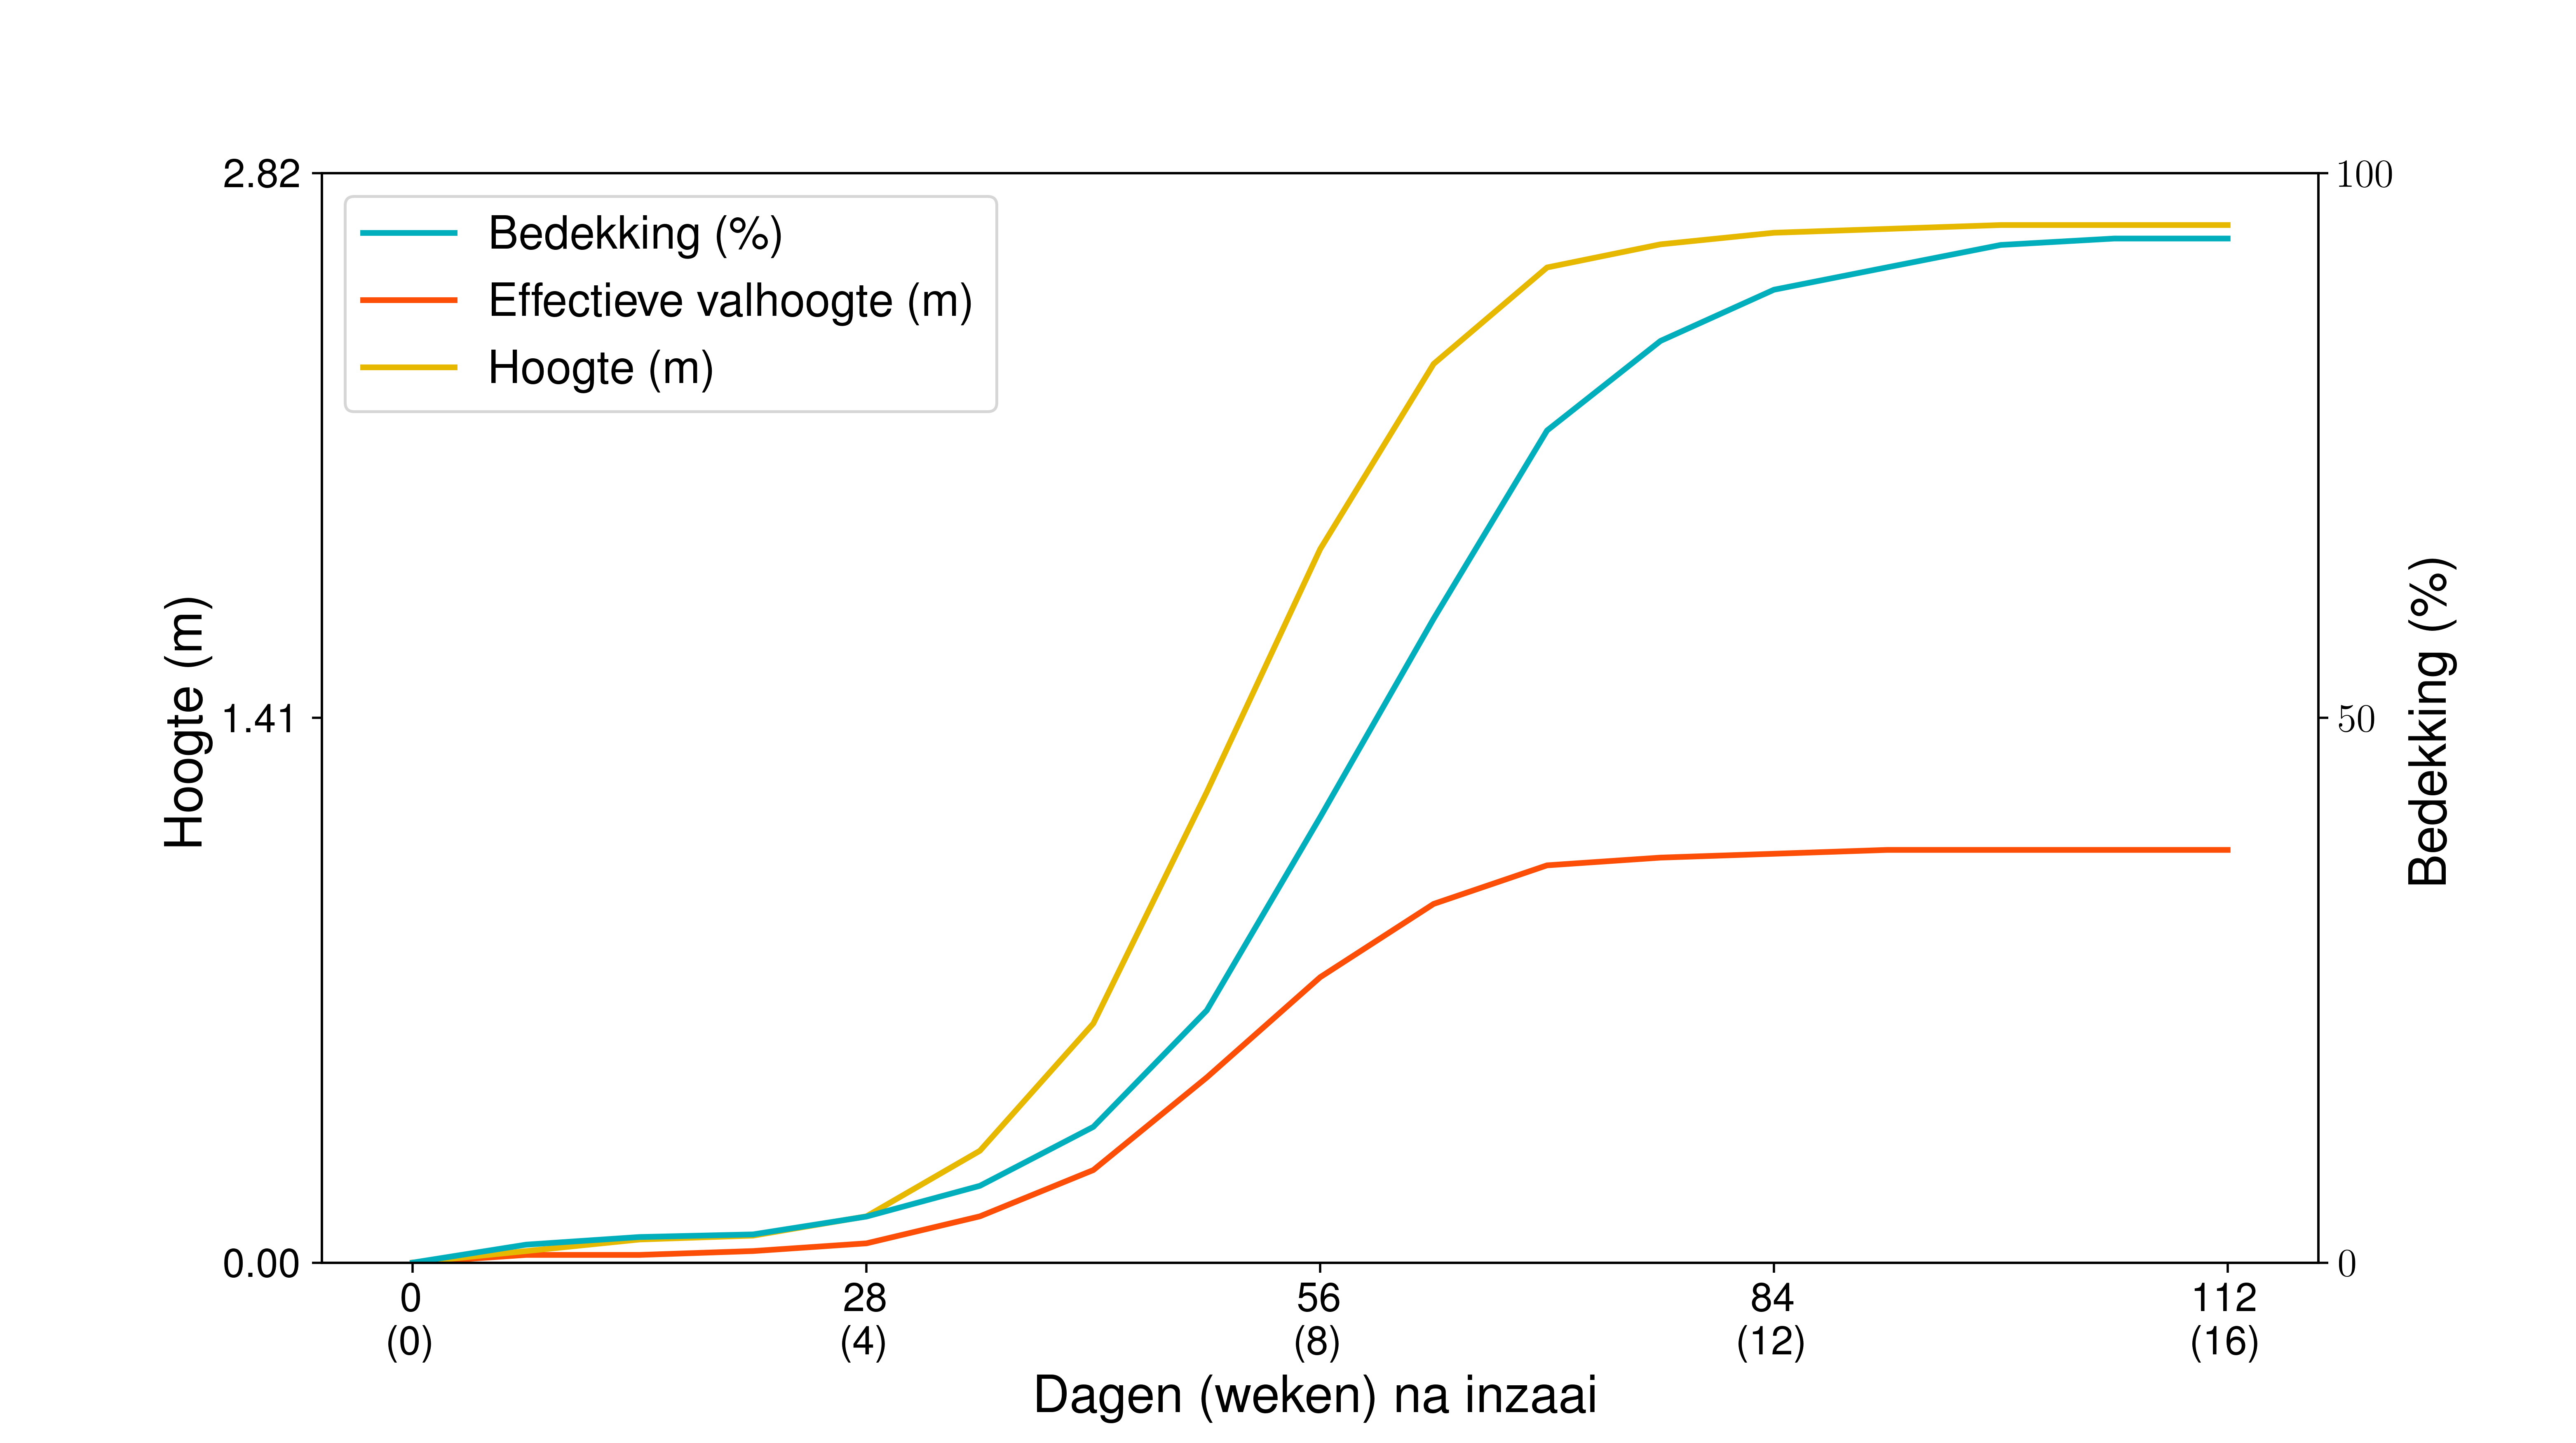
\includegraphics[width=12.5cm]{temp/2001.png} \end{figure} \end{center} 
  \textbf{Referenties:} ILVO2019 \vspace{0.10cm} \\ 
  \textbf{Opmerkingen?} verloop gewasgroeicurves geinterpoleerd met verloop gewasgroeicurve opgelijst in Verbist et al. (2004) en data Verstraeten et al. (2001) (zie code GV) \vspace{0.10cm} \\ 
 \newpage 
 \section{Korrelmais (groep\_id 2)} 
 \textbf{Van toepassing op gewasnamen (en codes):} Korrelmais (202) 
 \begin{multicols}{3} \begin{itemize} \item[$\square$] Meerjarig \item[$\square$] Groenbedekker \item[$\square$] Groente \end{itemize} \end{multicols} 
  \textbf{Zaaidatum (dd/mm)}: 01/05  \vspace{0.10cm} \\ 
  \textbf{Oogstdatum (dd/mm)}: 15/10  \vspace{0.10cm} \\ 
  \textbf{Oogstresten} \vspace{0.05cm} \\ 
  \tab Initi\"{e}le hoeveelheid (kg ha$^{-1}$): 9860.00 \vspace{0.05cm} \\ 
  \tab Afbraakcoefficient (-): 0.01 \vspace{0.05cm} \\ 
  \tab Bodembedekking (m$^2$ kg$^{-1}$): 3.04 \vspace{0.05cm} \\ 
  \tab Initieel percentage bedekking (\%): 95 \vspace{0.05cm} \\ 
  \tab Halfwaarde tijd (dagen): 30 \vspace{0.05cm} \\ 
  \textbf{Initi\"{e}le bodemruwheid (mm)}: 10.20 \vspace{0.05cm} \\ 
  \textbf{Gewasgroeicurve subgroep\_id 2001:} 
 \begin{center} \begin{figure}[H] 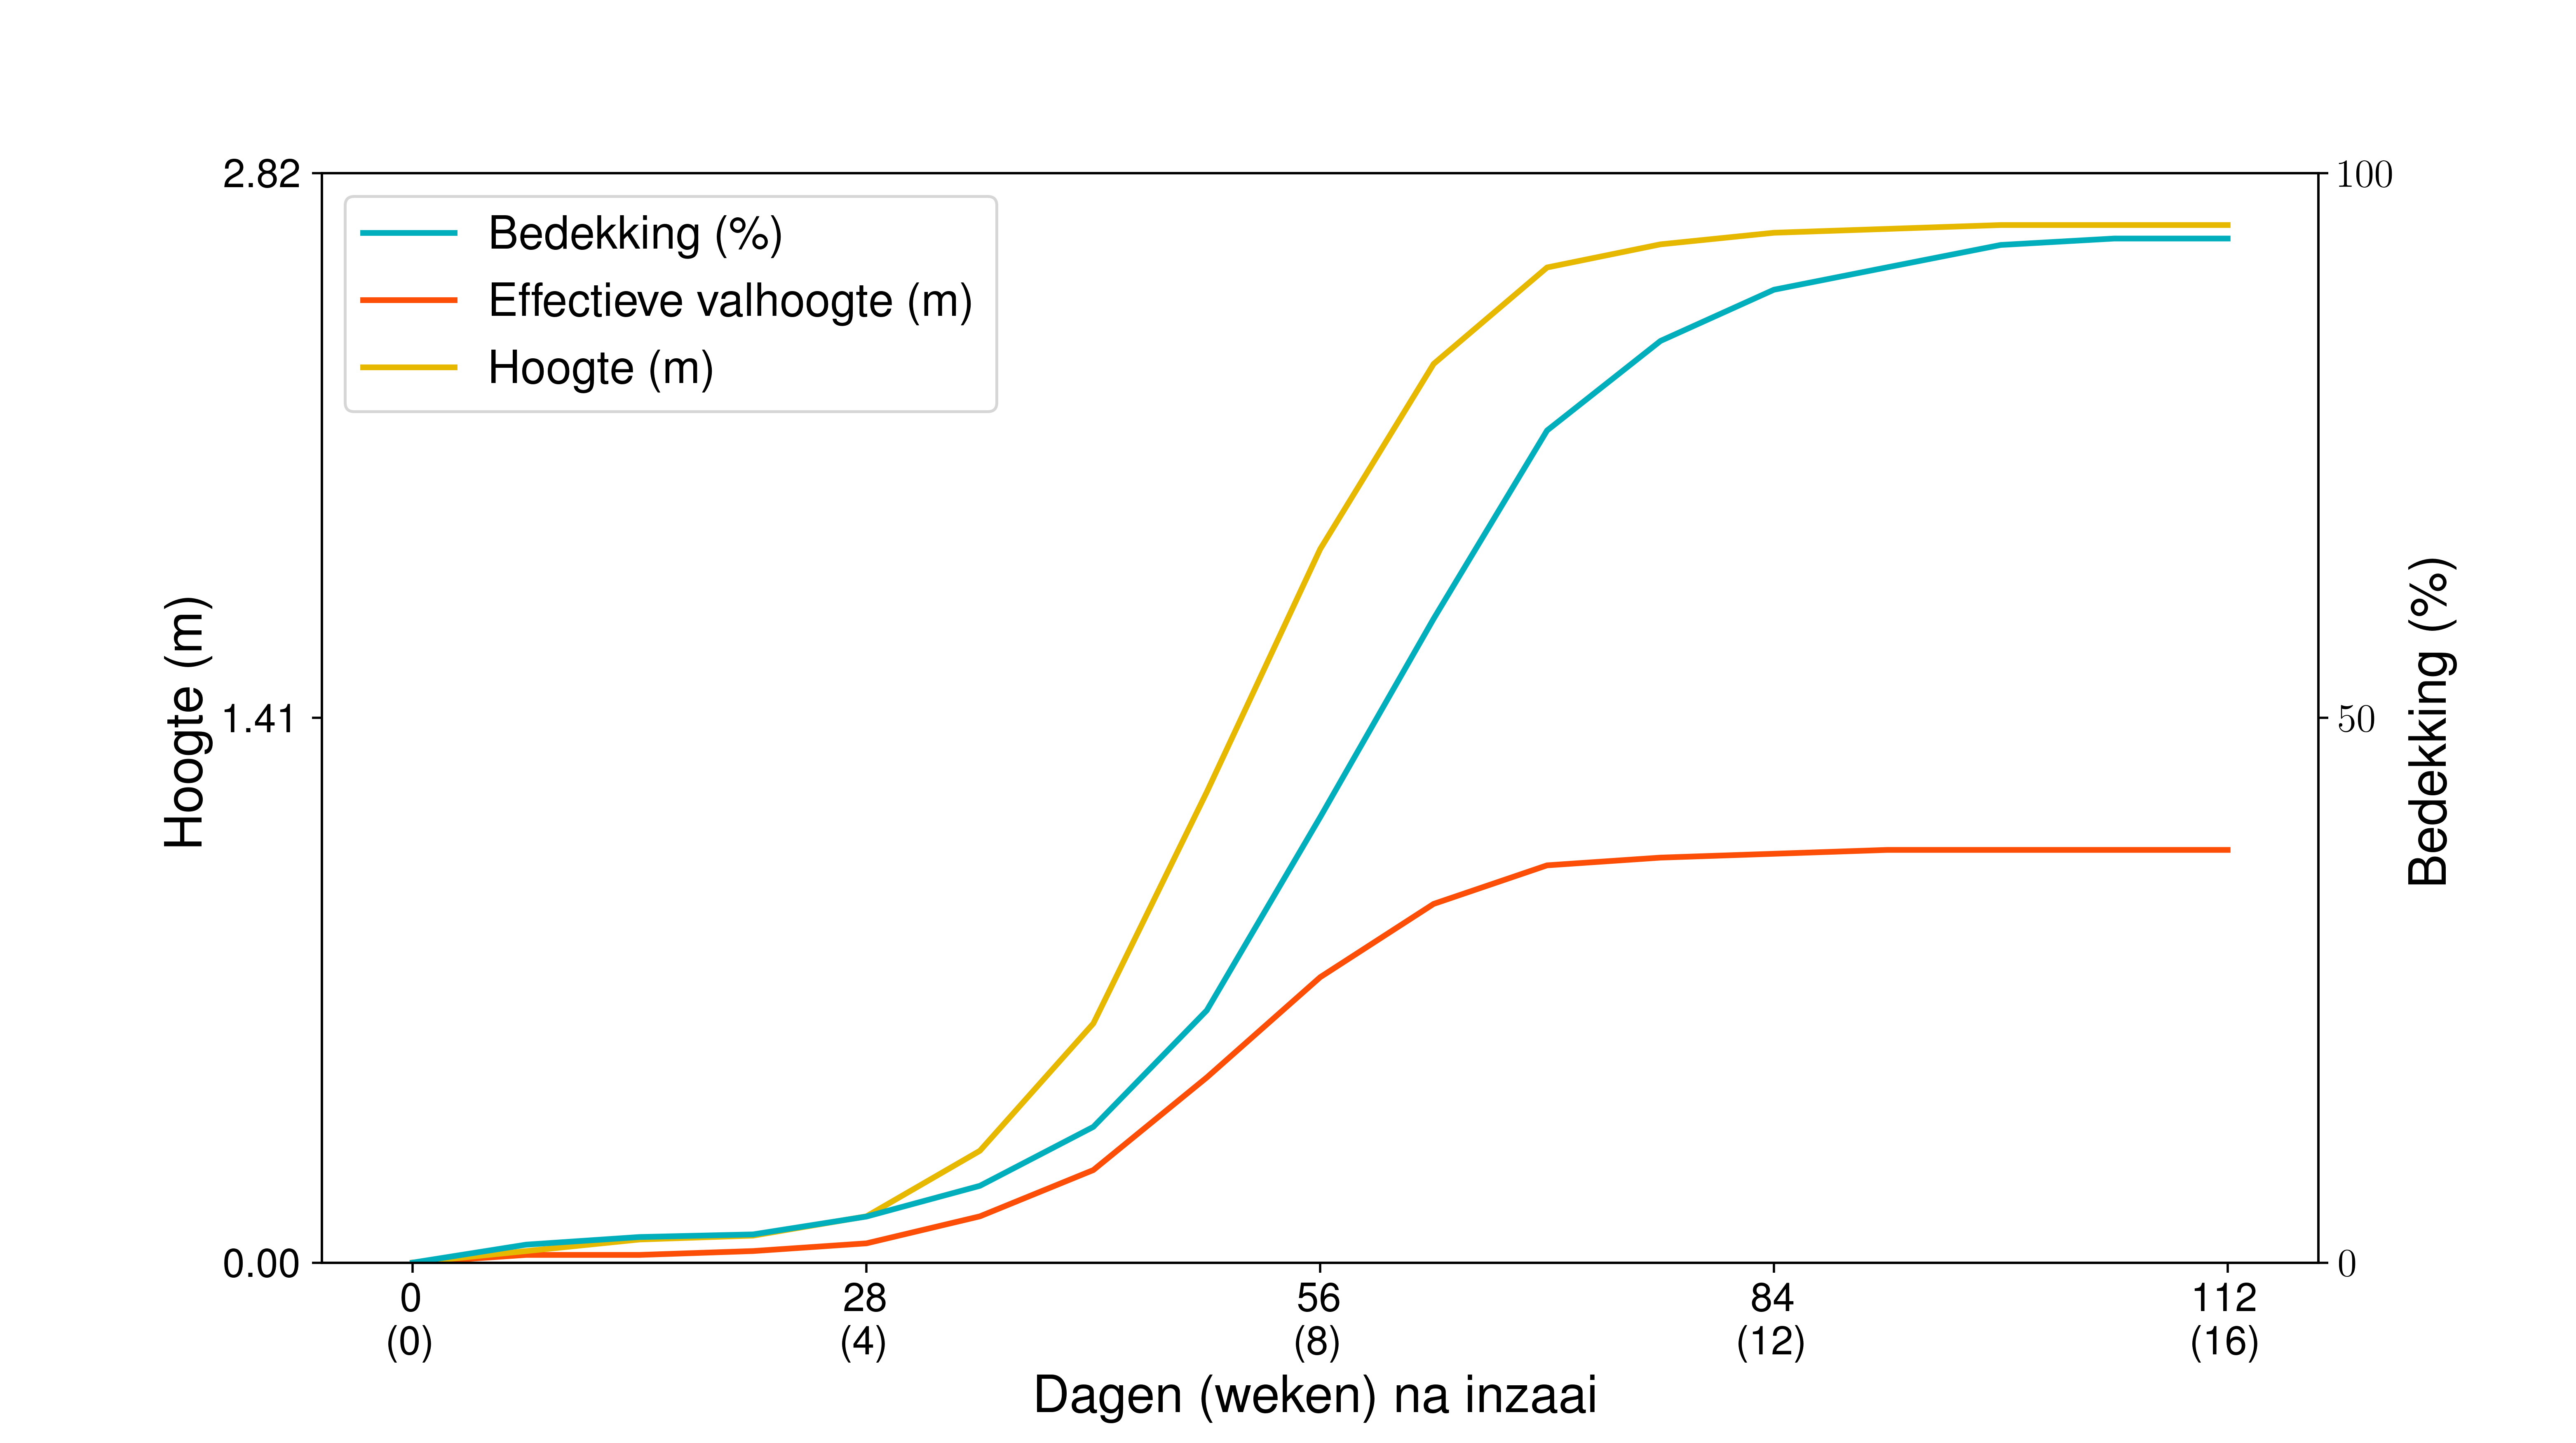
\includegraphics[width=12.5cm]{temp/2001.png} \end{figure} \end{center} 
  \textbf{Referenties:} ILVO2019 \vspace{0.10cm} \\ 
  \textbf{Opmerkingen?} verloop gewasgroeicurves geinterpoleerd met verloop gewasgroeicurve opgelijst in Verbist et al. (2004) en data Verstraeten et al. (2001) (zie code GV) \vspace{0.10cm} \\ 
 \newpage 
 \section{Aardappelen (niet-vroege) (groep\_id 3)} 
 \textbf{Van toepassing op gewasnamen (en codes):} Aardappelen (niet-vroege) (901) 
 \begin{multicols}{3} \begin{itemize} \item[$\square$] Meerjarig \item[$\square$] Groenbedekker \item[$\square$] Groente \end{itemize} \end{multicols} 
  \textbf{Zaaidatum (dd/mm)}: 15/04  \vspace{0.10cm} \\ 
  \textbf{Oogstdatum (dd/mm)}: 01/10  \vspace{0.10cm} \\ 
  \textbf{Oogstresten} \vspace{0.05cm} \\ 
  \tab Initi\"{e}le hoeveelheid (kg ha$^{-1}$): 2000.00 \vspace{0.05cm} \\ 
  \tab Afbraakcoefficient (-): 0.03 \vspace{0.05cm} \\ 
  \tab Bodembedekking (m$^2$ kg$^{-1}$): 0.30 \vspace{0.05cm} \\ 
  \tab Initieel percentage bedekking (\%): 6 \vspace{0.05cm} \\ 
  \tab Halfwaarde tijd (dagen): 10 \vspace{0.05cm} \\ 
  \textbf{Initi\"{e}le bodemruwheid (mm)}: 10.20 \vspace{0.05cm} \\ 
  \textbf{Gewasgroeicurve subgroep\_id 1003:} 
 \begin{center} \begin{figure}[H] 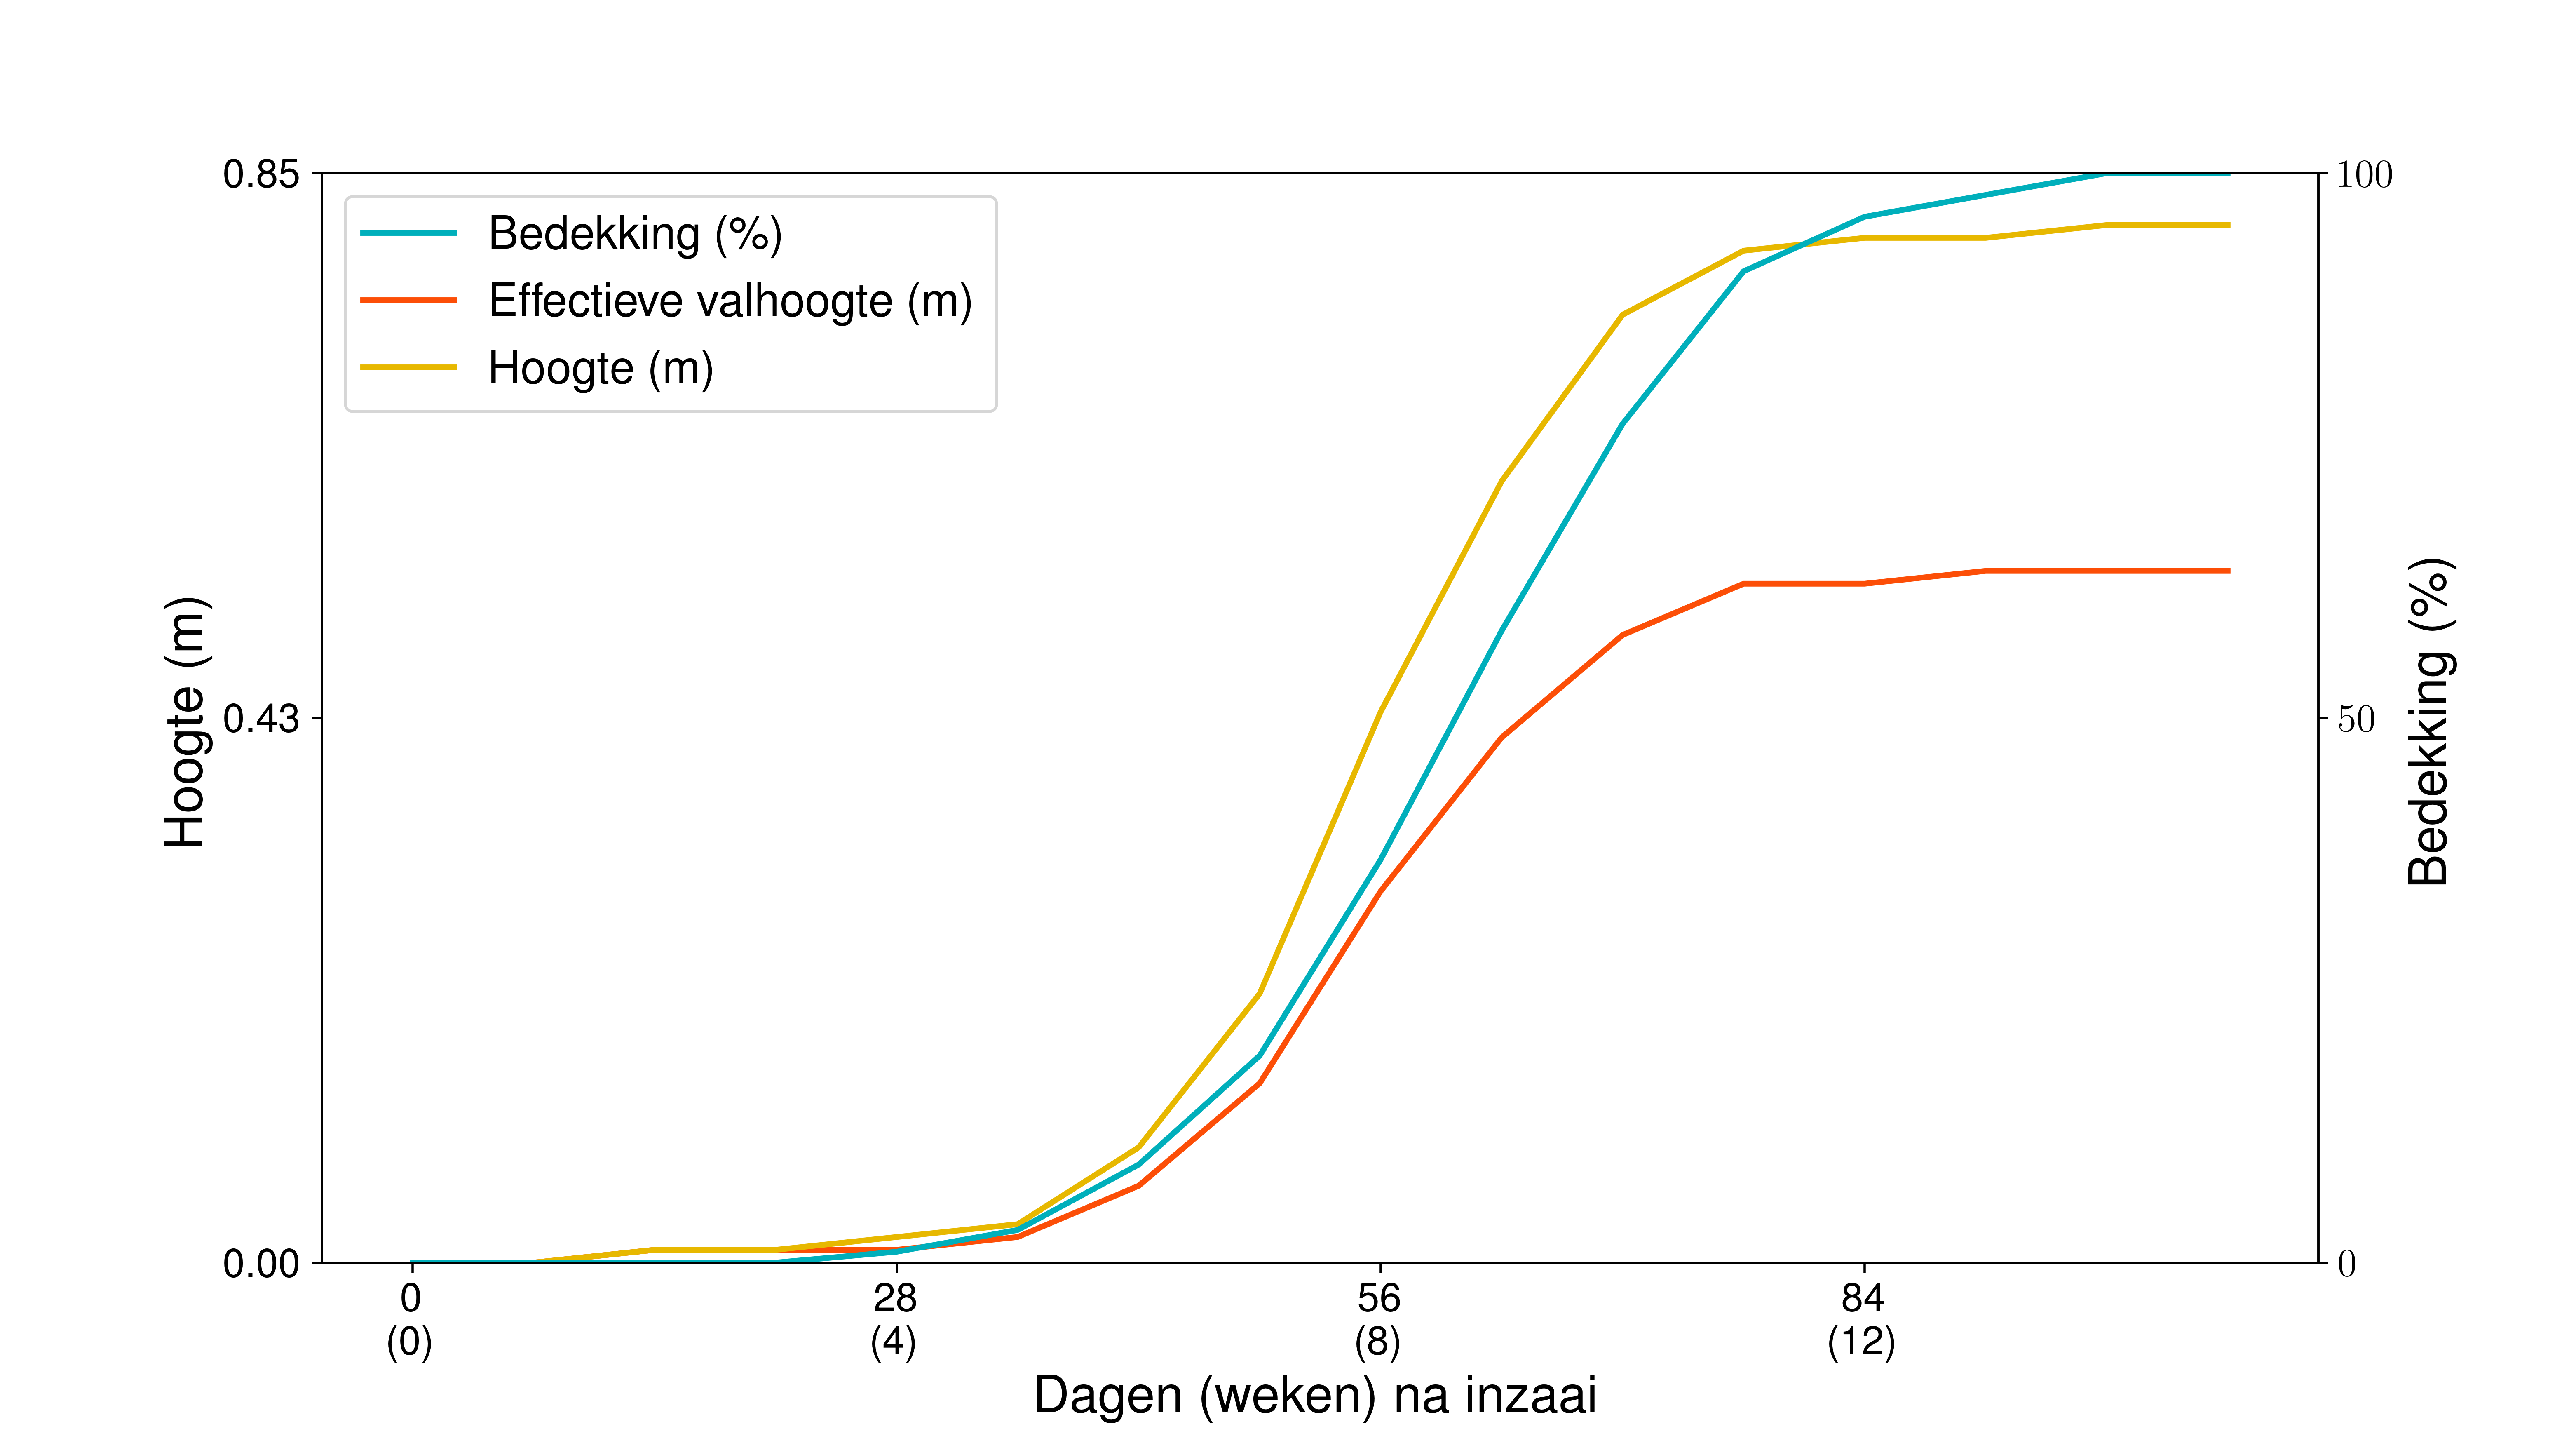
\includegraphics[width=12.5cm]{temp/1003.png} \end{figure} \end{center} 
  \textbf{Referenties:} ILVO2019 \vspace{0.10cm} \\ 
  \textbf{Opmerkingen?} geen \vspace{0.10cm} \\ 
 \newpage 
 \section{Aardappelen (pootgoed) (groep\_id 4)} 
 \textbf{Van toepassing op gewasnamen (en codes):} Aardappelen (pootgoed) (902) 
 \begin{multicols}{3} \begin{itemize} \item[$\square$] Meerjarig \item[$\square$] Groenbedekker \item[$\square$] Groente \end{itemize} \end{multicols} 
  \textbf{Zaaidatum (dd/mm)}: 01/04  \vspace{0.10cm} \\ 
  \textbf{Oogstdatum (dd/mm)}: 15/08  \vspace{0.10cm} \\ 
  \textbf{Oogstresten} \vspace{0.05cm} \\ 
  \tab Initi\"{e}le hoeveelheid (kg ha$^{-1}$): 2000.00 \vspace{0.05cm} \\ 
  \tab Afbraakcoefficient (-): 0.03 \vspace{0.05cm} \\ 
  \tab Bodembedekking (m$^2$ kg$^{-1}$): 0.30 \vspace{0.05cm} \\ 
  \tab Initieel percentage bedekking (\%): 6 \vspace{0.05cm} \\ 
  \tab Halfwaarde tijd (dagen): 10 \vspace{0.05cm} \\ 
  \textbf{Initi\"{e}le bodemruwheid (mm)}: 10.20 \vspace{0.05cm} \\ 
  \textbf{Gewasgroeicurve subgroep\_id 1003:} 
 \begin{center} \begin{figure}[H] 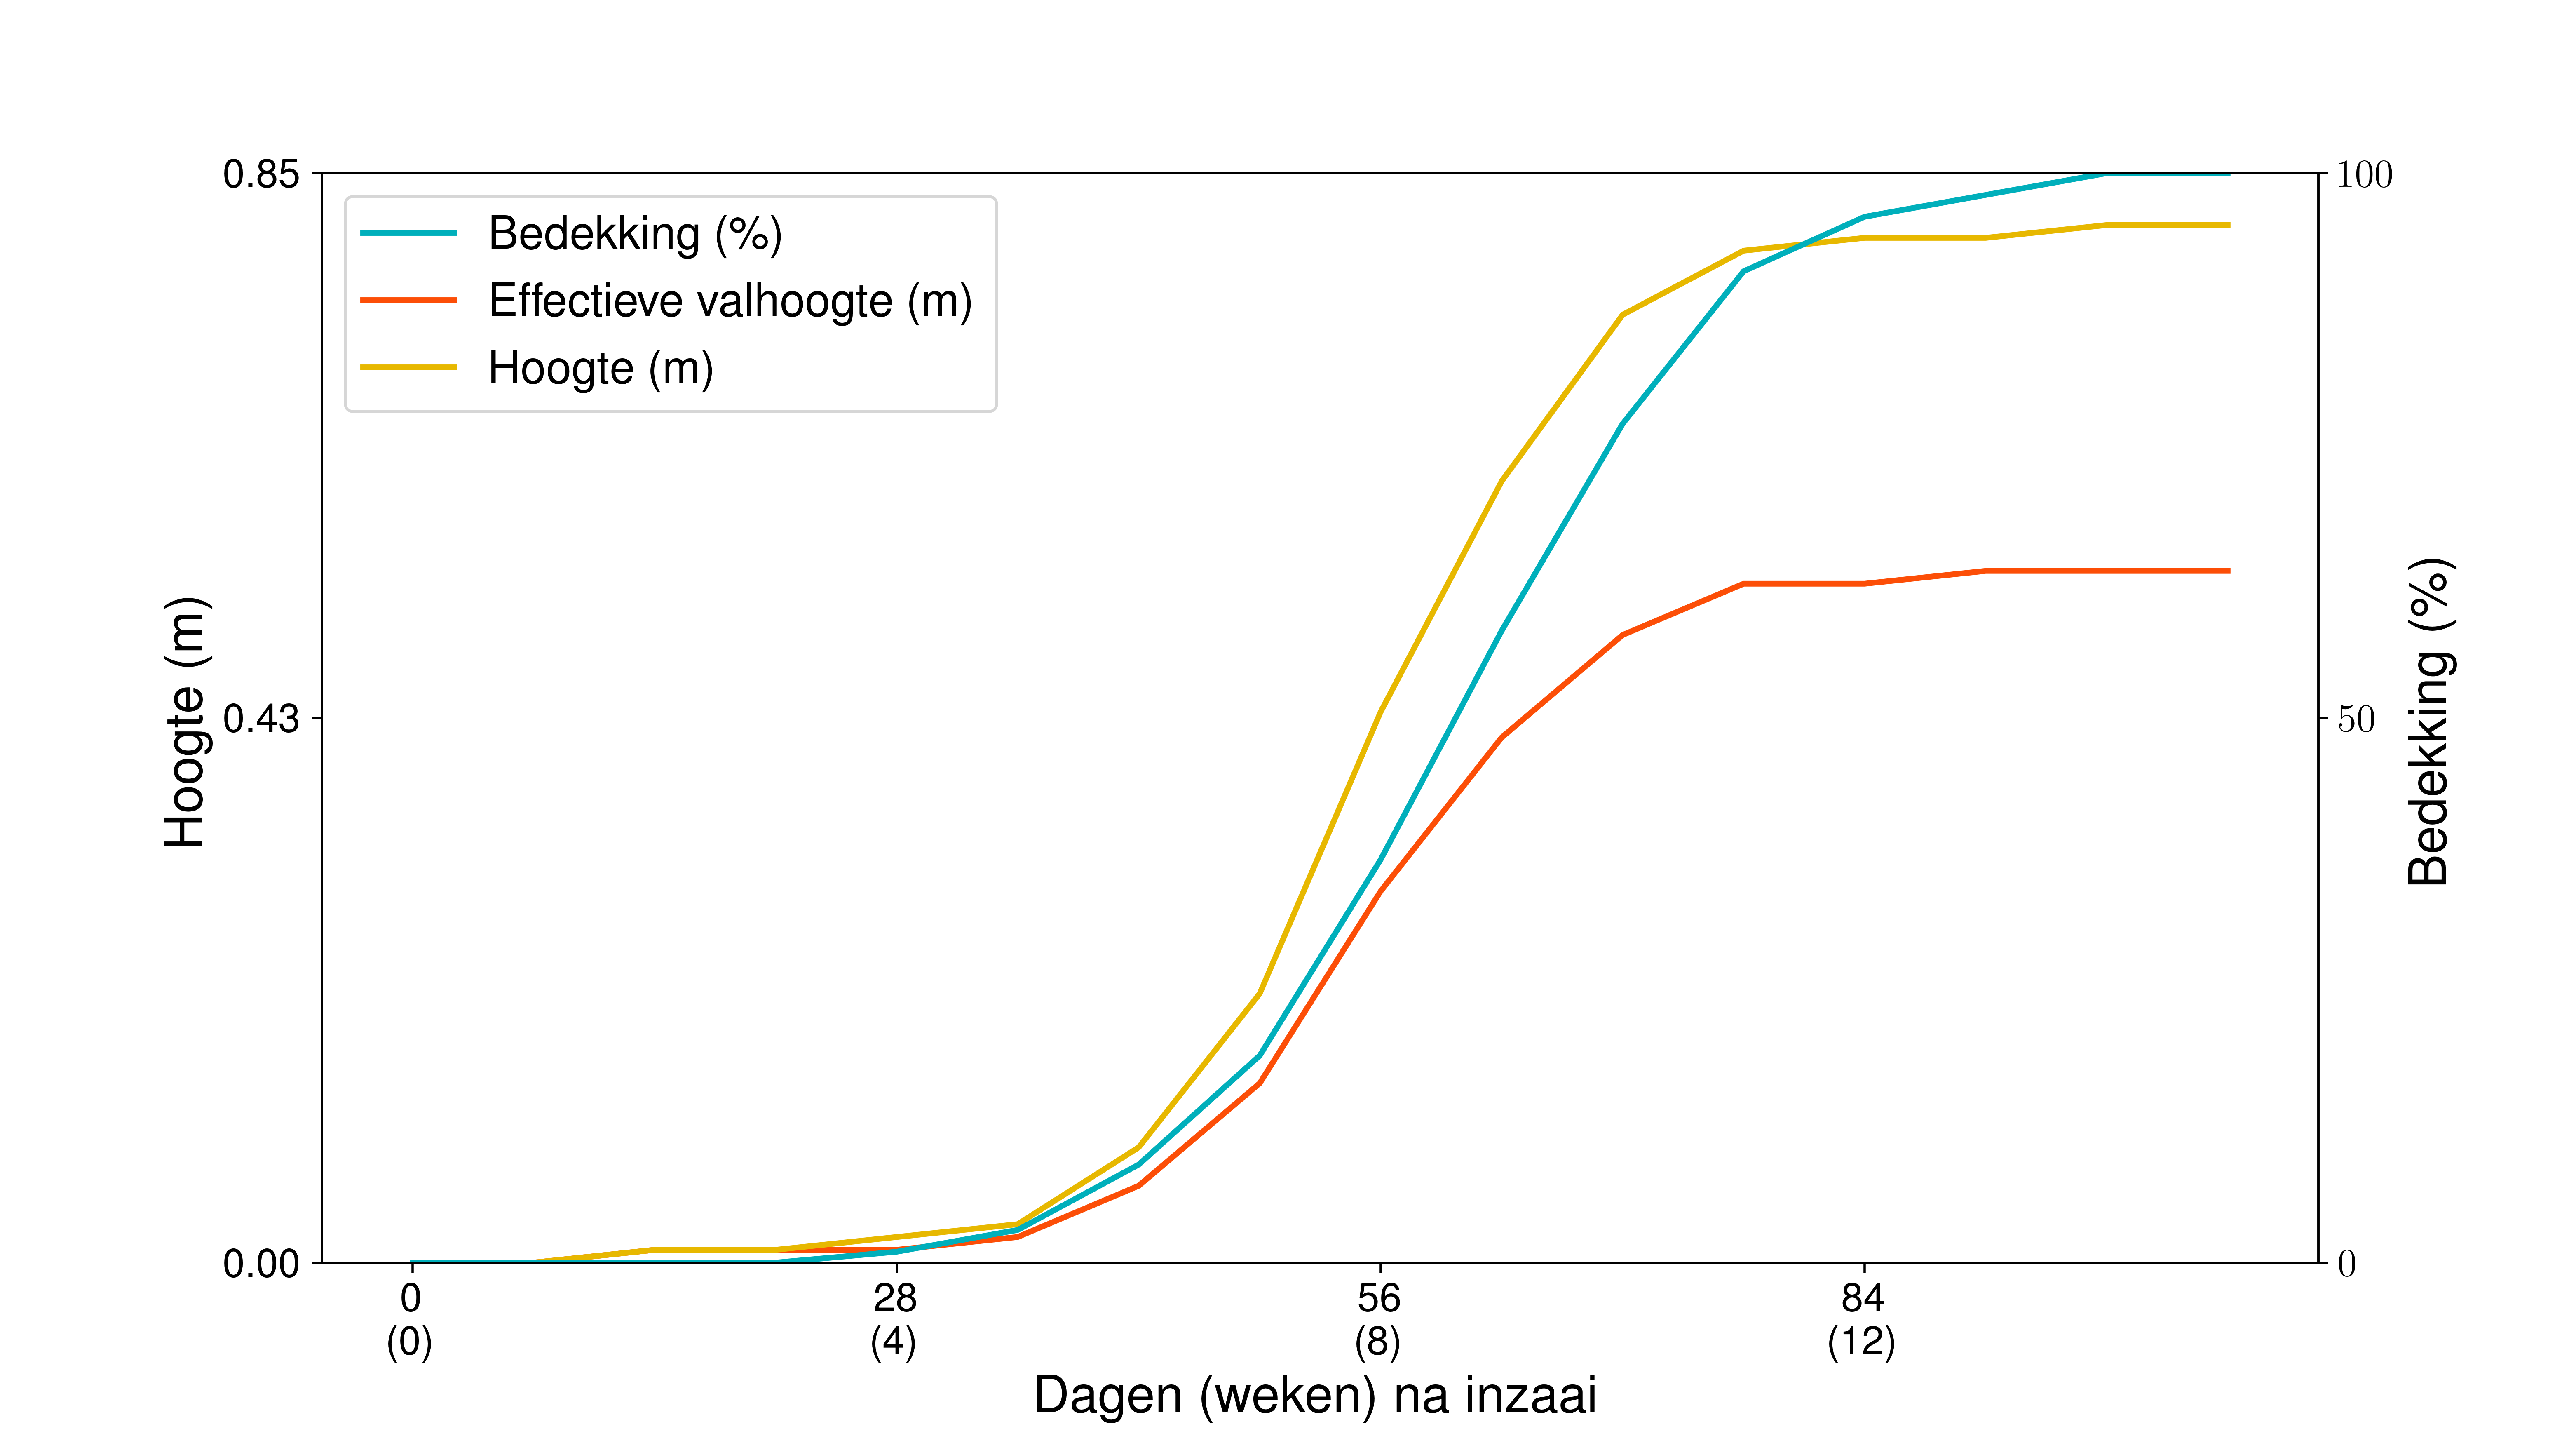
\includegraphics[width=12.5cm]{temp/1003.png} \end{figure} \end{center} 
  \textbf{Referenties:} ILVO2019 \vspace{0.10cm} \\ 
  \textbf{Opmerkingen?} geen \vspace{0.10cm} \\ 
 \newpage 
 \section{Aardappelen (vroege) (groep\_id 5)} 
 \textbf{Van toepassing op gewasnamen (en codes):} Aardappelen (vroege, rooi na 1906) (904) 
 \begin{multicols}{3} \begin{itemize} \item[$\square$] Meerjarig \item[$\square$] Groenbedekker \item[$\square$] Groente \end{itemize} \end{multicols} 
  \textbf{Zaaidatum (dd/mm)}: 01/04  \vspace{0.10cm} \\ 
  \textbf{Oogstdatum (dd/mm)}: 01/08  \vspace{0.10cm} \\ 
  \textbf{Oogstresten} \vspace{0.05cm} \\ 
  \tab Initi\"{e}le hoeveelheid (kg ha$^{-1}$): 2000.00 \vspace{0.05cm} \\ 
  \tab Afbraakcoefficient (-): 0.03 \vspace{0.05cm} \\ 
  \tab Bodembedekking (m$^2$ kg$^{-1}$): 0.30 \vspace{0.05cm} \\ 
  \tab Initieel percentage bedekking (\%): 6 \vspace{0.05cm} \\ 
  \tab Halfwaarde tijd (dagen): 10 \vspace{0.05cm} \\ 
  \textbf{Initi\"{e}le bodemruwheid (mm)}: 10.20 \vspace{0.05cm} \\ 
  \textbf{Gewasgroeicurve subgroep\_id 1003:} 
 \begin{center} \begin{figure}[H] 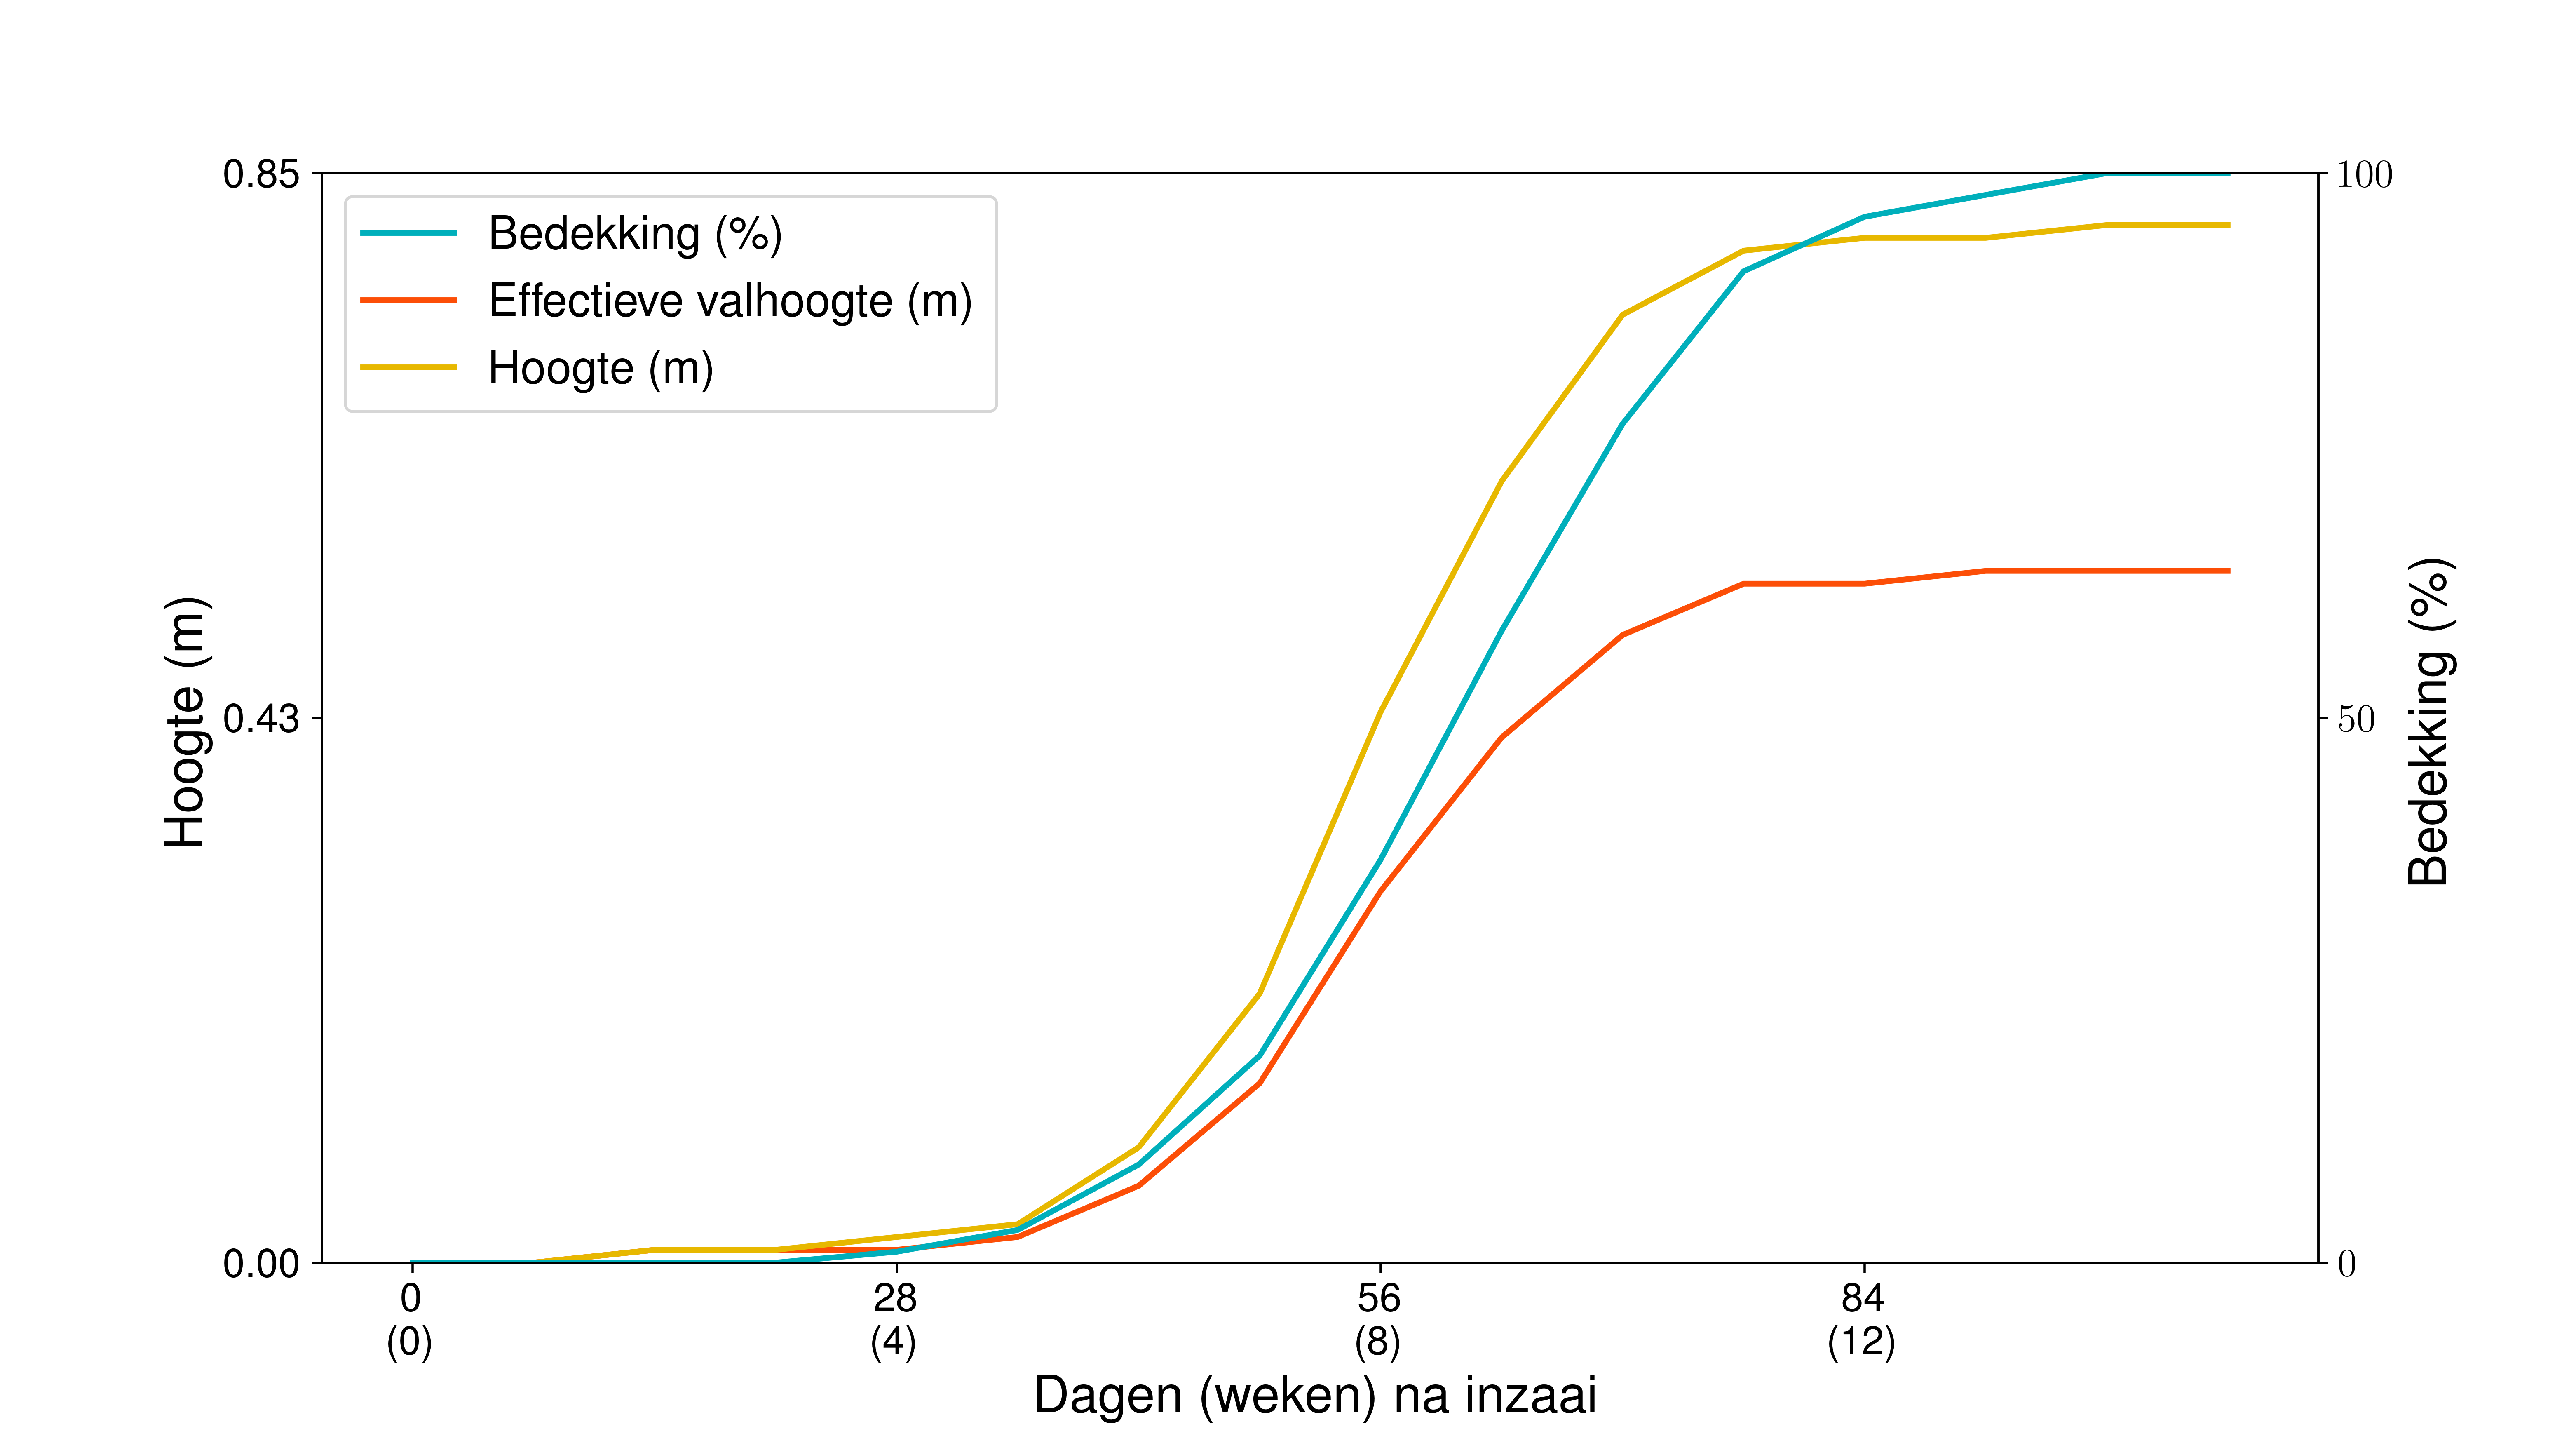
\includegraphics[width=12.5cm]{temp/1003.png} \end{figure} \end{center} 
  \textbf{Referenties:} ILVO2019 \vspace{0.10cm} \\ 
  \textbf{Opmerkingen?} geen \vspace{0.10cm} \\ 
 \newpage 
 \section{Voederbieten (groep\_id 6)} 
 \textbf{Van toepassing op gewasnamen (en codes):} Voederbieten (71) 
 \begin{multicols}{3} \begin{itemize} \item[$\square$] Meerjarig \item[$\square$] Groenbedekker \item[$\square$] Groente \end{itemize} \end{multicols} 
  \textbf{Zaaidatum (dd/mm)}: 01/04  \vspace{0.10cm} \\ 
  \textbf{Oogstdatum (dd/mm)}: 01/11  \vspace{0.10cm} \\ 
  \textbf{Oogstresten} \vspace{0.05cm} \\ 
  \tab Initi\"{e}le hoeveelheid (kg ha$^{-1}$): 2600.00 \vspace{0.05cm} \\ 
  \tab Afbraakcoefficient (-): 0.02 \vspace{0.05cm} \\ 
  \tab Bodembedekking (m$^2$ kg$^{-1}$): 2.30 \vspace{0.05cm} \\ 
  \tab Initieel percentage bedekking (\%): 45 \vspace{0.05cm} \\ 
  \tab Halfwaarde tijd (dagen): 15 \vspace{0.05cm} \\ 
  \textbf{Initi\"{e}le bodemruwheid (mm)}: 7.60 \vspace{0.05cm} \\ 
  \textbf{Gewasgroeicurve subgroep\_id 2006:} 
 \begin{center} \begin{figure}[H] 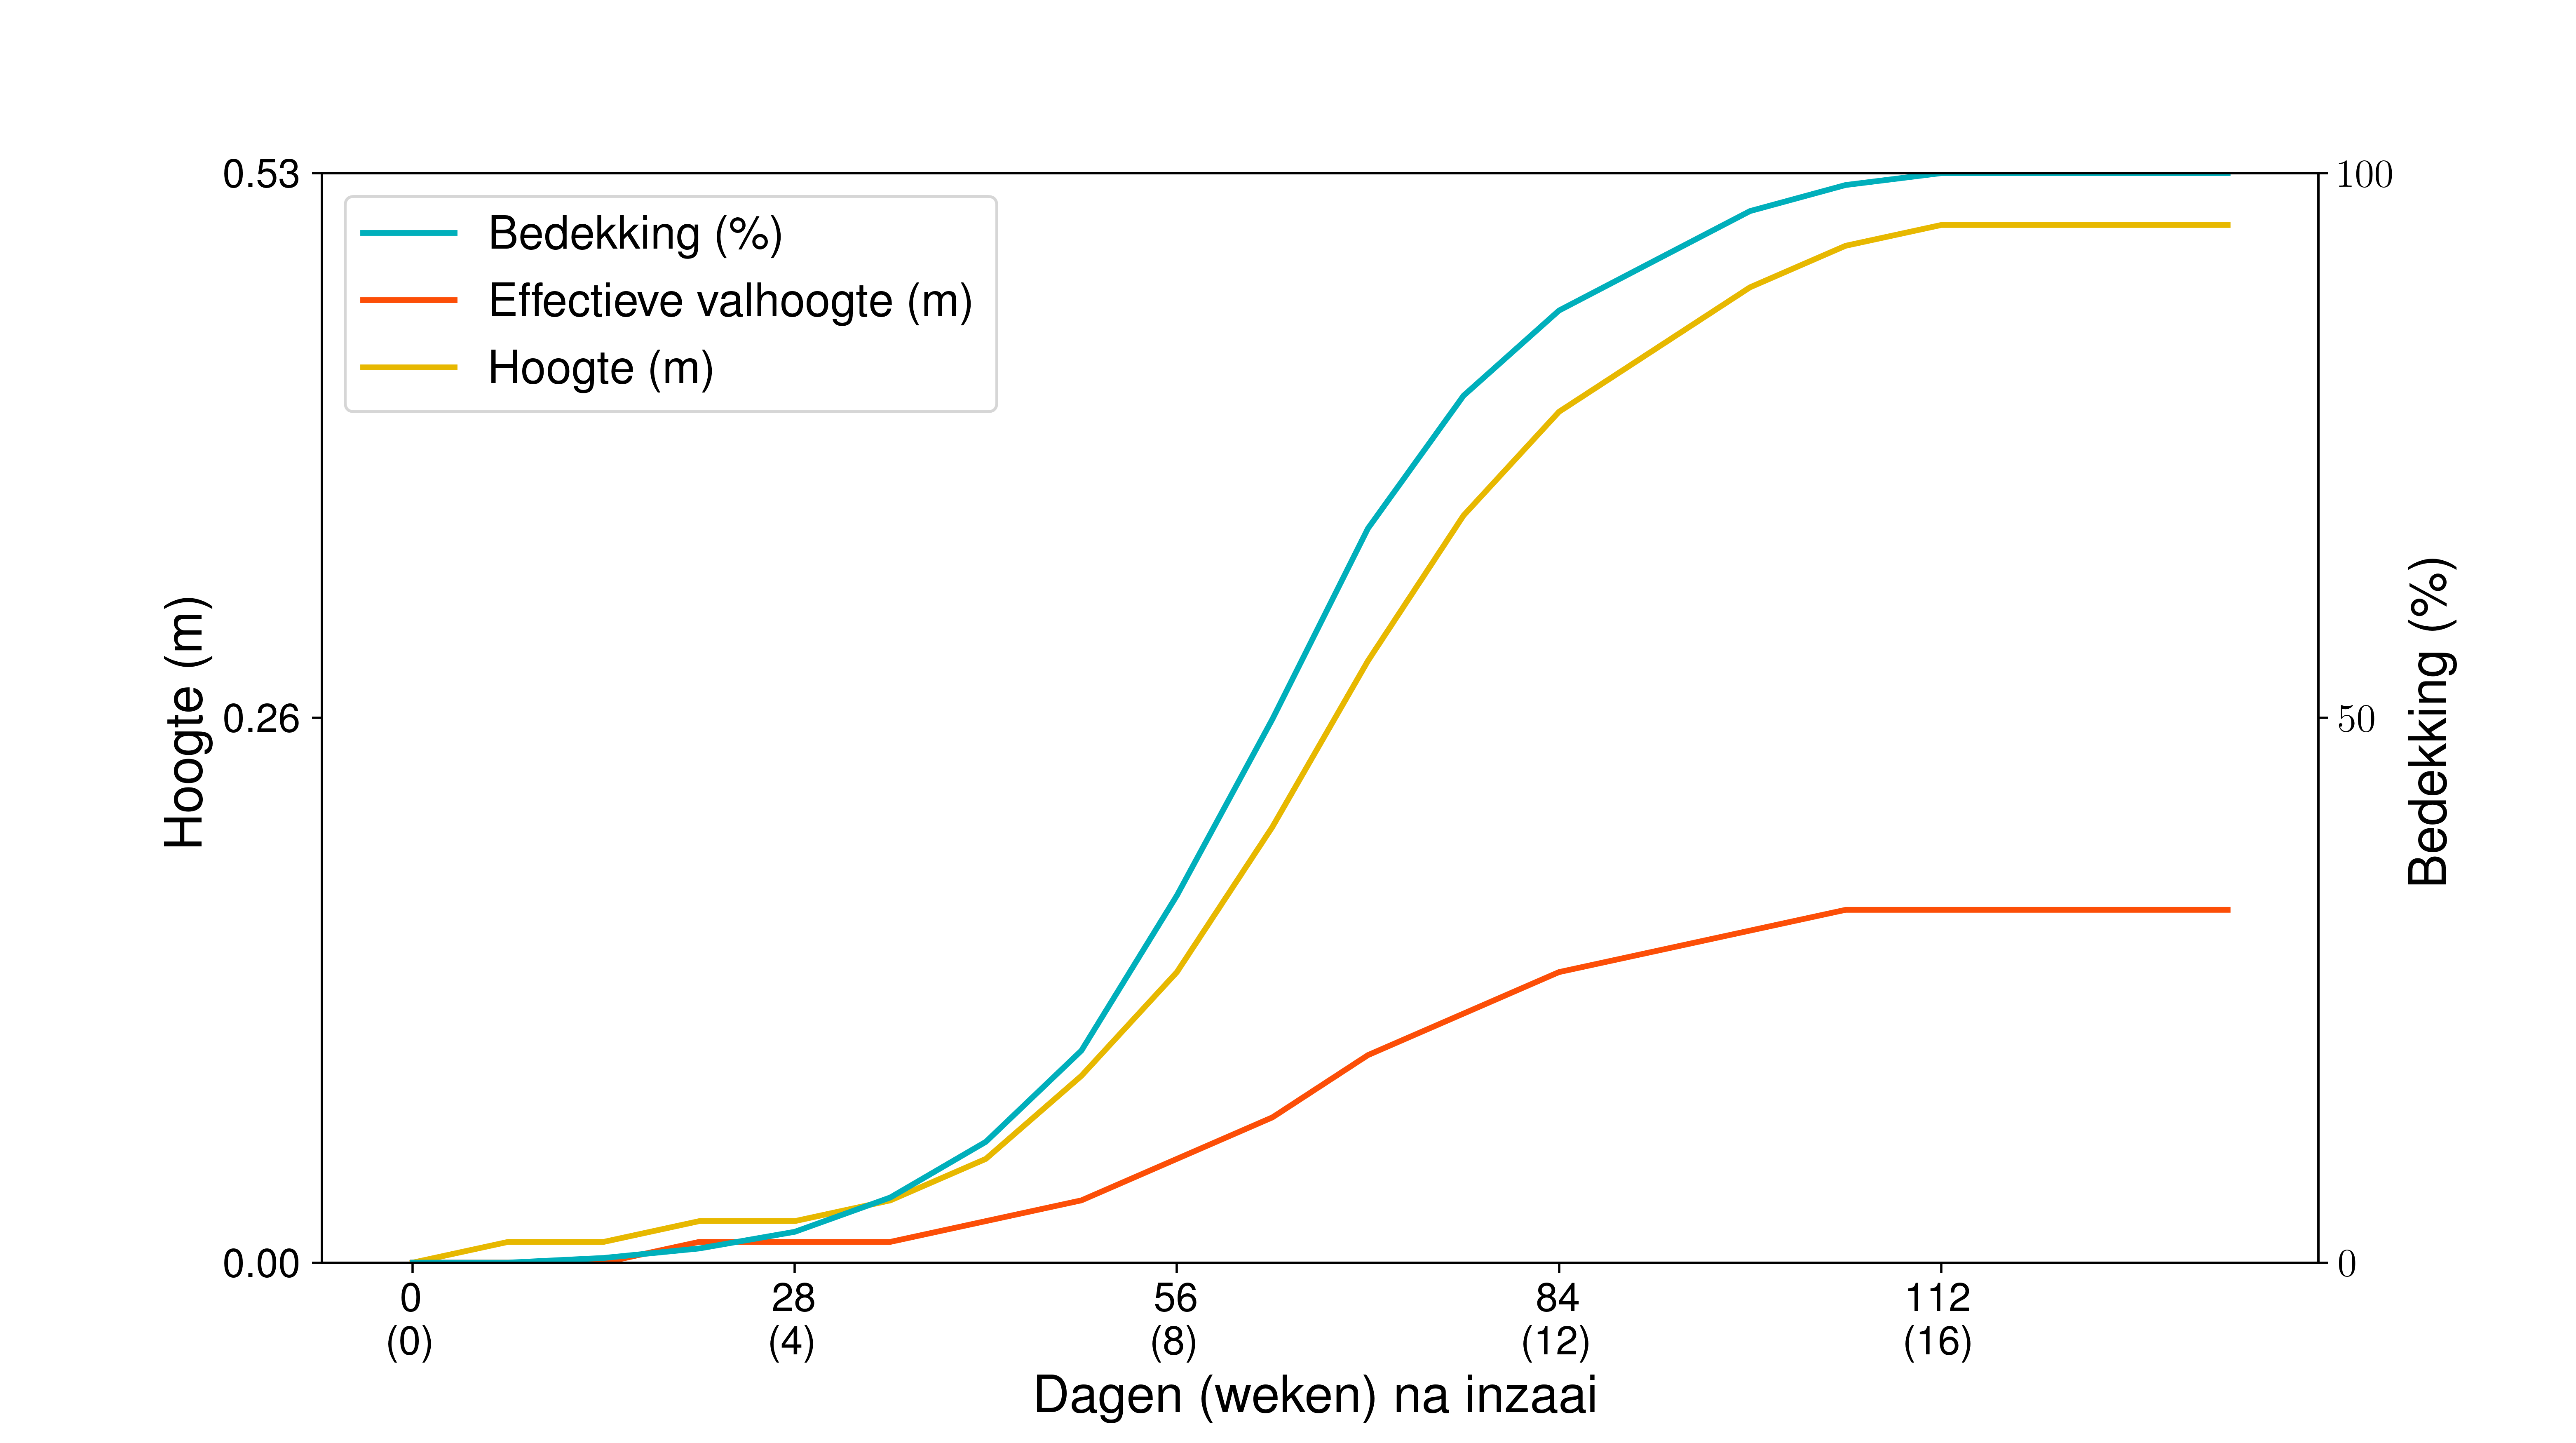
\includegraphics[width=12.5cm]{temp/2006.png} \end{figure} \end{center} 
  \textbf{Referenties:} ILVO2019 \vspace{0.10cm} \\ 
  \textbf{Opmerkingen?} verloop gewasgroeicurves geinterpoleerd met verloop gewasgroeicurve opgelijst in Verbist et al. (2004) en data Verstraeten et al. (2001) (zie code GV) \vspace{0.10cm} \\ 
 \newpage 
 \section{Suikerbieten (groep\_id 7)} 
 \textbf{Van toepassing op gewasnamen (en codes):} Suikerbieten (91) 
 \begin{multicols}{3} \begin{itemize} \item[$\square$] Meerjarig \item[$\square$] Groenbedekker \item[$\square$] Groente \end{itemize} \end{multicols} 
  \textbf{Zaaidatum (dd/mm)}: 01/04  \vspace{0.10cm} \\ 
  \textbf{Oogstdatum (dd/mm)}: 01/11  \vspace{0.10cm} \\ 
  \textbf{Oogstresten} \vspace{0.05cm} \\ 
  \tab Initi\"{e}le hoeveelheid (kg ha$^{-1}$): 5270.00 \vspace{0.05cm} \\ 
  \tab Afbraakcoefficient (-): 0.03 \vspace{0.05cm} \\ 
  \tab Bodembedekking (m$^2$ kg$^{-1}$): 1.78 \vspace{0.05cm} \\ 
  \tab Initieel percentage bedekking (\%): 61 \vspace{0.05cm} \\ 
  \tab Halfwaarde tijd (dagen): 10 \vspace{0.05cm} \\ 
  \textbf{Initi\"{e}le bodemruwheid (mm)}: 7.60 \vspace{0.05cm} \\ 
  \textbf{Gewasgroeicurve subgroep\_id 1007:} 
 \begin{center} \begin{figure}[H] 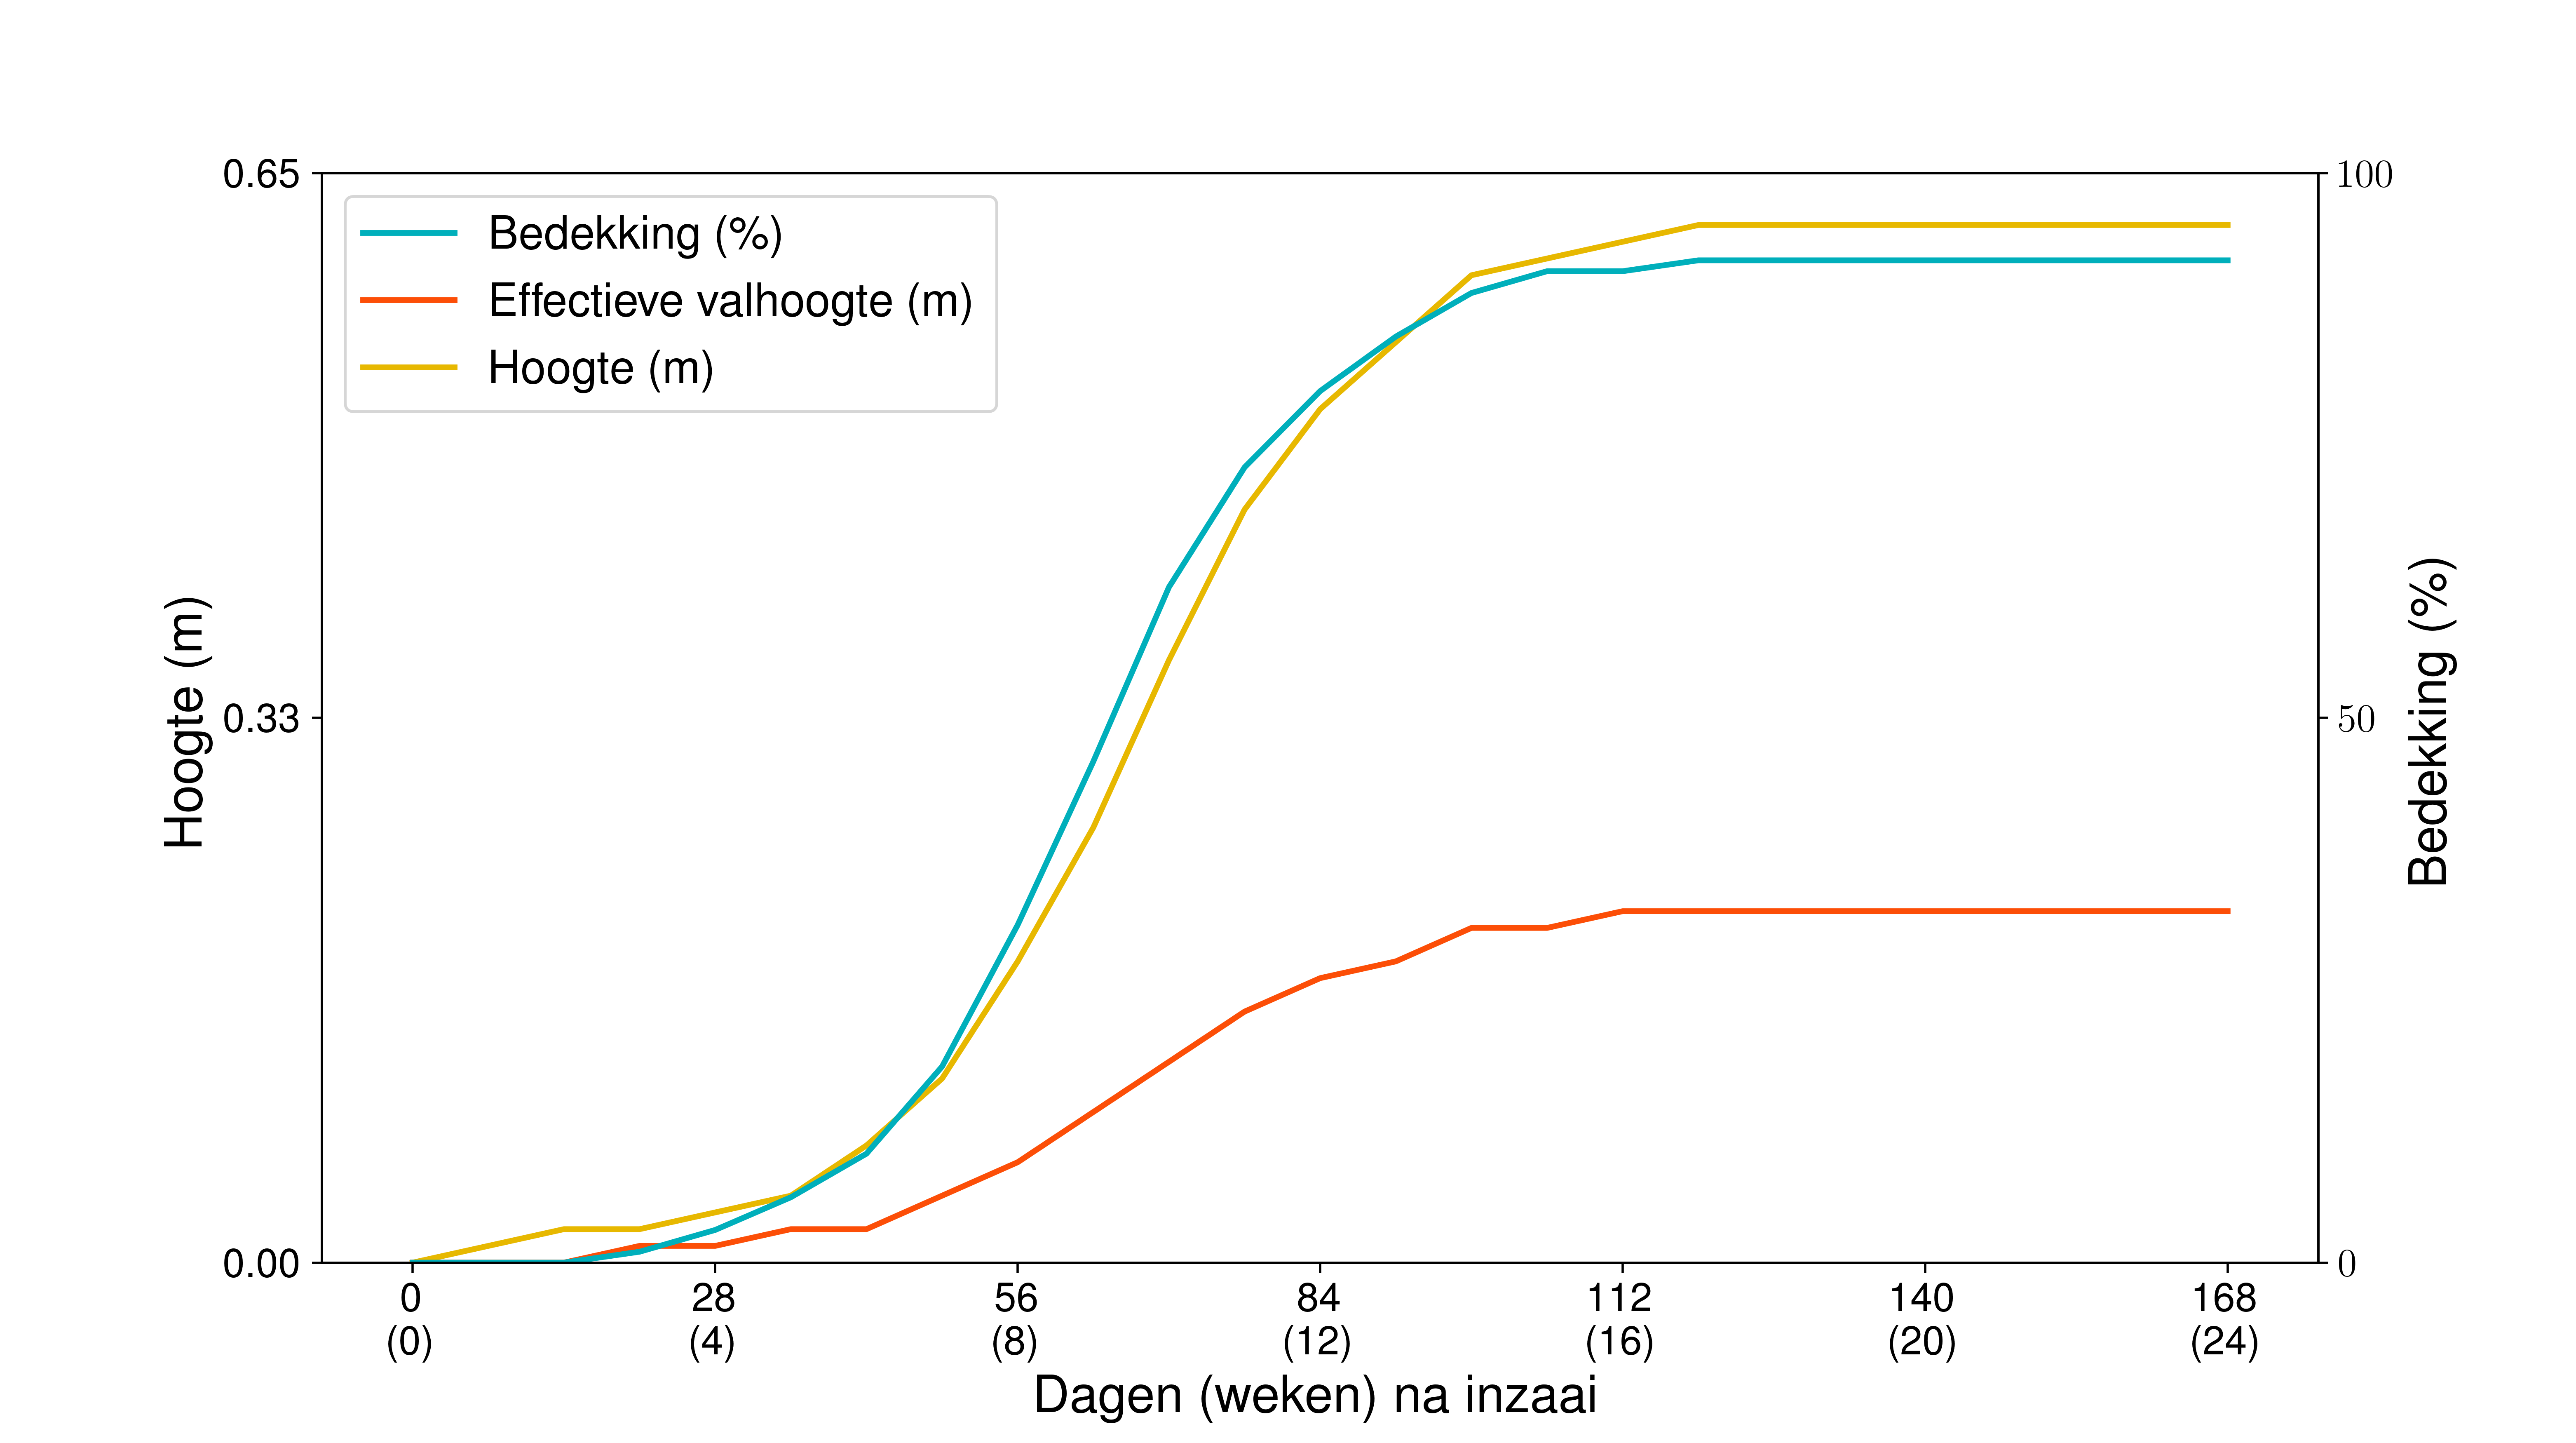
\includegraphics[width=12.5cm]{temp/1007.png} \end{figure} \end{center} 
  \textbf{Referenties:} ILVO2019 \vspace{0.10cm} \\ 
  \textbf{Opmerkingen?} verloop gewasgroeicurves geinterpoleerd met verloop gewasgroeicurve opgelijst in Verbist et al. (2004) en data Verstraeten et al. (2001) (zie code GV) \vspace{0.10cm} \\ 
 \newpage 
 \section{Wintertarwe, triticale en spelt (groep\_id 8)} 
 \textbf{Van toepassing op gewasnamen (en codes):} Wintertarwe (311) , Triticale (35) , Spelt (36) 
 \begin{multicols}{3} \begin{itemize} \item[$\square$] Meerjarig \item[$\square$] Groenbedekker \item[$\square$] Groente \end{itemize} \end{multicols} 
 \subsection{Hoofdteelt, voorteelt en nateelt (inzaaidatum=[1015,1030]) (subgroep\_id 1008)} 
  \textbf{Zaaidatum (dd/mm)}: 15/10  \vspace{0.10cm} \\ 
  \textbf{Oogstdatum (dd/mm)}: 01/08  \vspace{0.10cm} \\ 
  \textbf{Oogstresten} \vspace{0.05cm} \\ 
  \tab Initi\"{e}le hoeveelheid (kg ha$^{-1}$): 3600.00 \vspace{0.05cm} \\ 
  \tab Afbraakcoefficient (-): 0.01 \vspace{0.05cm} \\ 
  \tab Bodembedekking (m$^2$ kg$^{-1}$): 1.20 \vspace{0.05cm} \\ 
  \tab Initieel percentage bedekking (\%): 100 \vspace{0.05cm} \\ 
  \tab Halfwaarde tijd (dagen): 30 \vspace{0.05cm} \\ 
  \textbf{Initi\"{e}le bodemruwheid (mm)}: 10.20 \vspace{0.05cm} \\ 
  \textbf{Gewasgroeicurve subgroep\_id 1008:} 
 \begin{center} \begin{figure}[H] 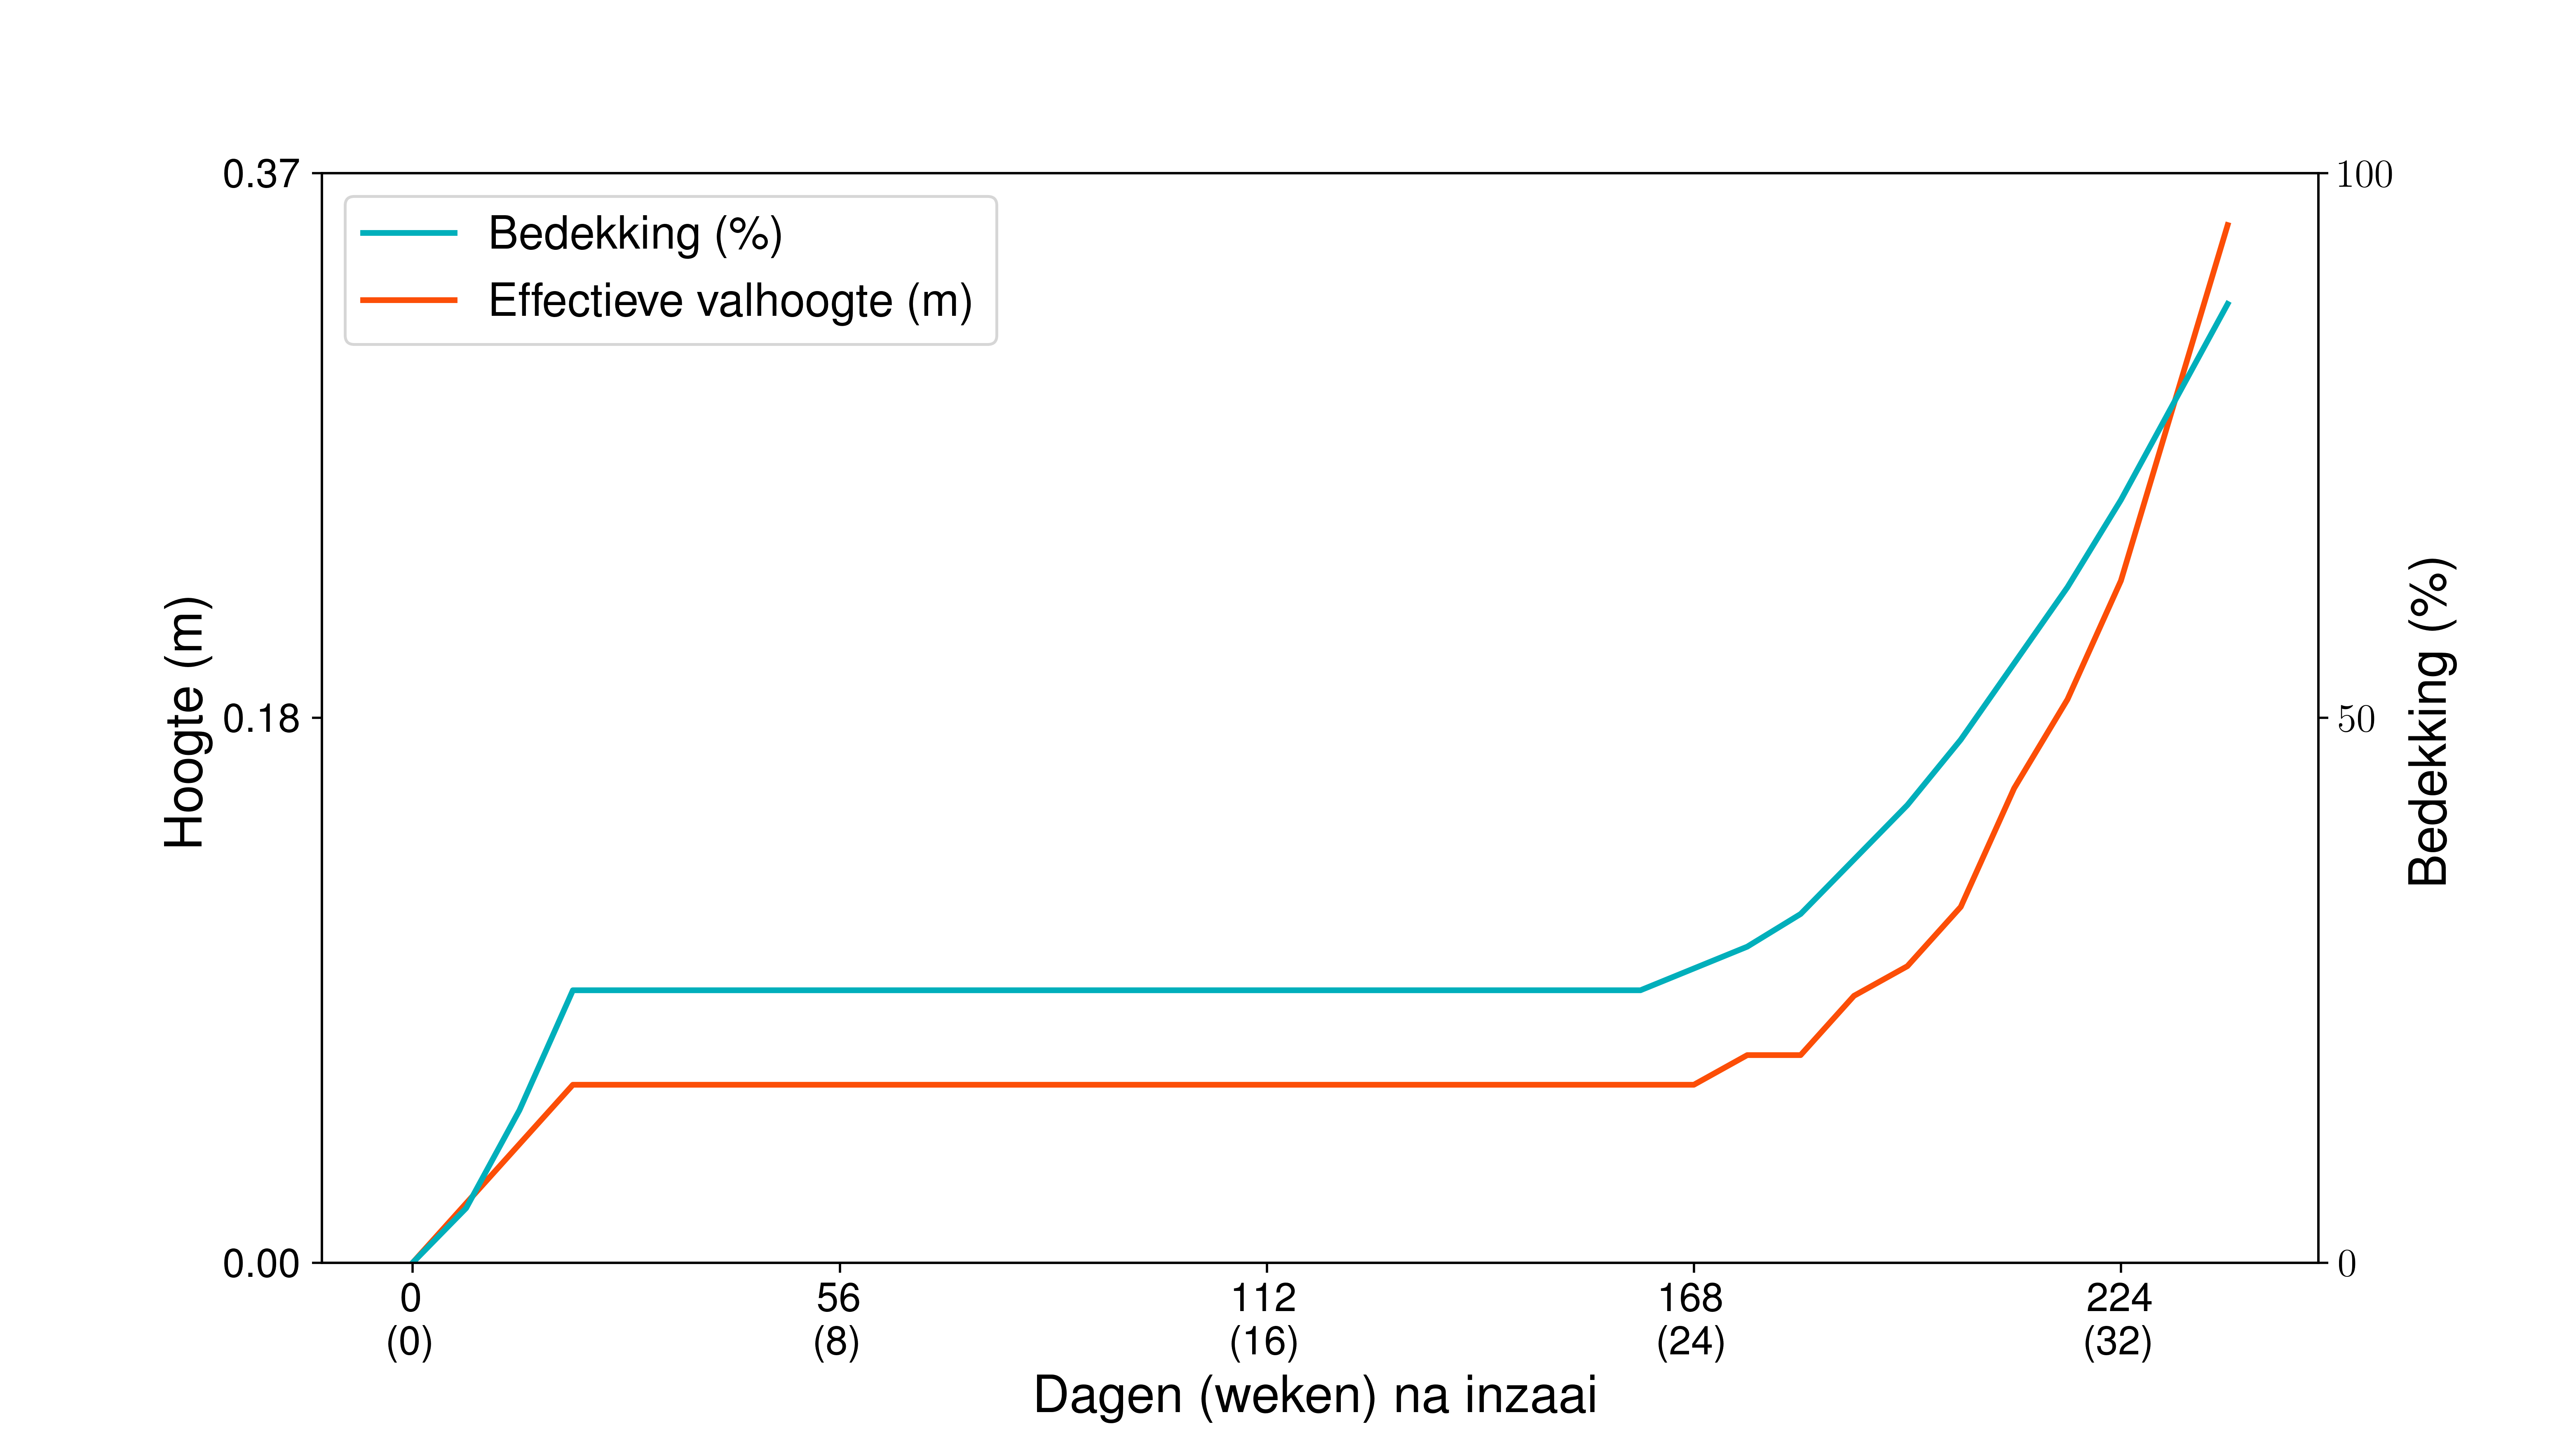
\includegraphics[width=12.5cm]{temp/1008.png} \end{figure} \end{center} 
  \textbf{Referenties:} Verbist2004;Gabriels2003;KMI2003;ILVO2019;Gobin2013 \vspace{0.10cm} \\ 
  \textbf{Opmerkingen?} geen \vspace{0.10cm} \\ 
 \newpage 
 \subsection{Hoofdteelt, voorteelt en nateelt (inzaaidatum=[1101,1231]) (subgroep\_id 2008)} 
  \textbf{Zaaidatum (dd/mm)}: 01/11  \vspace{0.10cm} \\ 
  \textbf{Oogstdatum (dd/mm)}: 01/08  \vspace{0.10cm} \\ 
  \textbf{Oogstresten} \vspace{0.05cm} \\ 
  \tab Initi\"{e}le hoeveelheid (kg ha$^{-1}$): 3600.00 \vspace{0.05cm} \\ 
  \tab Afbraakcoefficient (-): 0.01 \vspace{0.05cm} \\ 
  \tab Bodembedekking (m$^2$ kg$^{-1}$): 1.20 \vspace{0.05cm} \\ 
  \tab Initieel percentage bedekking (\%): 100 \vspace{0.05cm} \\ 
  \tab Halfwaarde tijd (dagen): 30 \vspace{0.05cm} \\ 
  \textbf{Initi\"{e}le bodemruwheid (mm)}: 10.20 \vspace{0.05cm} \\ 
  \textbf{Gewasgroeicurve subgroep\_id 2008:} 
 \begin{center} \begin{figure}[H] 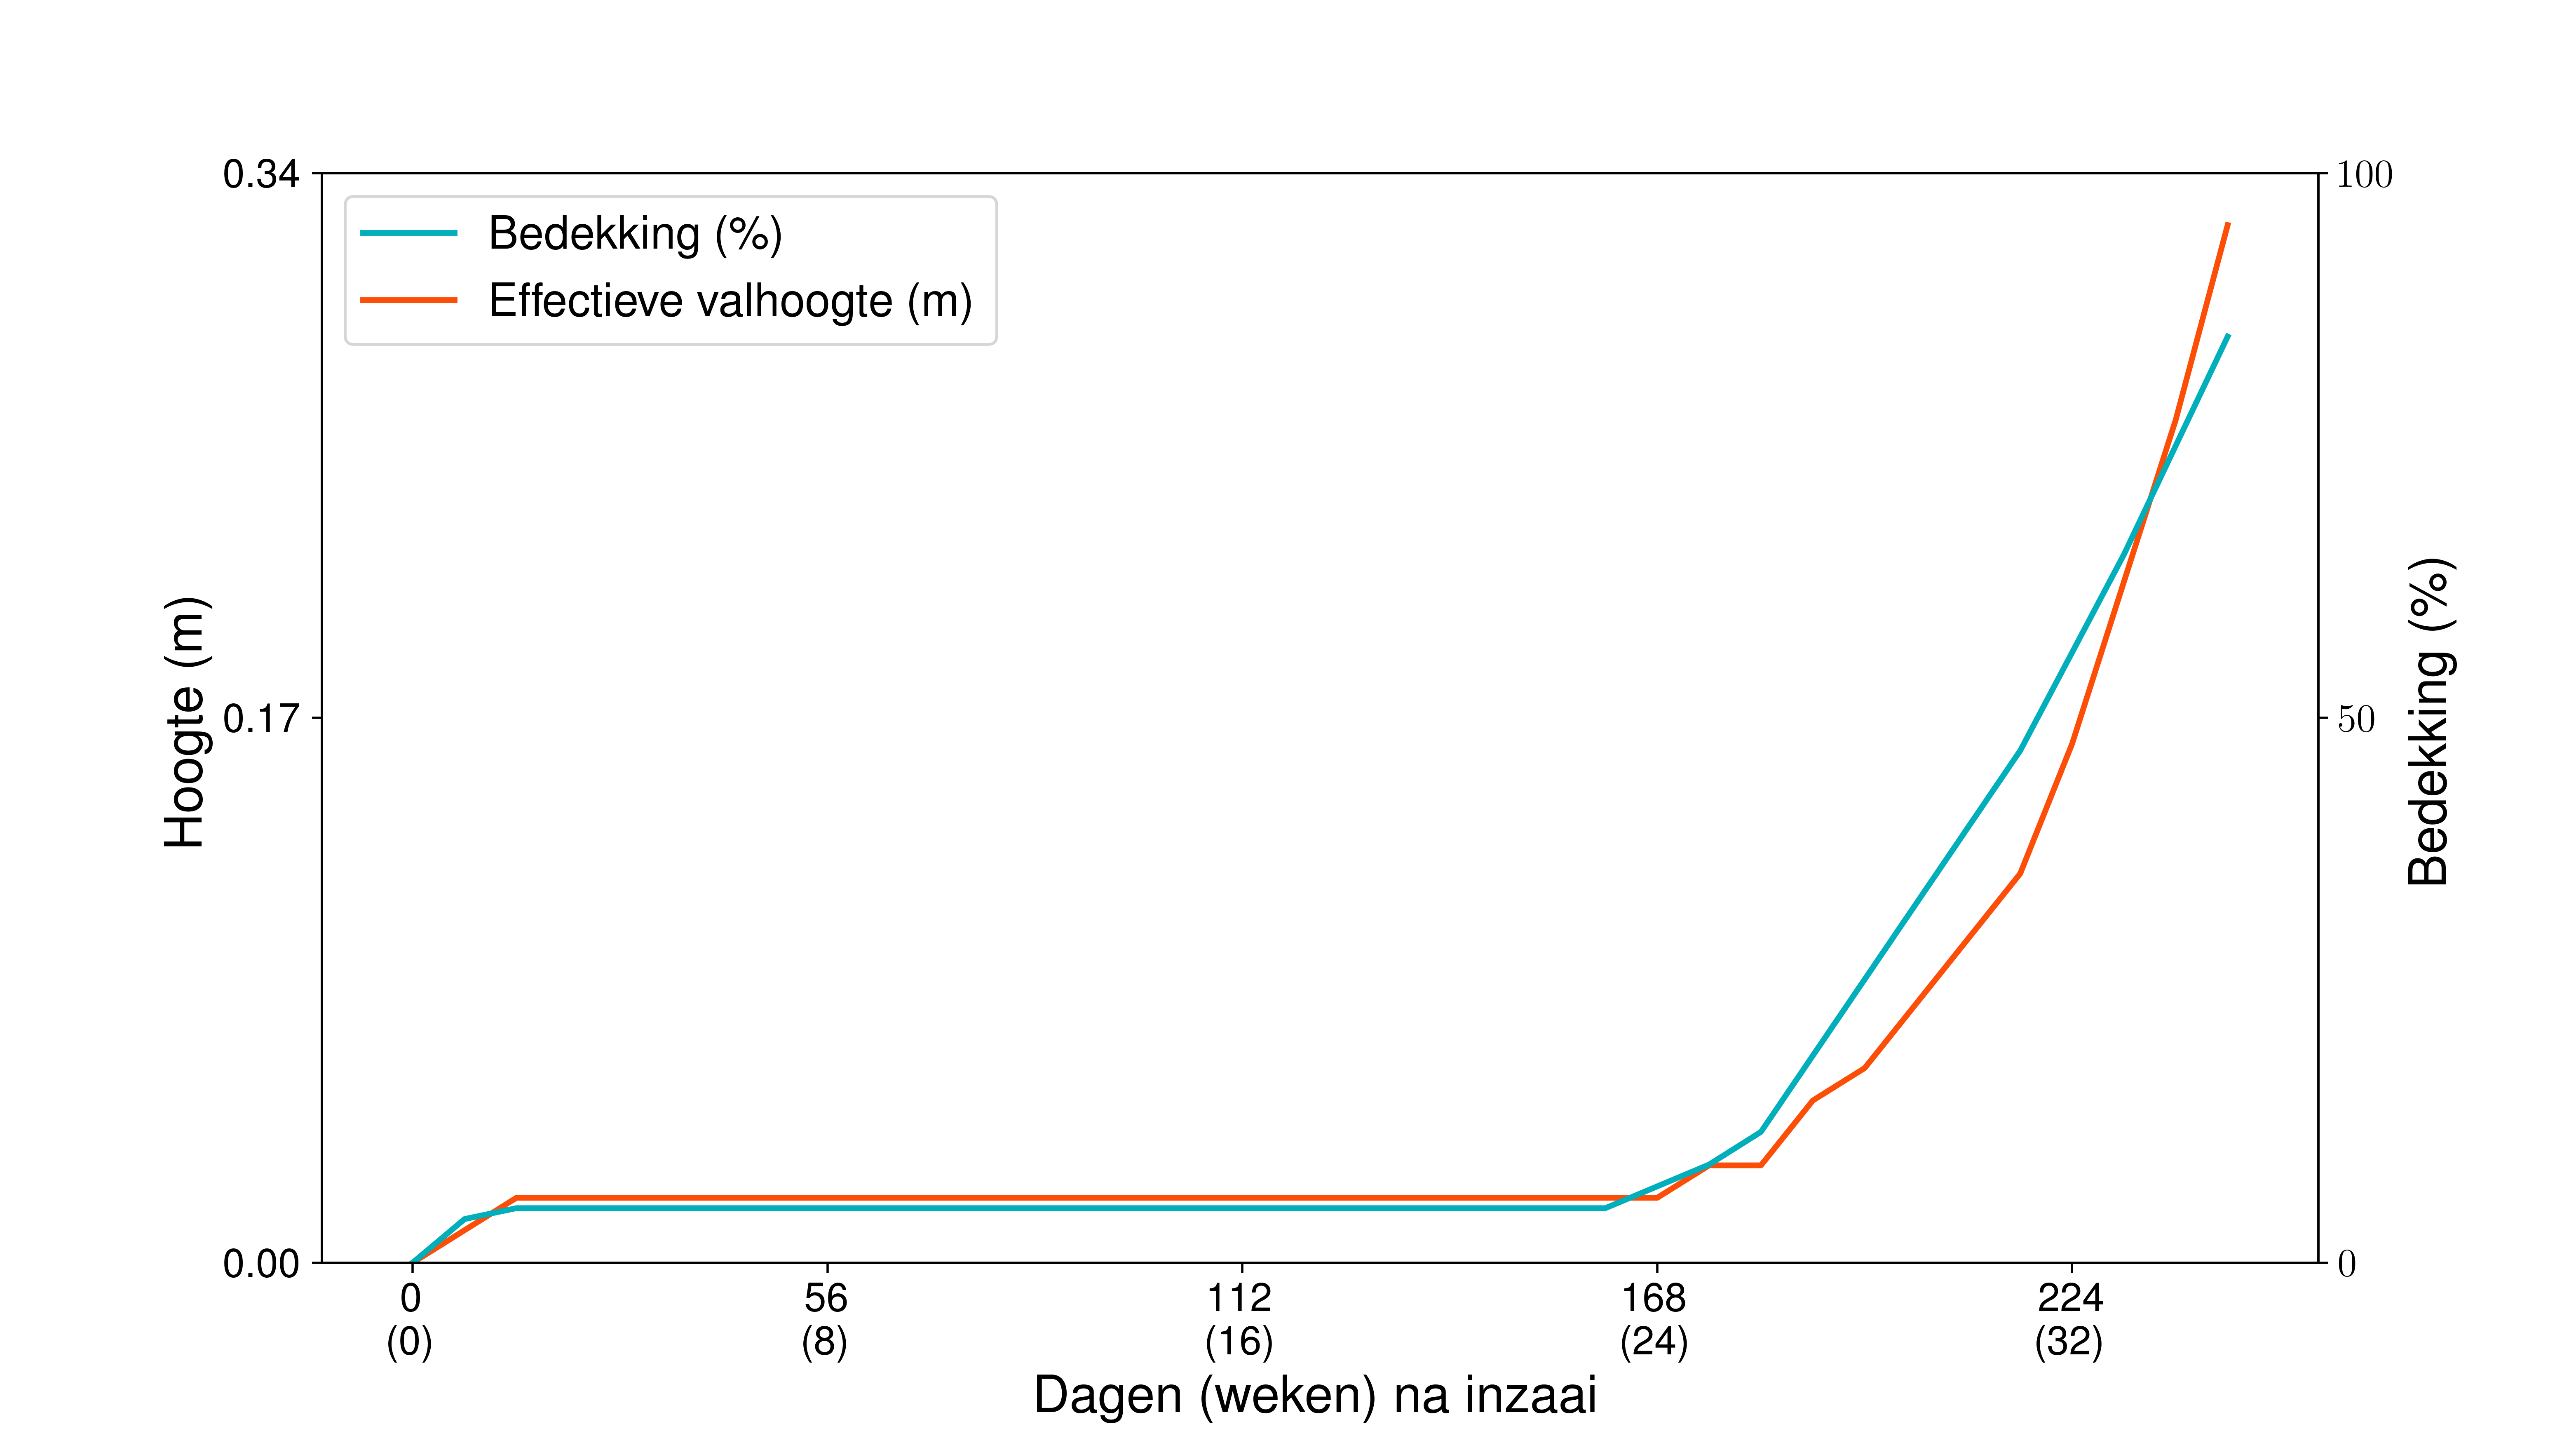
\includegraphics[width=12.5cm]{temp/2008.png} \end{figure} \end{center} 
  \textbf{Referenties:} Verbist2004;Gabriels2003;KMI2003;ILVO2019;Gobin2013 \vspace{0.10cm} \\ 
  \textbf{Opmerkingen?} geen \vspace{0.10cm} \\ 
 \newpage 
 \section{Wintergerst (groep\_id 9)} 
 \textbf{Van toepassing op gewasnamen (en codes):} Wintergerst (321) 
 \begin{multicols}{3} \begin{itemize} \item[$\square$] Meerjarig \item[$\square$] Groenbedekker \item[$\square$] Groente \end{itemize} \end{multicols} 
 \subsection{Hoofdteelt, voorteelt en nateelt (inzaaidatum=[0915,1015]) (subgroep\_id 1009)} 
  \textbf{Zaaidatum (dd/mm)}: 15/09  \vspace{0.10cm} \\ 
  \textbf{Oogstdatum (dd/mm)}: 15/07  \vspace{0.10cm} \\ 
  \textbf{Oogstresten} \vspace{0.05cm} \\ 
  \tab Initi\"{e}le hoeveelheid (kg ha$^{-1}$): 3600.00 \vspace{0.05cm} \\ 
  \tab Afbraakcoefficient (-): 0.01 \vspace{0.05cm} \\ 
  \tab Bodembedekking (m$^2$ kg$^{-1}$): 1.20 \vspace{0.05cm} \\ 
  \tab Initieel percentage bedekking (\%): 100 \vspace{0.05cm} \\ 
  \tab Halfwaarde tijd (dagen): 30 \vspace{0.05cm} \\ 
  \textbf{Initi\"{e}le bodemruwheid (mm)}: 10.20 \vspace{0.05cm} \\ 
  \textbf{Gewasgroeicurve subgroep\_id 1009:} 
 \begin{center} \begin{figure}[H] 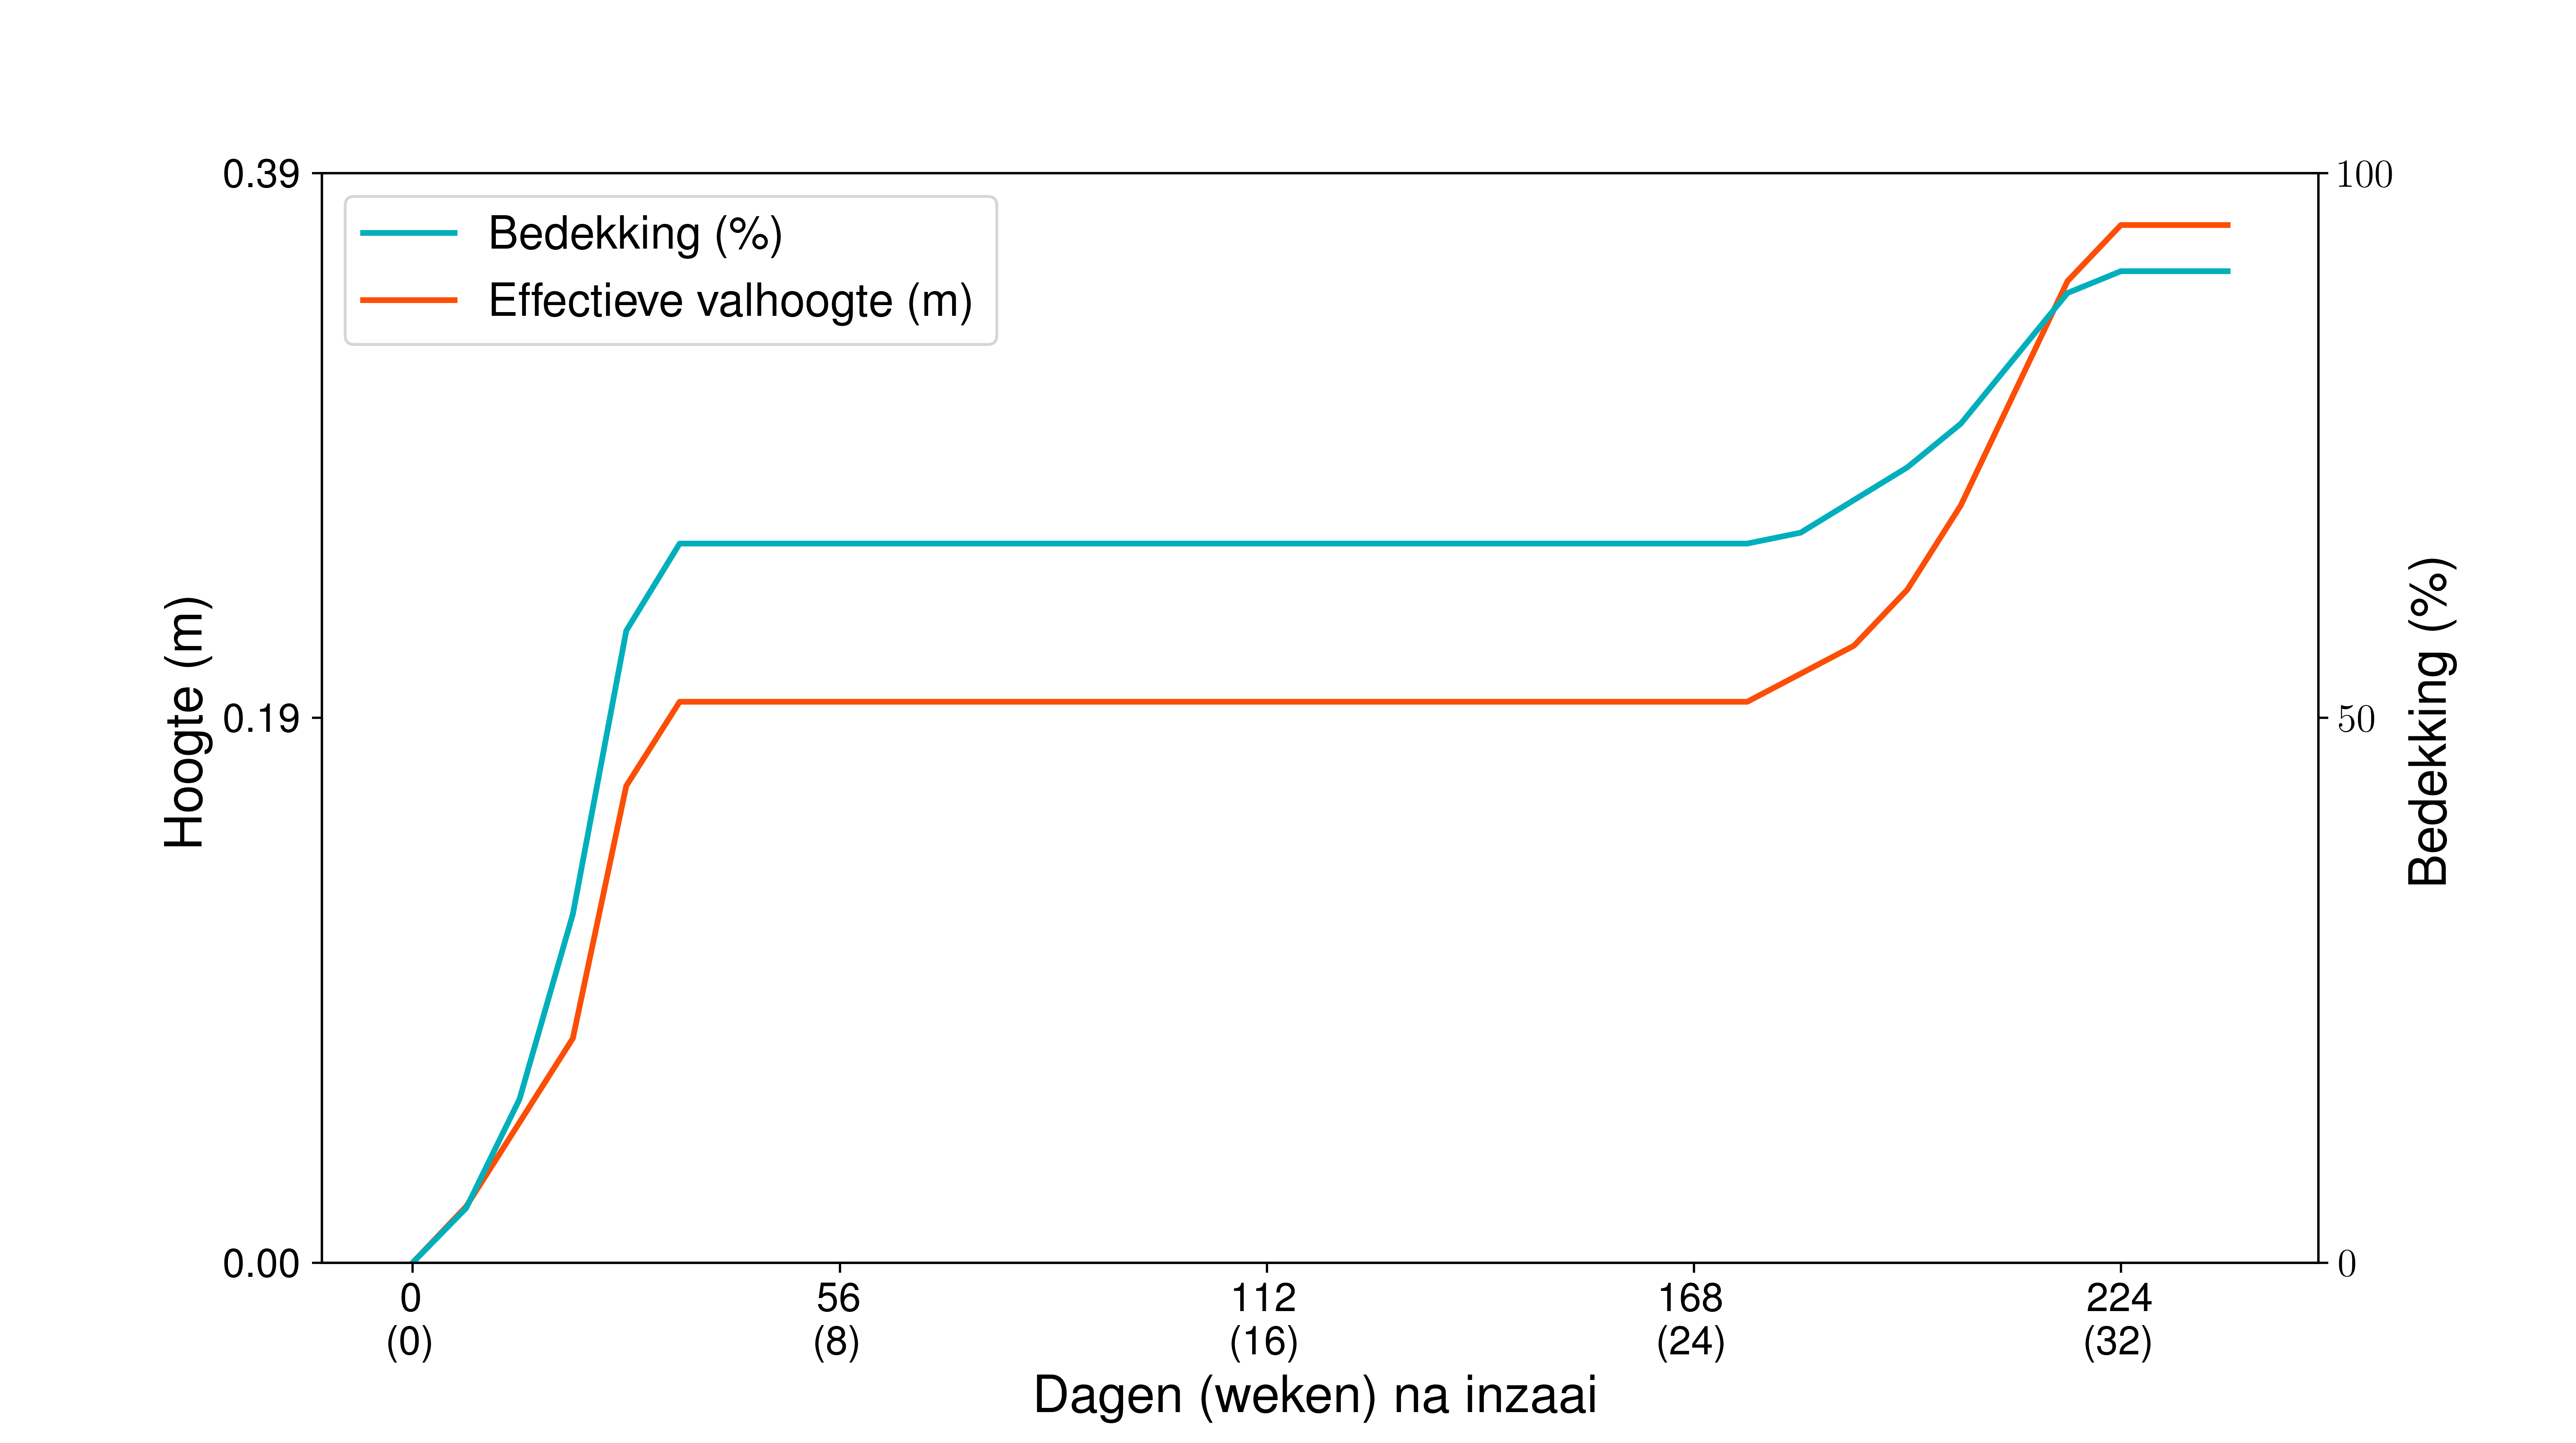
\includegraphics[width=12.5cm]{temp/1009.png} \end{figure} \end{center} 
  \textbf{Referenties:} Verbist2004;Gabriels2003;KMI2003;ILVO2019;Gobin2013 \vspace{0.10cm} \\ 
  \textbf{Opmerkingen?} geen \vspace{0.10cm} \\ 
 \newpage 
 \subsection{Hoofdteelt, voorteelt en nateelt (inzaaidatum=[1015,1030]) (subgroep\_id 1008)} 
  \textbf{Zaaidatum (dd/mm)}: 15/10  \vspace{0.10cm} \\ 
  \textbf{Oogstdatum (dd/mm)}: 15/07  \vspace{0.10cm} \\ 
  \textbf{Oogstresten} \vspace{0.05cm} \\ 
  \tab Initi\"{e}le hoeveelheid (kg ha$^{-1}$): 3600.00 \vspace{0.05cm} \\ 
  \tab Afbraakcoefficient (-): 0.01 \vspace{0.05cm} \\ 
  \tab Bodembedekking (m$^2$ kg$^{-1}$): 1.20 \vspace{0.05cm} \\ 
  \tab Initieel percentage bedekking (\%): 100 \vspace{0.05cm} \\ 
  \tab Halfwaarde tijd (dagen): 30 \vspace{0.05cm} \\ 
  \textbf{Initi\"{e}le bodemruwheid (mm)}: 10.20 \vspace{0.05cm} \\ 
  \textbf{Gewasgroeicurve subgroep\_id 1008:} 
 \begin{center} \begin{figure}[H] 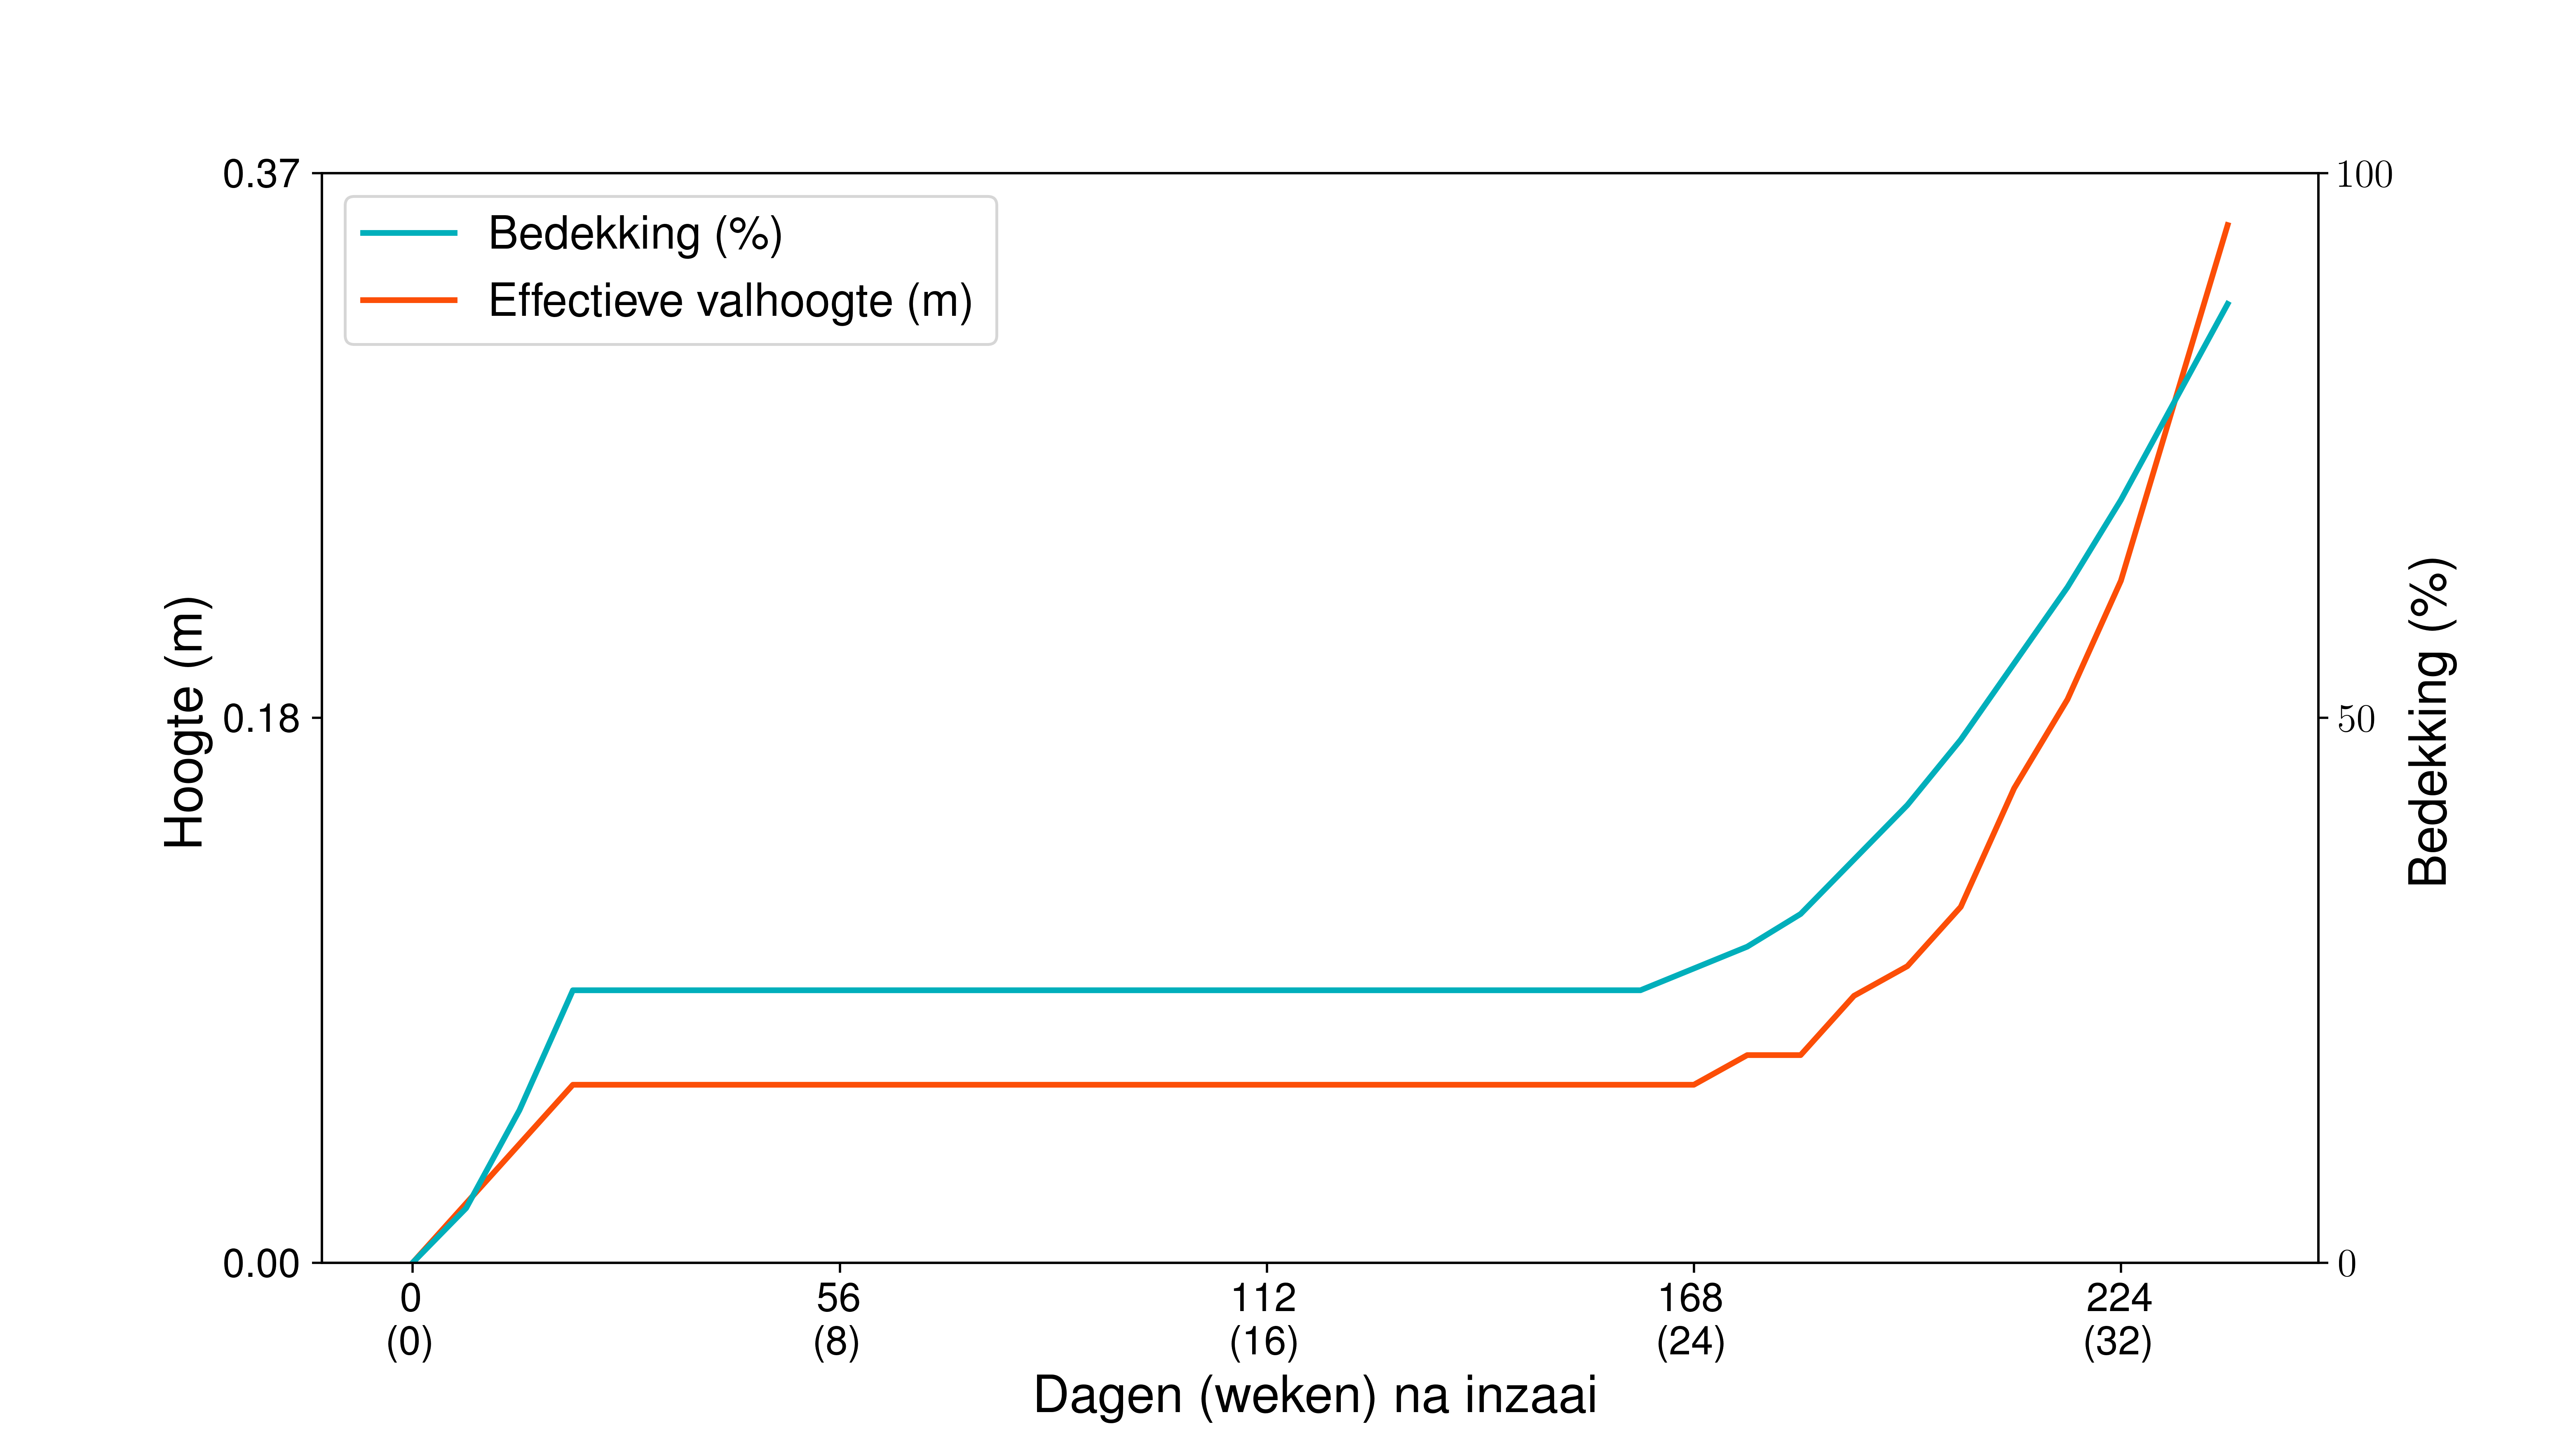
\includegraphics[width=12.5cm]{temp/1008.png} \end{figure} \end{center} 
  \textbf{Referenties:} Verbist2004;Gabriels2003;KMI2003;ILVO2019;Gobin2013 \vspace{0.10cm} \\ 
  \textbf{Opmerkingen?} geen \vspace{0.10cm} \\ 
 \newpage 
 \subsection{Hoofdteelt, voorteelt en nateelt (inzaaidatum=[1030,1231]) (subgroep\_id 2008)} 
  \textbf{Zaaidatum (dd/mm)}: 30/10  \vspace{0.10cm} \\ 
  \textbf{Oogstdatum (dd/mm)}: 15/07  \vspace{0.10cm} \\ 
  \textbf{Oogstresten} \vspace{0.05cm} \\ 
  \tab Initi\"{e}le hoeveelheid (kg ha$^{-1}$): 3600.00 \vspace{0.05cm} \\ 
  \tab Afbraakcoefficient (-): 0.01 \vspace{0.05cm} \\ 
  \tab Bodembedekking (m$^2$ kg$^{-1}$): 1.20 \vspace{0.05cm} \\ 
  \tab Initieel percentage bedekking (\%): 100 \vspace{0.05cm} \\ 
  \tab Halfwaarde tijd (dagen): 30 \vspace{0.05cm} \\ 
  \textbf{Initi\"{e}le bodemruwheid (mm)}: 10.20 \vspace{0.05cm} \\ 
  \textbf{Gewasgroeicurve subgroep\_id 2008:} 
 \begin{center} \begin{figure}[H] 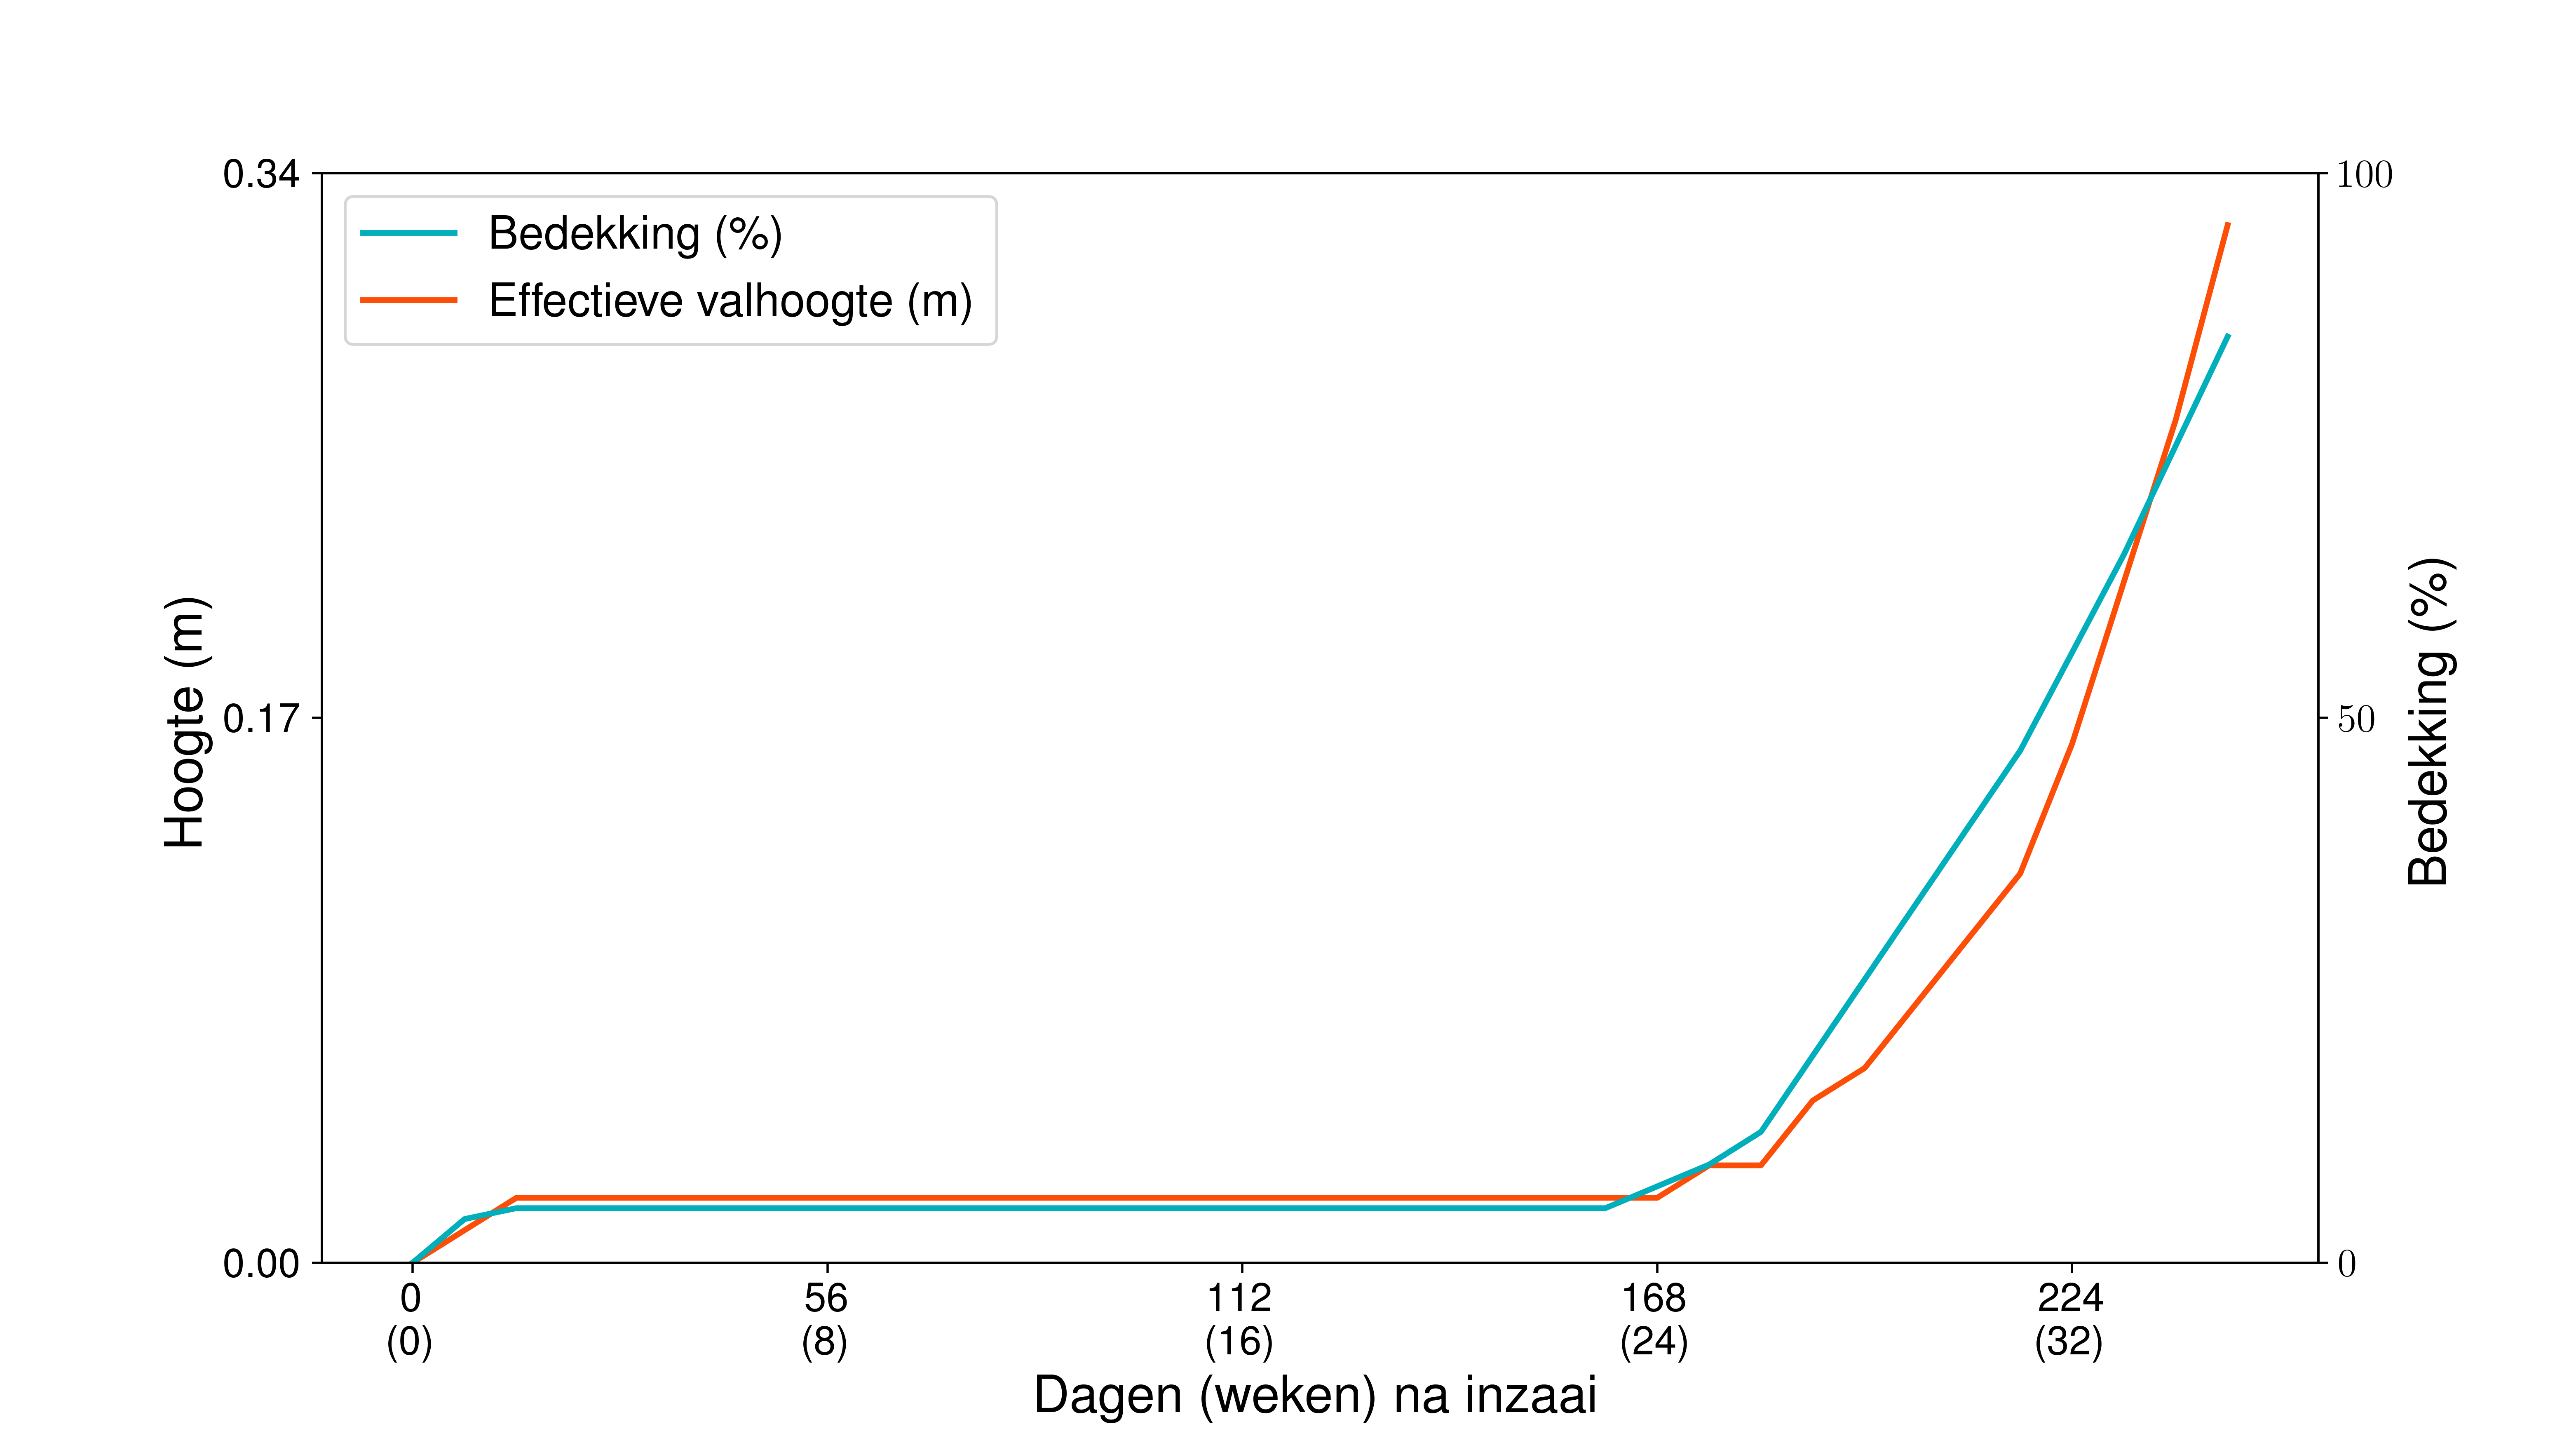
\includegraphics[width=12.5cm]{temp/2008.png} \end{figure} \end{center} 
  \textbf{Referenties:} Verbist2004;Gabriels2003;KMI2003;ILVO2019;Gobin2013 \vspace{0.10cm} \\ 
  \textbf{Opmerkingen?} geen \vspace{0.10cm} \\ 
 \newpage 
 \section{Zomertarwe (groep\_id 11)} 
 \textbf{Van toepassing op gewasnamen (en codes):} Zomertarwe (312) 
 \begin{multicols}{3} \begin{itemize} \item[$\square$] Meerjarig \item[$\square$] Groenbedekker \item[$\square$] Groente \end{itemize} \end{multicols} 
  \textbf{Zaaidatum (dd/mm)}: 15/03  \vspace{0.10cm} \\ 
  \textbf{Oogstdatum (dd/mm)}: 15/08  \vspace{0.10cm} \\ 
  \textbf{Oogstresten} \vspace{0.05cm} \\ 
  \tab Initi\"{e}le hoeveelheid (kg ha$^{-1}$): 3600.00 \vspace{0.05cm} \\ 
  \tab Afbraakcoefficient (-): 0.01 \vspace{0.05cm} \\ 
  \tab Bodembedekking (m$^2$ kg$^{-1}$): 1.20 \vspace{0.05cm} \\ 
  \tab Initieel percentage bedekking (\%): 100 \vspace{0.05cm} \\ 
  \tab Halfwaarde tijd (dagen): 30 \vspace{0.05cm} \\ 
  \textbf{Initi\"{e}le bodemruwheid (mm)}: 10.20 \vspace{0.05cm} \\ 
  \textbf{Gewasgroeicurve subgroep\_id 1010:} 
 \begin{center} \begin{figure}[H] 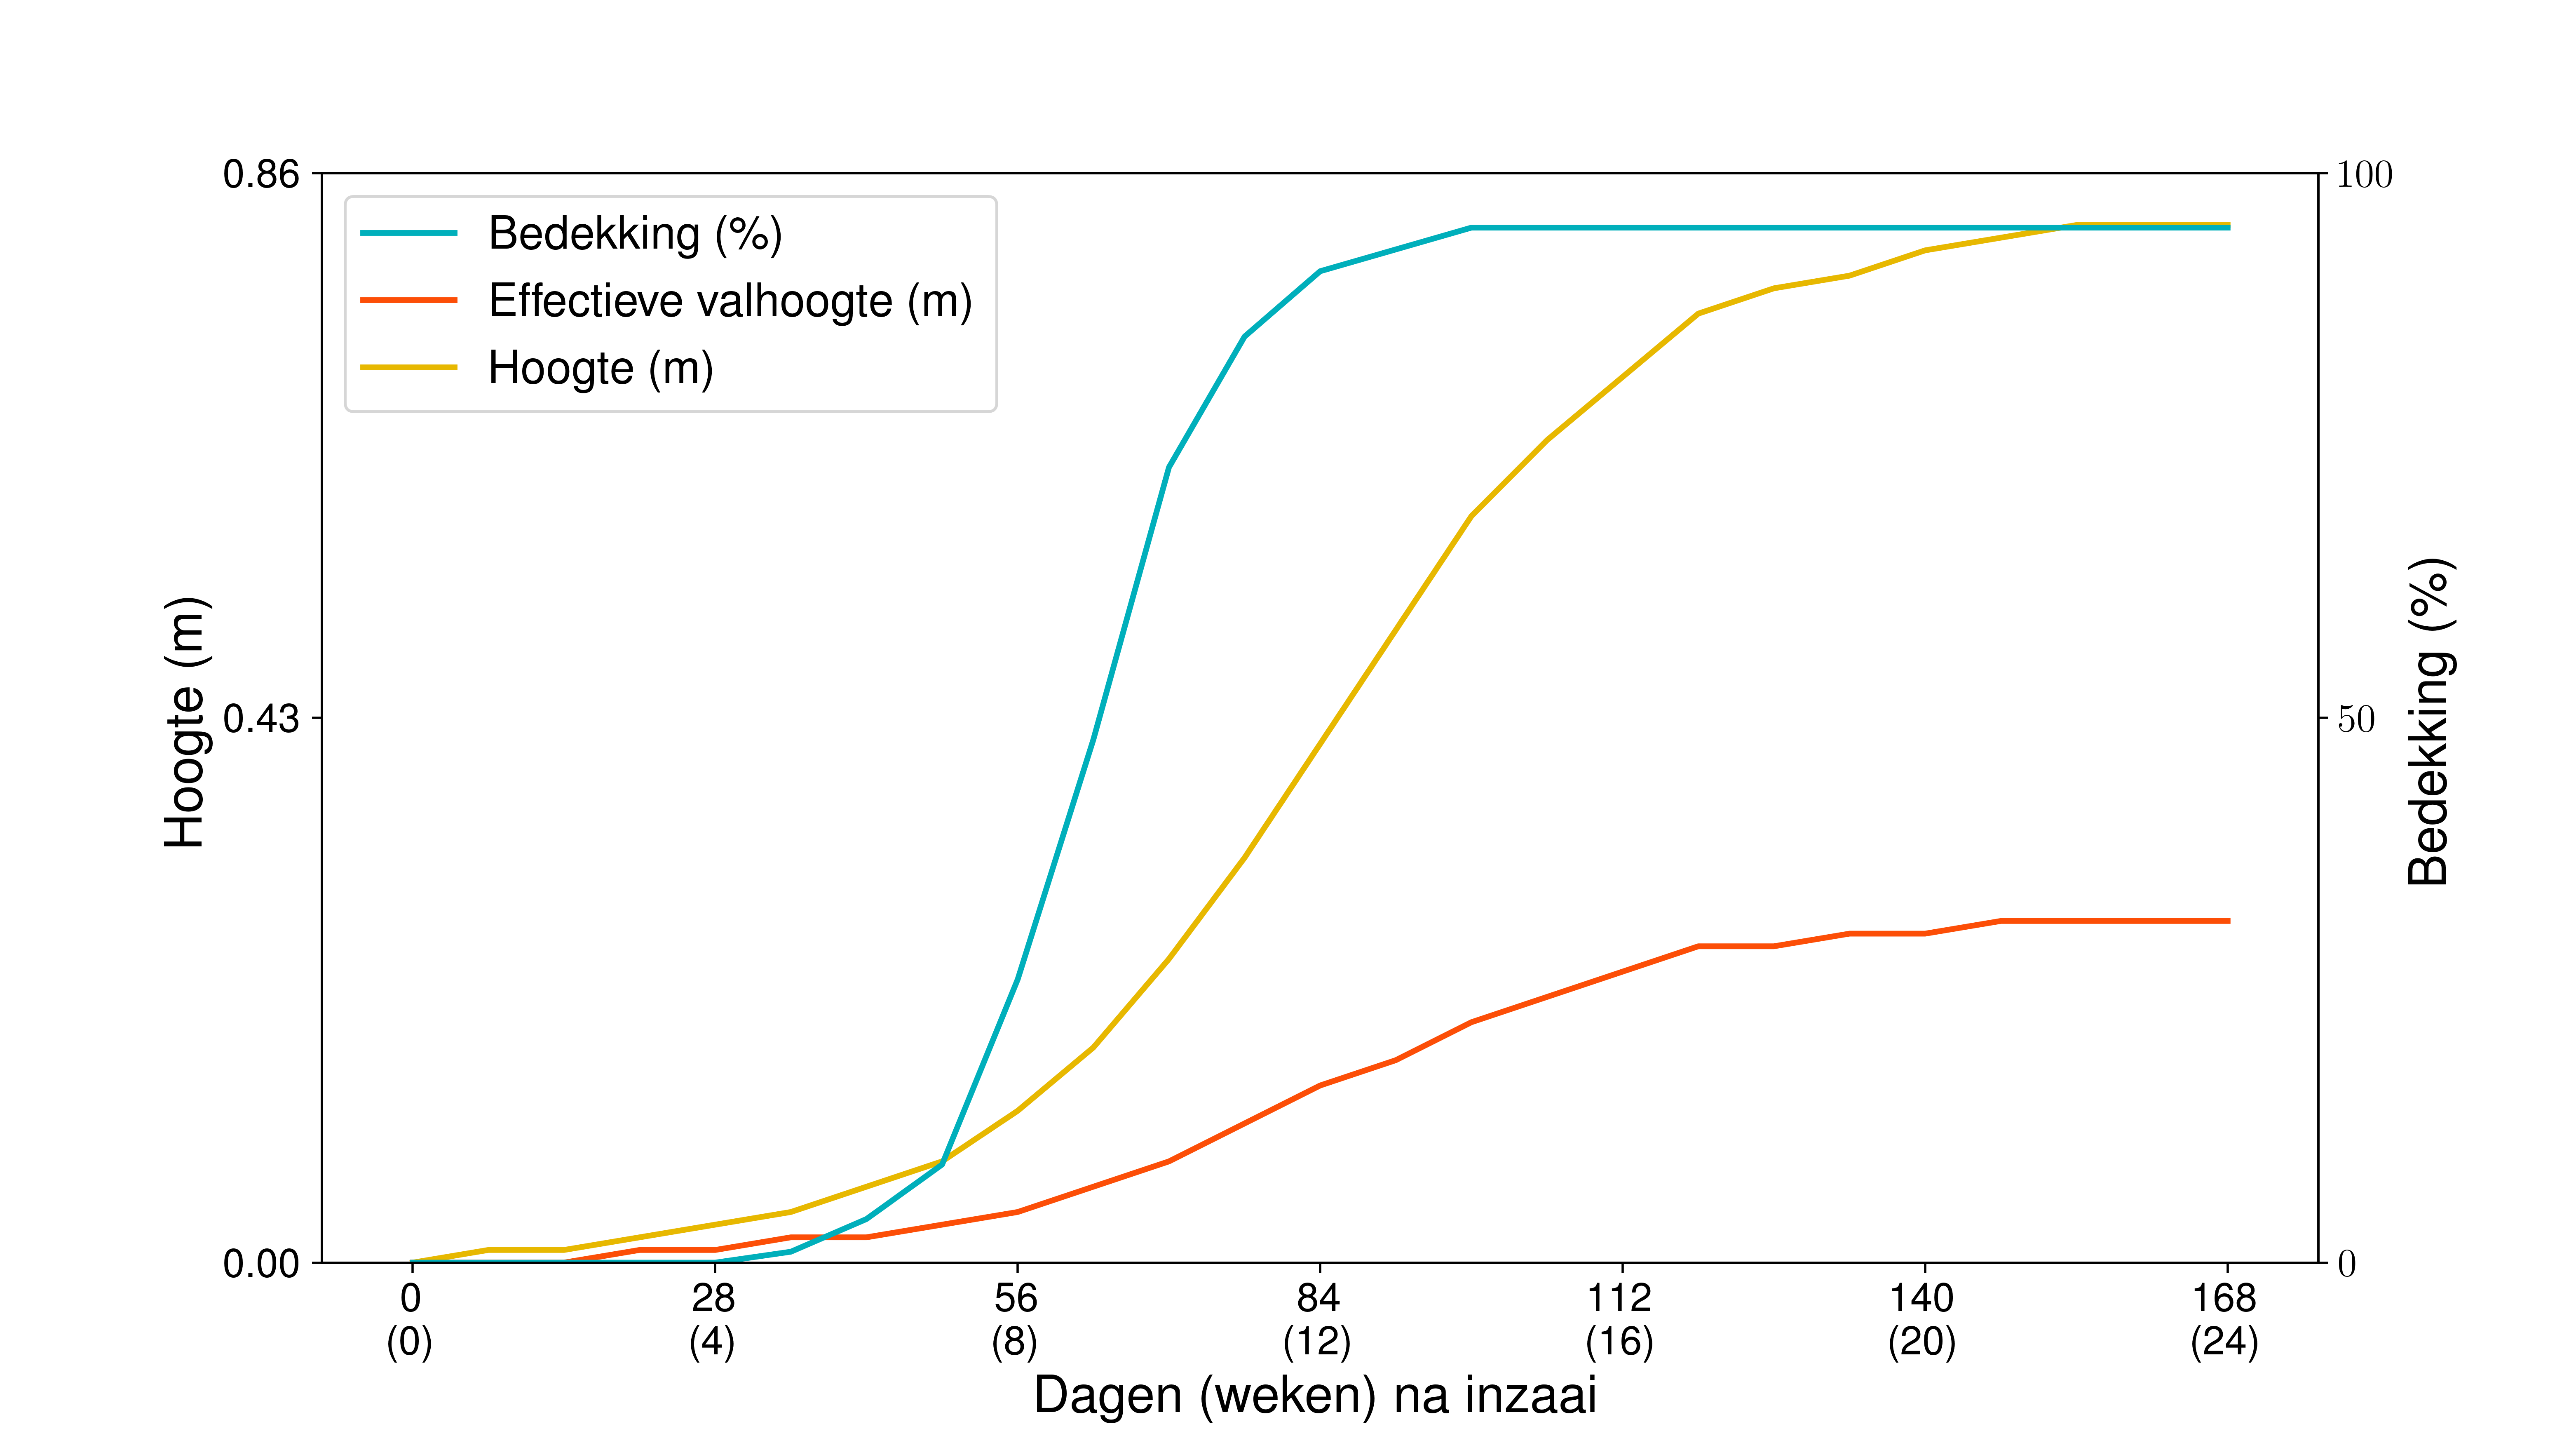
\includegraphics[width=12.5cm]{temp/1010.png} \end{figure} \end{center} 
  \textbf{Referenties:} Verbist2004;Gabriels2003;KMI2003;ILVO2019;Gobin2013 \vspace{0.10cm} \\ 
  \textbf{Opmerkingen?} geen \vspace{0.10cm} \\ 
 \newpage 
 \section{Zomergerst (groep\_id 12)} 
 \textbf{Van toepassing op gewasnamen (en codes):} Zomergerst (322) 
 \begin{multicols}{3} \begin{itemize} \item[$\square$] Meerjarig \item[$\square$] Groenbedekker \item[$\square$] Groente \end{itemize} \end{multicols} 
  \textbf{Zaaidatum (dd/mm)}: 15/03  \vspace{0.10cm} \\ 
  \textbf{Oogstdatum (dd/mm)}: 01/08  \vspace{0.10cm} \\ 
  \textbf{Oogstresten} \vspace{0.05cm} \\ 
  \tab Initi\"{e}le hoeveelheid (kg ha$^{-1}$): 3600.00 \vspace{0.05cm} \\ 
  \tab Afbraakcoefficient (-): 0.01 \vspace{0.05cm} \\ 
  \tab Bodembedekking (m$^2$ kg$^{-1}$): 1.20 \vspace{0.05cm} \\ 
  \tab Initieel percentage bedekking (\%): 100 \vspace{0.05cm} \\ 
  \tab Halfwaarde tijd (dagen): 30 \vspace{0.05cm} \\ 
  \textbf{Initi\"{e}le bodemruwheid (mm)}: 10.20 \vspace{0.05cm} \\ 
  \textbf{Gewasgroeicurve subgroep\_id 1010:} 
 \begin{center} \begin{figure}[H] 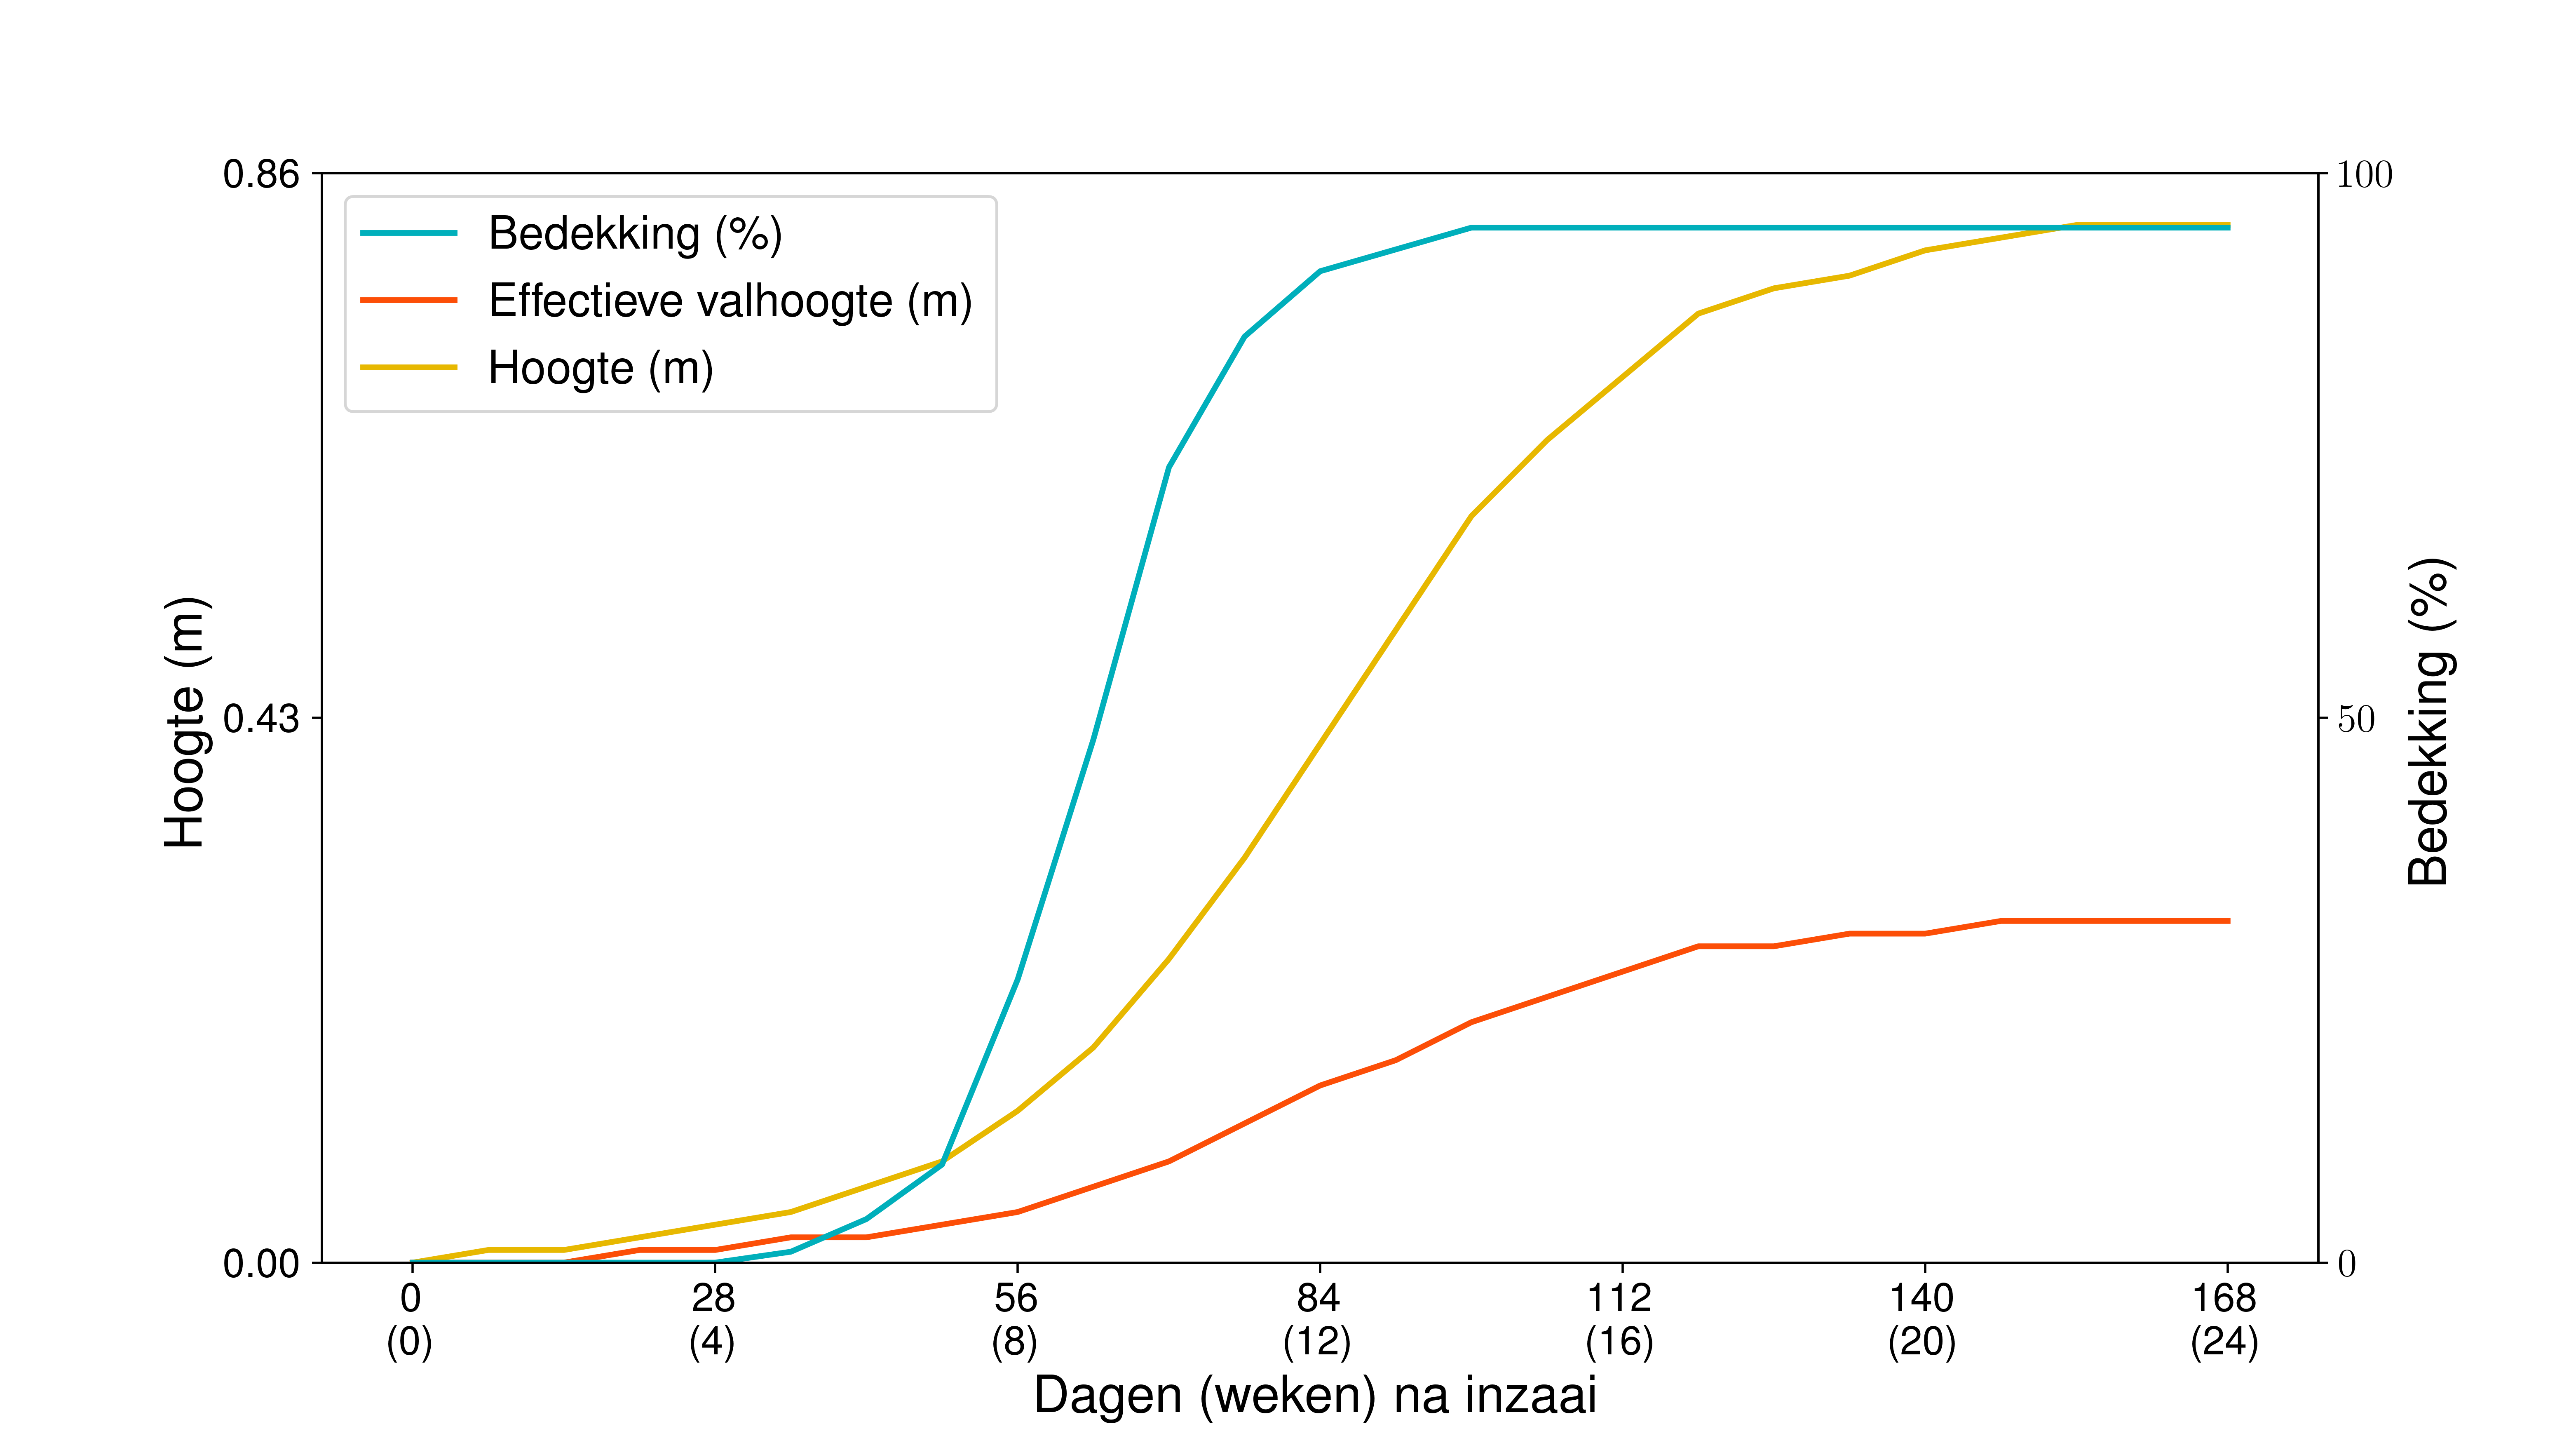
\includegraphics[width=12.5cm]{temp/1010.png} \end{figure} \end{center} 
  \textbf{Referenties:} Verbist2004;Gabriels2003;KMI2003;ILVO2019;Gobin2013 \vspace{0.10cm} \\ 
  \textbf{Opmerkingen?} geen \vspace{0.10cm} \\ 
 \newpage 
 \section{Brouwgerst (groep\_id 10)} 
 \textbf{Van toepassing op gewasnamen (en codes):} Brouwgerst (323) 
 \begin{multicols}{3} \begin{itemize} \item[$\square$] Meerjarig \item[$\square$] Groenbedekker \item[$\square$] Groente \end{itemize} \end{multicols} 
 \subsection{Nateelt (inzaaidatum=[0915,1015]) (subgroep\_id 1009)} 
  \textbf{Zaaidatum (dd/mm)}: 15/09  \vspace{0.10cm} \\ 
  \textbf{Oogstdatum (dd/mm)}: 15/07  \vspace{0.10cm} \\ 
  \textbf{Oogstresten} \vspace{0.05cm} \\ 
  \tab Initi\"{e}le hoeveelheid (kg ha$^{-1}$): 3600.00 \vspace{0.05cm} \\ 
  \tab Afbraakcoefficient (-): 0.01 \vspace{0.05cm} \\ 
  \tab Bodembedekking (m$^2$ kg$^{-1}$): 1.20 \vspace{0.05cm} \\ 
  \tab Initieel percentage bedekking (\%): 100 \vspace{0.05cm} \\ 
  \tab Halfwaarde tijd (dagen): 30 \vspace{0.05cm} \\ 
  \textbf{Initi\"{e}le bodemruwheid (mm)}: 10.20 \vspace{0.05cm} \\ 
  \textbf{Gewasgroeicurve subgroep\_id 1009:} 
 \begin{center} \begin{figure}[H] 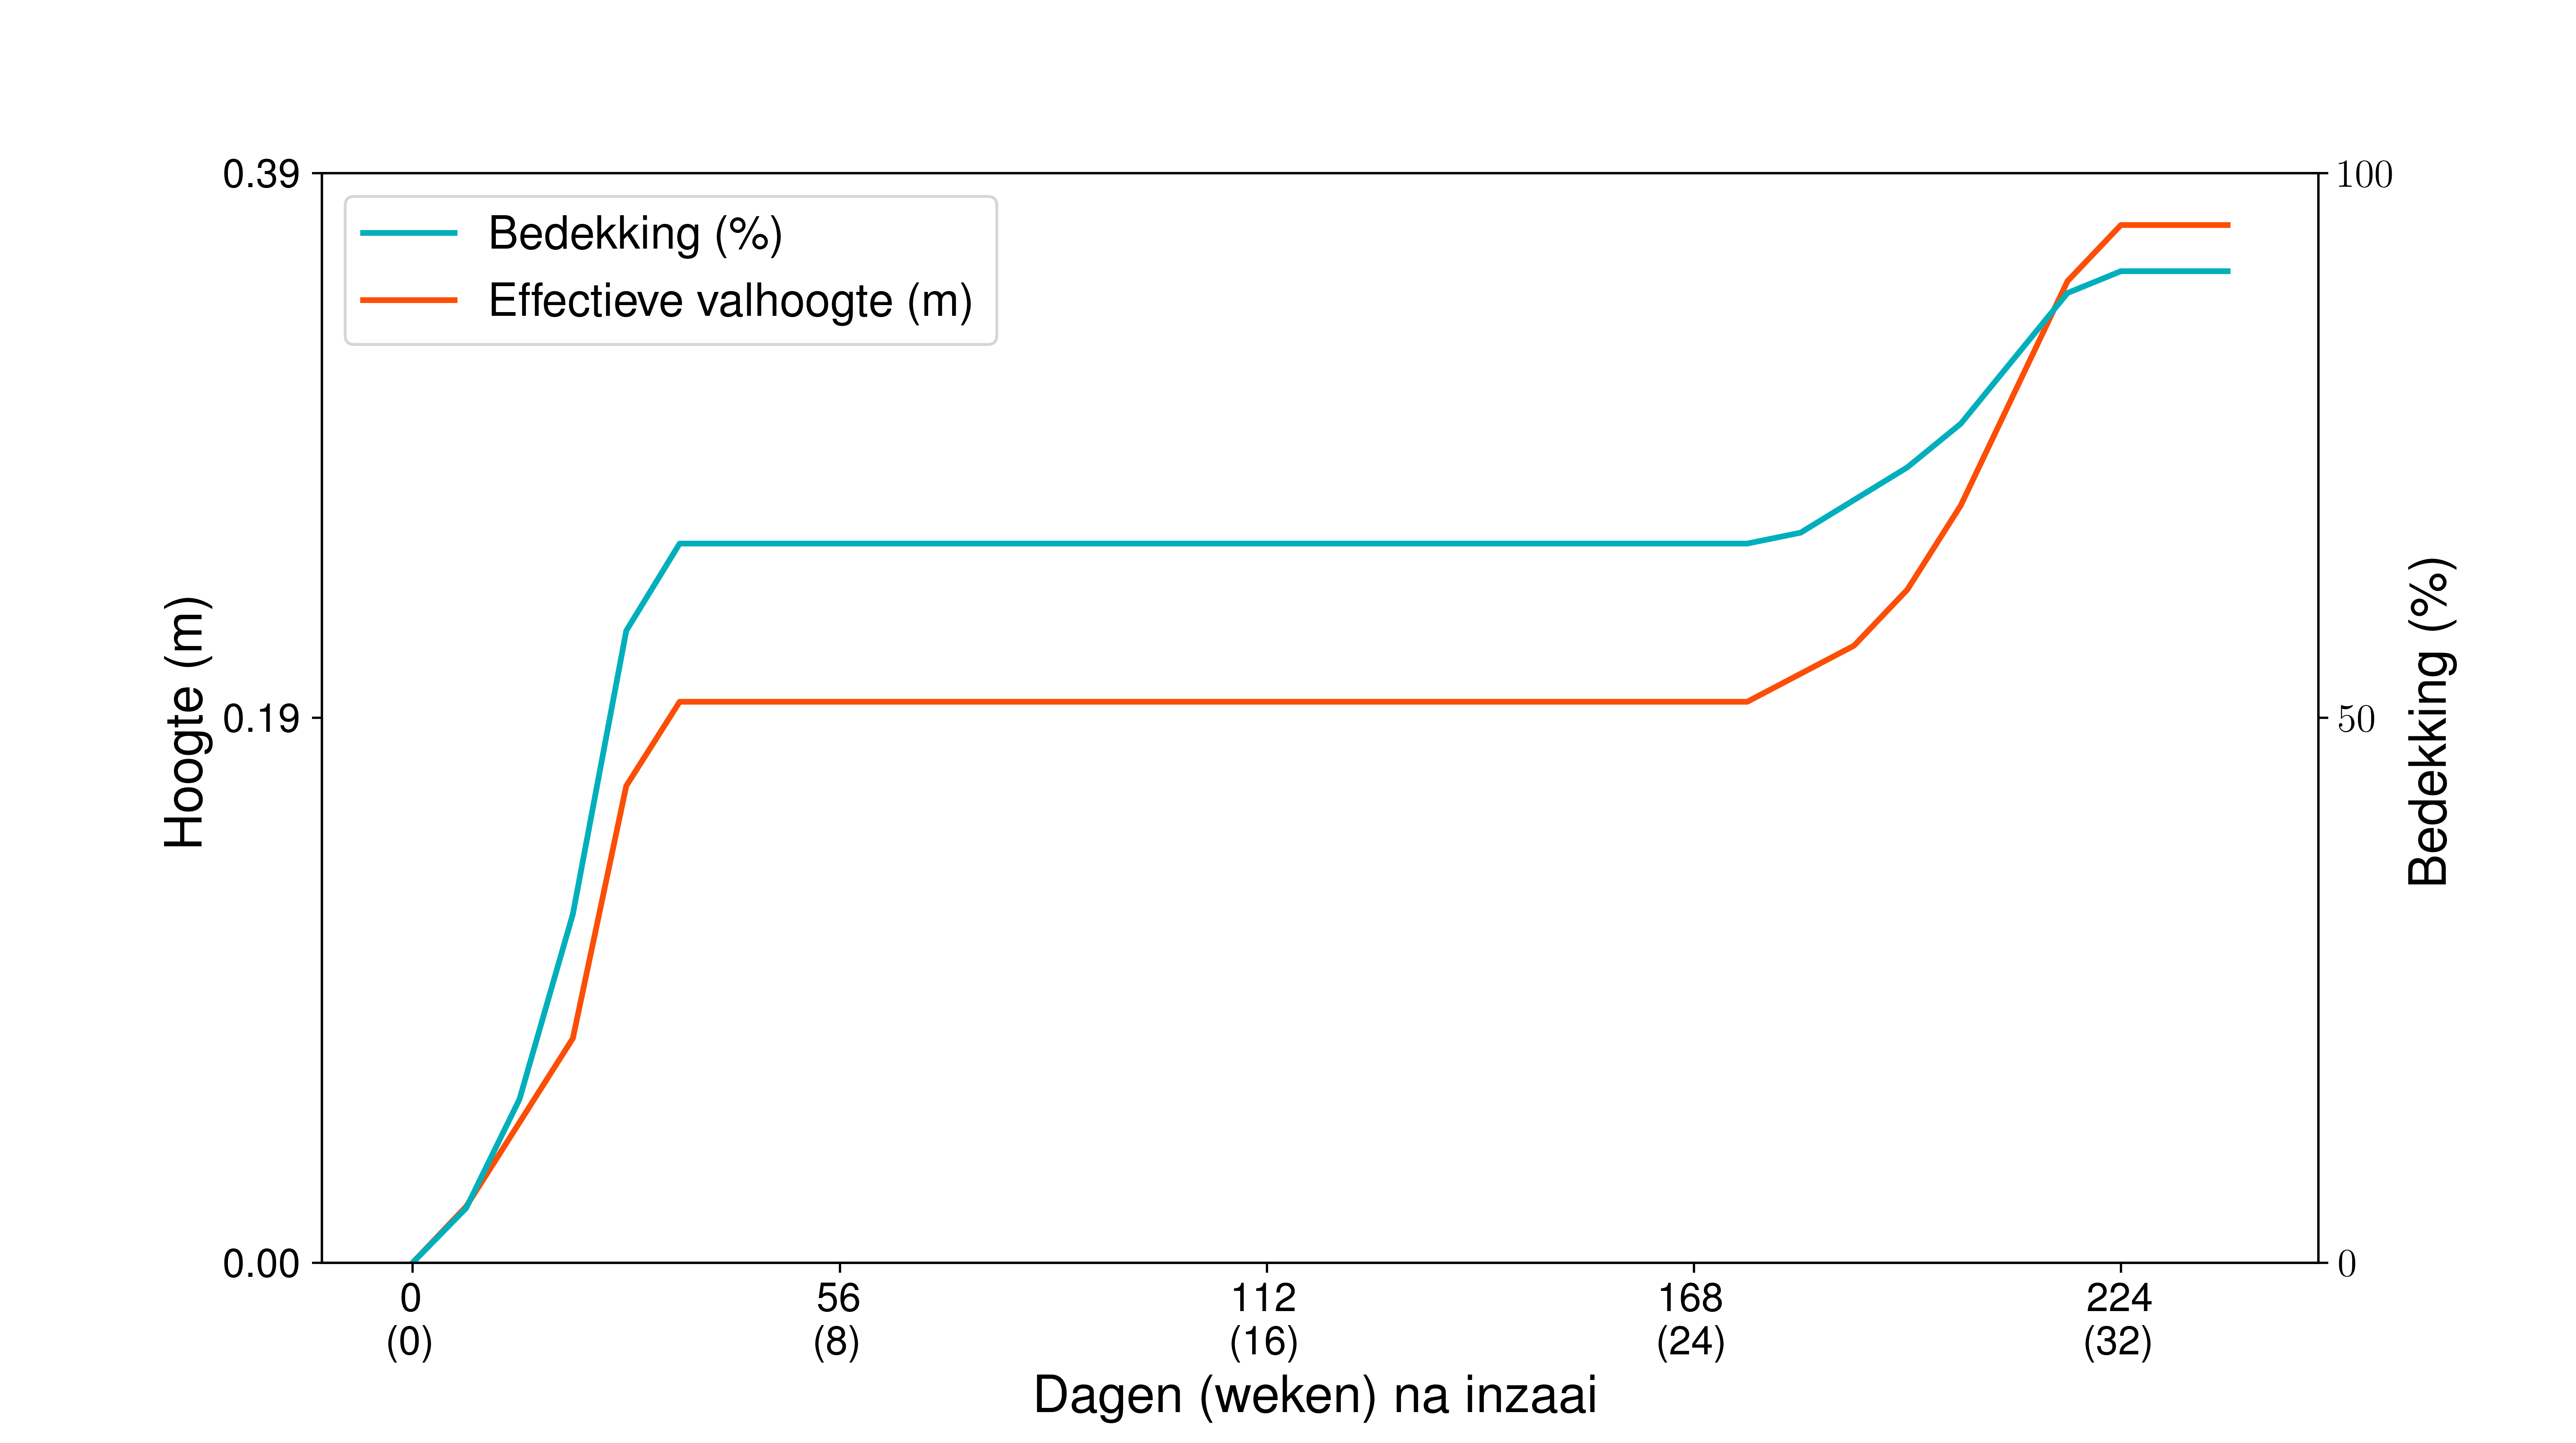
\includegraphics[width=12.5cm]{temp/1009.png} \end{figure} \end{center} 
  \textbf{Referenties:} Verbist2004;Gabriels2003;KMI2003;ILVO2019;Gobin2013 \vspace{0.10cm} \\ 
  \textbf{Opmerkingen?} overerving wintergerst: (Als er nateelt(jaar i-1) == brouwersgerst en-of voorteelt (jaar i)== brouwersgerst ) en hoofdteelt (jaar i) == brouwersgerst \vspace{0.10cm} \\ 
 \newpage 
 \subsection{Nateelt (inzaaidatum=[1015,1030]) (subgroep\_id 1008)} 
  \textbf{Zaaidatum (dd/mm)}: 15/10  \vspace{0.10cm} \\ 
  \textbf{Oogstdatum (dd/mm)}: 15/07  \vspace{0.10cm} \\ 
  \textbf{Oogstresten} \vspace{0.05cm} \\ 
  \tab Initi\"{e}le hoeveelheid (kg ha$^{-1}$): 3600.00 \vspace{0.05cm} \\ 
  \tab Afbraakcoefficient (-): 0.01 \vspace{0.05cm} \\ 
  \tab Bodembedekking (m$^2$ kg$^{-1}$): 1.20 \vspace{0.05cm} \\ 
  \tab Initieel percentage bedekking (\%): 100 \vspace{0.05cm} \\ 
  \tab Halfwaarde tijd (dagen): 30 \vspace{0.05cm} \\ 
  \textbf{Initi\"{e}le bodemruwheid (mm)}: 10.20 \vspace{0.05cm} \\ 
  \textbf{Gewasgroeicurve subgroep\_id 1008:} 
 \begin{center} \begin{figure}[H] 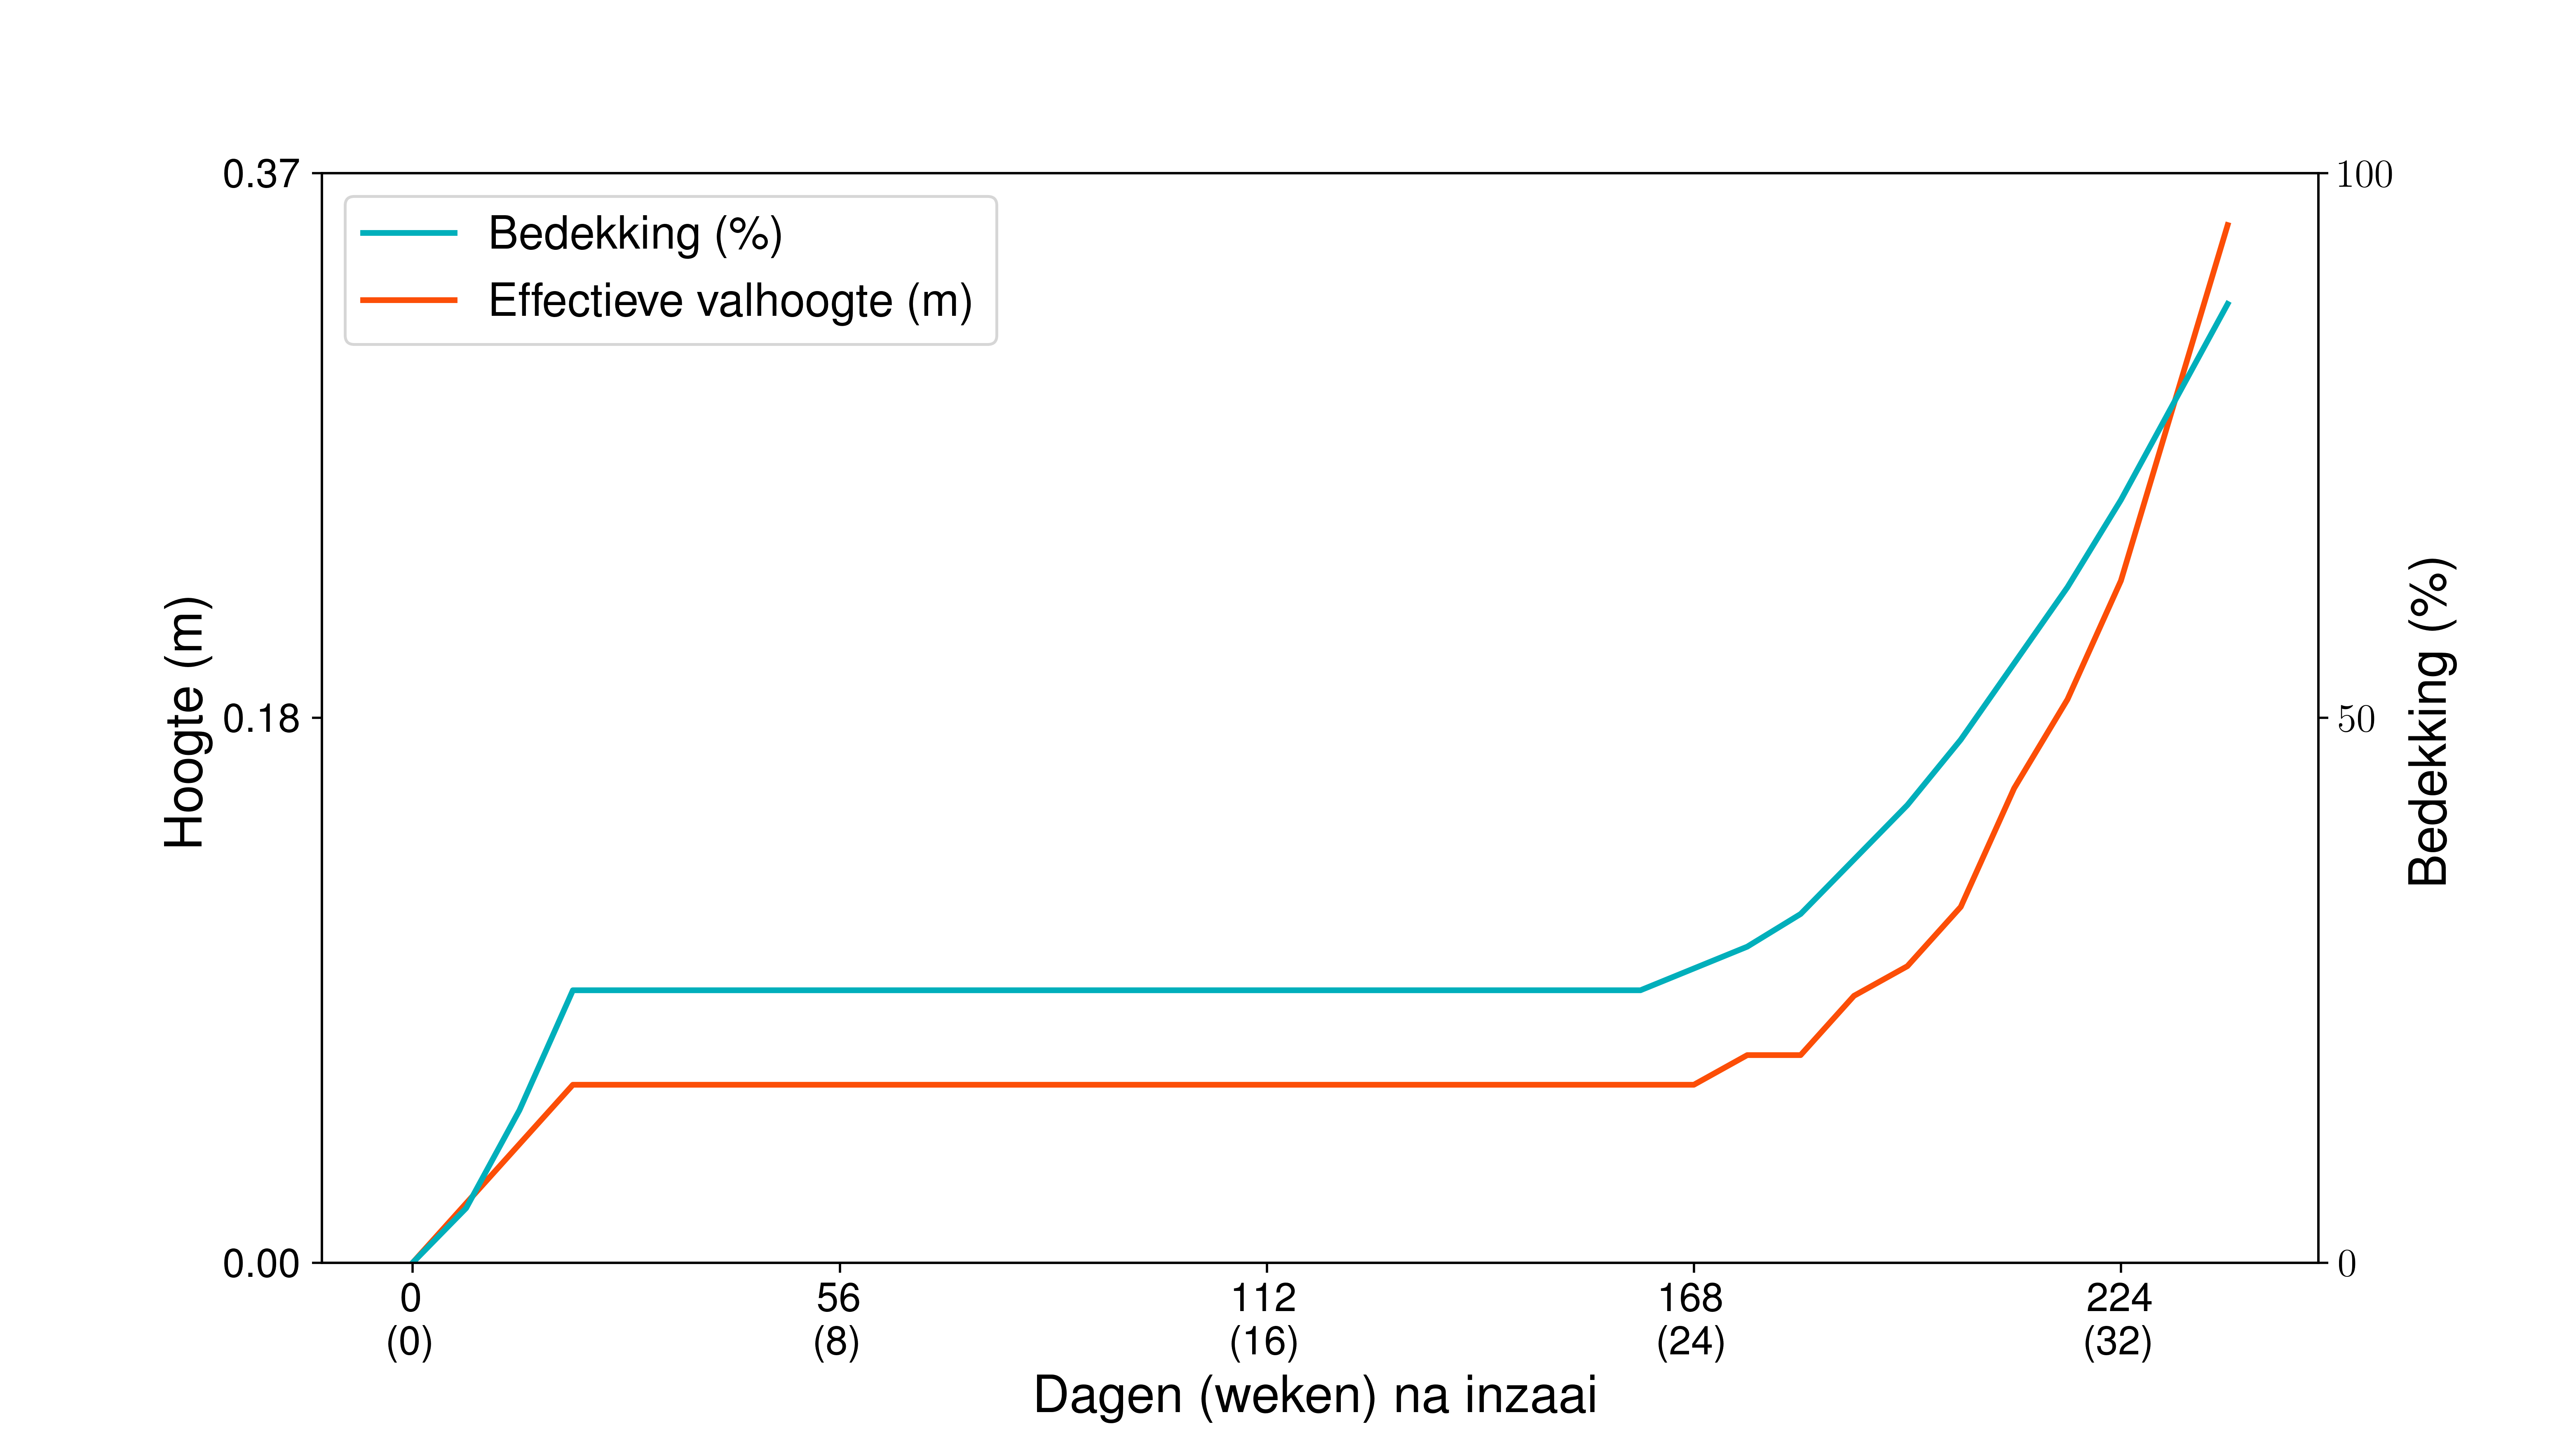
\includegraphics[width=12.5cm]{temp/1008.png} \end{figure} \end{center} 
  \textbf{Referenties:} Verbist2004;Gabriels2003;KMI2003;ILVO2019;Gobin2013 \vspace{0.10cm} \\ 
  \textbf{Opmerkingen?} overerving wintergerst: (Als er nateelt(jaar i-1) == brouwersgerst en-of voorteelt (jaar i)== brouwersgerst ) en hoofdteelt (jaar i) == brouwersgerst \vspace{0.10cm} \\ 
 \newpage 
 \subsection{Nateelt (inzaaidatum=[1030,1231]) (subgroep\_id 2008)} 
  \textbf{Zaaidatum (dd/mm)}: 30/10  \vspace{0.10cm} \\ 
  \textbf{Oogstdatum (dd/mm)}: 15/07  \vspace{0.10cm} \\ 
  \textbf{Oogstresten} \vspace{0.05cm} \\ 
  \tab Initi\"{e}le hoeveelheid (kg ha$^{-1}$): 3600.00 \vspace{0.05cm} \\ 
  \tab Afbraakcoefficient (-): 0.01 \vspace{0.05cm} \\ 
  \tab Bodembedekking (m$^2$ kg$^{-1}$): 1.20 \vspace{0.05cm} \\ 
  \tab Initieel percentage bedekking (\%): 100 \vspace{0.05cm} \\ 
  \tab Halfwaarde tijd (dagen): 30 \vspace{0.05cm} \\ 
  \textbf{Initi\"{e}le bodemruwheid (mm)}: 10.20 \vspace{0.05cm} \\ 
  \textbf{Gewasgroeicurve subgroep\_id 2008:} 
 \begin{center} \begin{figure}[H] 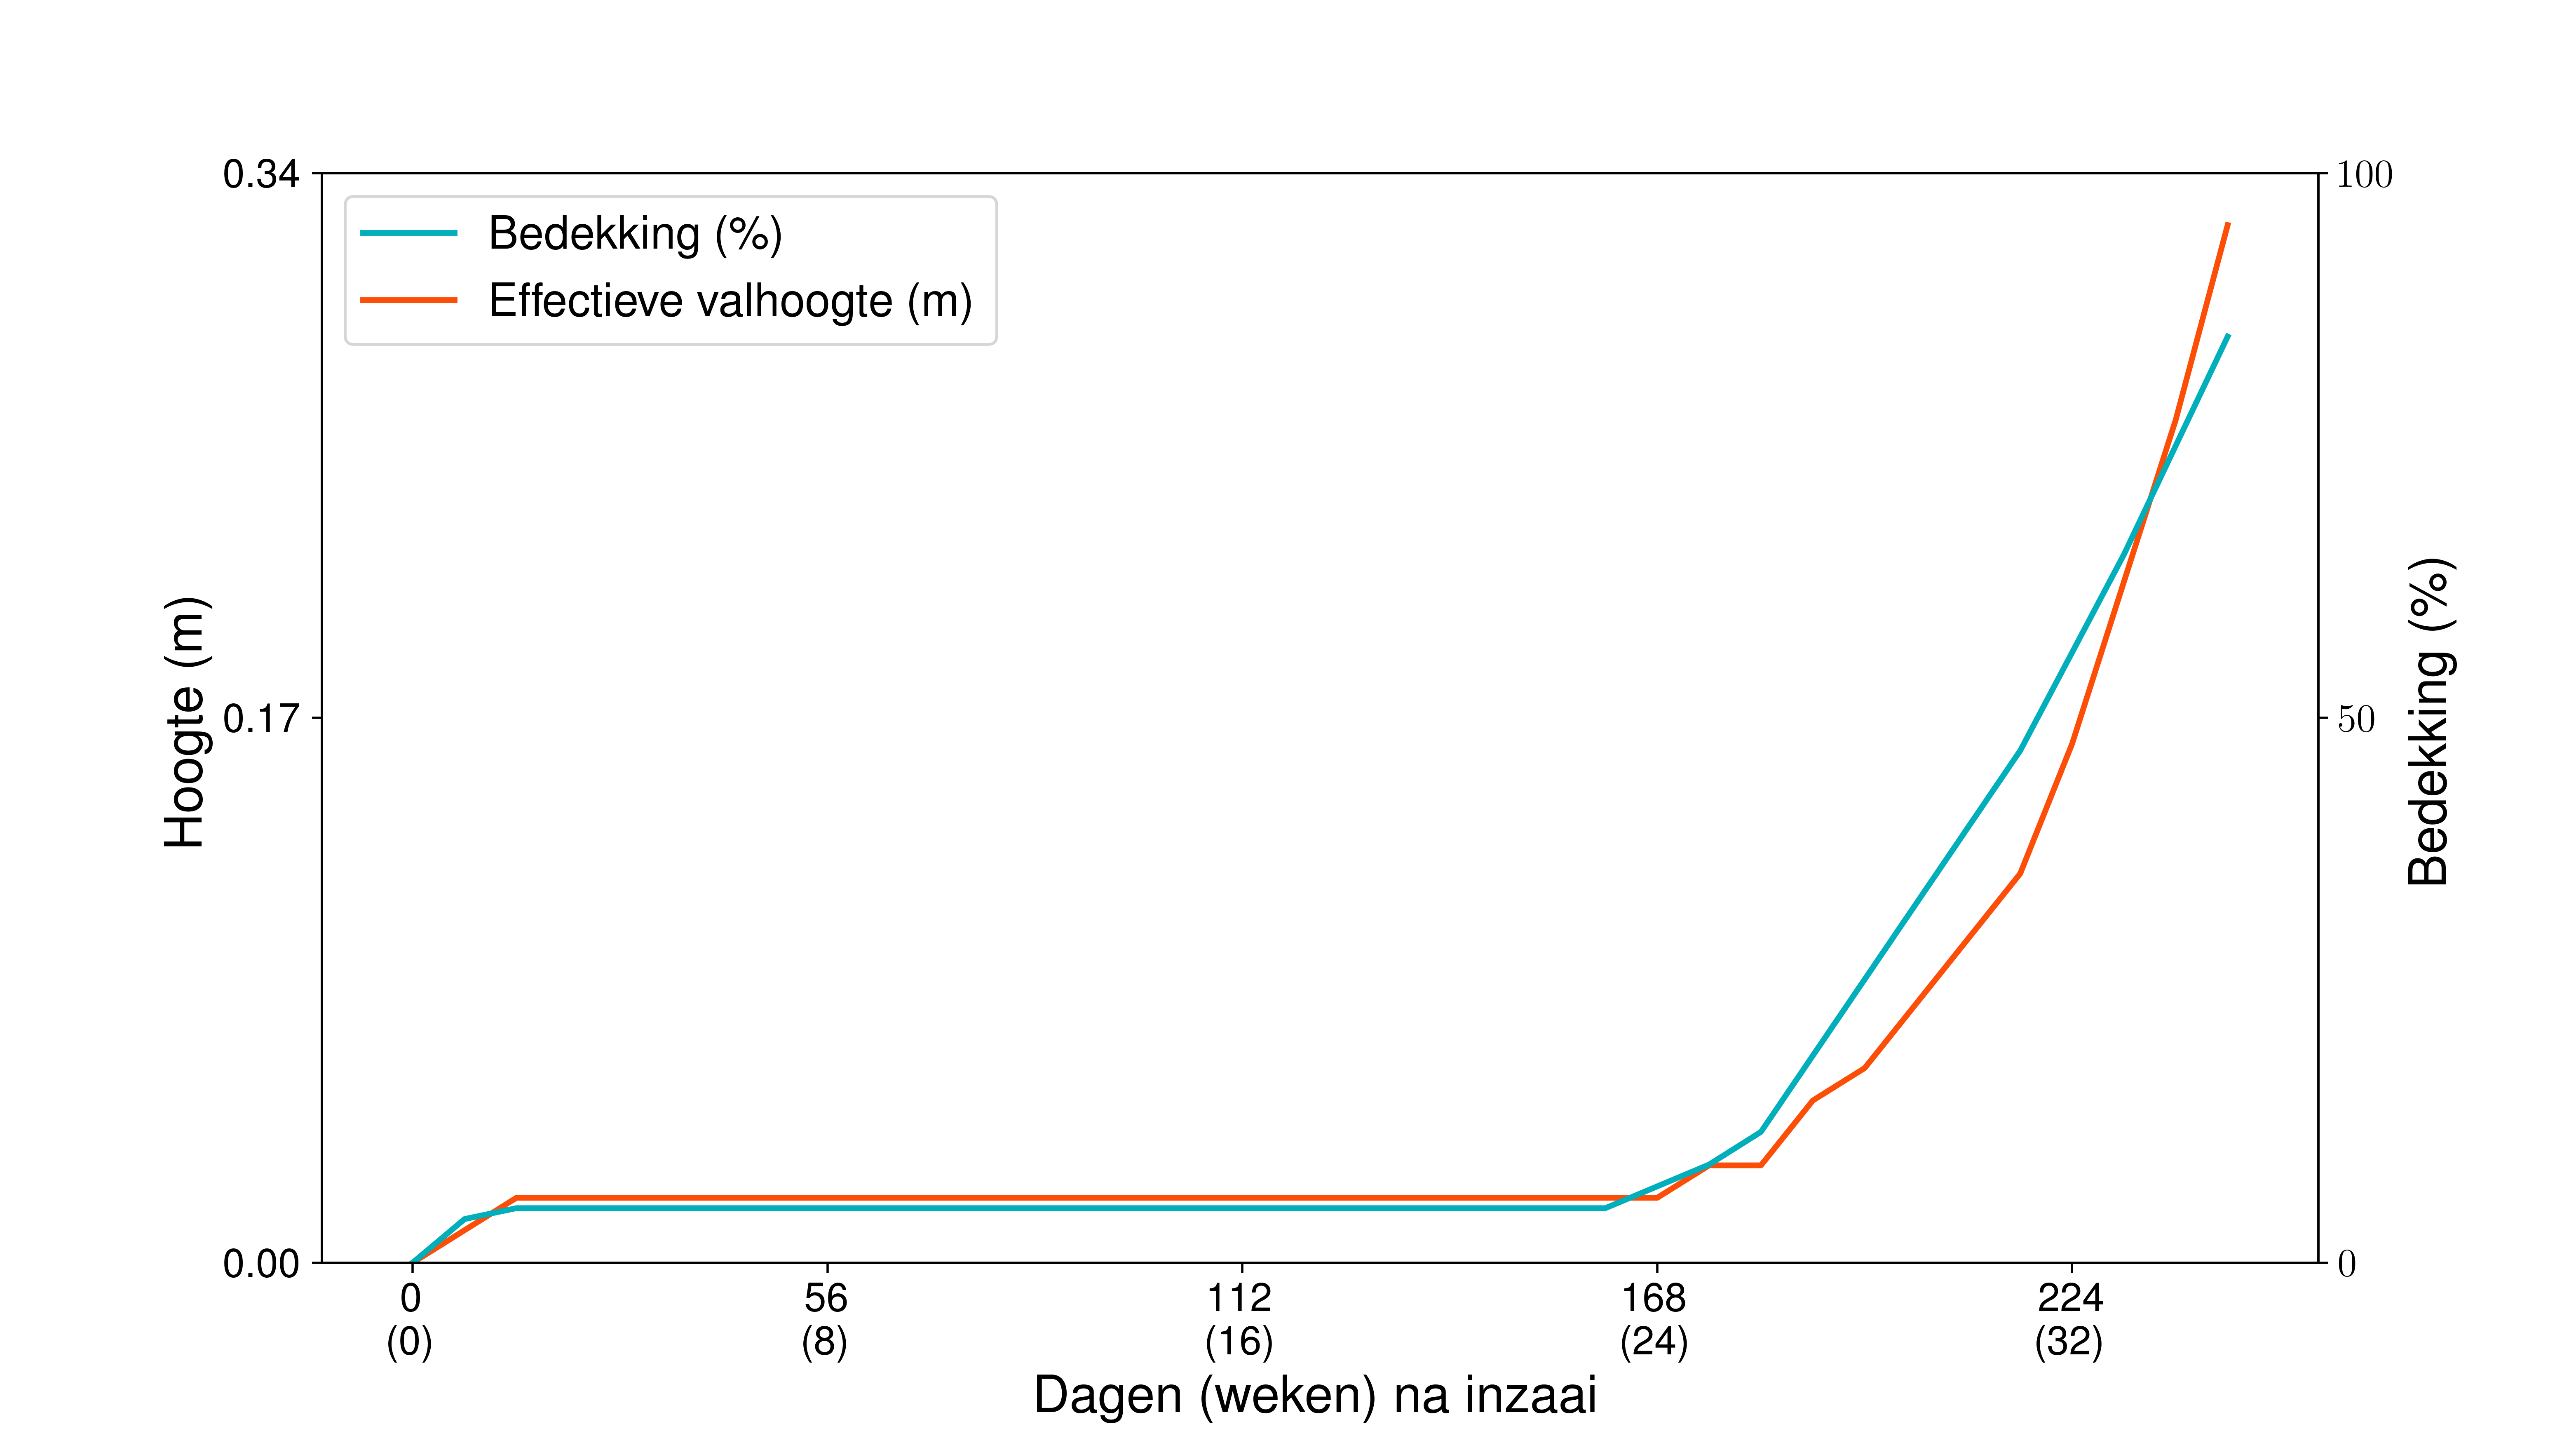
\includegraphics[width=12.5cm]{temp/2008.png} \end{figure} \end{center} 
  \textbf{Referenties:} Verbist2004;Gabriels2003;KMI2003;ILVO2019;Gobin2013 \vspace{0.10cm} \\ 
  \textbf{Opmerkingen?} overerving wintergerst: (Als er nateelt(jaar i-1) == brouwersgerst en-of voorteelt (jaar i)== brouwersgerst ) en hoofdteelt (jaar i) == brouwersgerst \vspace{0.10cm} \\ 
 \newpage 
 \subsection{Hoofdteelt (subgroep\_id 1010)} 
  \textbf{Zaaidatum (dd/mm)}: 15/03  \vspace{0.10cm} \\ 
  \textbf{Oogstdatum (dd/mm)}: 15/08  \vspace{0.10cm} \\ 
  \textbf{Oogstresten} \vspace{0.05cm} \\ 
  \tab Initi\"{e}le hoeveelheid (kg ha$^{-1}$): 3600.00 \vspace{0.05cm} \\ 
  \tab Afbraakcoefficient (-): 0.01 \vspace{0.05cm} \\ 
  \tab Bodembedekking (m$^2$ kg$^{-1}$): 1.20 \vspace{0.05cm} \\ 
  \tab Initieel percentage bedekking (\%): 100 \vspace{0.05cm} \\ 
  \tab Halfwaarde tijd (dagen): 30 \vspace{0.05cm} \\ 
  \textbf{Initi\"{e}le bodemruwheid (mm)}: 10.20 \vspace{0.05cm} \\ 
  \textbf{Gewasgroeicurve subgroep\_id 1010:} 
 \begin{center} \begin{figure}[H] 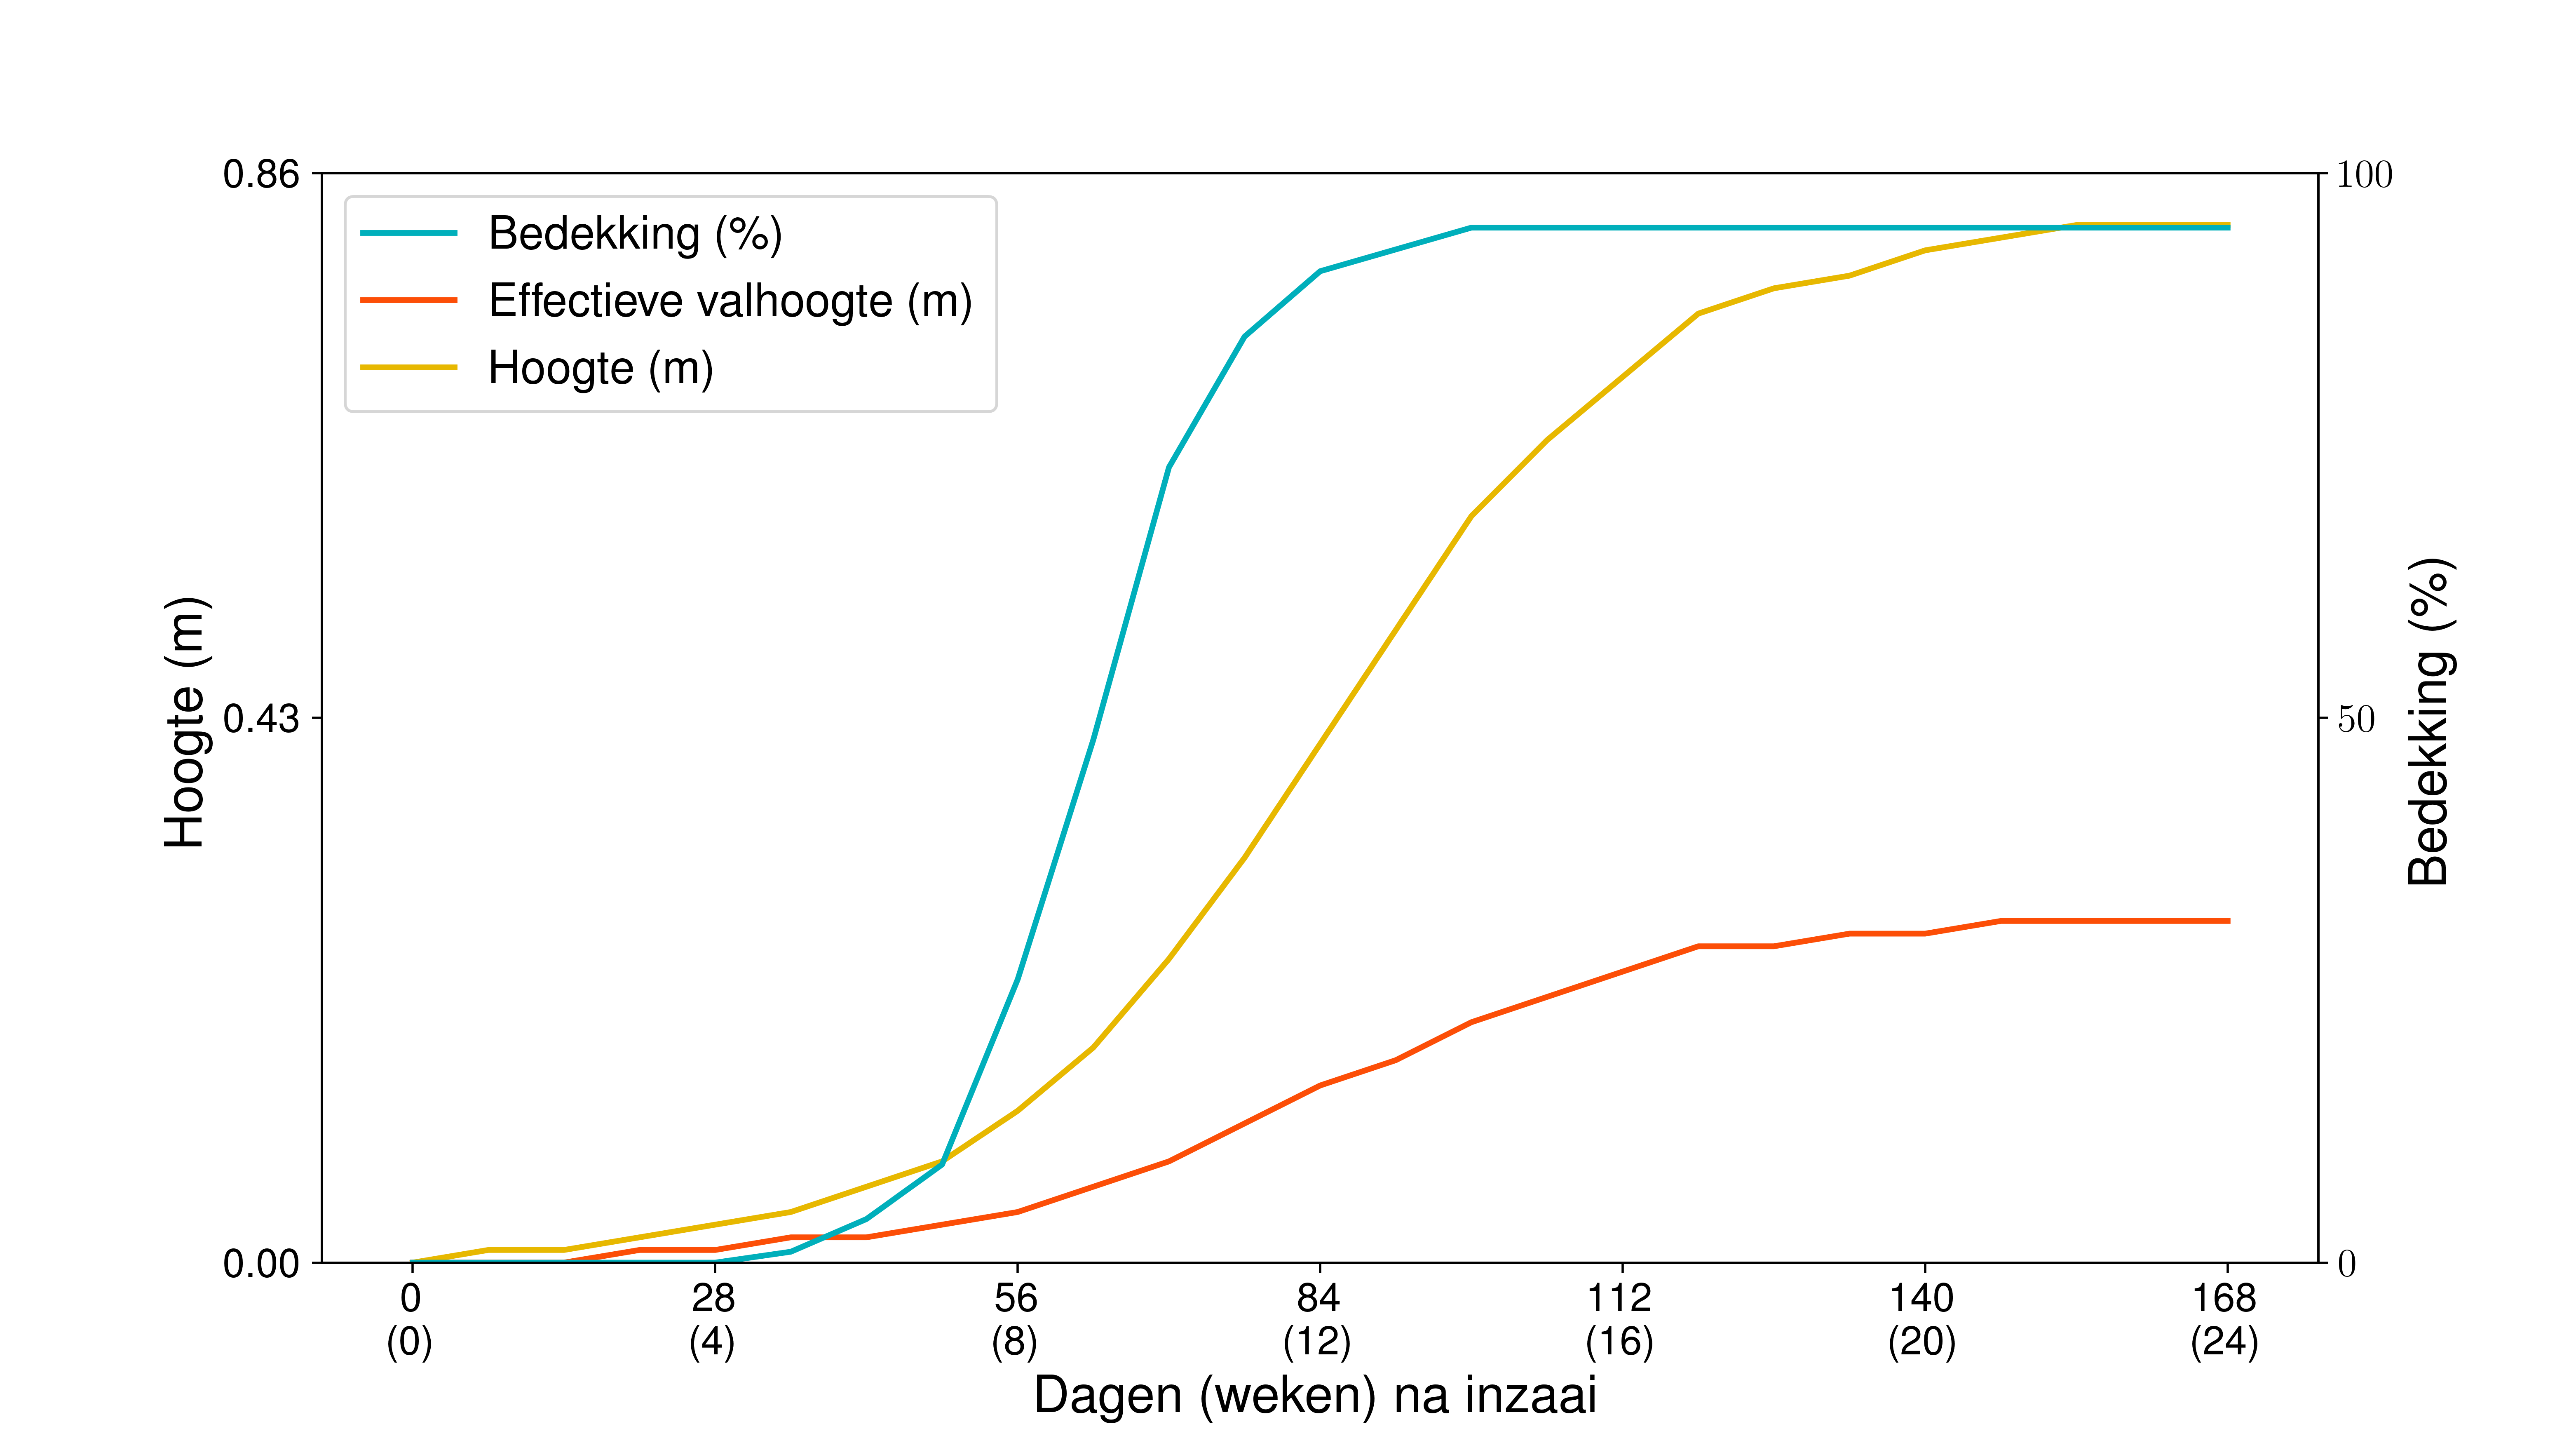
\includegraphics[width=12.5cm]{temp/1010.png} \end{figure} \end{center} 
  \textbf{Referenties:} Verbist2004;Gabriels2003;KMI2003;ILVO2019;Gobin2013 \vspace{0.10cm} \\ 
  \textbf{Opmerkingen?} overerving zomergerst: andere gevallen \vspace{0.10cm} \\ 
 \newpage 
 \section{Zomerhaver (groep\_id 13)} 
 \textbf{Van toepassing op gewasnamen (en codes):} Zomerhaver (342) 
 \begin{multicols}{3} \begin{itemize} \item[$\square$] Meerjarig \item[$\square$] Groenbedekker \item[$\square$] Groente \end{itemize} \end{multicols} 
  \textbf{Zaaidatum (dd/mm)}: 28/02  \vspace{0.10cm} \\ 
  \textbf{Oogstdatum (dd/mm)}: 15/08  \vspace{0.10cm} \\ 
  \textbf{Oogstresten} \vspace{0.05cm} \\ 
  \tab Initi\"{e}le hoeveelheid (kg ha$^{-1}$): 376.00 \vspace{0.05cm} \\ 
  \tab Afbraakcoefficient (-): 0.02 \vspace{0.05cm} \\ 
  \tab Bodembedekking (m$^2$ kg$^{-1}$): 2.55 \vspace{0.05cm} \\ 
  \tab Initieel percentage bedekking (\%): 9 \vspace{0.05cm} \\ 
  \tab Halfwaarde tijd (dagen): 15 \vspace{0.05cm} \\ 
  \textbf{Initi\"{e}le bodemruwheid (mm)}: 7.60 \vspace{0.05cm} \\ 
  \textbf{Gewasgroeicurve subgroep\_id 1013:} 
 \begin{center} \begin{figure}[H] 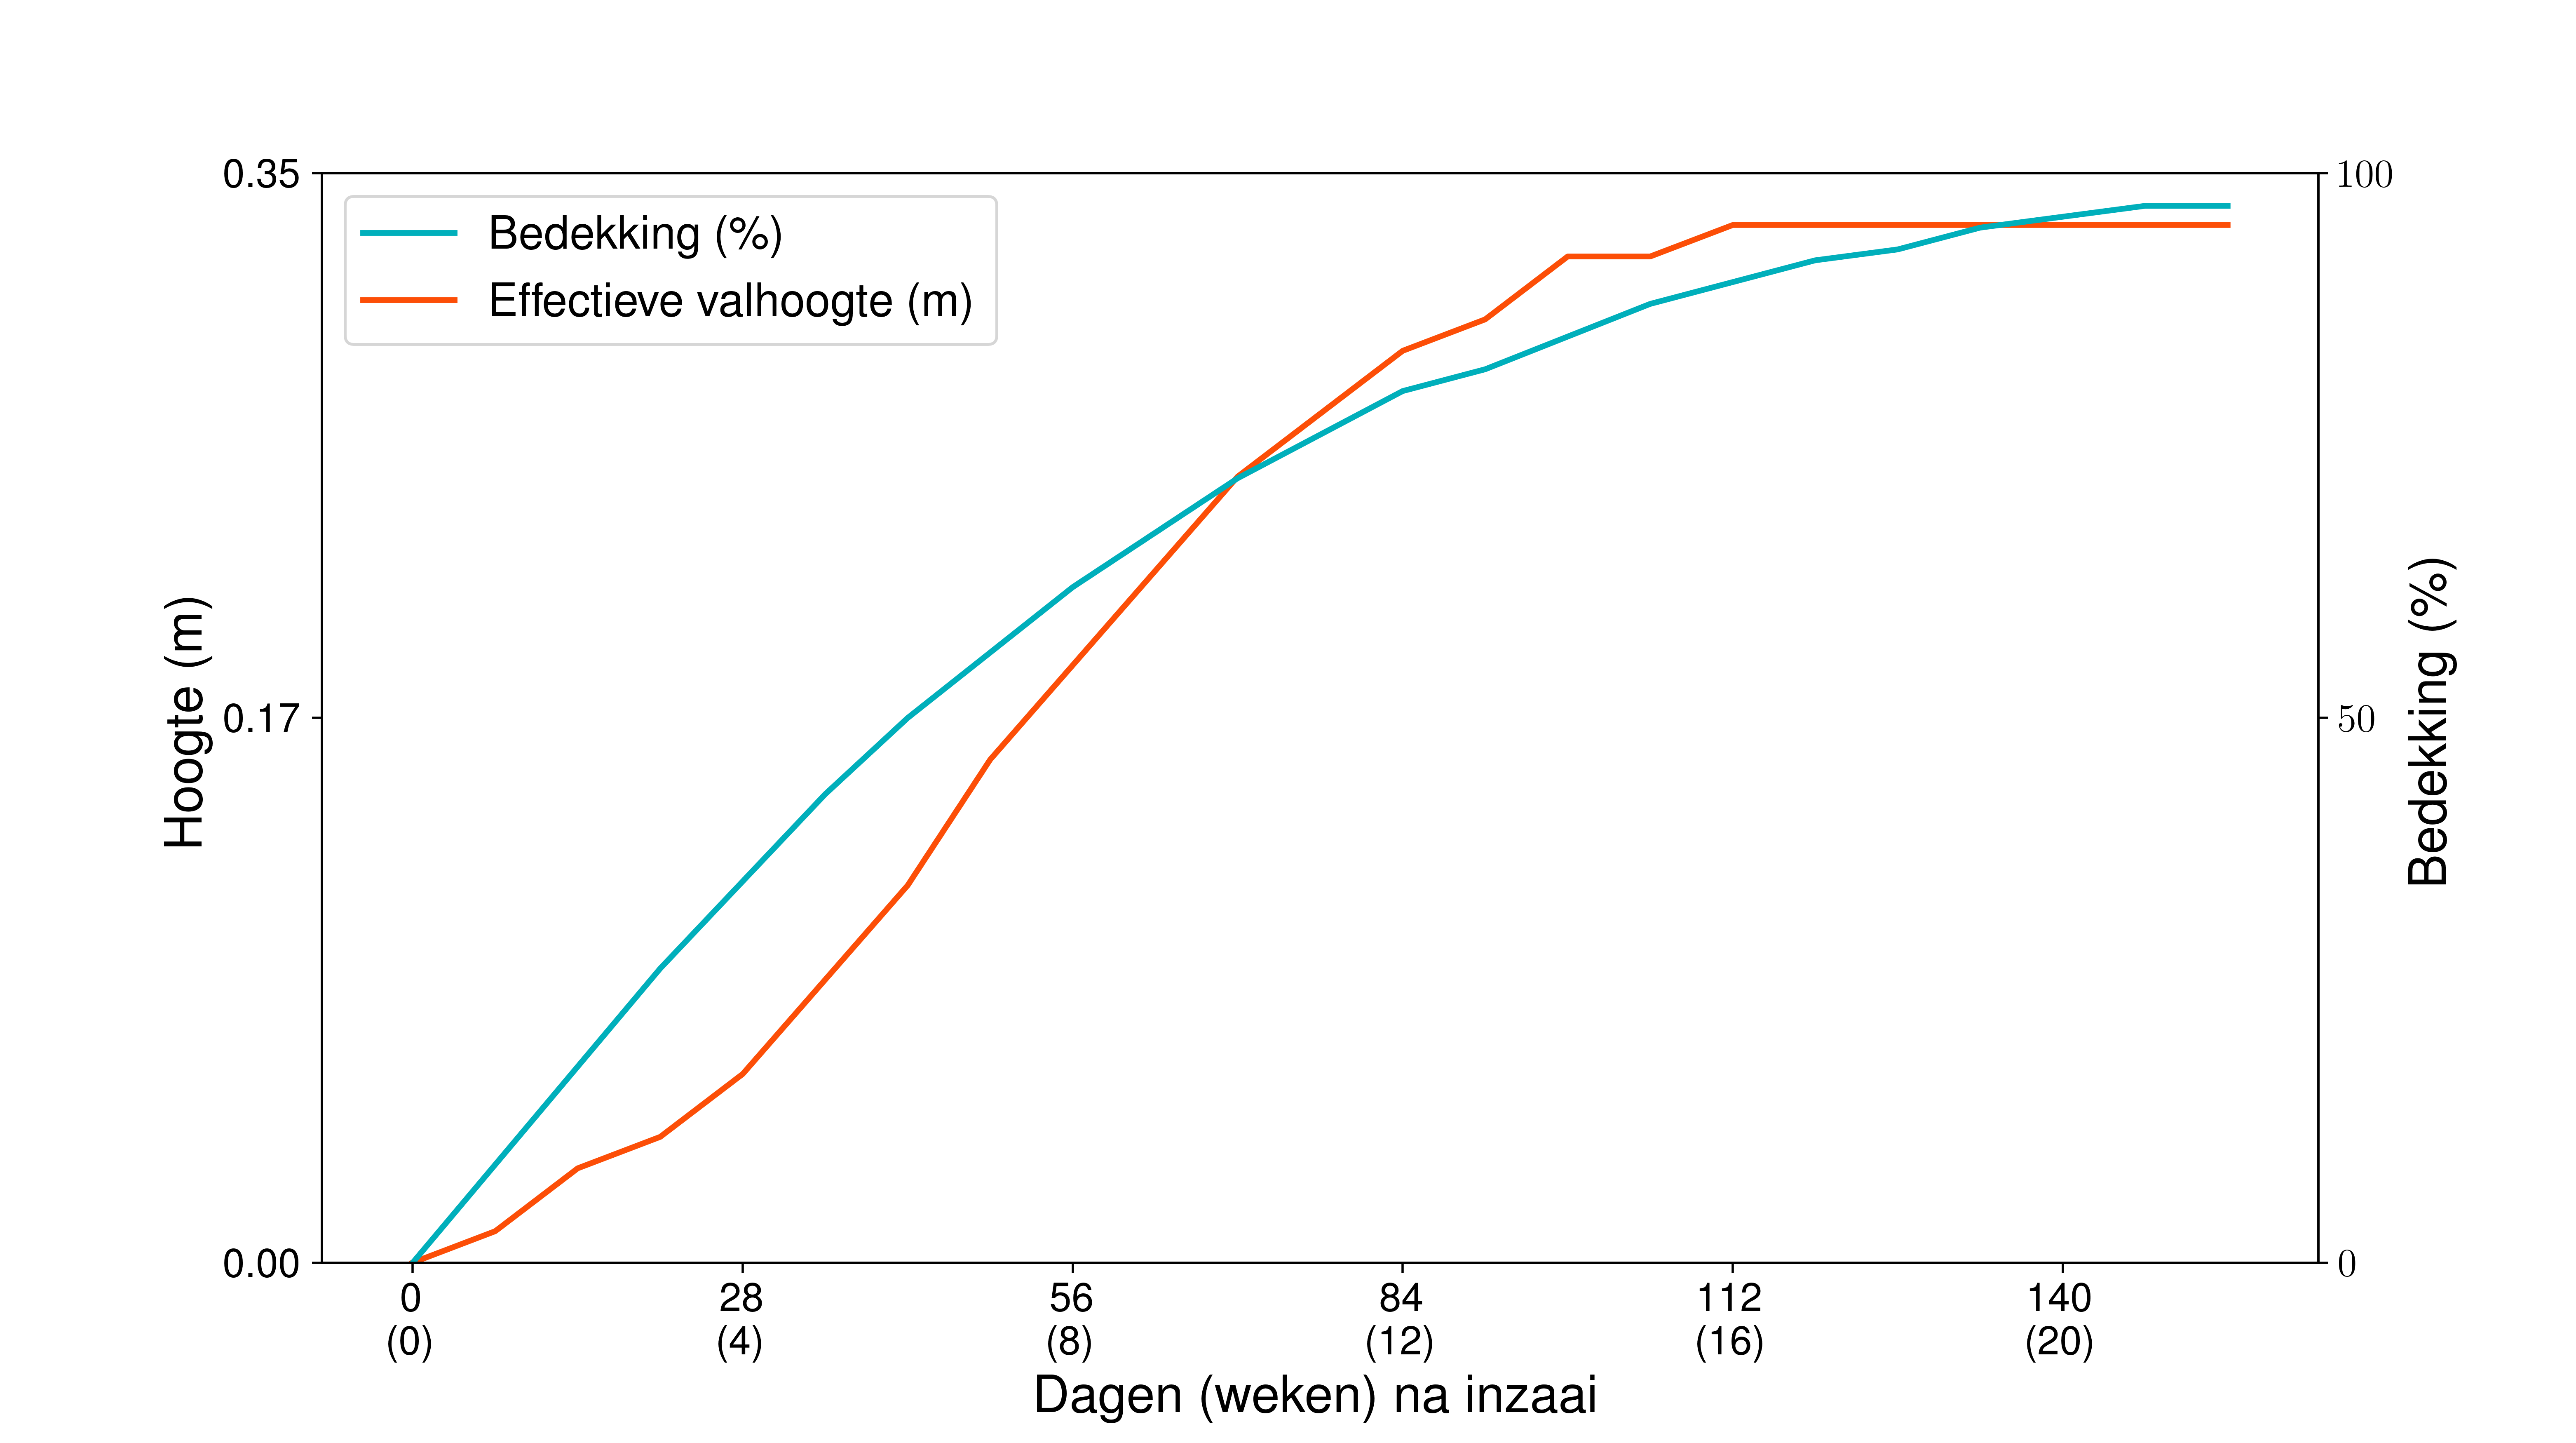
\includegraphics[width=12.5cm]{temp/1013.png} \end{figure} \end{center} 
  \textbf{Referenties:} ILVO2019;RUSLE \vspace{0.10cm} \\ 
  \textbf{Opmerkingen?} geen \vspace{0.10cm} \\ 
 \newpage 
 \section{Vezelvlas (vezelproductie) (groep\_id 14)} 
 \textbf{Van toepassing op gewasnamen (en codes):} Vezelvlas (bestemd voor vezelproductie) (921) 
 \begin{multicols}{3} \begin{itemize} \item[$\square$] Meerjarig \item[$\square$] Groenbedekker \item[$\square$] Groente \end{itemize} \end{multicols} 
  \textbf{Zaaidatum (dd/mm)}: 15/03  \vspace{0.10cm} \\ 
  \textbf{Oogstdatum (dd/mm)}: 01/07  \vspace{0.10cm} \\ 
  \textbf{Oogstresten} \vspace{0.05cm} \\ 
  \tab Initi\"{e}le hoeveelheid (kg ha$^{-1}$): 0.00 \vspace{0.05cm} \\ 
  \tab Afbraakcoefficient (-): 0.00 \vspace{0.05cm} \\ 
  \tab Bodembedekking (m$^2$ kg$^{-1}$): 0.00 \vspace{0.05cm} \\ 
  \tab Initieel percentage bedekking (\%): 0 \vspace{0.05cm} \\ 
  \tab Halfwaarde tijd (dagen): 0 \vspace{0.05cm} \\ 
  \textbf{Initi\"{e}le bodemruwheid (mm)}: 7.60 \vspace{0.05cm} \\ 
  \textbf{Gewasgroeicurve subgroep\_id 1014:} 
 \begin{center} \begin{figure}[H] 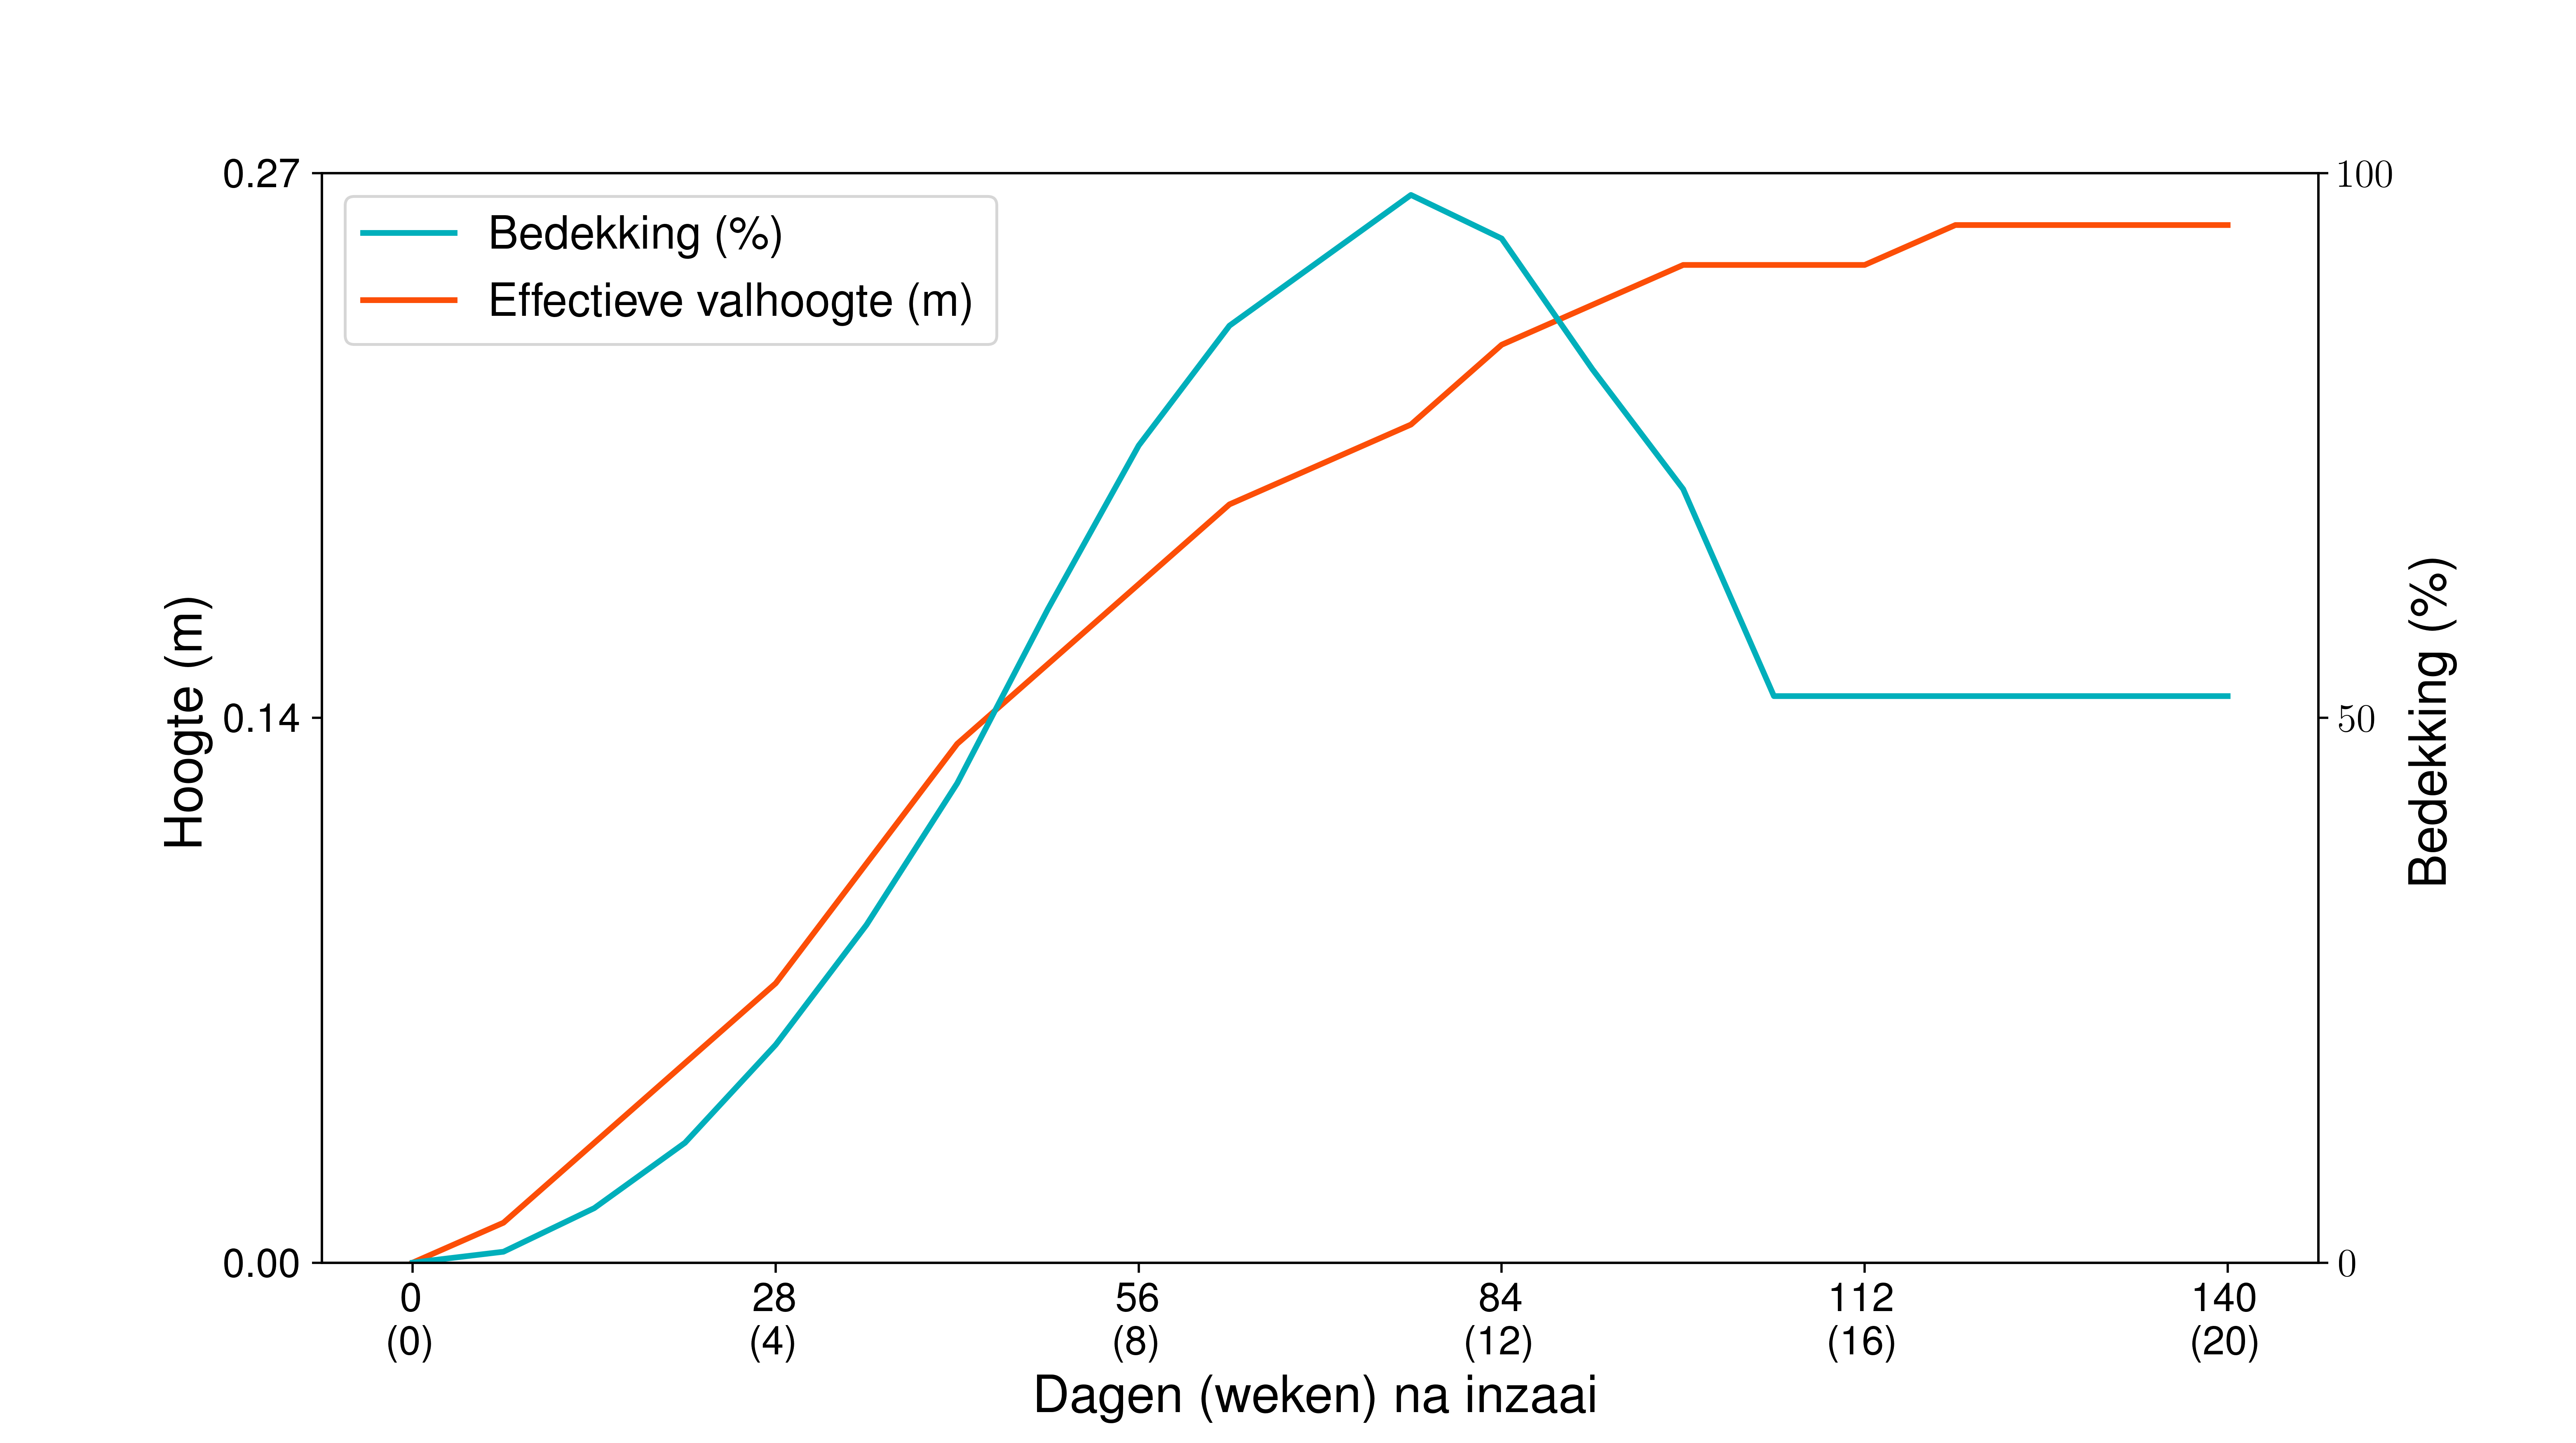
\includegraphics[width=12.5cm]{temp/1014.png} \end{figure} \end{center} 
  \textbf{Referenties:} Bodemkundige Dienst van Belgie \vspace{0.10cm} \\ 
  \textbf{Opmerkingen?} geen \vspace{0.10cm} \\ 
 \newpage 
 \section{Hop (groep\_id 15)} 
 \textbf{Van toepassing op gewasnamen (en codes):} Hop (9822) 
 \begin{multicols}{3} \begin{itemize} \item[$\square$] Meerjarig \item[$\square$] Groenbedekker \item[$\square$] Groente \end{itemize} \end{multicols} 
  \textbf{Zaaidatum (dd/mm)}: 15/03  \vspace{0.10cm} \\ 
  \textbf{Oogstdatum (dd/mm)}: 01/09  \vspace{0.10cm} \\ 
  \textbf{Oogstresten} \vspace{0.05cm} \\ 
  \tab Initi\"{e}le hoeveelheid (kg ha$^{-1}$): 0.00 \vspace{0.05cm} \\ 
  \tab Afbraakcoefficient (-): 0.00 \vspace{0.05cm} \\ 
  \tab Bodembedekking (m$^2$ kg$^{-1}$): 0.00 \vspace{0.05cm} \\ 
  \tab Initieel percentage bedekking (\%): 0 \vspace{0.05cm} \\ 
  \tab Halfwaarde tijd (dagen): 0 \vspace{0.05cm} \\ 
  \textbf{Initi\"{e}le bodemruwheid (mm)}: 10.20 \vspace{0.05cm} \\ 
  \textbf{Gewasgroeicurve subgroep\_id 1015:} 
 \begin{center} \begin{figure}[H] 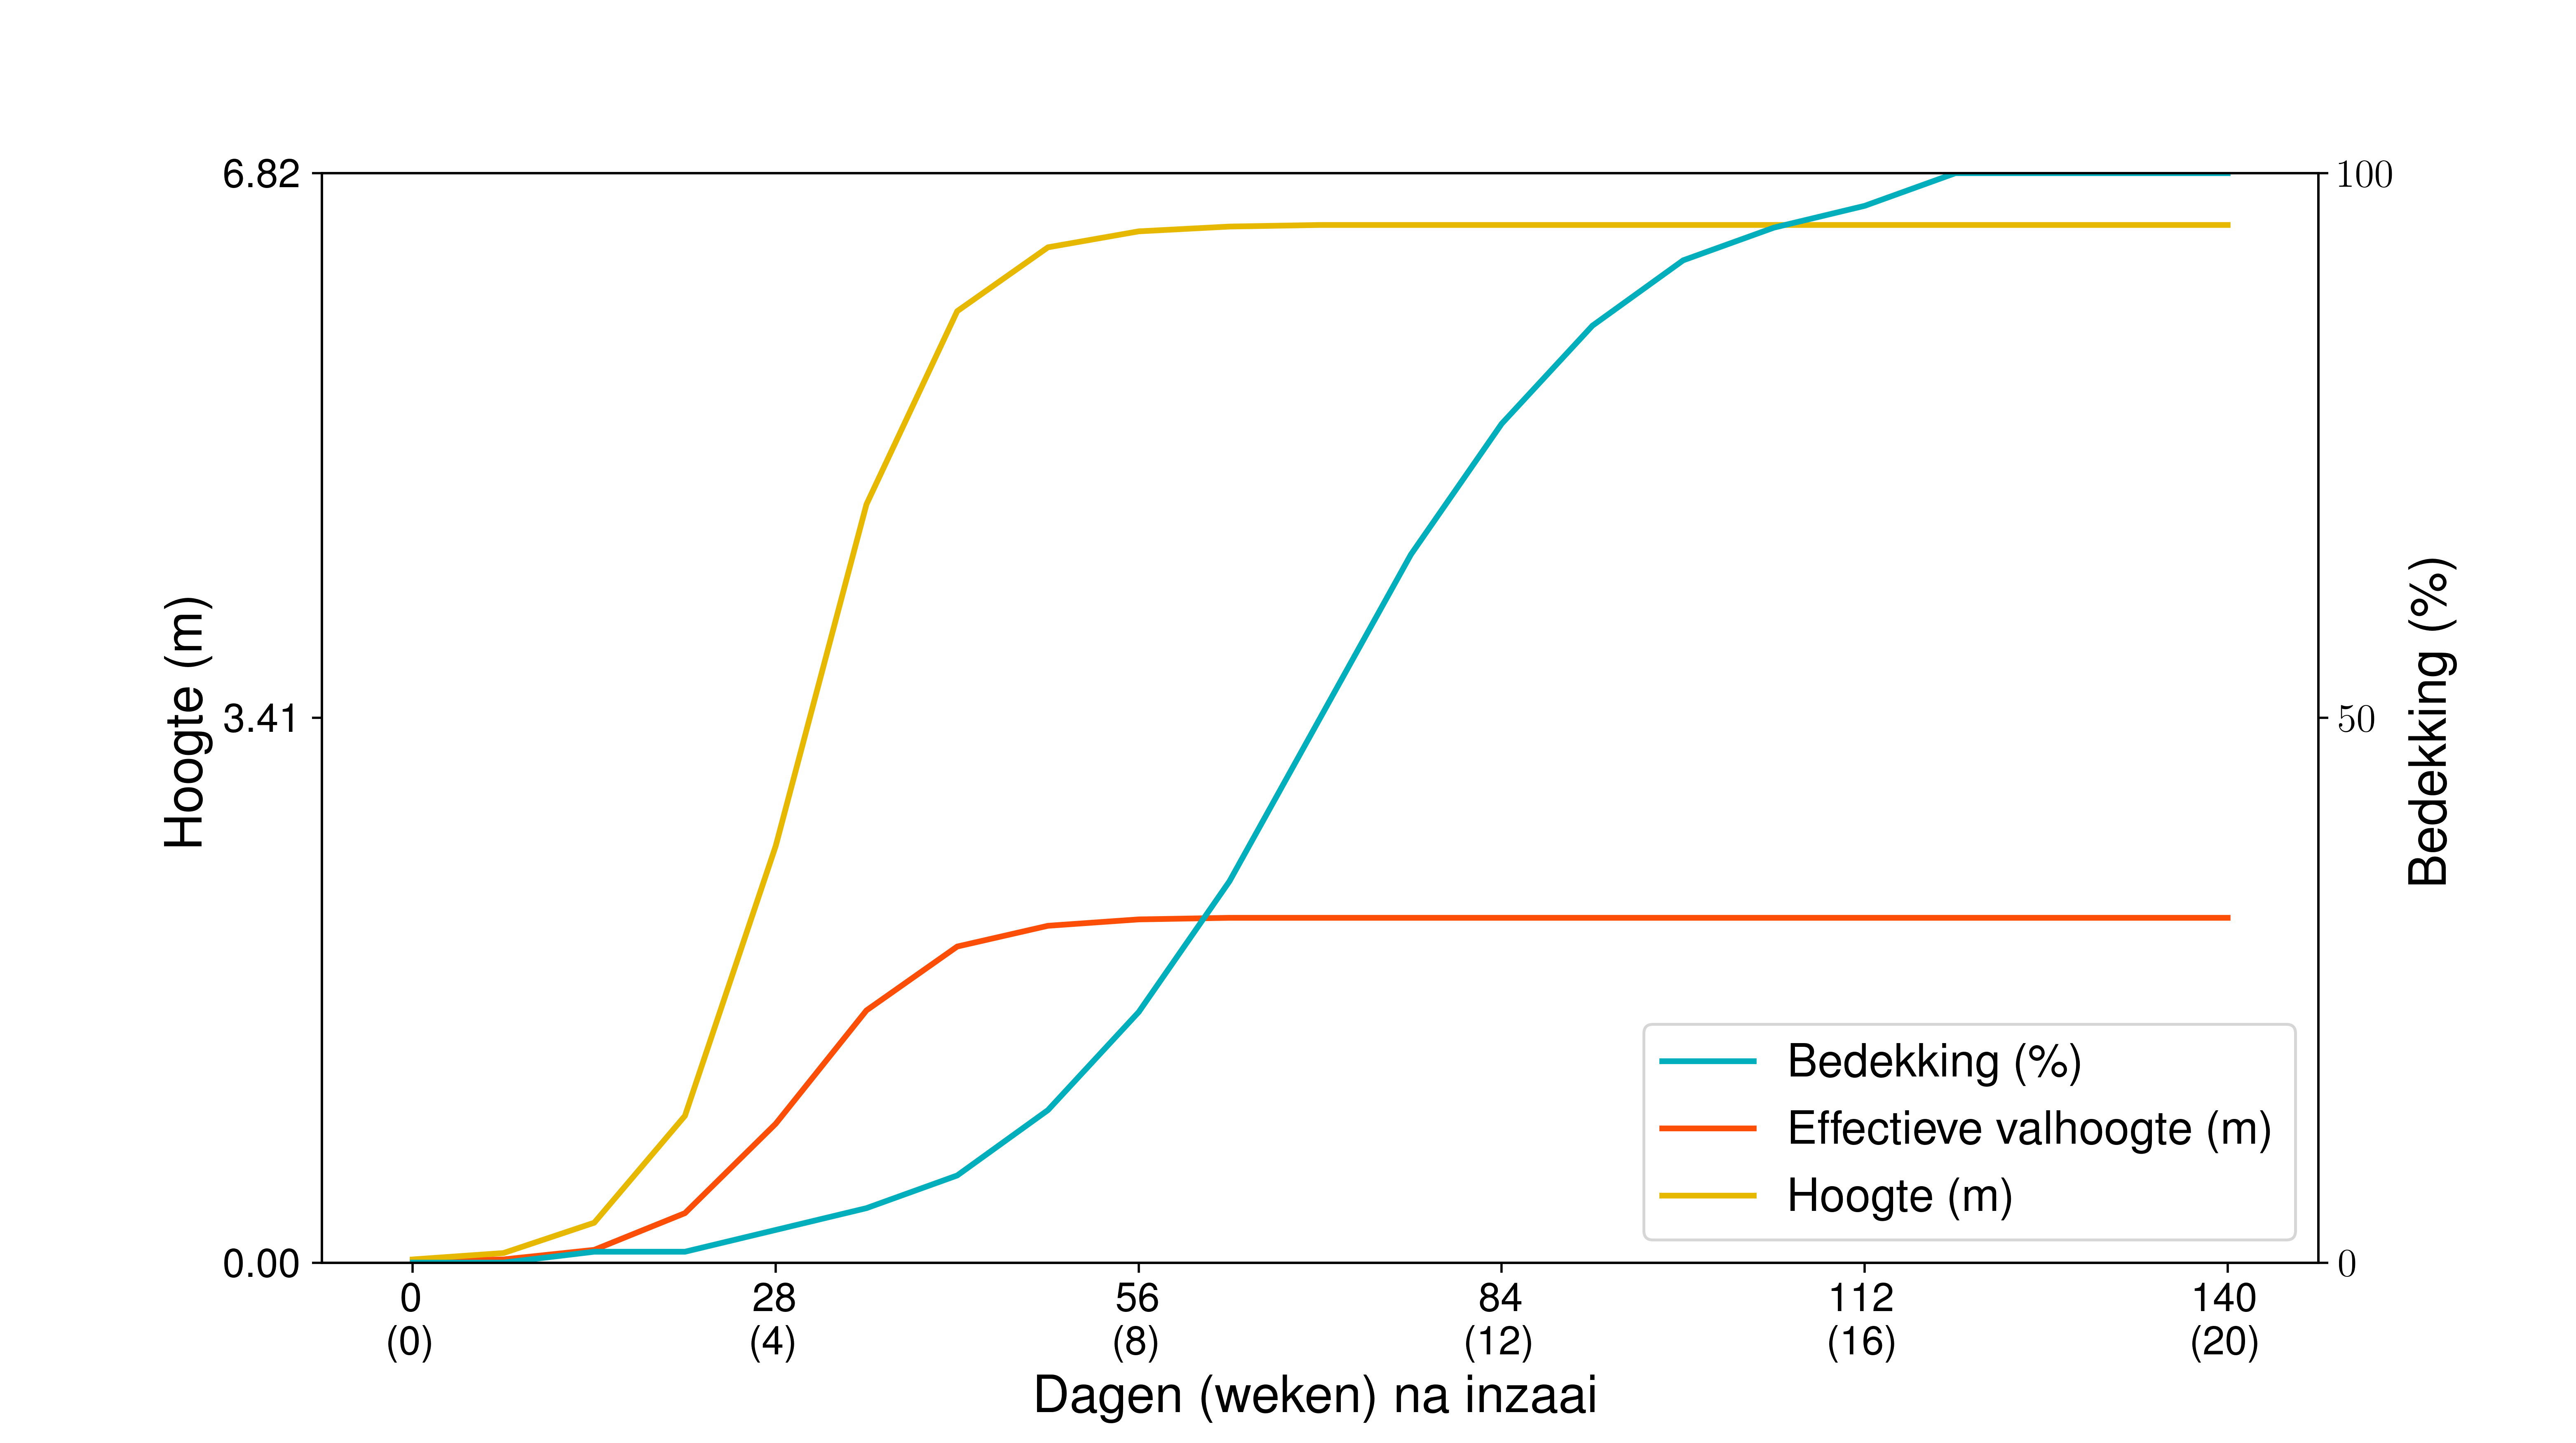
\includegraphics[width=12.5cm]{temp/1015.png} \end{figure} \end{center} 
  \textbf{Referenties:} ILVO2019 \vspace{0.10cm} \\ 
  \textbf{Opmerkingen?} geen \vspace{0.10cm} \\ 
 \newpage 
 \section{Gras (groep\_id 16)} 
 \textbf{Van toepassing op gewasnamen (en codes):} Grasland (60) , Grasklaver (700) 
 \begin{multicols}{3} \begin{itemize} \item[$\boxtimes$] Meerjarig \item[$\boxtimes$] Groenbedekker \item[$\square$] Groente \end{itemize} \end{multicols} 
 \subsection{Hoofdteelt (subgroep\_id 1016)} 
  \textbf{Zaaidatum (dd/mm)}: 01/04  \vspace{0.10cm} \\ 
  \textbf{Oogstdatum (dd/mm)}: /9  \vspace{0.10cm} \\ 
  \textbf{Oogstresten} \vspace{0.05cm} \\ 
  \tab Initi\"{e}le hoeveelheid (kg ha$^{-1}$): 2500.00 \vspace{0.05cm} \\ 
  \tab Afbraakcoefficient (-): 0.01 \vspace{0.05cm} \\ 
  \tab Bodembedekking (m$^2$ kg$^{-1}$): 11.98 \vspace{0.05cm} \\ 
  \tab Initieel percentage bedekking (\%): 95 \vspace{0.05cm} \\ 
  \tab Halfwaarde tijd (dagen): 30 \vspace{0.05cm} \\ 
  \textbf{Initi\"{e}le bodemruwheid (mm)}: 7.60 \vspace{0.05cm} \\ 
  \textbf{Gewasgroeicurve subgroep\_id 1016:} 
 \begin{center} \begin{figure}[H] 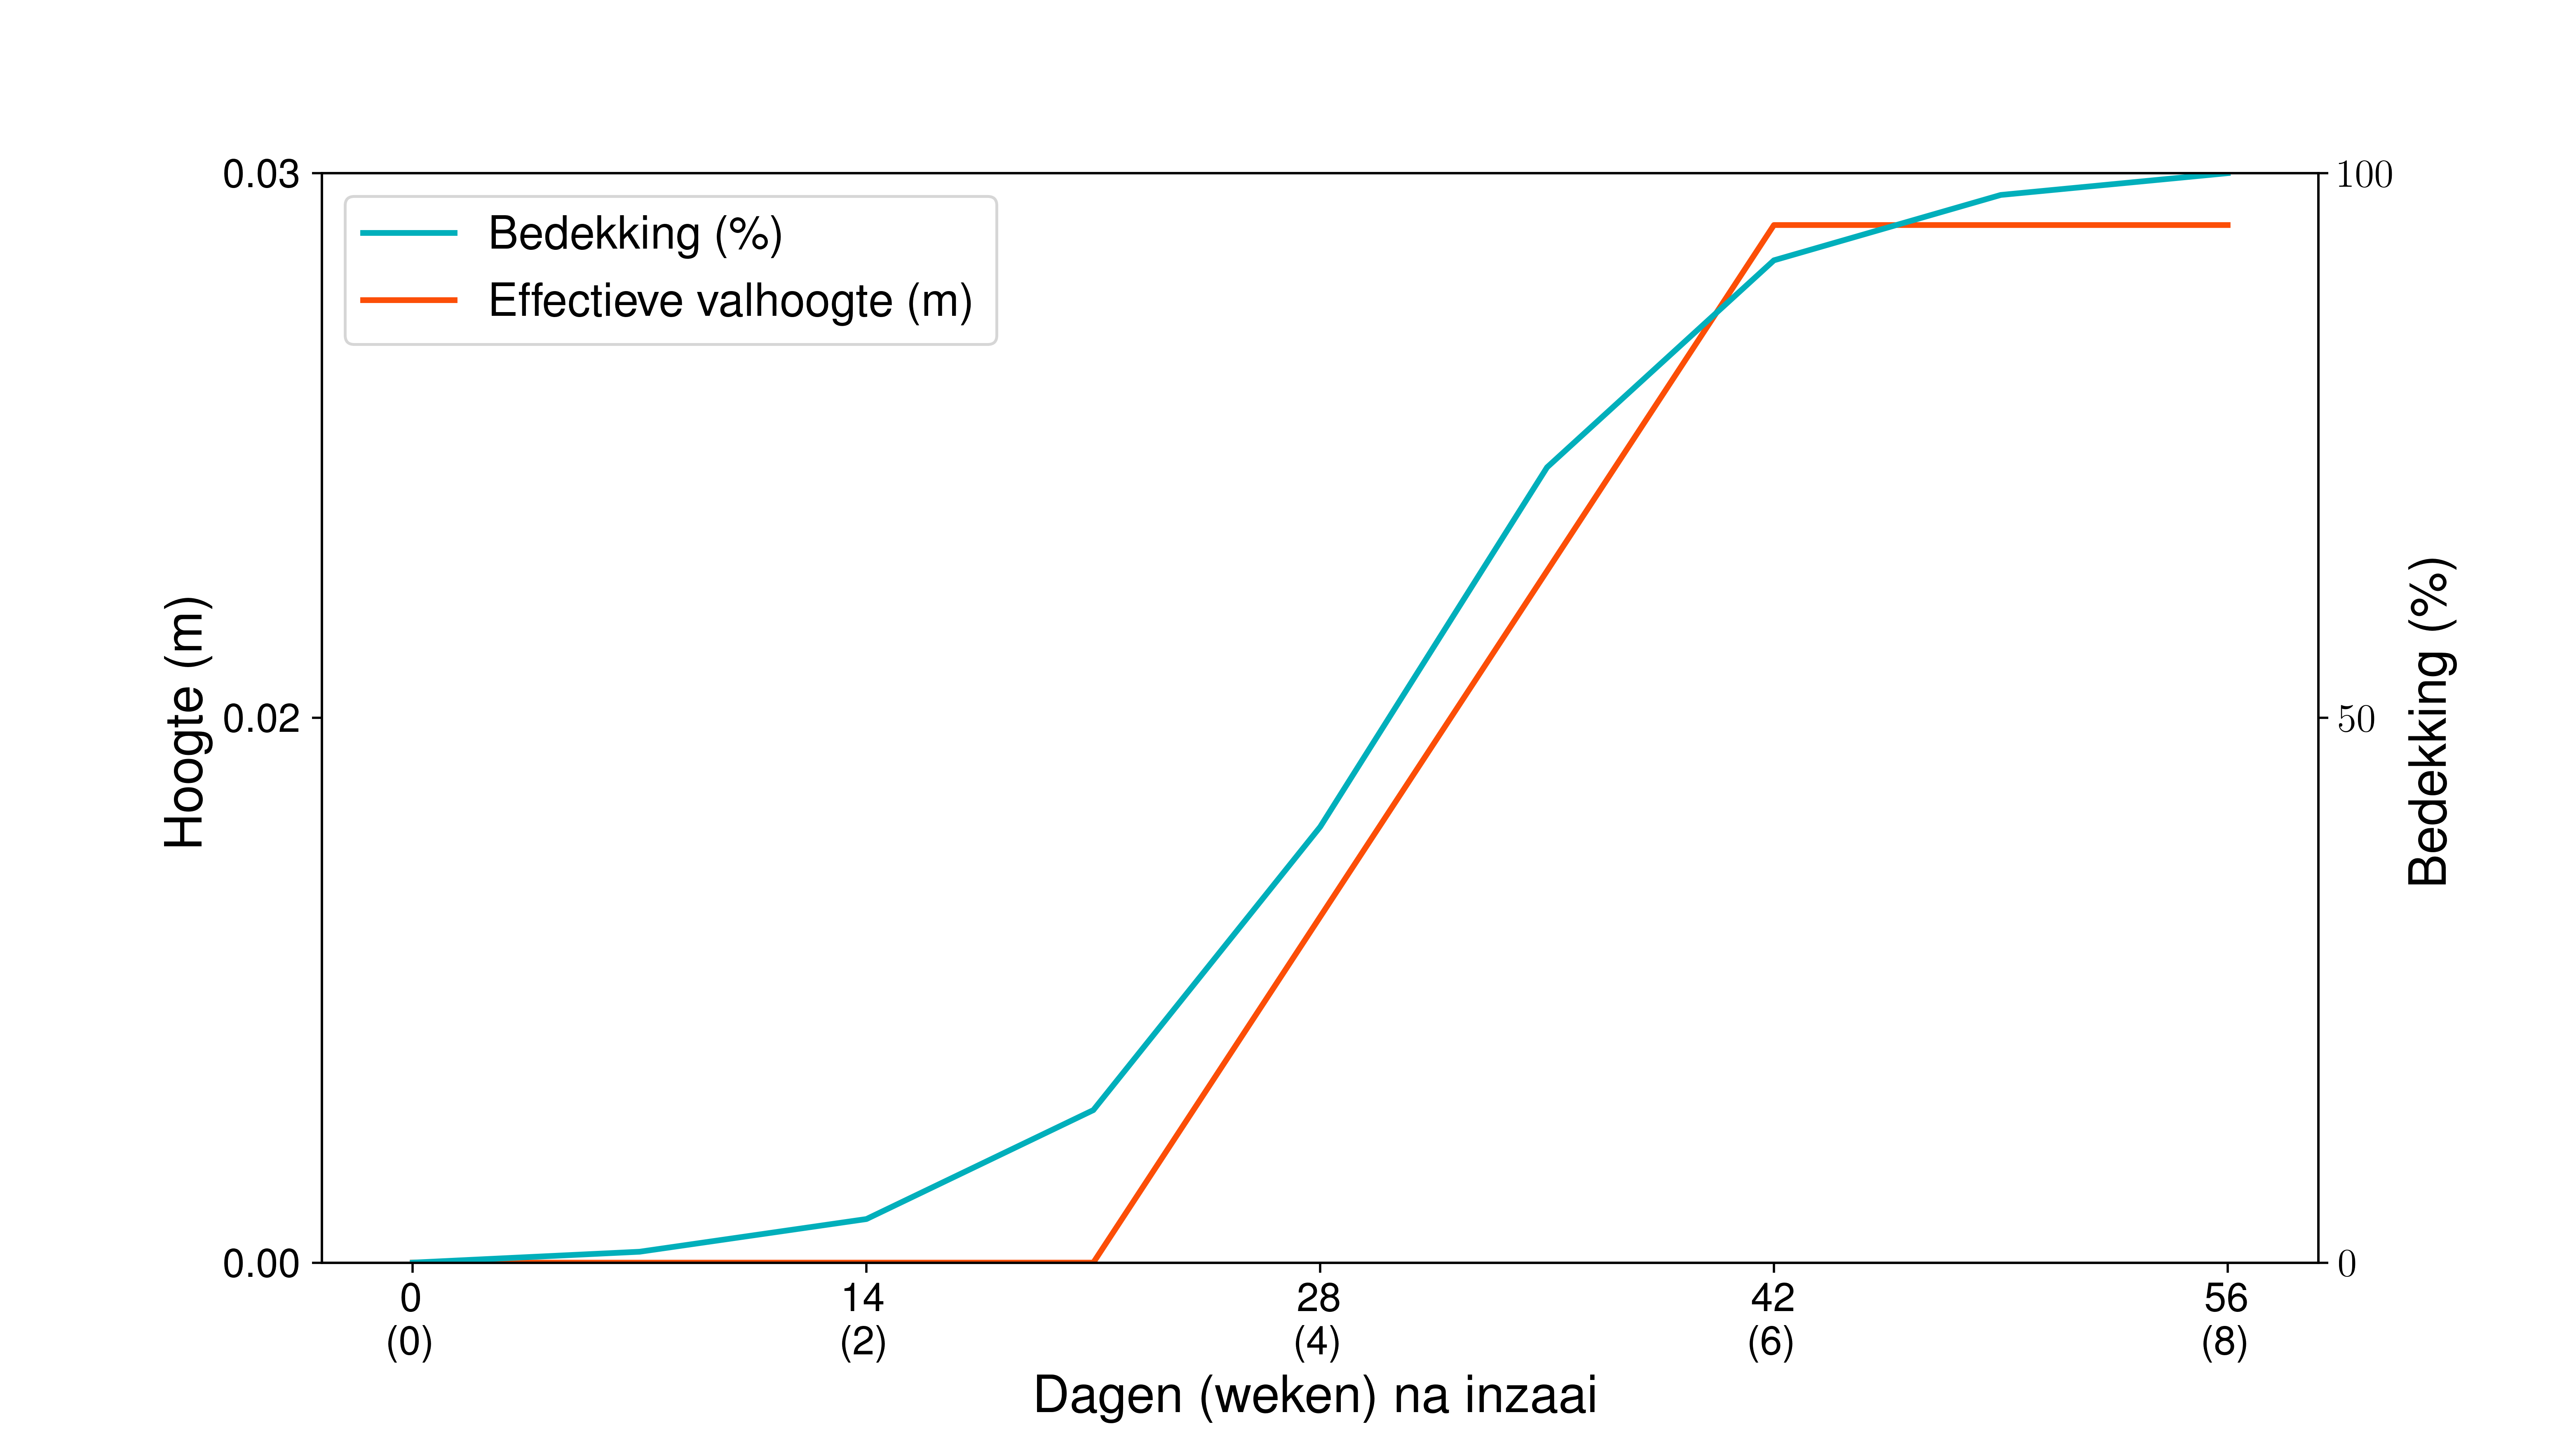
\includegraphics[width=12.5cm]{temp/1016.png} \end{figure} \end{center} 
  \textbf{Referenties:} Gabriels2003;KMI2003;RUSLE;ILVO2019 \vspace{0.10cm} \\ 
  \textbf{Opmerkingen?} geen \vspace{0.10cm} \\ 
 \newpage 
 \subsection{Nateelt (inzaaidatum=[0901,0930]) (subgroep\_id 2016)} 
  \textbf{Zaaidatum (dd/mm)}: 01/09  \vspace{0.10cm} \\ 
  \textbf{Oogstdatum (dd/mm)}: /9  \vspace{0.10cm} \\ 
  \textbf{Oogstresten} \vspace{0.05cm} \\ 
  \tab Initi\"{e}le hoeveelheid (kg ha$^{-1}$): 2500.00 \vspace{0.05cm} \\ 
  \tab Afbraakcoefficient (-): 0.01 \vspace{0.05cm} \\ 
  \tab Bodembedekking (m$^2$ kg$^{-1}$): 11.98 \vspace{0.05cm} \\ 
  \tab Initieel percentage bedekking (\%): 95 \vspace{0.05cm} \\ 
  \tab Halfwaarde tijd (dagen): 30 \vspace{0.05cm} \\ 
  \textbf{Initi\"{e}le bodemruwheid (mm)}: 7.60 \vspace{0.05cm} \\ 
  \textbf{Gewasgroeicurve subgroep\_id 2016:} 
 \begin{center} \begin{figure}[H] 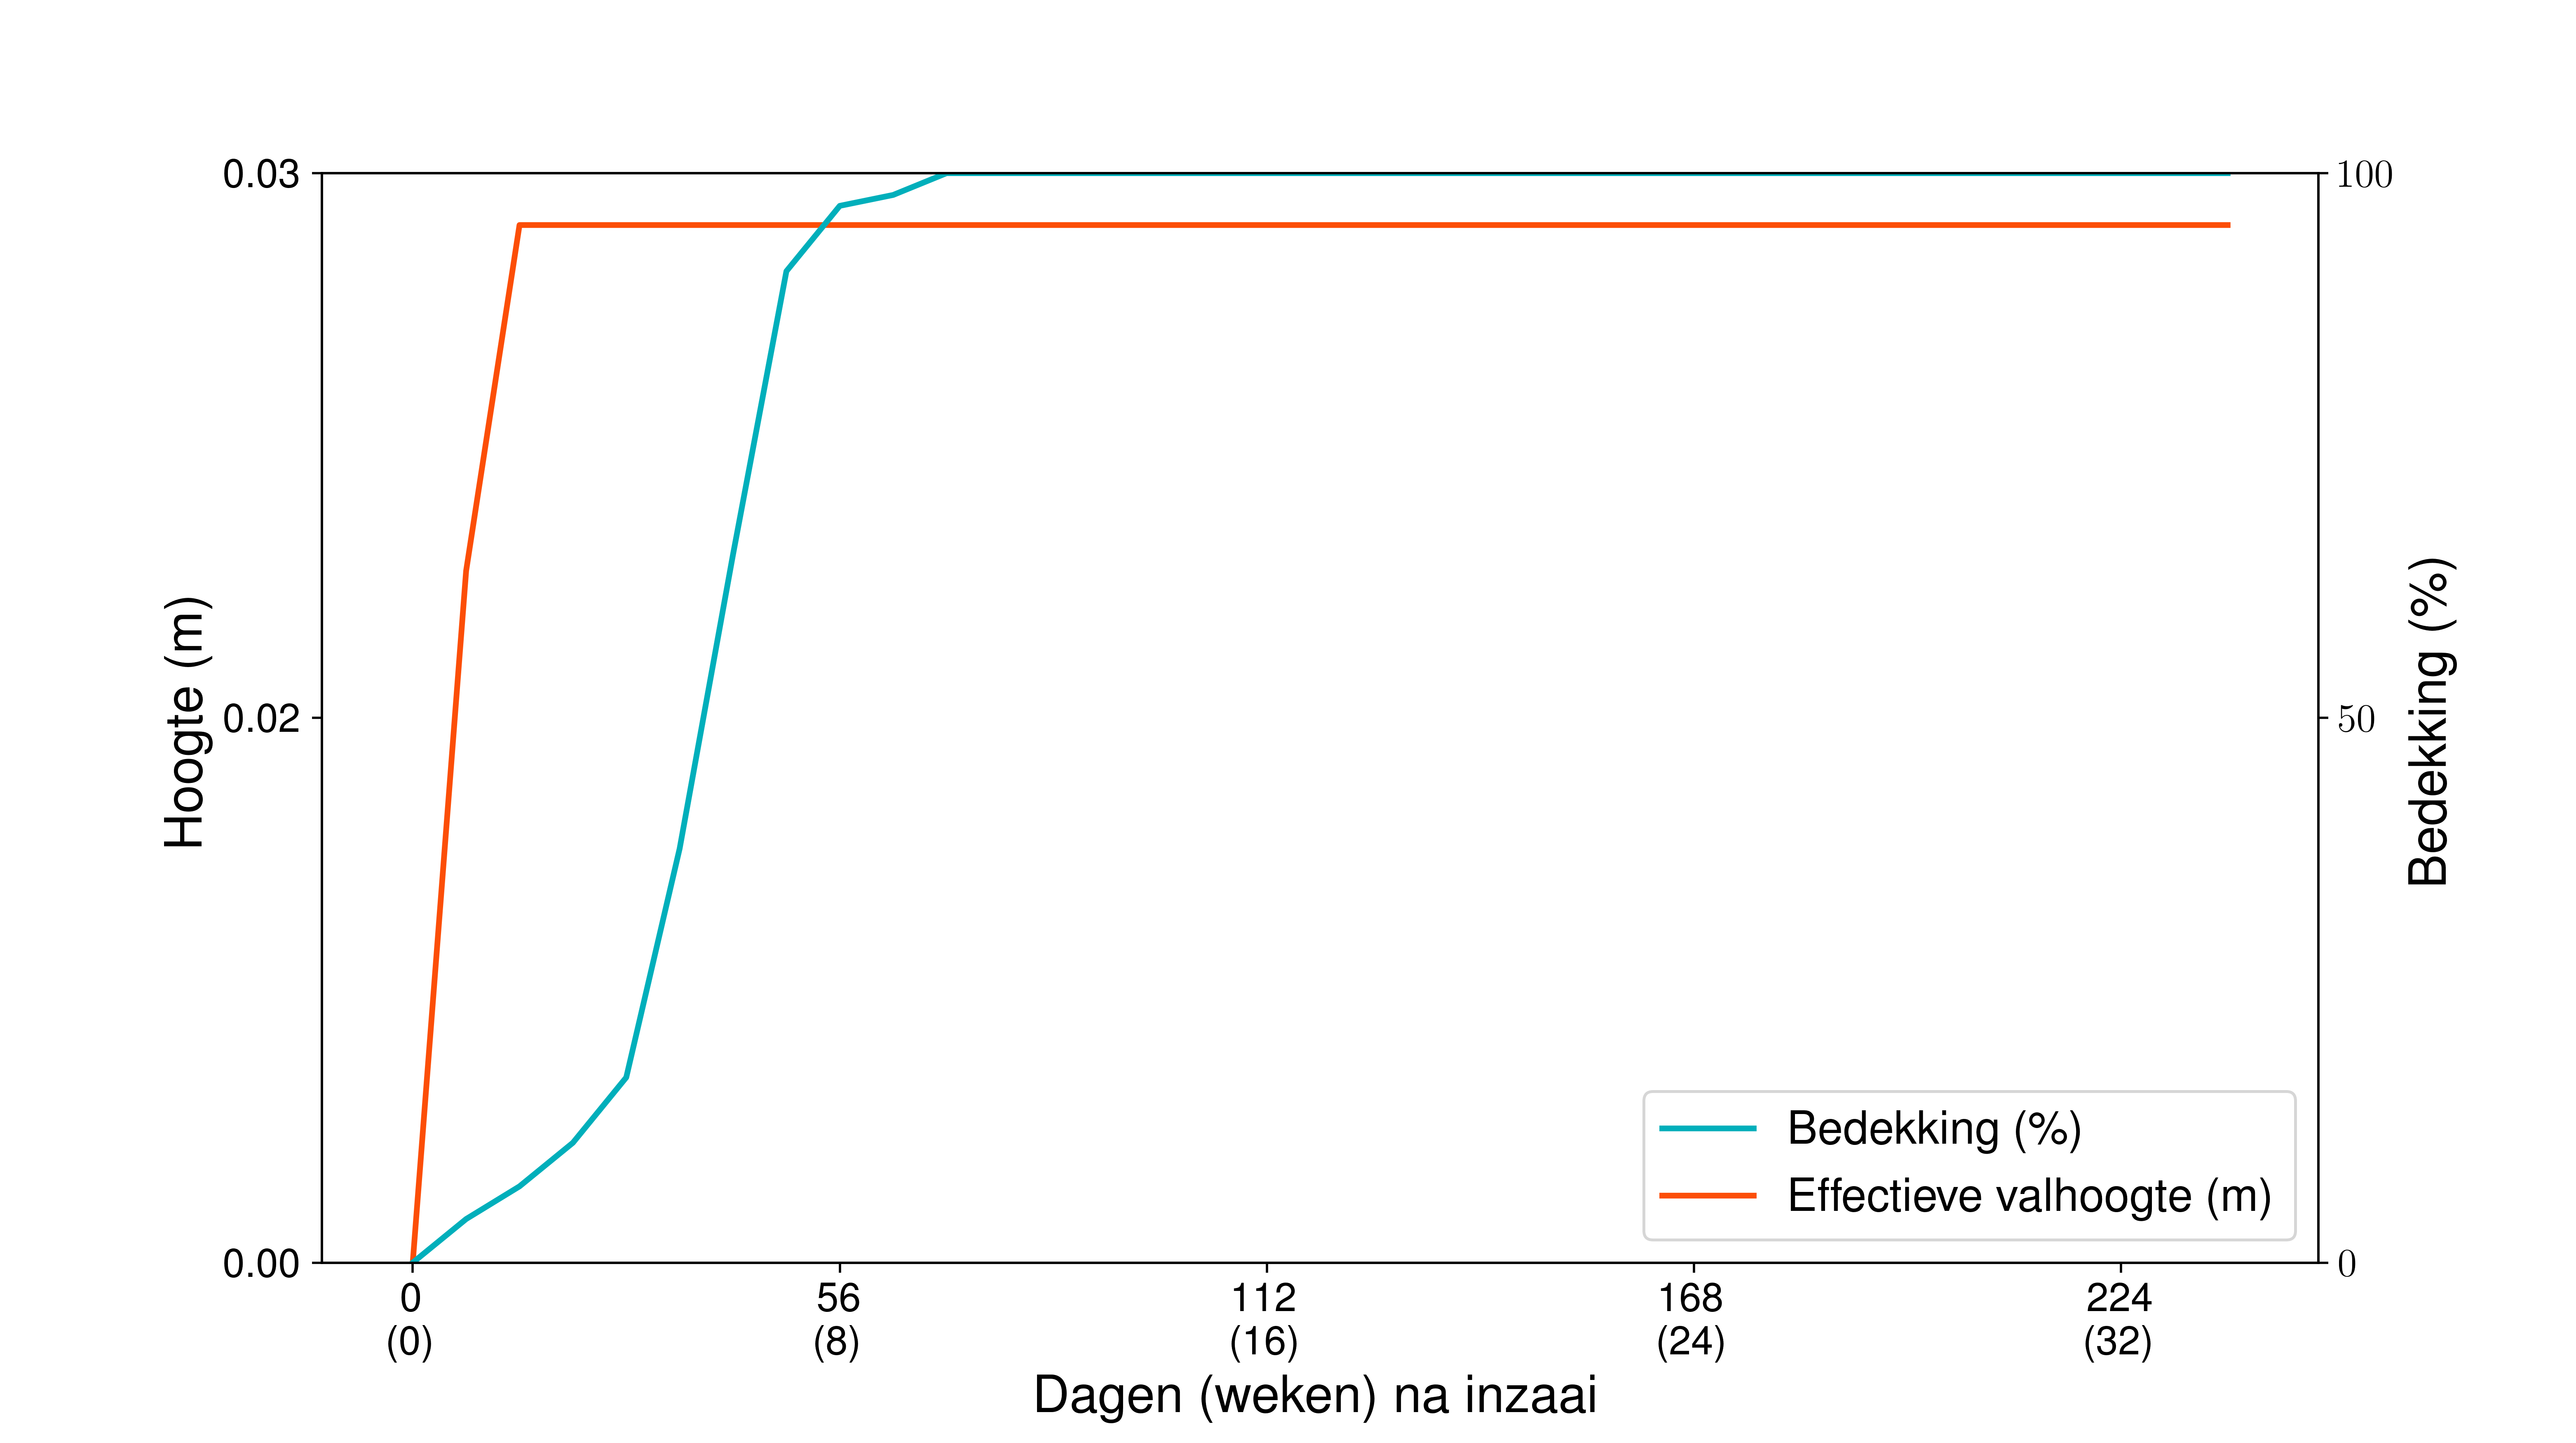
\includegraphics[width=12.5cm]{temp/2016.png} \end{figure} \end{center} 
  \textbf{Referenties:} Gabriels2003;KMI2003;RUSLE;ILVO2019 \vspace{0.10cm} \\ 
  \textbf{Opmerkingen?} geen \vspace{0.10cm} \\ 
 \newpage 
 \subsection{Nateelt (inzaaidatum=[1001,1014]) (subgroep\_id 3016)} 
  \textbf{Zaaidatum (dd/mm)}: 01/10  \vspace{0.10cm} \\ 
  \textbf{Oogstdatum (dd/mm)}: /9  \vspace{0.10cm} \\ 
  \textbf{Oogstresten} \vspace{0.05cm} \\ 
  \tab Initi\"{e}le hoeveelheid (kg ha$^{-1}$): 2500.00 \vspace{0.05cm} \\ 
  \tab Afbraakcoefficient (-): 0.01 \vspace{0.05cm} \\ 
  \tab Bodembedekking (m$^2$ kg$^{-1}$): 11.98 \vspace{0.05cm} \\ 
  \tab Initieel percentage bedekking (\%): 95 \vspace{0.05cm} \\ 
  \tab Halfwaarde tijd (dagen): 30 \vspace{0.05cm} \\ 
  \textbf{Initi\"{e}le bodemruwheid (mm)}: 7.60 \vspace{0.05cm} \\ 
  \textbf{Gewasgroeicurve subgroep\_id 3016:} 
 \begin{center} \begin{figure}[H] 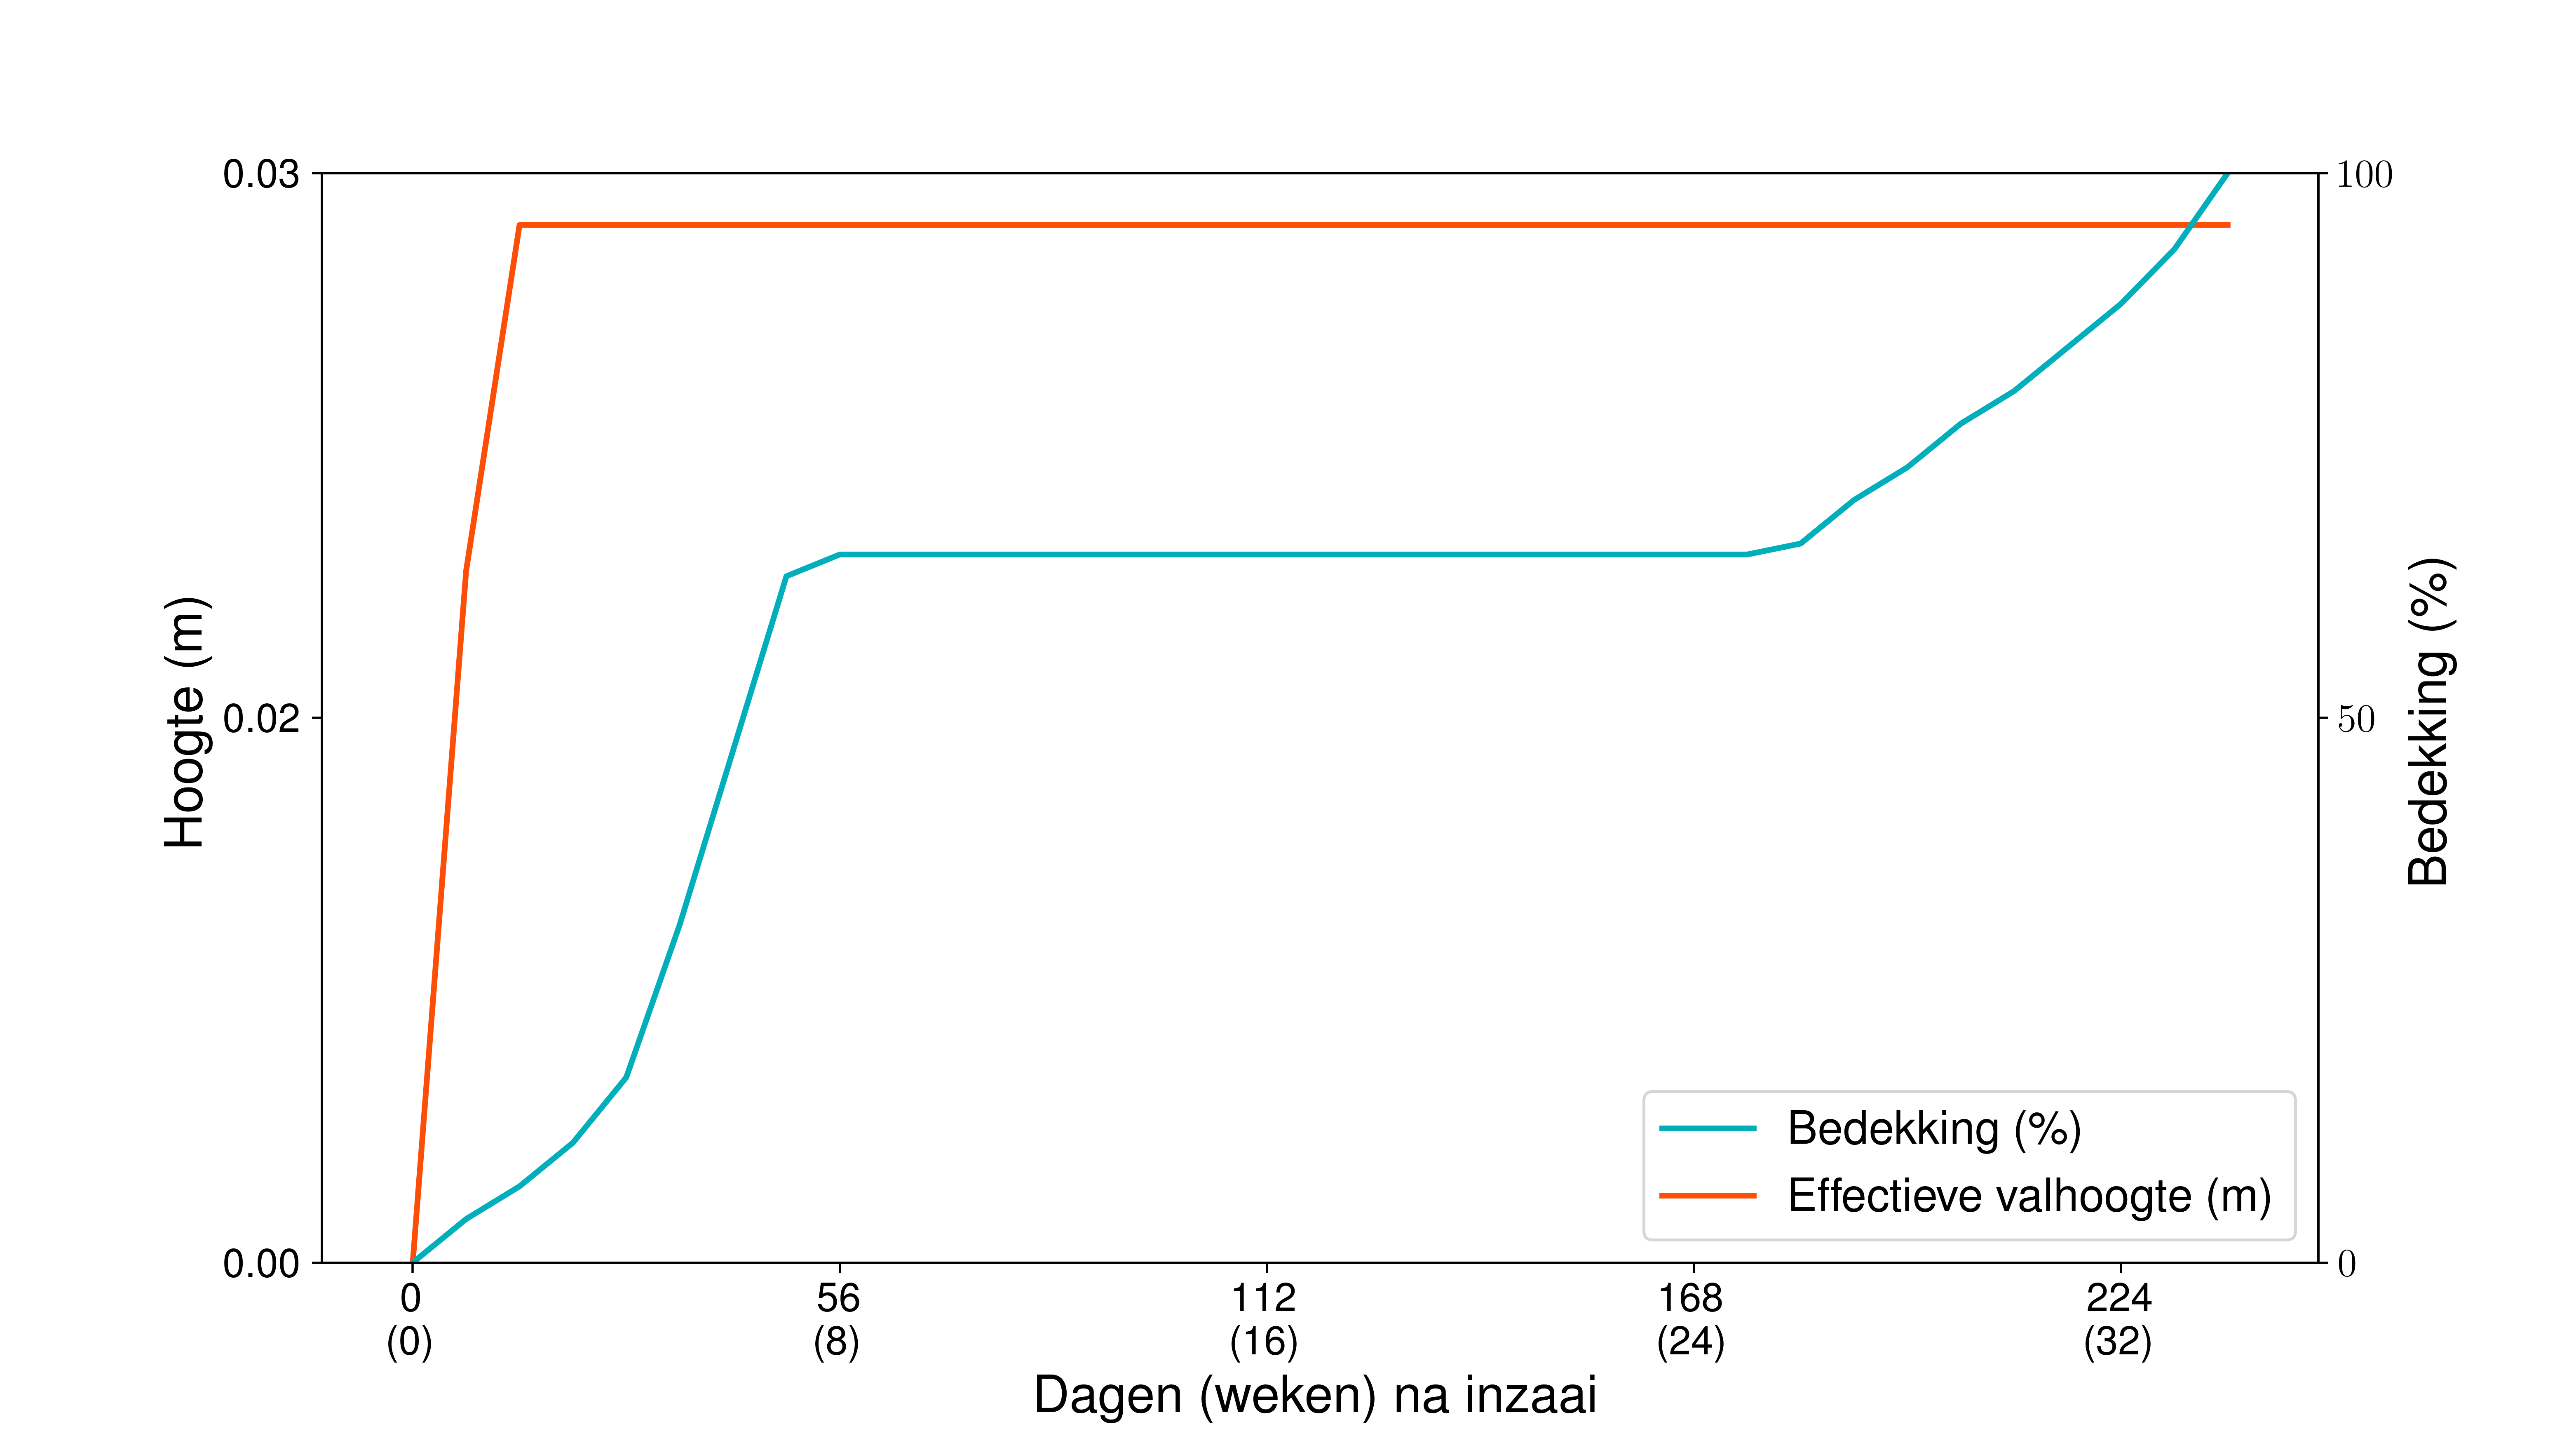
\includegraphics[width=12.5cm]{temp/3016.png} \end{figure} \end{center} 
  \textbf{Referenties:} Gabriels2003;KMI2003;RUSLE;ILVO2019 \vspace{0.10cm} \\ 
  \textbf{Opmerkingen?} geen \vspace{0.10cm} \\ 
 \newpage 
 \subsection{Nateelt (inzaaidatum=[1015,1030]) (subgroep\_id 4016)} 
  \textbf{Zaaidatum (dd/mm)}: 15/10  \vspace{0.10cm} \\ 
  \textbf{Oogstdatum (dd/mm)}: /9  \vspace{0.10cm} \\ 
  \textbf{Oogstresten} \vspace{0.05cm} \\ 
  \tab Initi\"{e}le hoeveelheid (kg ha$^{-1}$): 2500.00 \vspace{0.05cm} \\ 
  \tab Afbraakcoefficient (-): 0.01 \vspace{0.05cm} \\ 
  \tab Bodembedekking (m$^2$ kg$^{-1}$): 11.98 \vspace{0.05cm} \\ 
  \tab Initieel percentage bedekking (\%): 95 \vspace{0.05cm} \\ 
  \tab Halfwaarde tijd (dagen): 30 \vspace{0.05cm} \\ 
  \textbf{Initi\"{e}le bodemruwheid (mm)}: 7.60 \vspace{0.05cm} \\ 
  \textbf{Gewasgroeicurve subgroep\_id 4016:} 
 \begin{center} \begin{figure}[H] 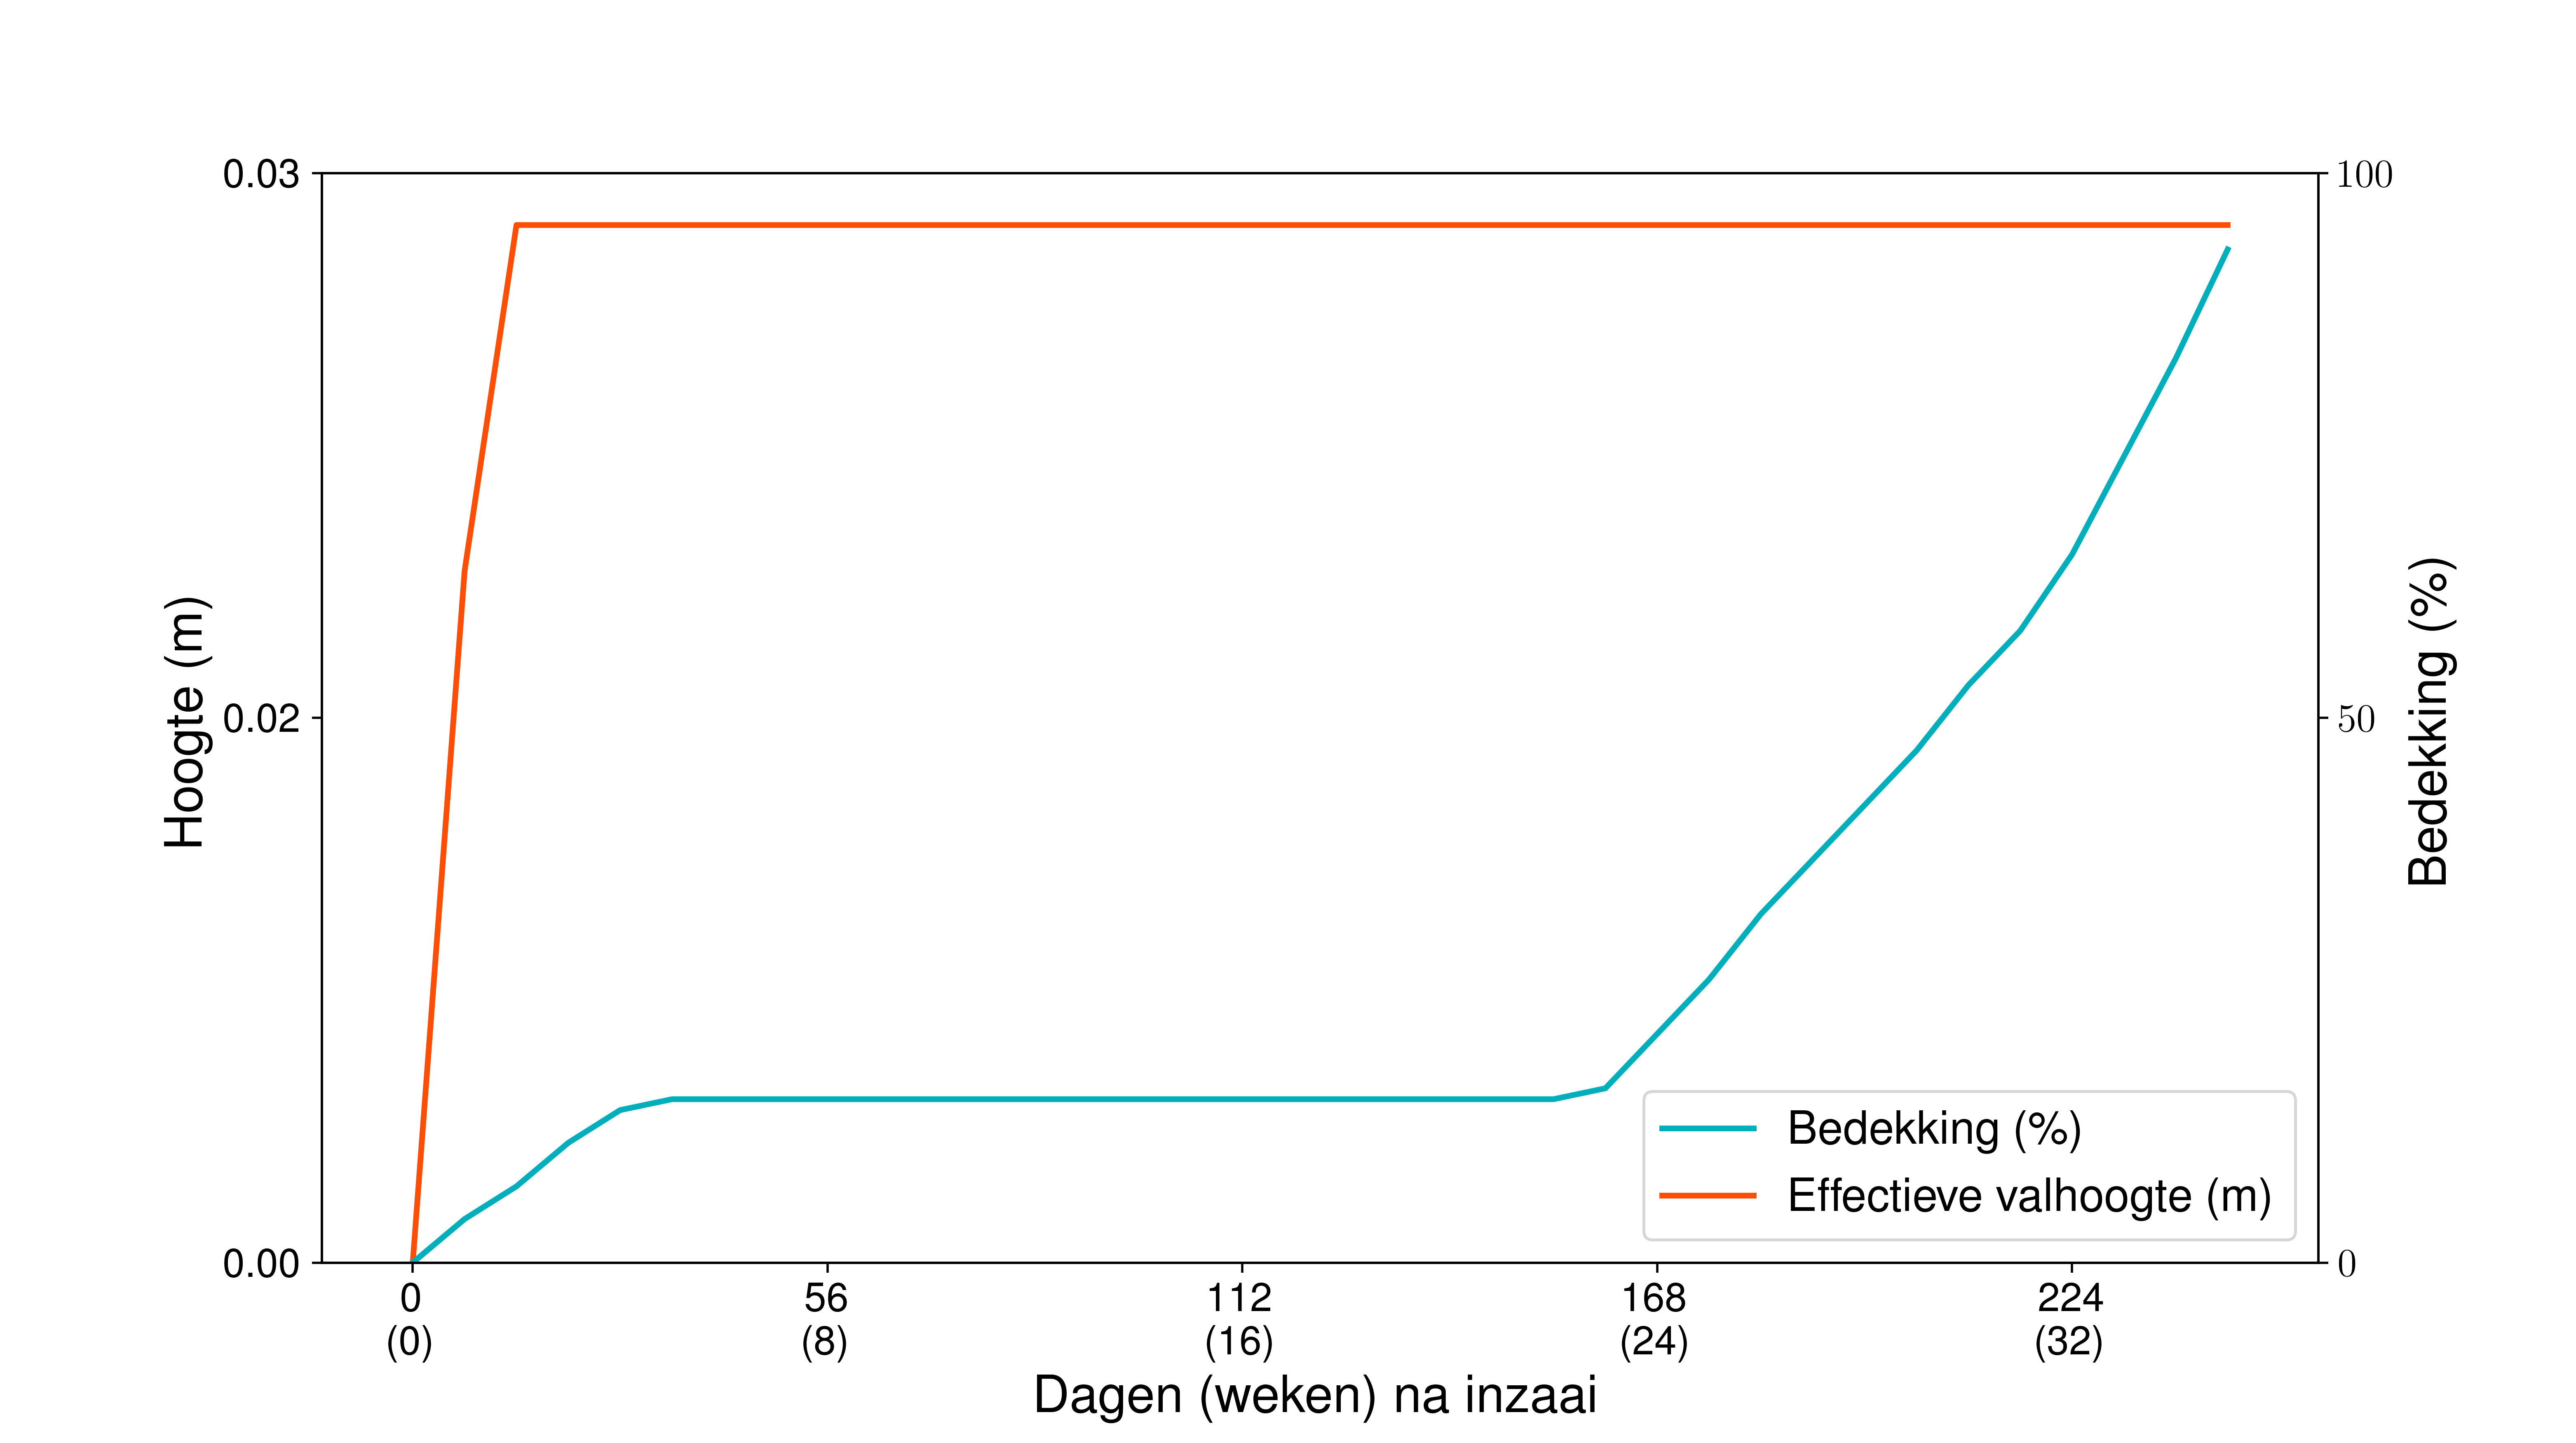
\includegraphics[width=12.5cm]{temp/4016.png} \end{figure} \end{center} 
  \textbf{Referenties:} Gabriels2003;KMI2003;RUSLE;ILVO2019 \vspace{0.10cm} \\ 
  \textbf{Opmerkingen?} geen \vspace{0.10cm} \\ 
 \newpage 
 \subsection{Nateelt (inzaaidatum=[1101,1231]) (subgroep\_id 5016)} 
  \textbf{Zaaidatum (dd/mm)}: 01/11  \vspace{0.10cm} \\ 
  \textbf{Oogstdatum (dd/mm)}: /9  \vspace{0.10cm} \\ 
  \textbf{Oogstresten} \vspace{0.05cm} \\ 
  \tab Initi\"{e}le hoeveelheid (kg ha$^{-1}$): 2500.00 \vspace{0.05cm} \\ 
  \tab Afbraakcoefficient (-): 0.01 \vspace{0.05cm} \\ 
  \tab Bodembedekking (m$^2$ kg$^{-1}$): 11.98 \vspace{0.05cm} \\ 
  \tab Initieel percentage bedekking (\%): 95 \vspace{0.05cm} \\ 
  \tab Halfwaarde tijd (dagen): 30 \vspace{0.05cm} \\ 
  \textbf{Initi\"{e}le bodemruwheid (mm)}: 7.60 \vspace{0.05cm} \\ 
  \textbf{Gewasgroeicurve subgroep\_id 5016:} 
 \begin{center} \begin{figure}[H] 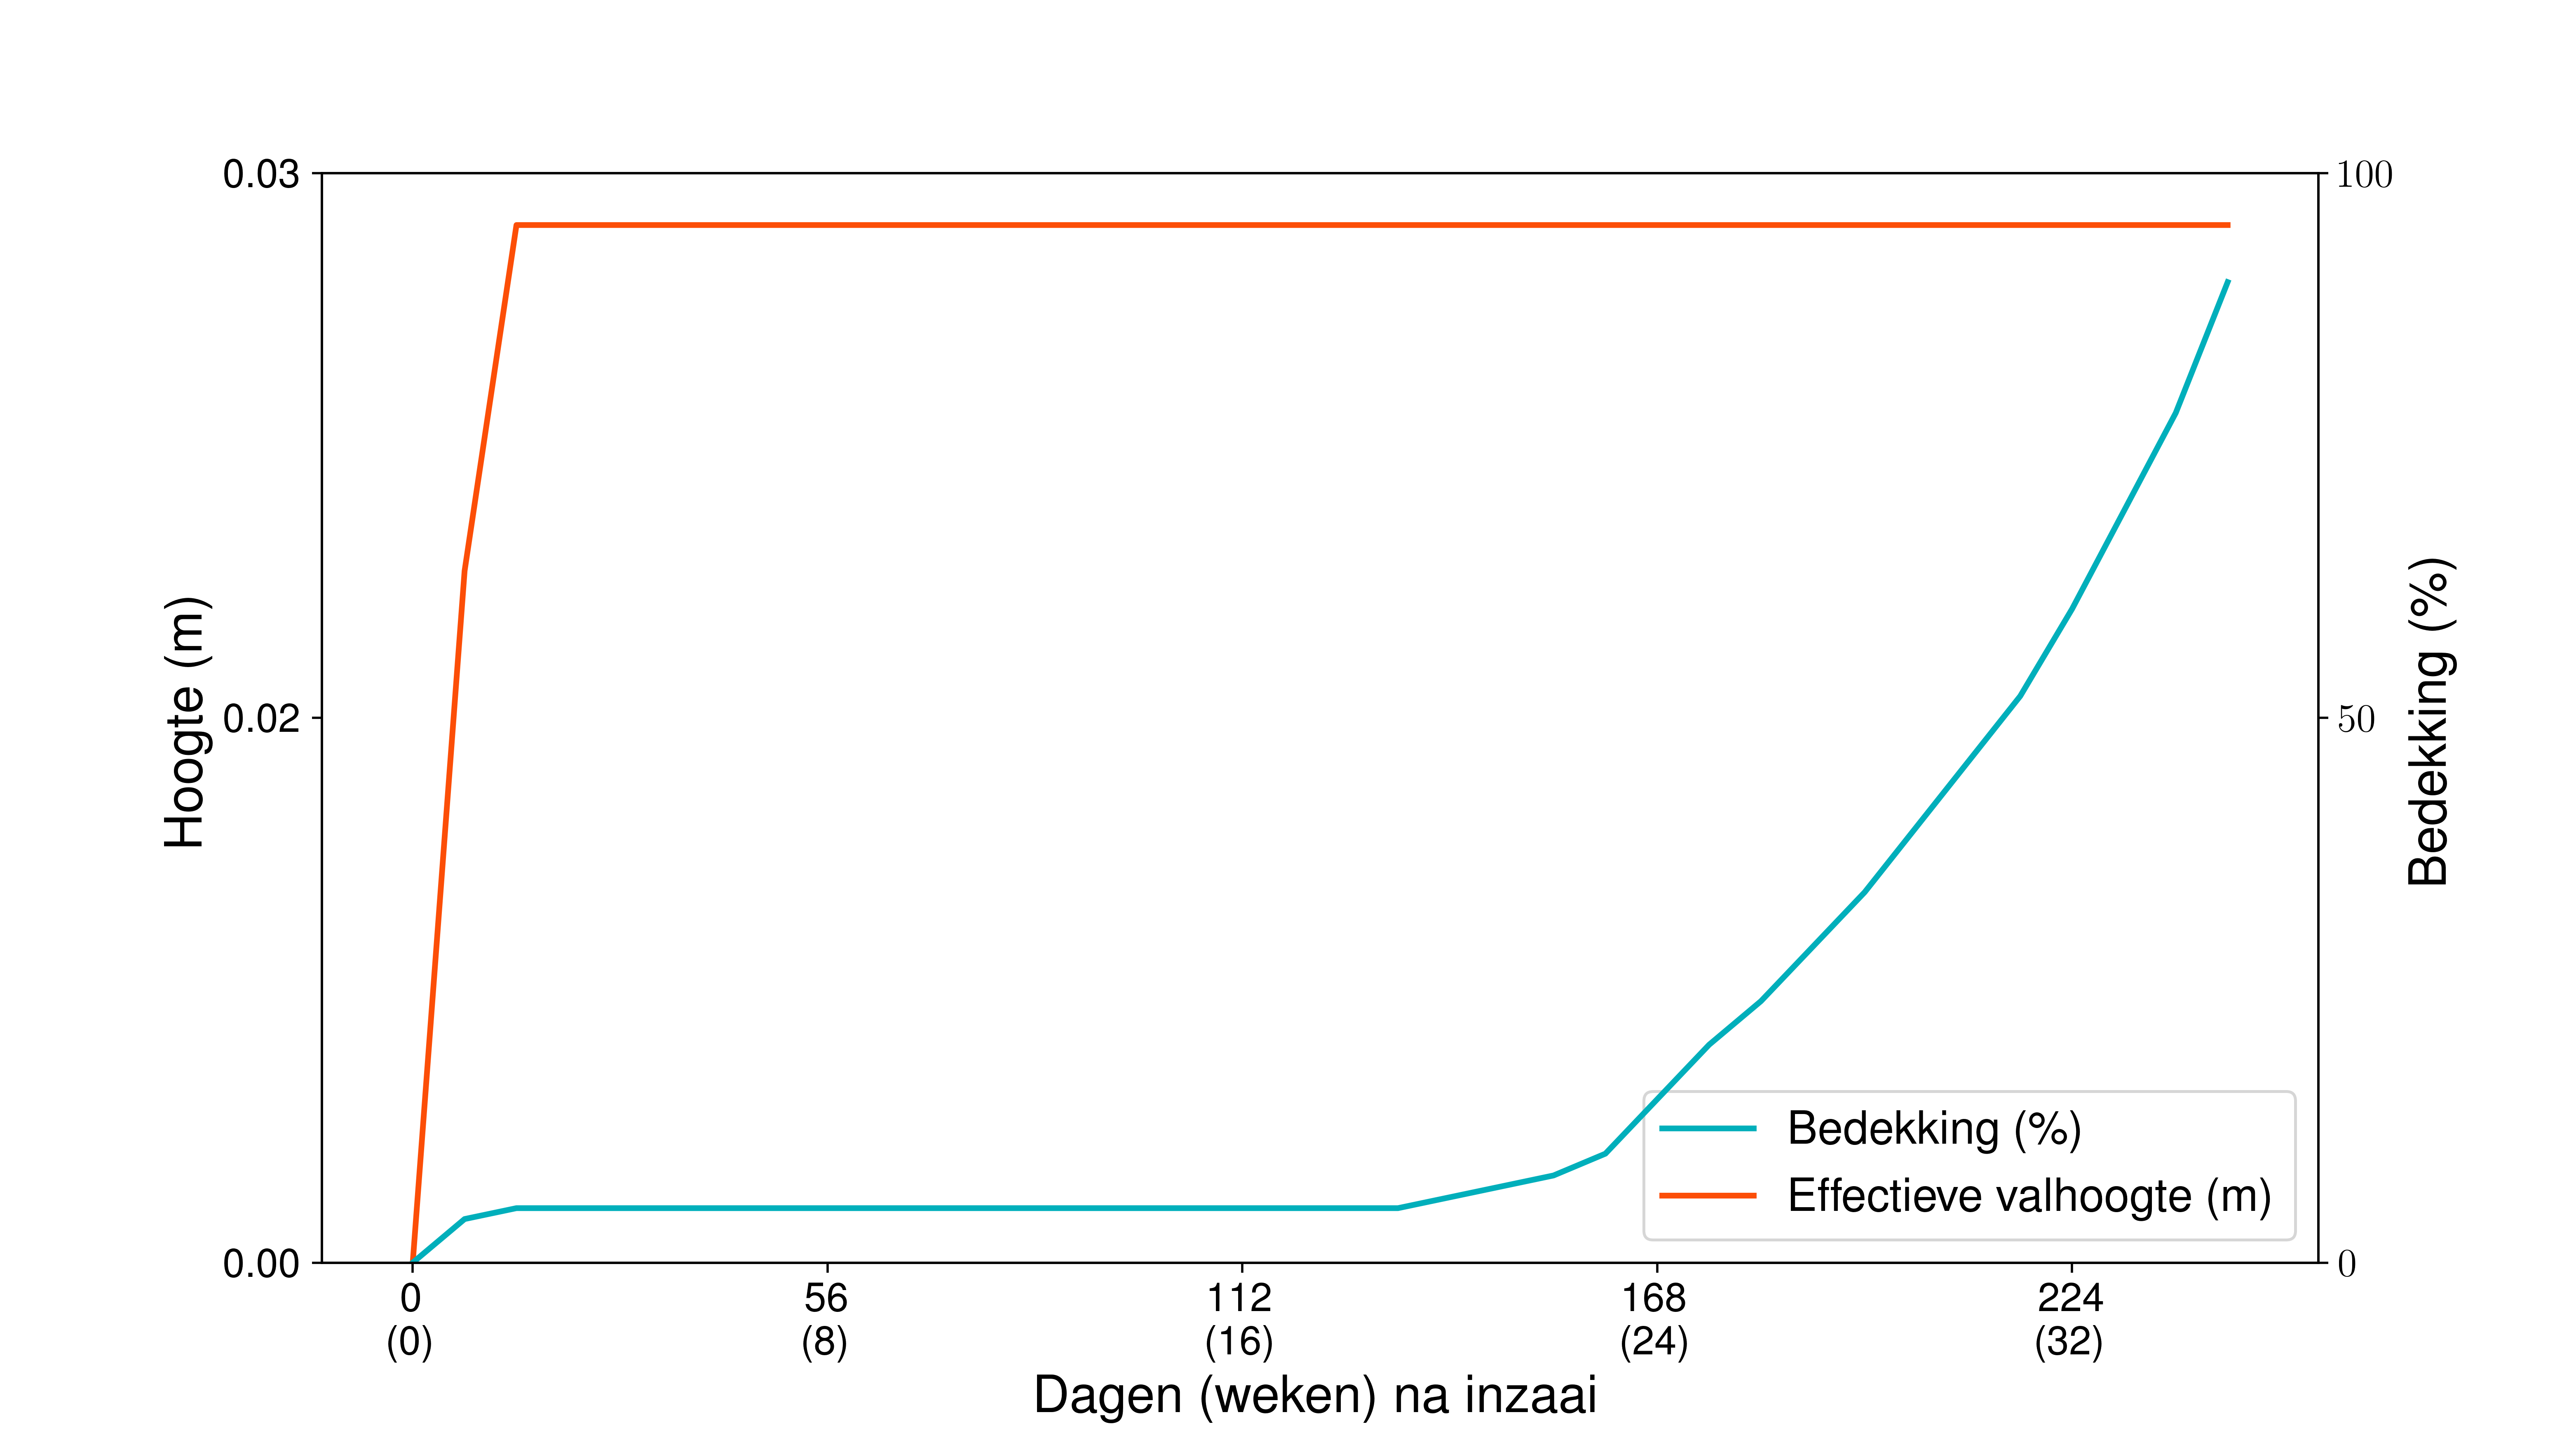
\includegraphics[width=12.5cm]{temp/5016.png} \end{figure} \end{center} 
  \textbf{Referenties:} Gabriels2003;KMI2003;RUSLE;ILVO2019 \vspace{0.10cm} \\ 
  \textbf{Opmerkingen?} geen \vspace{0.10cm} \\ 
 \newpage 
 \section{Italiaans raaigras (groep\_id 17)} 
 \textbf{Van toepassing op gewasnamen (en codes):} Italiaans raaigras (634) , Snijrogge (639) 
 \begin{multicols}{3} \begin{itemize} \item[$\boxtimes$] Meerjarig \item[$\boxtimes$] Groenbedekker \item[$\square$] Groente \end{itemize} \end{multicols} 
 \subsection{Hoofdteelt, voorteelt en nateelt (inzaaidatum=[0901,0930]) (subgroep\_id 2016)} 
  \textbf{Zaaidatum (dd/mm)}: 01/09  \vspace{0.10cm} \\ 
  \textbf{Oogstdatum (dd/mm)}: /9  \vspace{0.10cm} \\ 
  \textbf{Oogstresten} \vspace{0.05cm} \\ 
  \tab Initi\"{e}le hoeveelheid (kg ha$^{-1}$): 2500.00 \vspace{0.05cm} \\ 
  \tab Afbraakcoefficient (-): 0.01 \vspace{0.05cm} \\ 
  \tab Bodembedekking (m$^2$ kg$^{-1}$): 11.98 \vspace{0.05cm} \\ 
  \tab Initieel percentage bedekking (\%): 95 \vspace{0.05cm} \\ 
  \tab Halfwaarde tijd (dagen): 30 \vspace{0.05cm} \\ 
  \textbf{Initi\"{e}le bodemruwheid (mm)}: 7.60 \vspace{0.05cm} \\ 
  \textbf{Gewasgroeicurve subgroep\_id 2016:} 
 \begin{center} \begin{figure}[H] 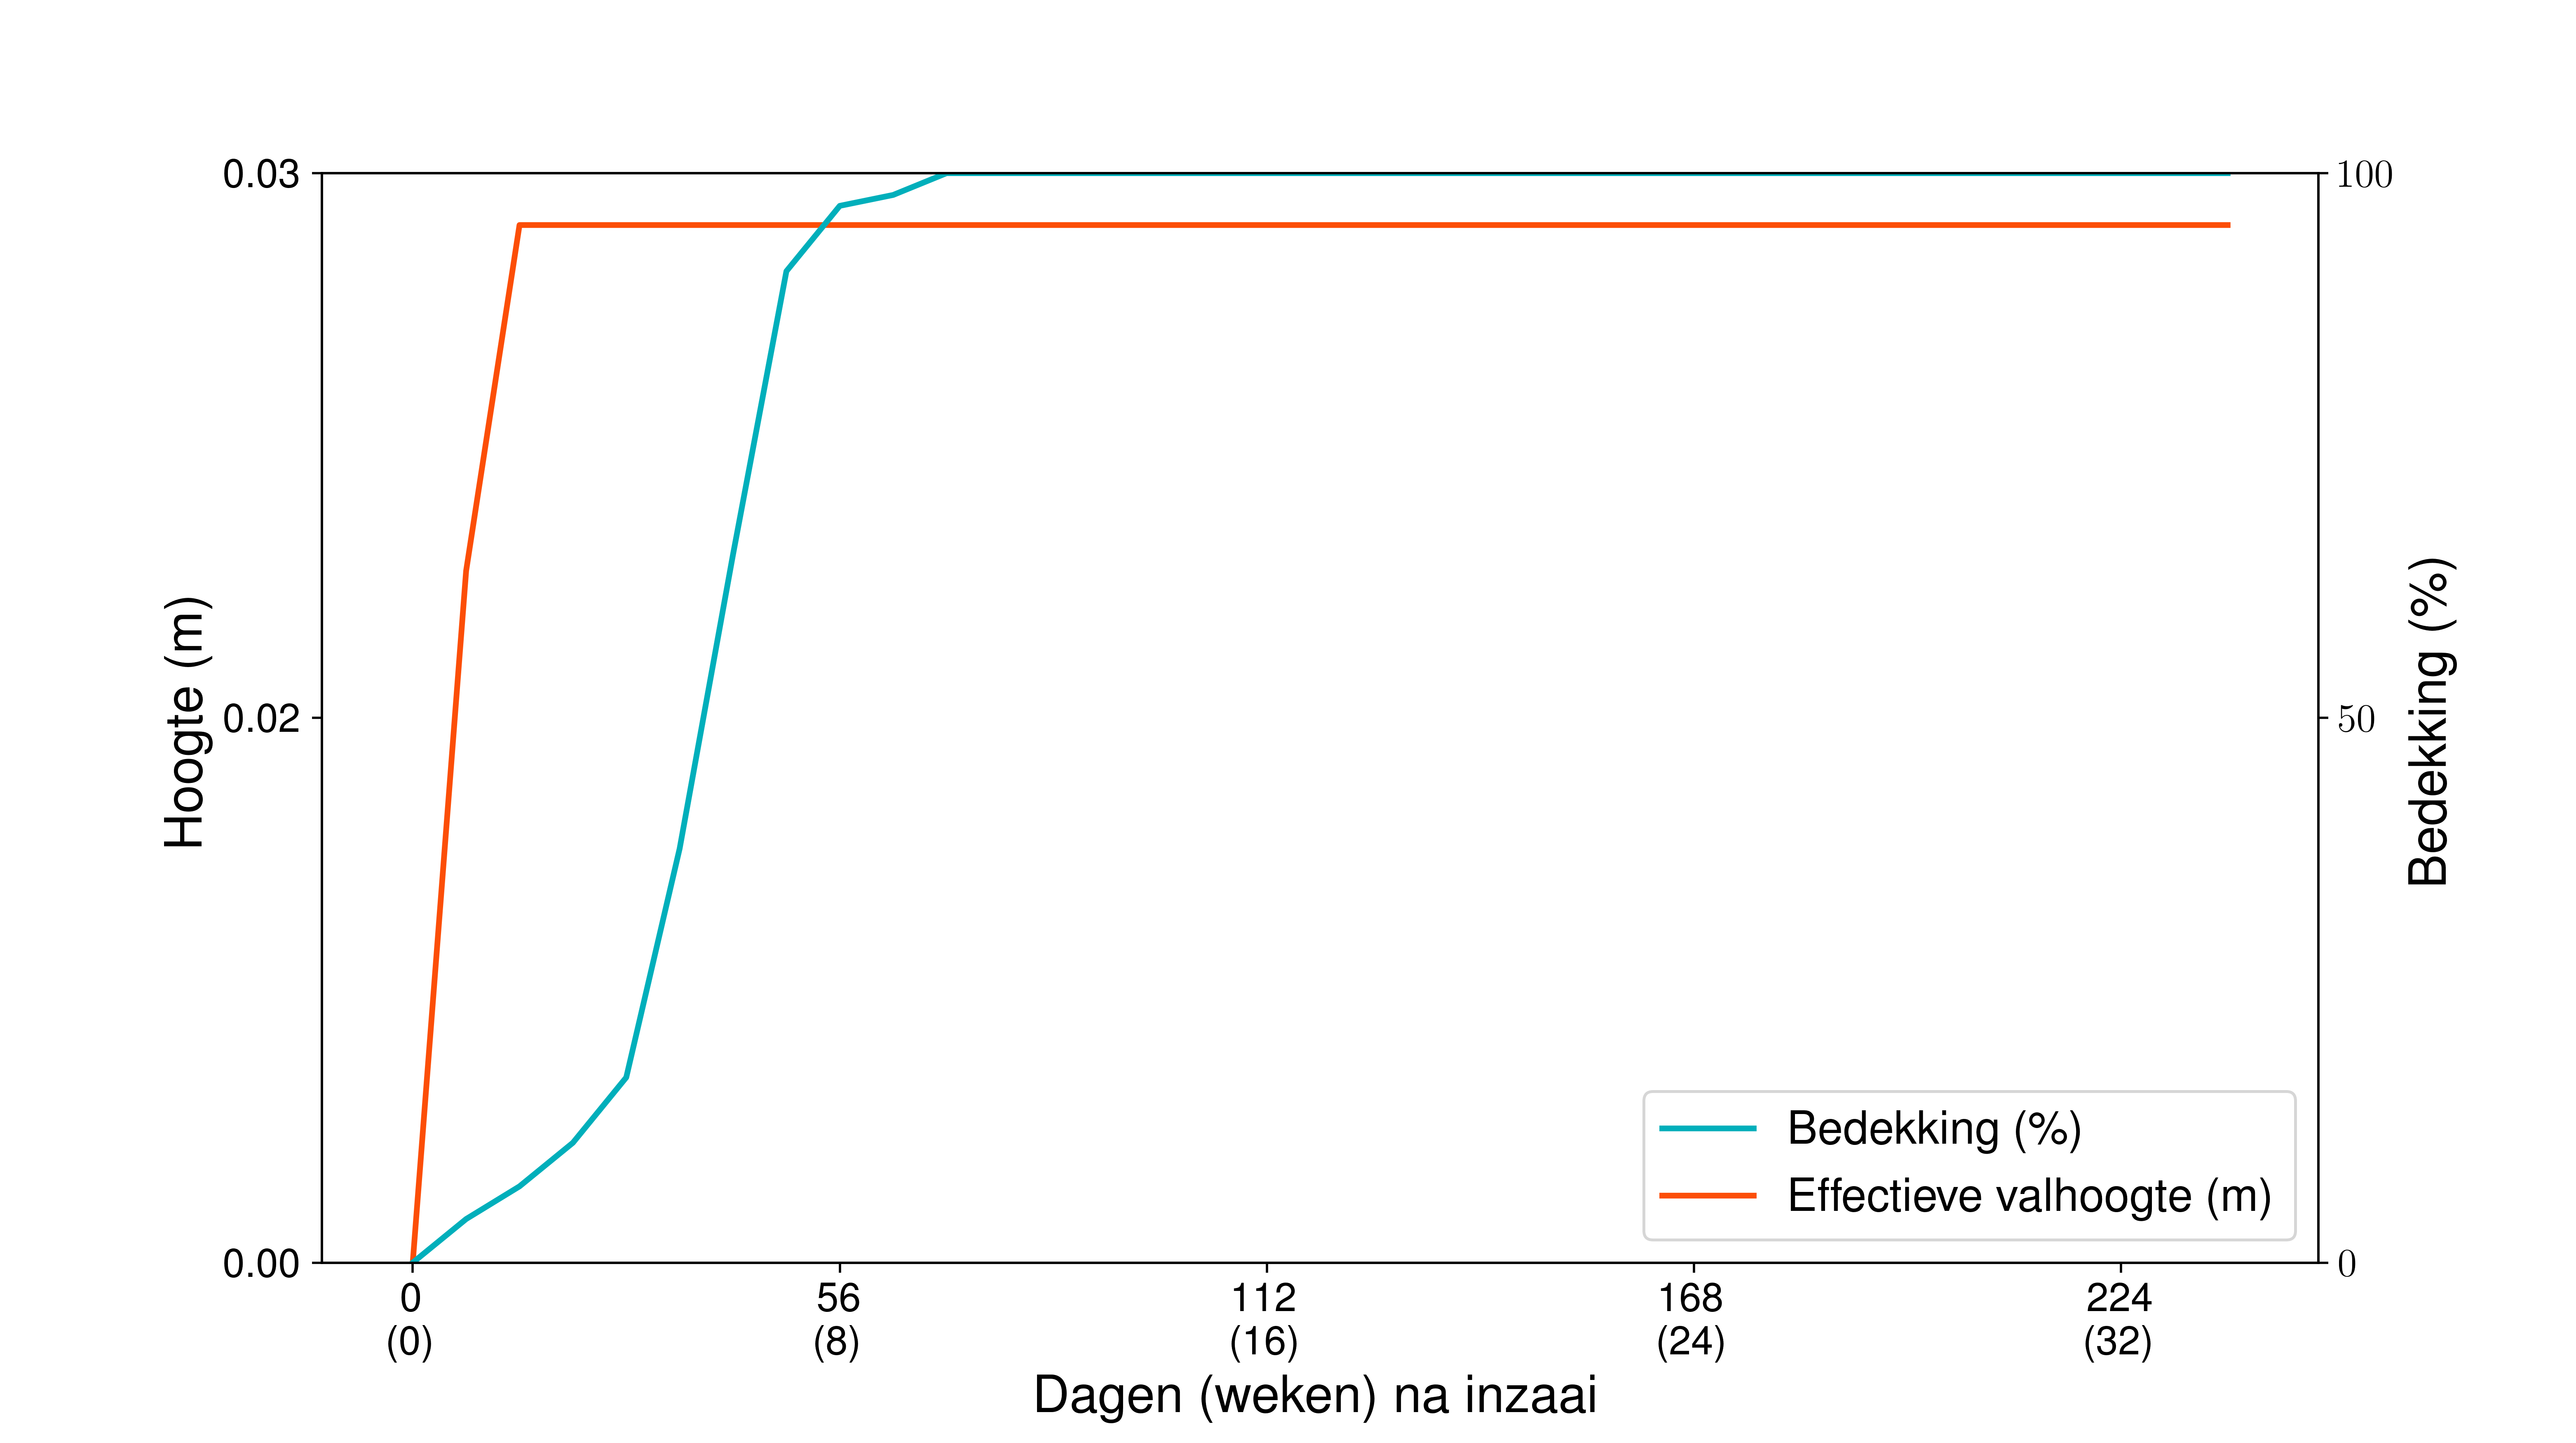
\includegraphics[width=12.5cm]{temp/2016.png} \end{figure} \end{center} 
  \textbf{Referenties:} Gabriels2003;KMI2003;RUSLE;ILVO2019 \vspace{0.10cm} \\ 
  \textbf{Opmerkingen?} geen \vspace{0.10cm} \\ 
 \newpage 
 \subsection{Hoofdteelt, voorteelt en nateelt (inzaaidatum=[1001,1014]) (subgroep\_id 3016)} 
  \textbf{Zaaidatum (dd/mm)}: 01/10  \vspace{0.10cm} \\ 
  \textbf{Oogstdatum (dd/mm)}: /9  \vspace{0.10cm} \\ 
  \textbf{Oogstresten} \vspace{0.05cm} \\ 
  \tab Initi\"{e}le hoeveelheid (kg ha$^{-1}$): 2500.00 \vspace{0.05cm} \\ 
  \tab Afbraakcoefficient (-): 0.01 \vspace{0.05cm} \\ 
  \tab Bodembedekking (m$^2$ kg$^{-1}$): 11.98 \vspace{0.05cm} \\ 
  \tab Initieel percentage bedekking (\%): 95 \vspace{0.05cm} \\ 
  \tab Halfwaarde tijd (dagen): 30 \vspace{0.05cm} \\ 
  \textbf{Initi\"{e}le bodemruwheid (mm)}: 7.60 \vspace{0.05cm} \\ 
  \textbf{Gewasgroeicurve subgroep\_id 3016:} 
 \begin{center} \begin{figure}[H] 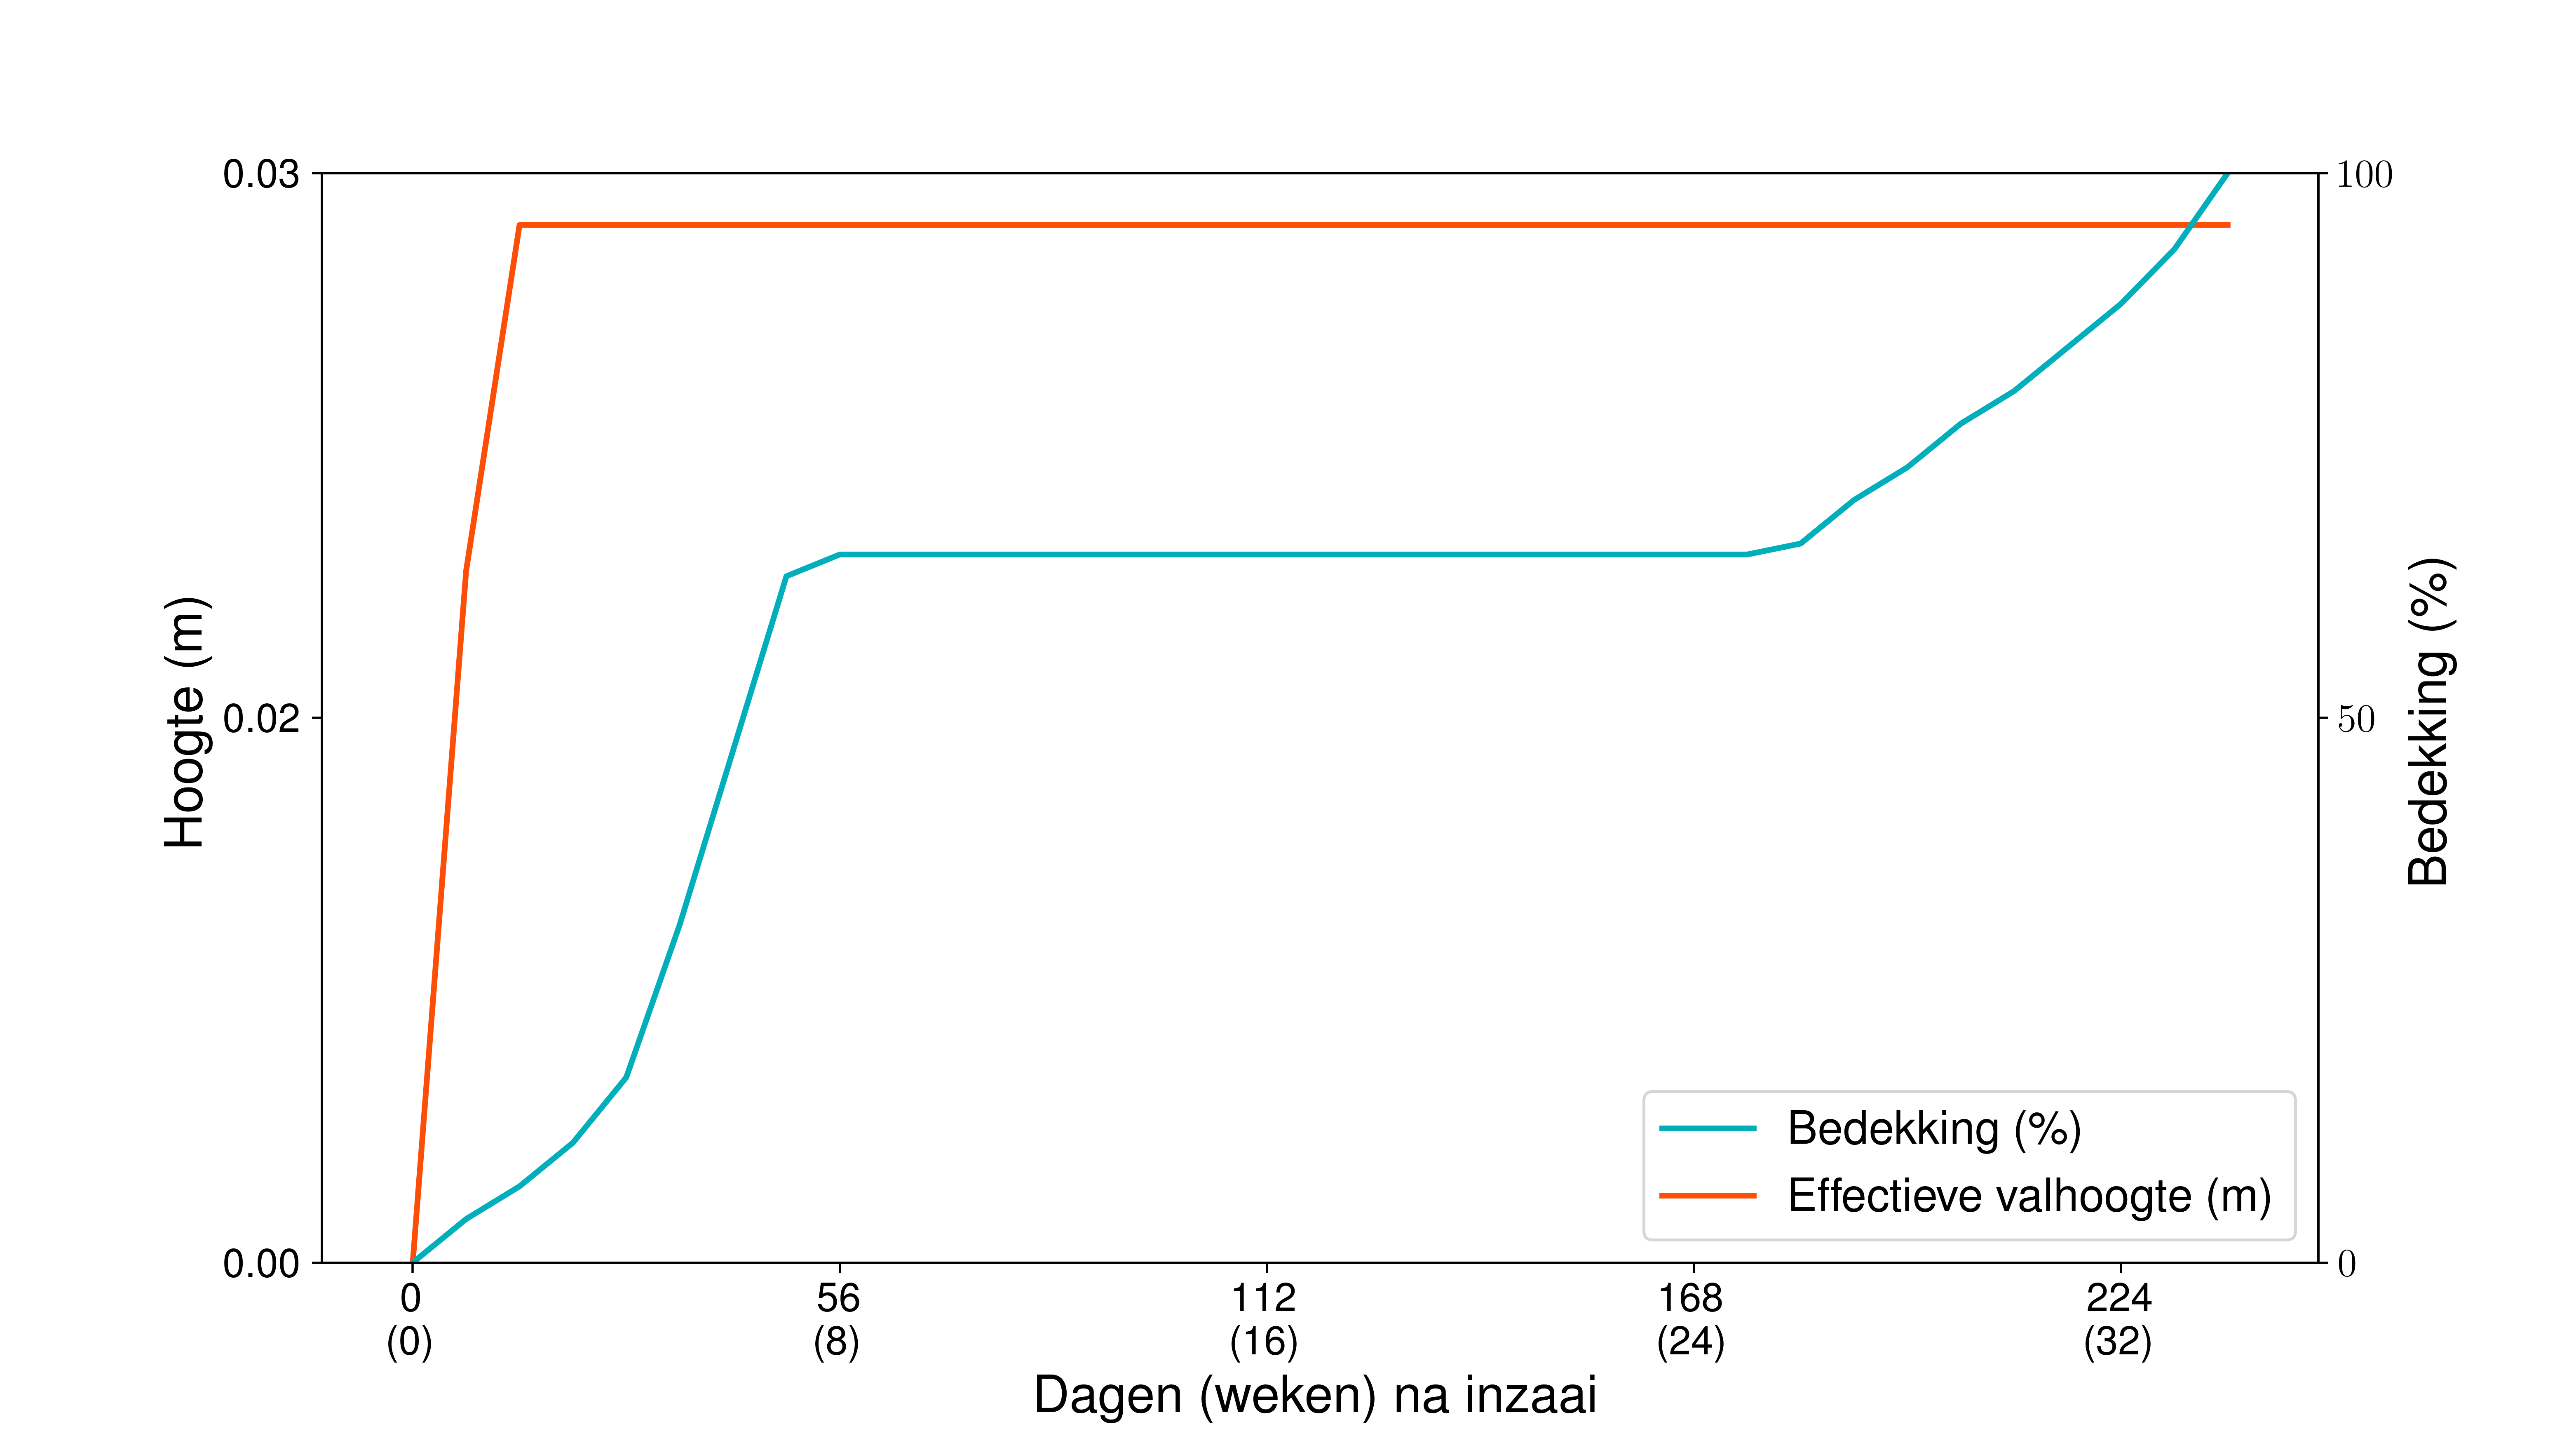
\includegraphics[width=12.5cm]{temp/3016.png} \end{figure} \end{center} 
  \textbf{Referenties:} Gabriels2003;KMI2003;RUSLE;ILVO2019 \vspace{0.10cm} \\ 
  \textbf{Opmerkingen?} geen \vspace{0.10cm} \\ 
 \newpage 
 \subsection{Hoofdteelt, voorteelt en nateelt (inzaaidatum=[1015,1030]) (subgroep\_id 4016)} 
  \textbf{Zaaidatum (dd/mm)}: 15/10  \vspace{0.10cm} \\ 
  \textbf{Oogstdatum (dd/mm)}: /9  \vspace{0.10cm} \\ 
  \textbf{Oogstresten} \vspace{0.05cm} \\ 
  \tab Initi\"{e}le hoeveelheid (kg ha$^{-1}$): 2500.00 \vspace{0.05cm} \\ 
  \tab Afbraakcoefficient (-): 0.01 \vspace{0.05cm} \\ 
  \tab Bodembedekking (m$^2$ kg$^{-1}$): 11.98 \vspace{0.05cm} \\ 
  \tab Initieel percentage bedekking (\%): 95 \vspace{0.05cm} \\ 
  \tab Halfwaarde tijd (dagen): 30 \vspace{0.05cm} \\ 
  \textbf{Initi\"{e}le bodemruwheid (mm)}: 7.60 \vspace{0.05cm} \\ 
  \textbf{Gewasgroeicurve subgroep\_id 4016:} 
 \begin{center} \begin{figure}[H] 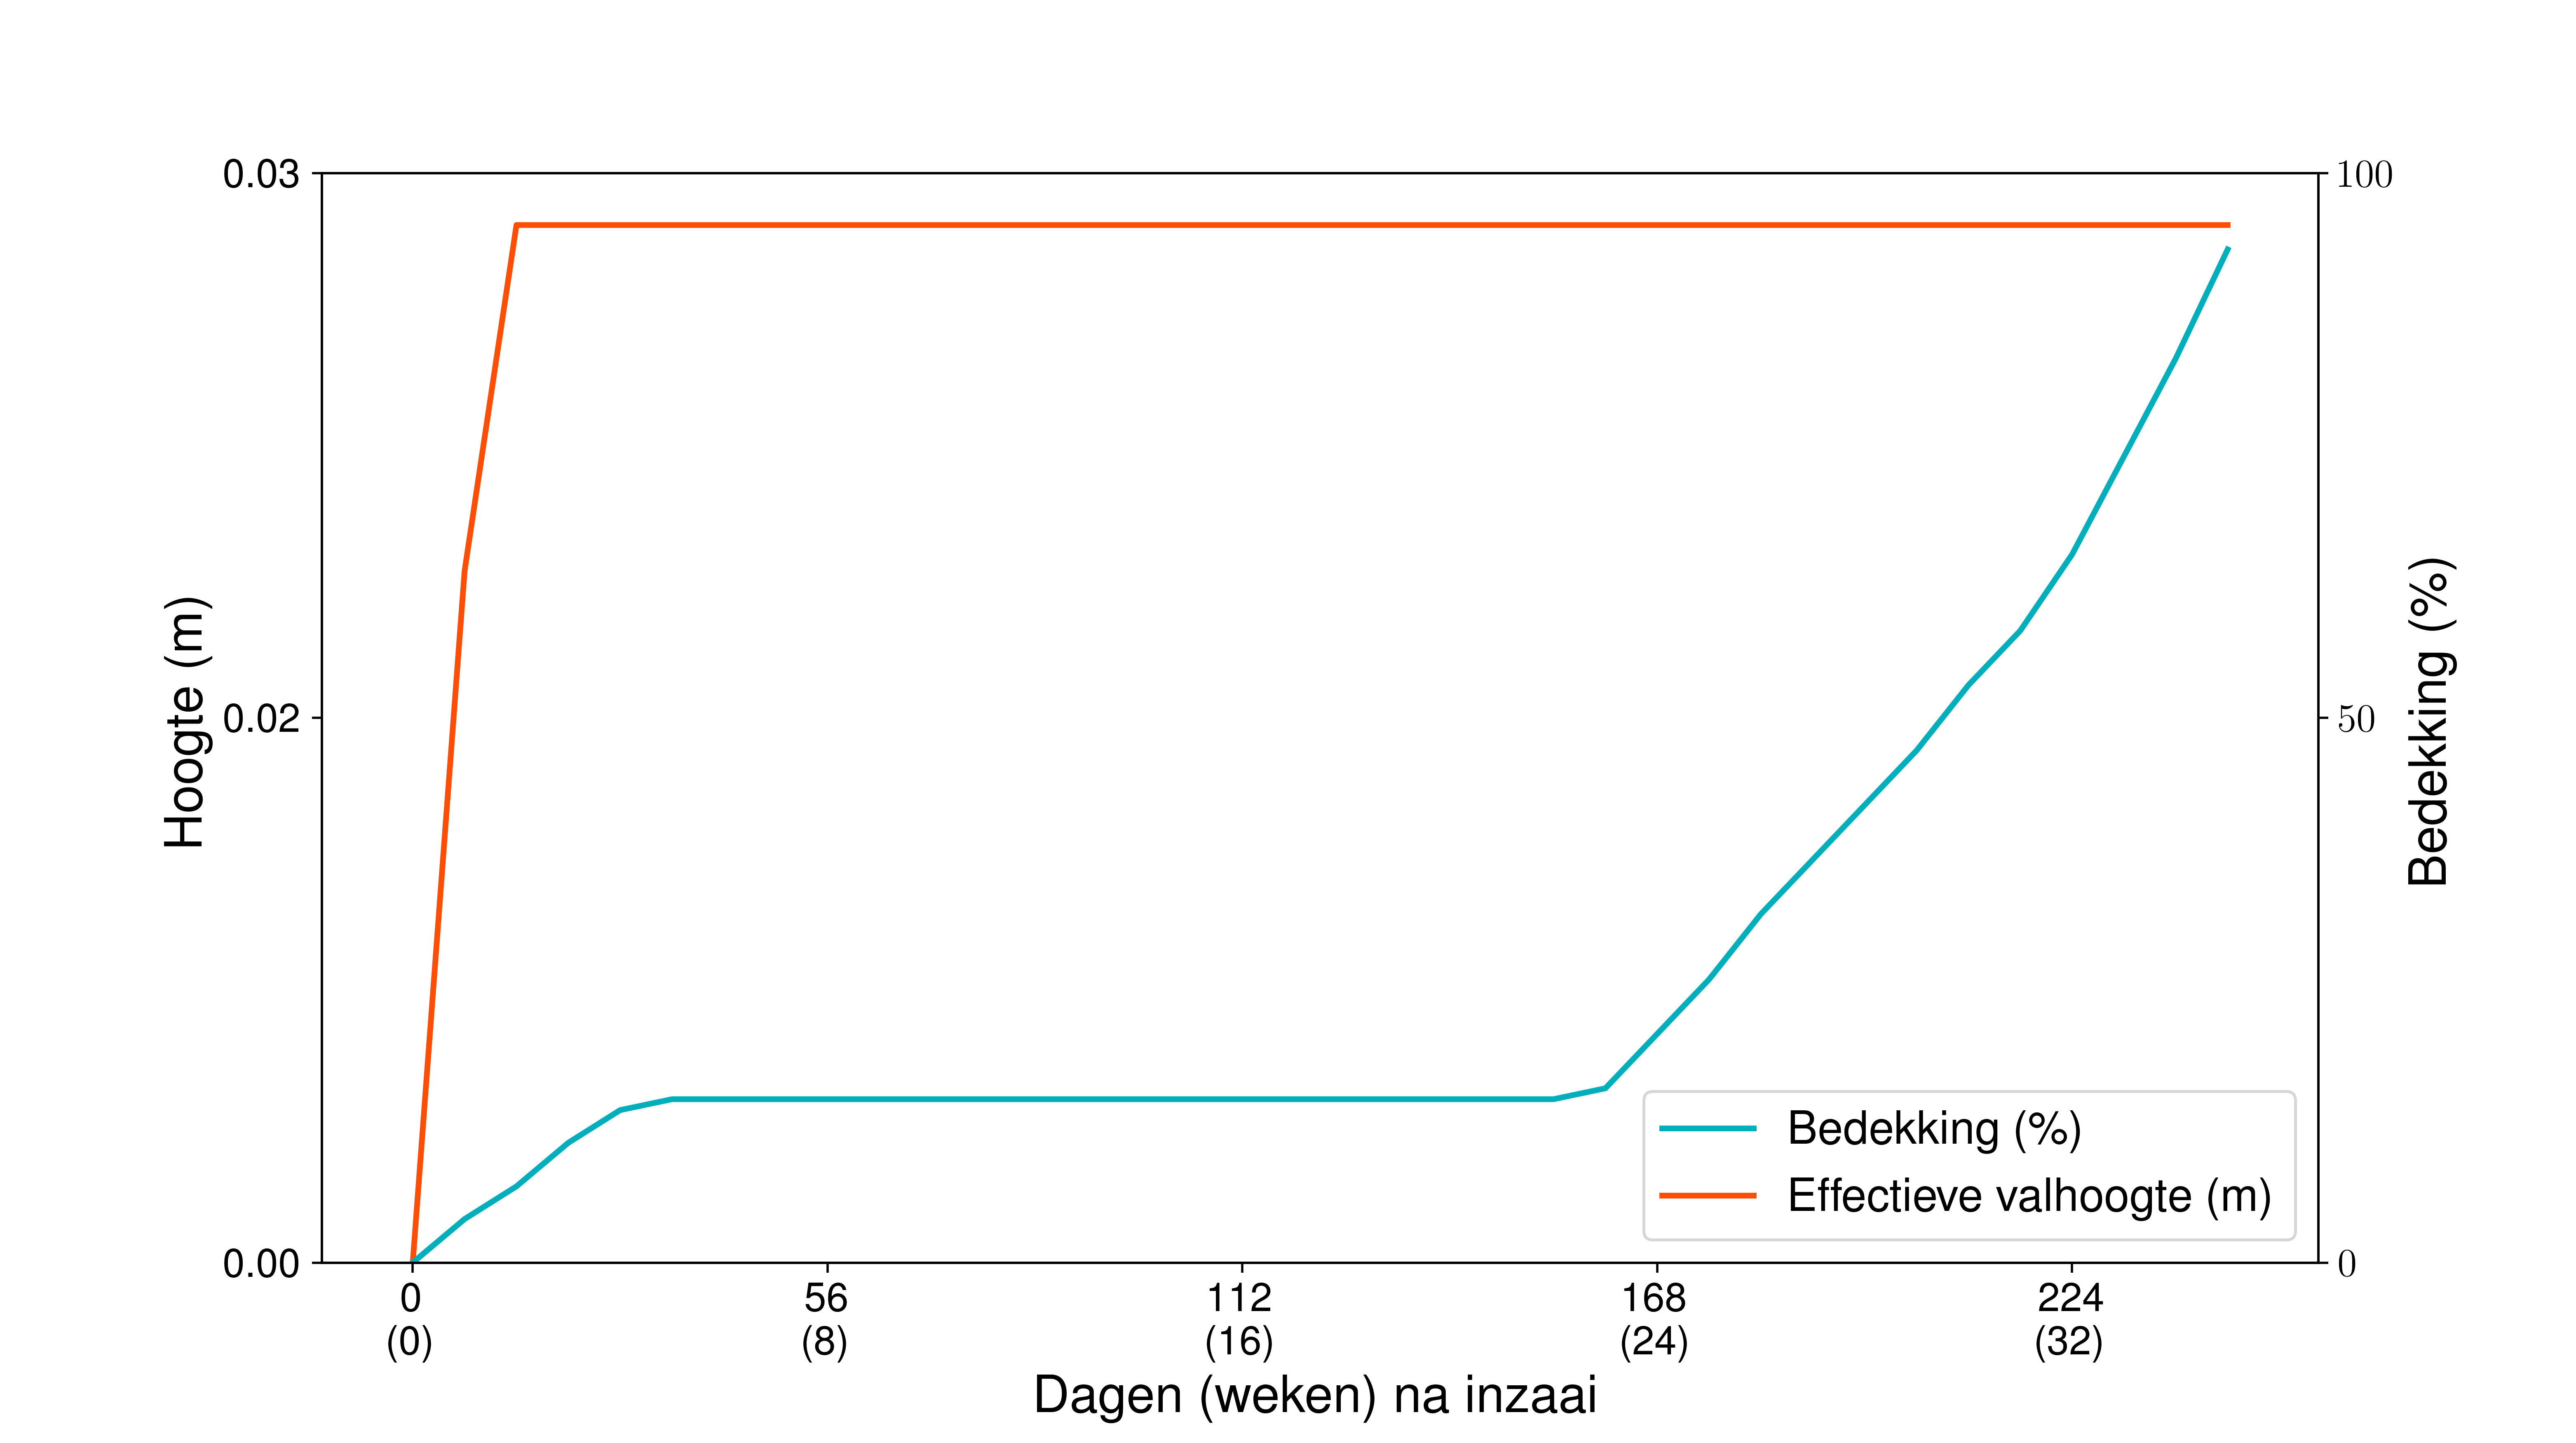
\includegraphics[width=12.5cm]{temp/4016.png} \end{figure} \end{center} 
  \textbf{Referenties:} Gabriels2003;KMI2003;RUSLE;ILVO2019 \vspace{0.10cm} \\ 
  \textbf{Opmerkingen?} geen \vspace{0.10cm} \\ 
 \newpage 
 \subsection{Hoofdteelt, voorteelt en nateelt (inzaaidatum=[1101,1231]) (subgroep\_id 5016)} 
  \textbf{Zaaidatum (dd/mm)}: 01/11  \vspace{0.10cm} \\ 
  \textbf{Oogstdatum (dd/mm)}: /9  \vspace{0.10cm} \\ 
  \textbf{Oogstresten} \vspace{0.05cm} \\ 
  \tab Initi\"{e}le hoeveelheid (kg ha$^{-1}$): 2500.00 \vspace{0.05cm} \\ 
  \tab Afbraakcoefficient (-): 0.01 \vspace{0.05cm} \\ 
  \tab Bodembedekking (m$^2$ kg$^{-1}$): 11.98 \vspace{0.05cm} \\ 
  \tab Initieel percentage bedekking (\%): 95 \vspace{0.05cm} \\ 
  \tab Halfwaarde tijd (dagen): 30 \vspace{0.05cm} \\ 
  \textbf{Initi\"{e}le bodemruwheid (mm)}: 7.60 \vspace{0.05cm} \\ 
  \textbf{Gewasgroeicurve subgroep\_id 5016:} 
 \begin{center} \begin{figure}[H] 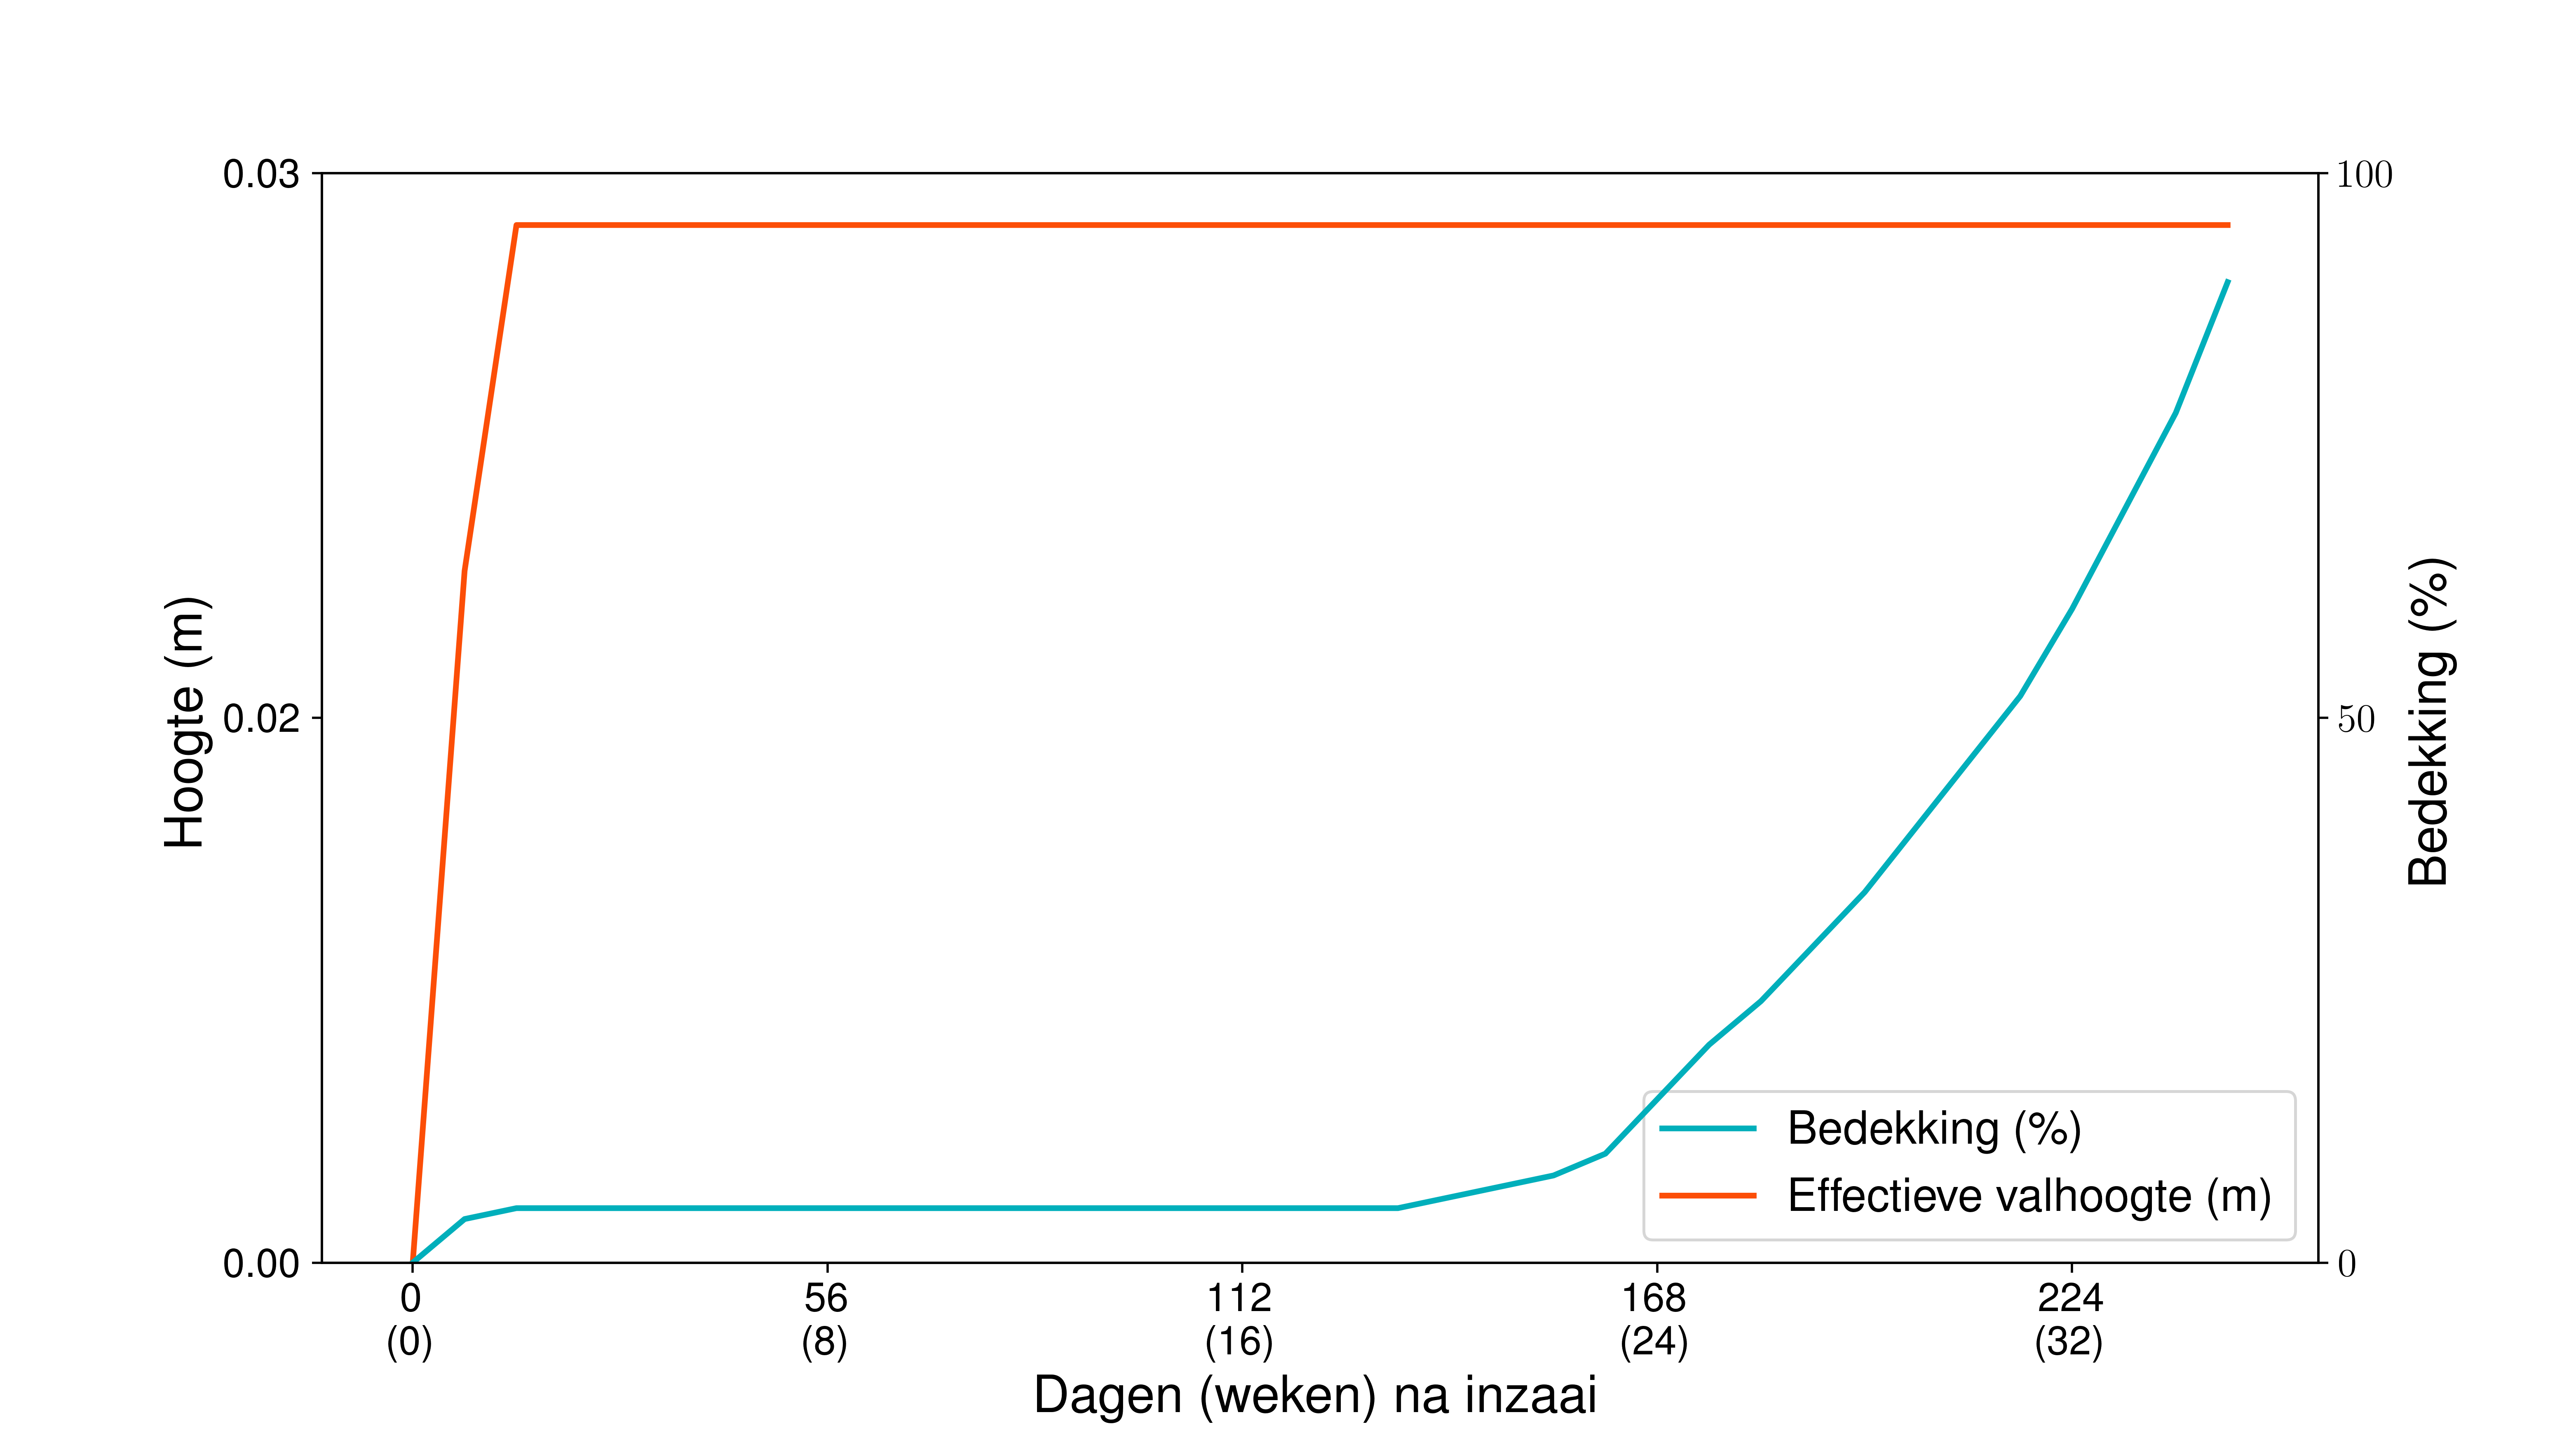
\includegraphics[width=12.5cm]{temp/5016.png} \end{figure} \end{center} 
  \textbf{Referenties:} Gabriels2003;KMI2003;RUSLE;ILVO2019 \vspace{0.10cm} \\ 
  \textbf{Opmerkingen?} geen \vspace{0.10cm} \\ 
 \newpage 
 \section{Eenjarige klaver (groep\_id 18)} 
 \textbf{Van toepassing op gewasnamen (en codes):} Eenjarige klaver (721) 
 \begin{multicols}{3} \begin{itemize} \item[$\square$] Meerjarig \item[$\square$] Groenbedekker \item[$\square$] Groente \end{itemize} \end{multicols} 
  \textbf{Zaaidatum (dd/mm)}: 15/09  \vspace{0.10cm} \\ 
  \textbf{Oogstdatum (dd/mm)}: 15/06  \vspace{0.10cm} \\ 
  \textbf{Oogstresten} \vspace{0.05cm} \\ 
  \tab Initi\"{e}le hoeveelheid (kg ha$^{-1}$): 2200.00 \vspace{0.05cm} \\ 
  \tab Afbraakcoefficient (-): 0.03 \vspace{0.05cm} \\ 
  \tab Bodembedekking (m$^2$ kg$^{-1}$): 4.18 \vspace{0.05cm} \\ 
  \tab Initieel percentage bedekking (\%): 100 \vspace{0.05cm} \\ 
  \tab Halfwaarde tijd (dagen): 10 \vspace{0.05cm} \\ 
  \textbf{Initi\"{e}le bodemruwheid (mm)}: 7.60 \vspace{0.05cm} \\ 
  \textbf{Gewasgroeicurve subgroep\_id 1018:} 
 \begin{center} \begin{figure}[H] 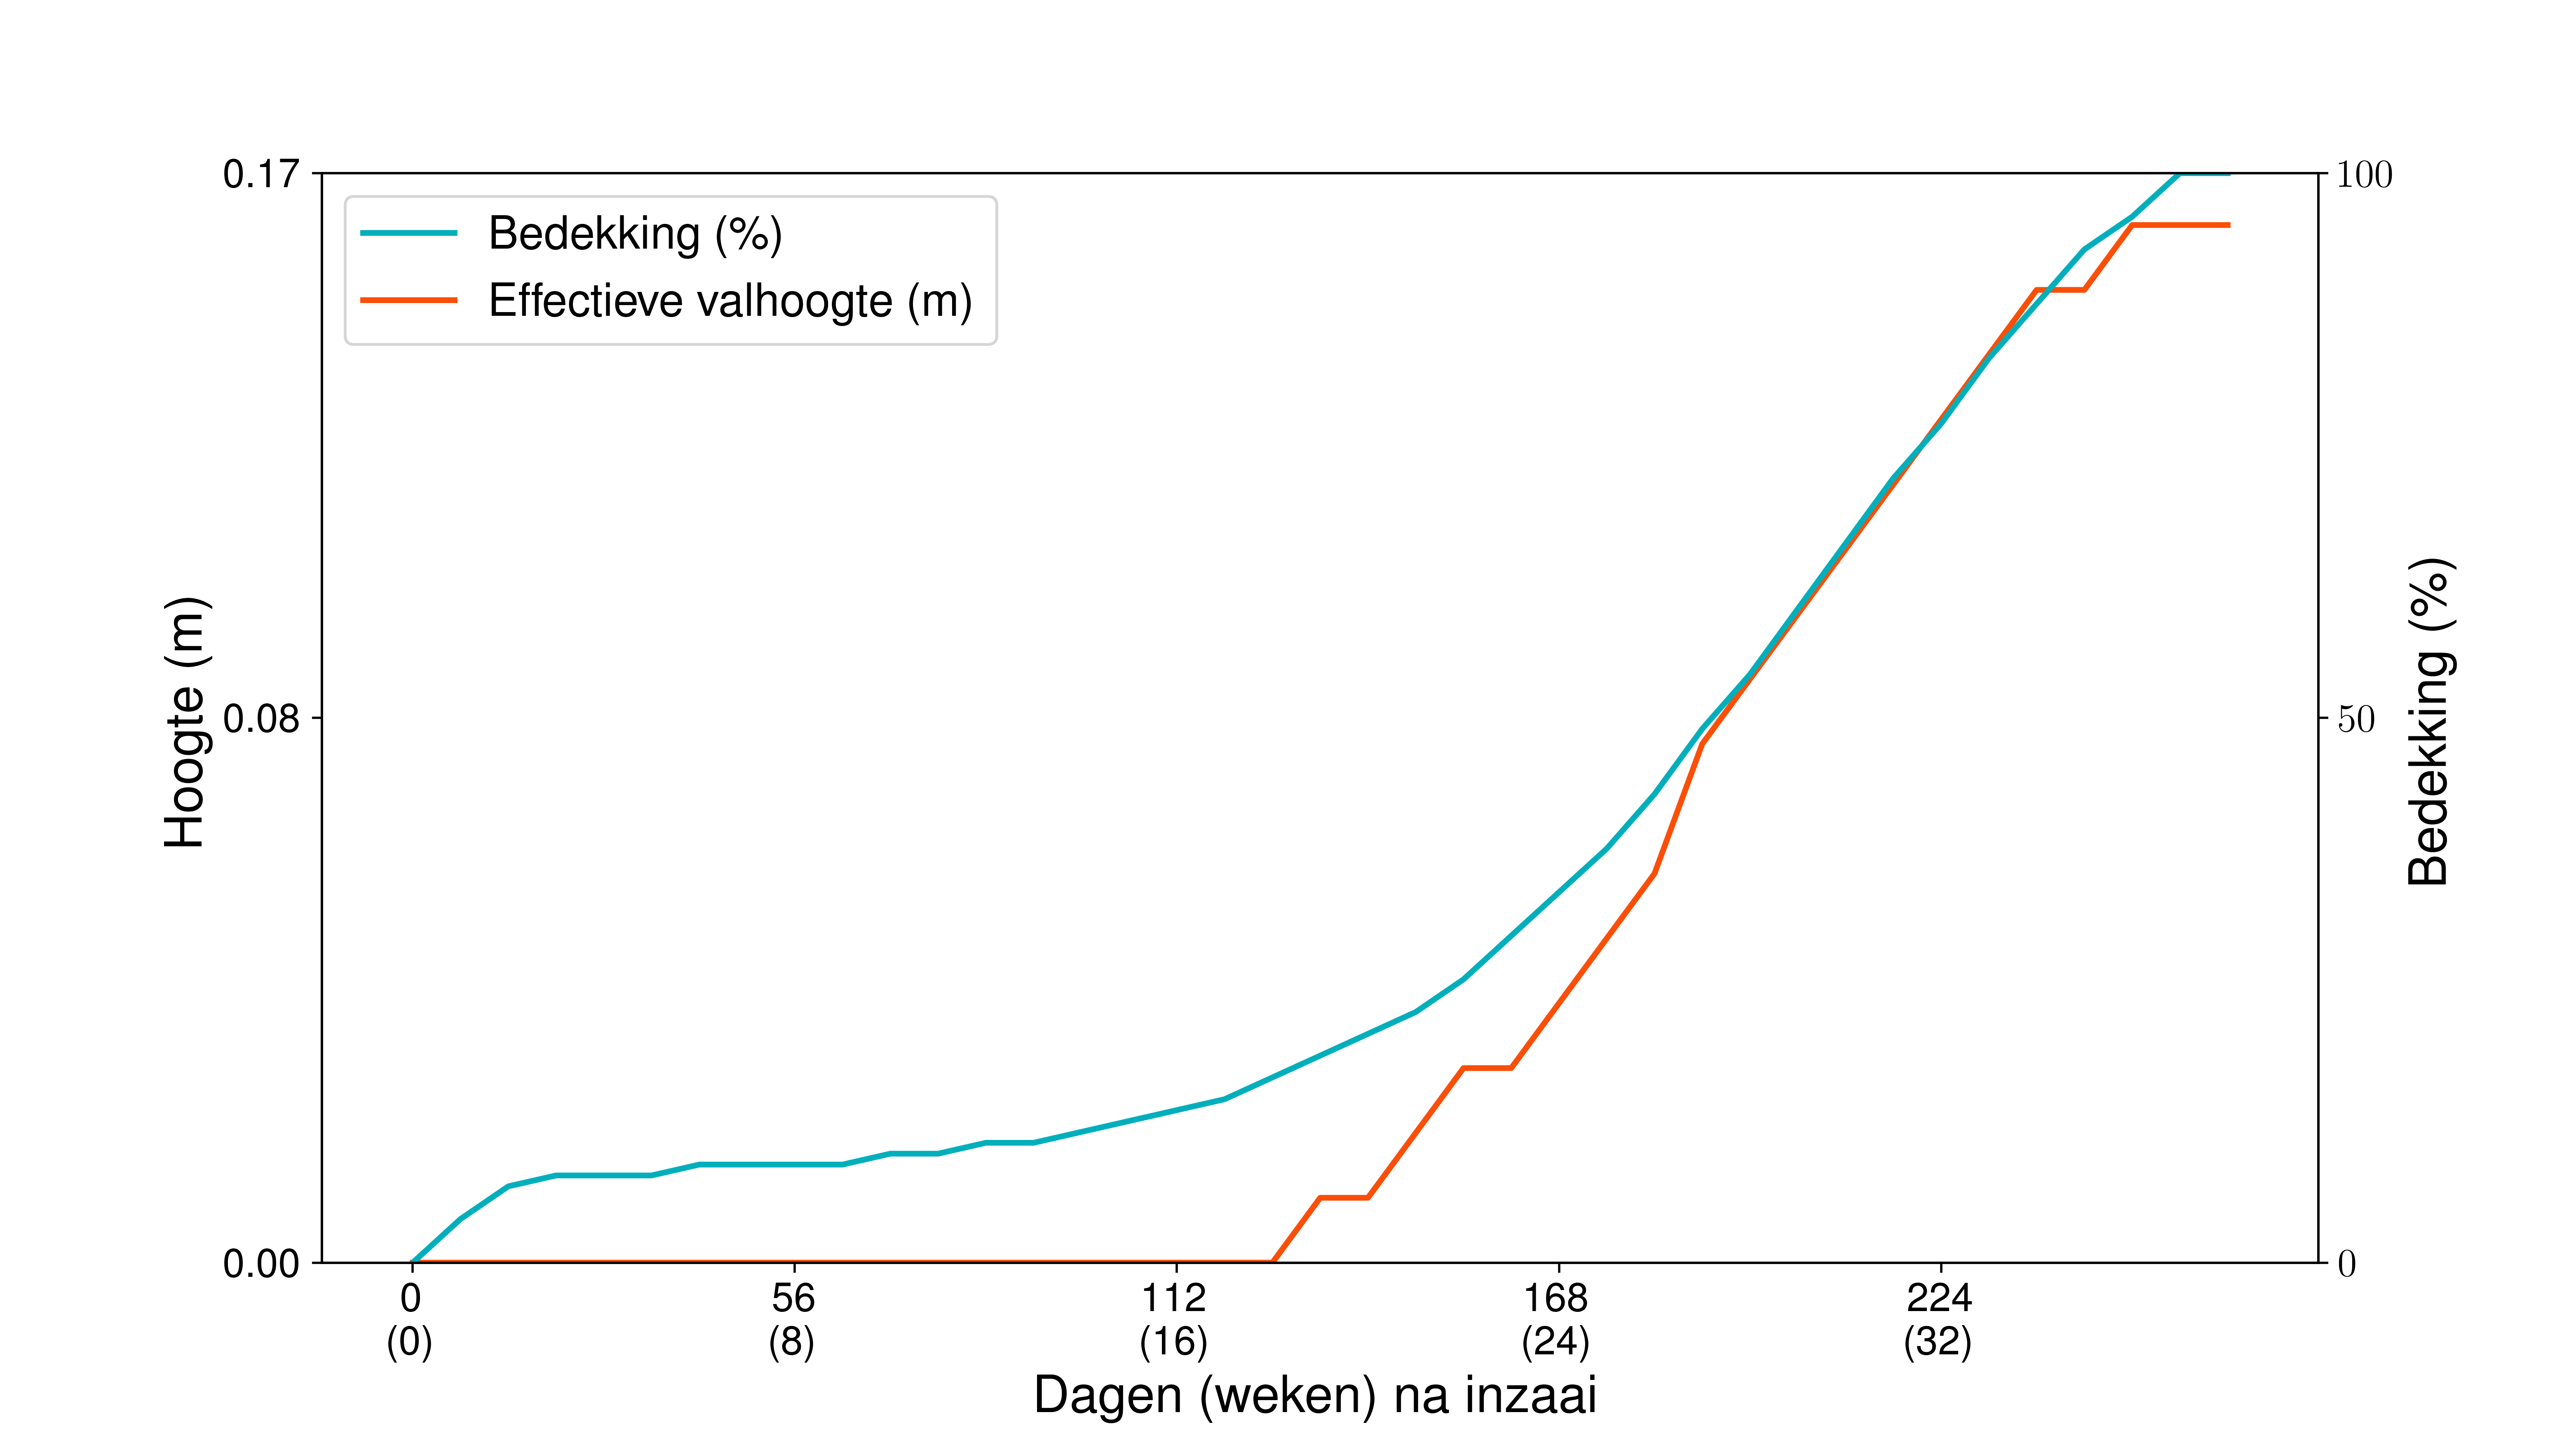
\includegraphics[width=12.5cm]{temp/1018.png} \end{figure} \end{center} 
  \textbf{Referenties:} ILVO2019;RUSLE \vspace{0.10cm} \\ 
  \textbf{Opmerkingen?} geen \vspace{0.10cm} \\ 
 \newpage 
 \section{Eenjarige luzerne (groep\_id 19)} 
 \textbf{Van toepassing op gewasnamen (en codes):} Eenjarige luzerne (731) 
 \begin{multicols}{3} \begin{itemize} \item[$\square$] Meerjarig \item[$\square$] Groenbedekker \item[$\square$] Groente \end{itemize} \end{multicols} 
  \textbf{Zaaidatum (dd/mm)}: 15/03  \vspace{0.10cm} \\ 
  \textbf{Oogstdatum (dd/mm)}: 15/09  \vspace{0.10cm} \\ 
  \textbf{Oogstresten} \vspace{0.05cm} \\ 
  \tab Initi\"{e}le hoeveelheid (kg ha$^{-1}$): 3000.00 \vspace{0.05cm} \\ 
  \tab Afbraakcoefficient (-): 0.02 \vspace{0.05cm} \\ 
  \tab Bodembedekking (m$^2$ kg$^{-1}$): 4.18 \vspace{0.05cm} \\ 
  \tab Initieel percentage bedekking (\%): 71 \vspace{0.05cm} \\ 
  \tab Halfwaarde tijd (dagen): 15 \vspace{0.05cm} \\ 
  \textbf{Initi\"{e}le bodemruwheid (mm)}: 7.60 \vspace{0.05cm} \\ 
  \textbf{Gewasgroeicurve subgroep\_id 1019:} 
 \begin{center} \begin{figure}[H] 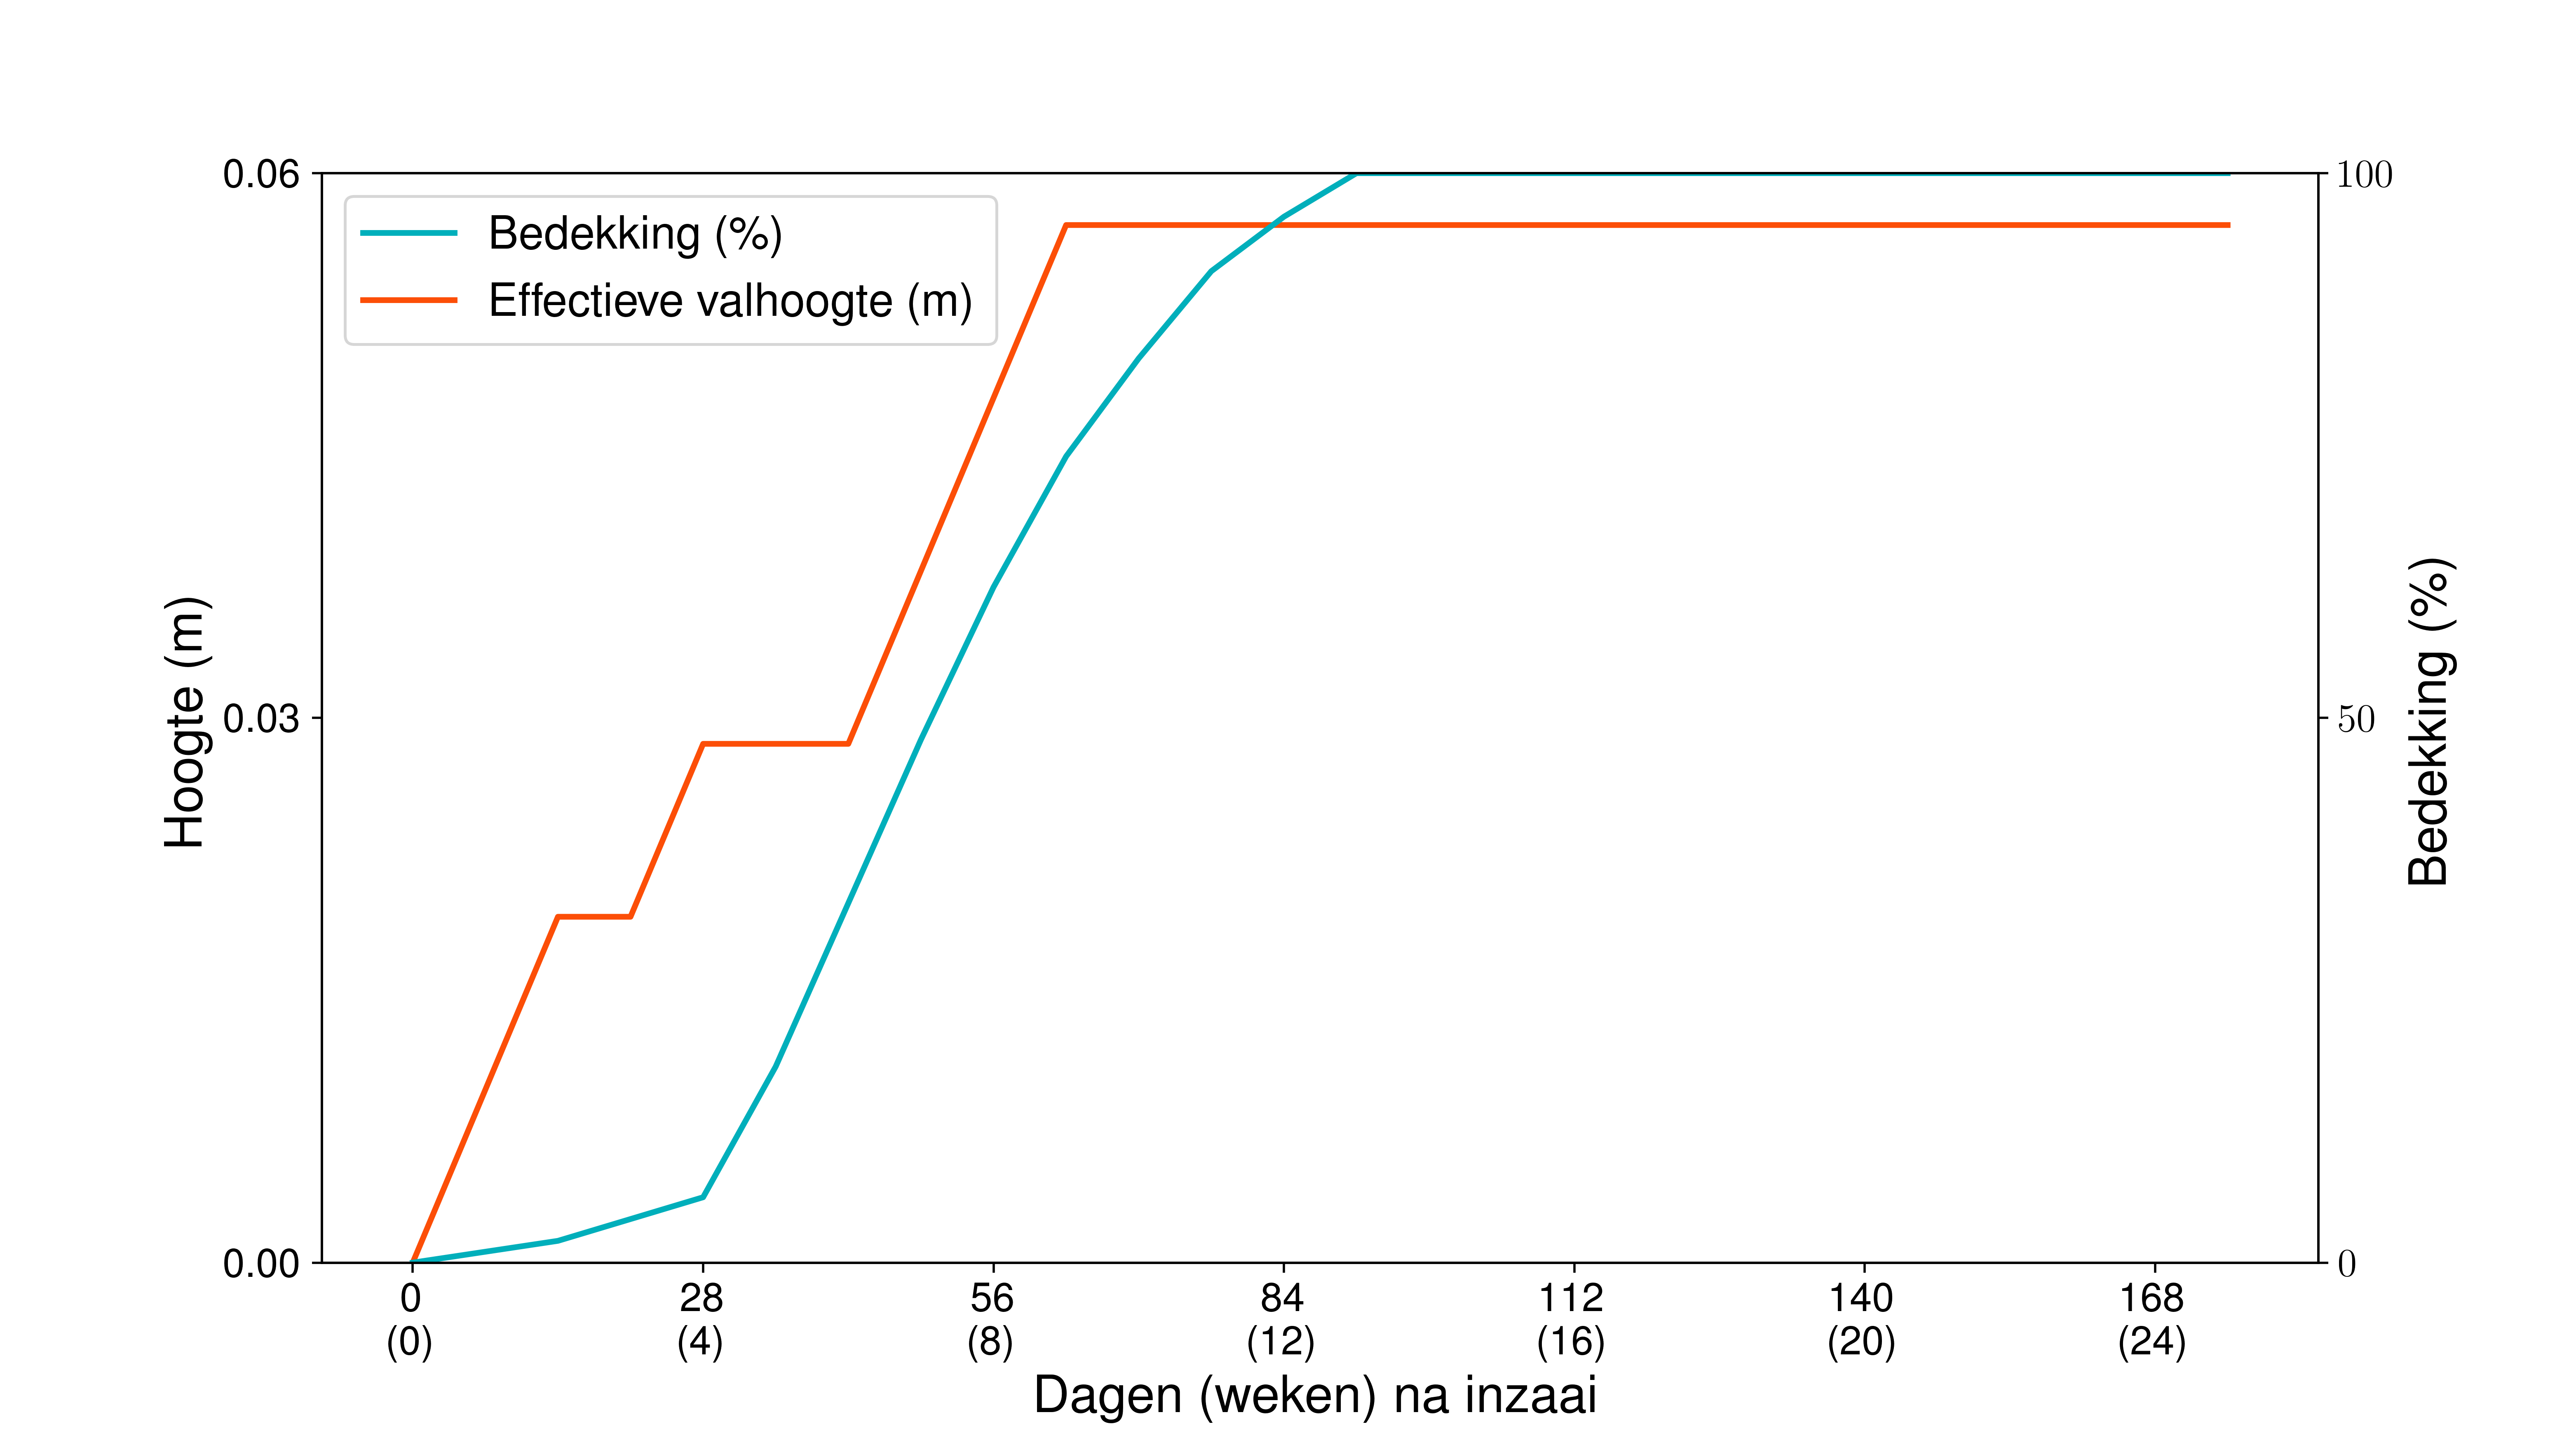
\includegraphics[width=12.5cm]{temp/1019.png} \end{figure} \end{center} 
  \textbf{Referenties:} ILVO2019;RUSLE \vspace{0.10cm} \\ 
  \textbf{Opmerkingen?} geen \vspace{0.10cm} \\ 
 \newpage 
 \section{Gele mosterd en bladrammanas (groep\_id 20)} 
 \textbf{Van toepassing op gewasnamen (en codes):} Gele mosterd (643) , Bladrammenas (656) , Andere vlinderbloemige groenbedekkers (648) , Mengsel met 1 of meer vlinderbloemige groenbedekkers (658) , Mengsel van niet-vlinderbloemige groenbedekkers (659) 
 \begin{multicols}{3} \begin{itemize} \item[$\square$] Meerjarig \item[$\boxtimes$] Groenbedekker \item[$\square$] Groente \end{itemize} \end{multicols} 
 \subsection{Hoofdteelt, voorteelt en nateelt (inzaaidatum=[0801,0915]) (subgroep\_id 1020)} 
  \textbf{Zaaidatum (dd/mm)}: 01/08  \vspace{0.10cm} \\ 
  \textbf{Oogstdatum (dd/mm)}: /9  \vspace{0.10cm} \\ 
  \textbf{Oogstresten} \vspace{0.05cm} \\ 
  \tab Initi\"{e}le hoeveelheid (kg ha$^{-1}$): 2000.00 \vspace{0.05cm} \\ 
  \tab Afbraakcoefficient (-): 0.05 \vspace{0.05cm} \\ 
  \tab Bodembedekking (m$^2$ kg$^{-1}$): 3.47 \vspace{0.05cm} \\ 
  \tab Initieel percentage bedekking (\%): 50 \vspace{0.05cm} \\ 
  \tab Halfwaarde tijd (dagen): 6 \vspace{0.05cm} \\ 
  \textbf{Initi\"{e}le bodemruwheid (mm)}: 7.60 \vspace{0.05cm} \\ 
  \textbf{Gewasgroeicurve subgroep\_id 1020:} 
 \begin{center} \begin{figure}[H] 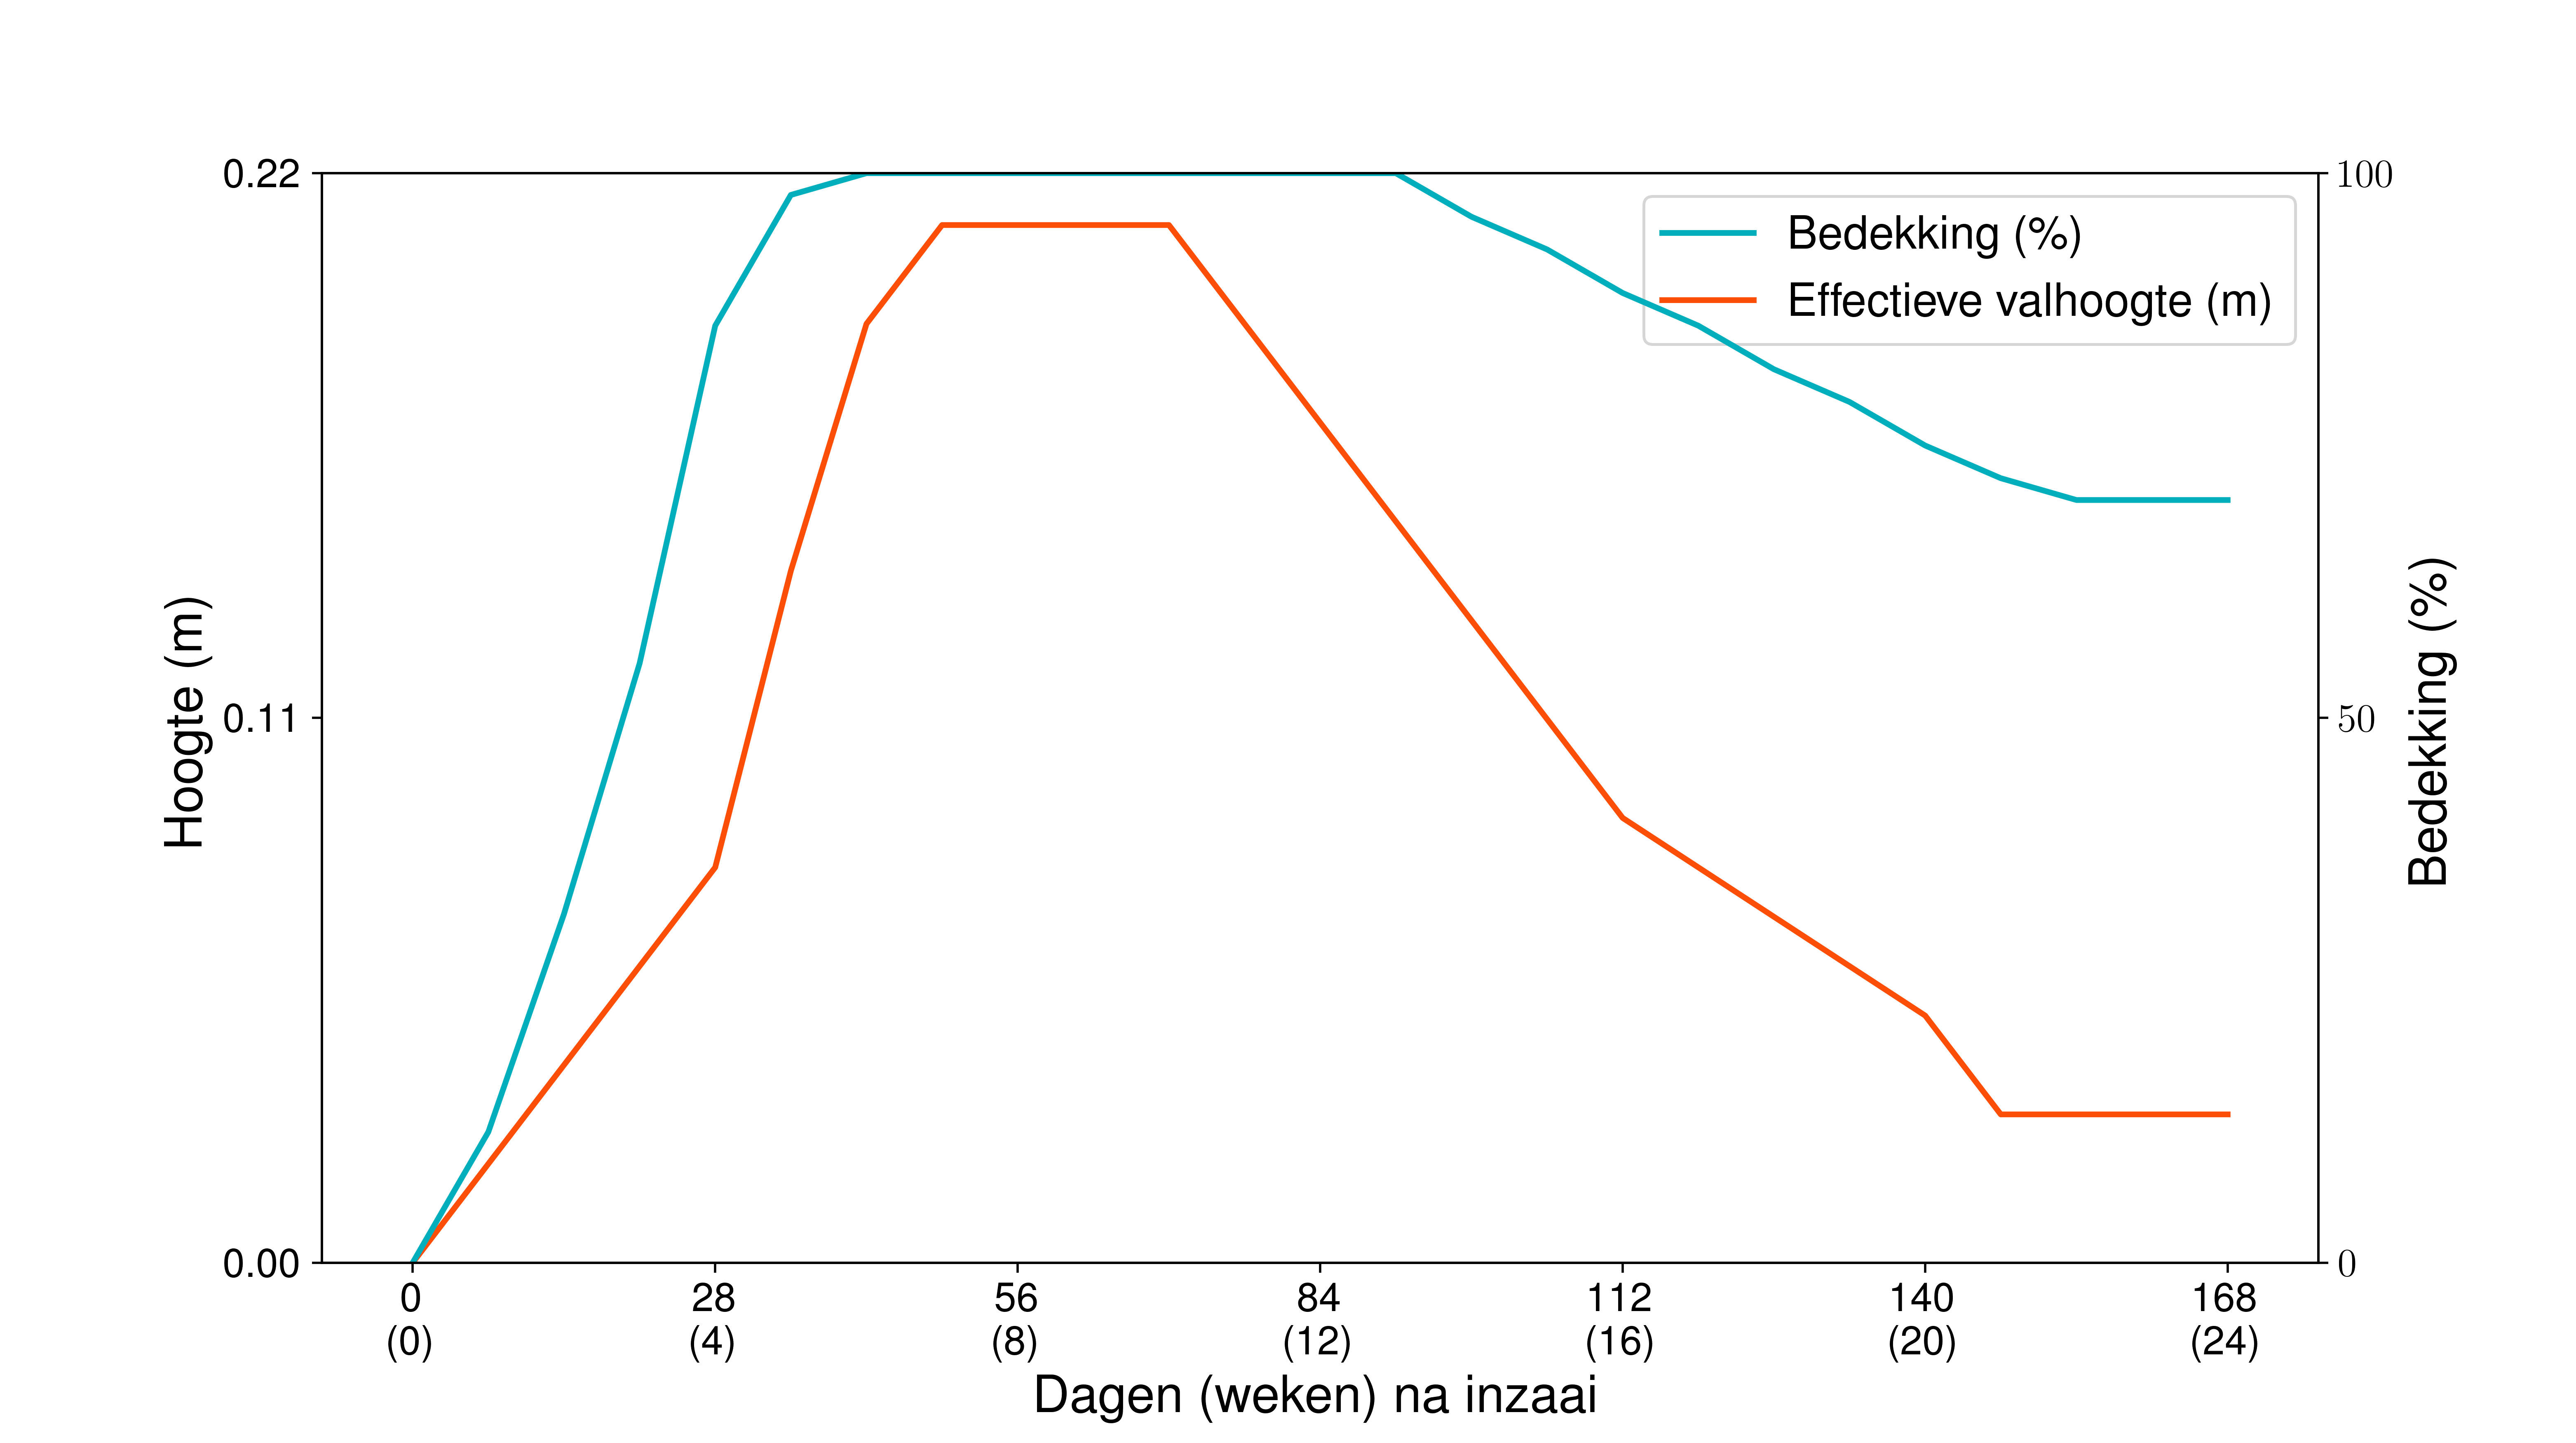
\includegraphics[width=12.5cm]{temp/1020.png} \end{figure} \end{center} 
  \textbf{Referenties:} KMI2003;RUSLE;ILVO2019 \vspace{0.10cm} \\ 
  \textbf{Opmerkingen?} geen \vspace{0.10cm} \\ 
 \newpage 
 \subsection{Hoofdteelt, voorteelt en nateelt (inzaaidatum=[0915,1029]) (subgroep\_id 2020)} 
  \textbf{Zaaidatum (dd/mm)}: 15/09  \vspace{0.10cm} \\ 
  \textbf{Oogstdatum (dd/mm)}: /9  \vspace{0.10cm} \\ 
  \textbf{Oogstresten} \vspace{0.05cm} \\ 
  \tab Initi\"{e}le hoeveelheid (kg ha$^{-1}$): 2000.00 \vspace{0.05cm} \\ 
  \tab Afbraakcoefficient (-): 0.05 \vspace{0.05cm} \\ 
  \tab Bodembedekking (m$^2$ kg$^{-1}$): 3.47 \vspace{0.05cm} \\ 
  \tab Initieel percentage bedekking (\%): 50 \vspace{0.05cm} \\ 
  \tab Halfwaarde tijd (dagen): 6 \vspace{0.05cm} \\ 
  \textbf{Initi\"{e}le bodemruwheid (mm)}: 7.60 \vspace{0.05cm} \\ 
  \textbf{Gewasgroeicurve subgroep\_id 2020:} 
 \begin{center} \begin{figure}[H] 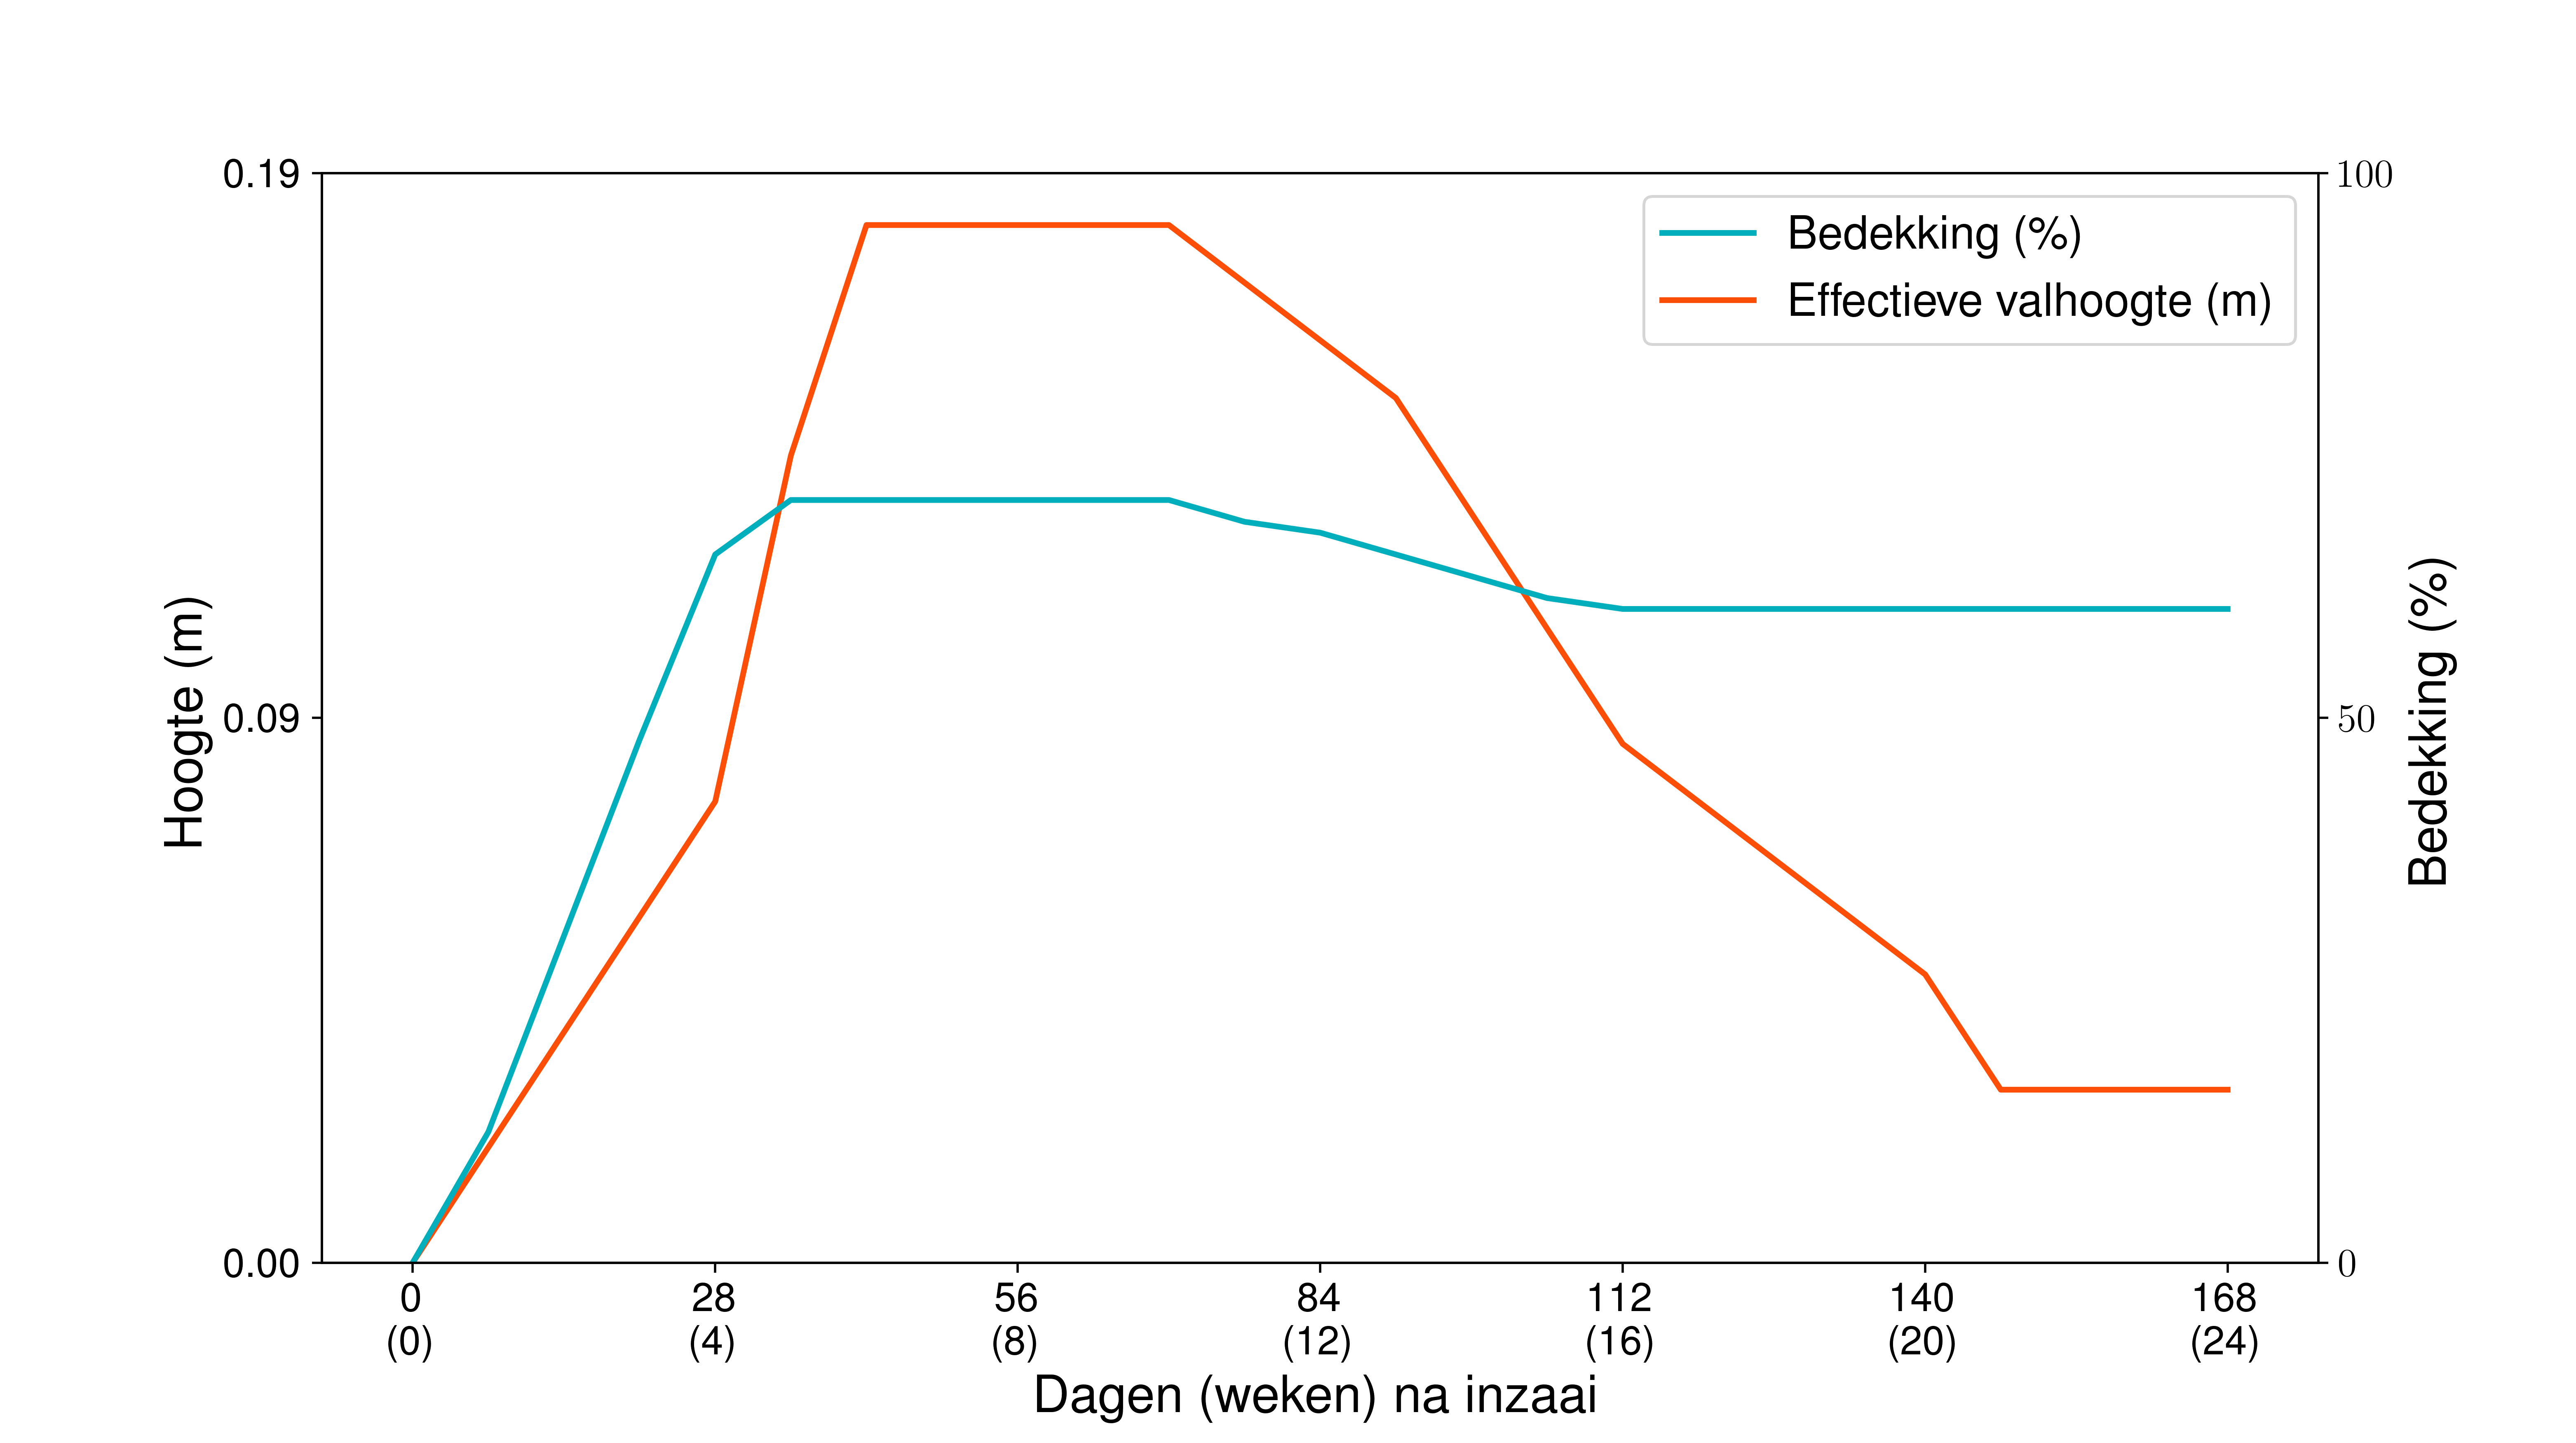
\includegraphics[width=12.5cm]{temp/2020.png} \end{figure} \end{center} 
  \textbf{Referenties:} KMI2003;RUSLE;ILVO2019 \vspace{0.10cm} \\ 
  \textbf{Opmerkingen?} geen \vspace{0.10cm} \\ 
 \newpage 
 \subsection{Hoofdteelt, voorteelt en nateelt (inzaaidatum=[1030,1231]) (subgroep\_id 3020)} 
  \textbf{Zaaidatum (dd/mm)}: 30/10  \vspace{0.10cm} \\ 
  \textbf{Oogstdatum (dd/mm)}: /9  \vspace{0.10cm} \\ 
  \textbf{Oogstresten} \vspace{0.05cm} \\ 
  \tab Initi\"{e}le hoeveelheid (kg ha$^{-1}$): 2000.00 \vspace{0.05cm} \\ 
  \tab Afbraakcoefficient (-): 0.05 \vspace{0.05cm} \\ 
  \tab Bodembedekking (m$^2$ kg$^{-1}$): 3.47 \vspace{0.05cm} \\ 
  \tab Initieel percentage bedekking (\%): 50 \vspace{0.05cm} \\ 
  \tab Halfwaarde tijd (dagen): 6 \vspace{0.05cm} \\ 
  \textbf{Initi\"{e}le bodemruwheid (mm)}: 7.60 \vspace{0.05cm} \\ 
  \textbf{Gewasgroeicurve subgroep\_id 3020:} 
 \begin{center} \begin{figure}[H] 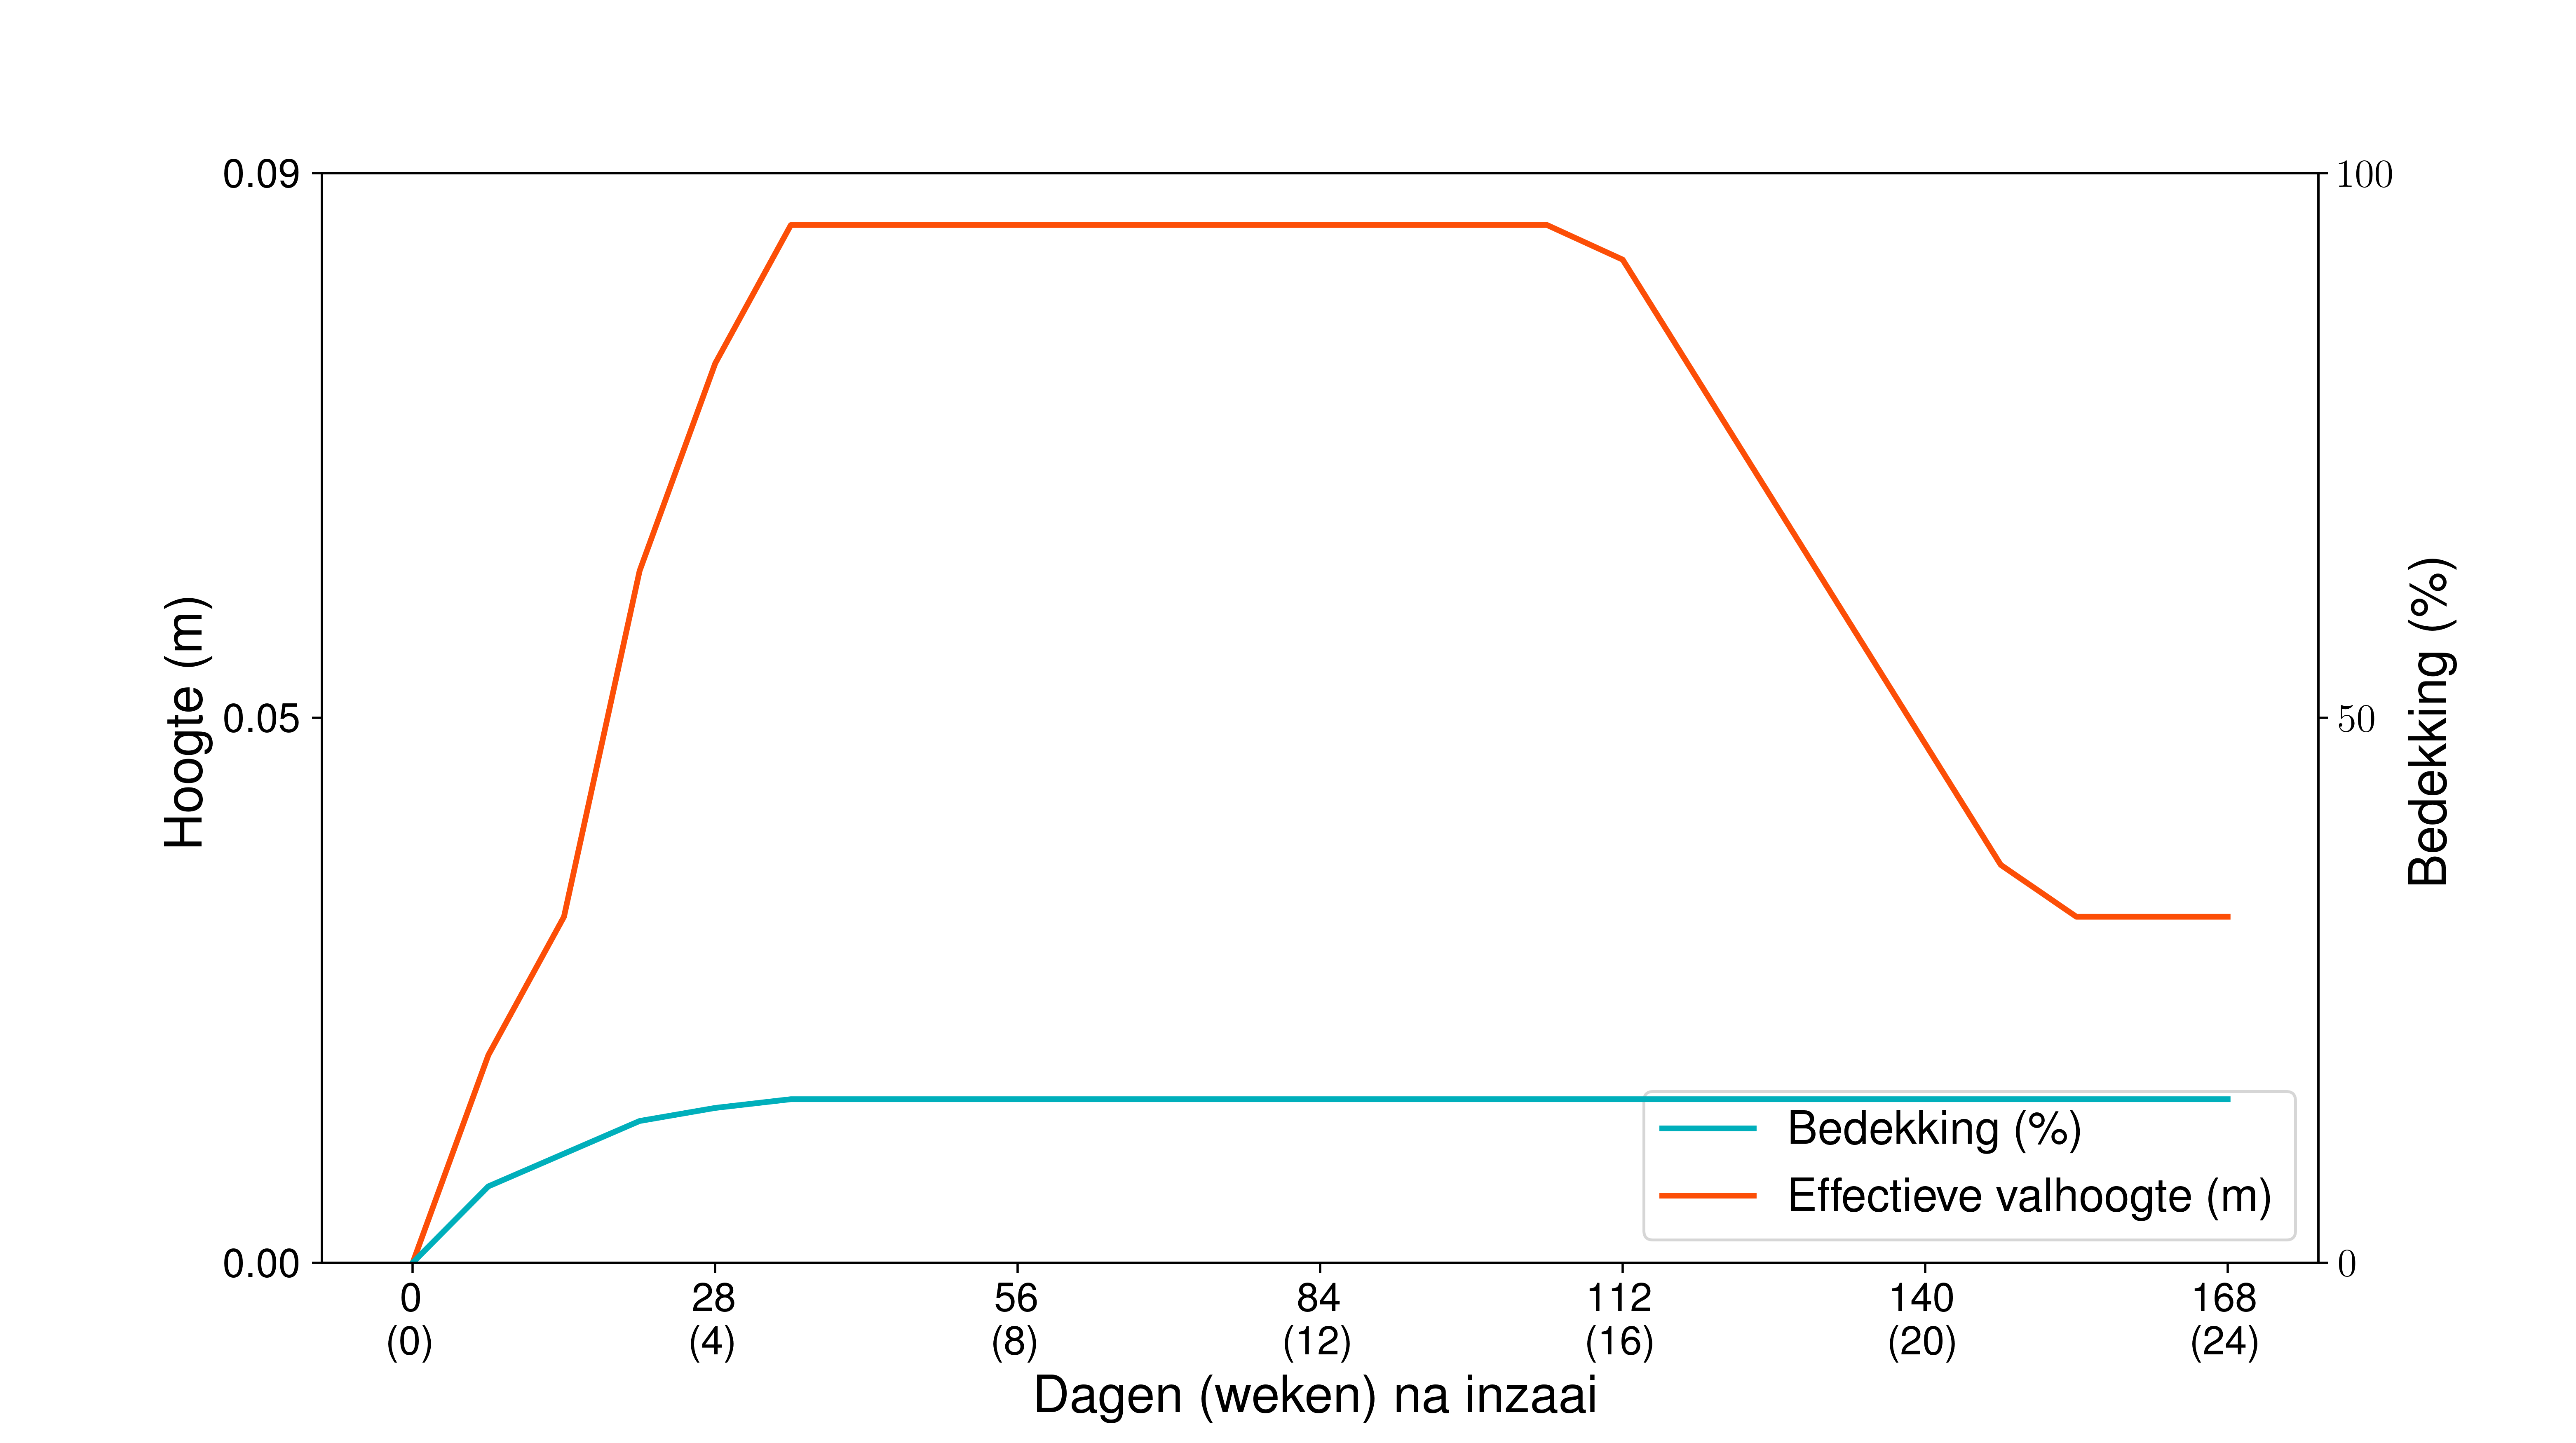
\includegraphics[width=12.5cm]{temp/3020.png} \end{figure} \end{center} 
  \textbf{Referenties:} KMI2003;RUSLE;ILVO2019 \vspace{0.10cm} \\ 
  \textbf{Opmerkingen?} geen \vspace{0.10cm} \\ 
 \newpage 
 \section{Facelia (groep\_id 21)} 
 \textbf{Van toepassing op gewasnamen (en codes):} Facelia (645) 
 \begin{multicols}{3} \begin{itemize} \item[$\square$] Meerjarig \item[$\boxtimes$] Groenbedekker \item[$\square$] Groente \end{itemize} \end{multicols} 
 \subsection{Hoofdteelt, voorteelt en nateelt (inzaaidatum=[0801,0814]) (subgroep\_id 1020)} 
  \textbf{Zaaidatum (dd/mm)}: 01/08  \vspace{0.10cm} \\ 
  \textbf{Oogstdatum (dd/mm)}: /9  \vspace{0.10cm} \\ 
  \textbf{Oogstresten} \vspace{0.05cm} \\ 
  \tab Initi\"{e}le hoeveelheid (kg ha$^{-1}$): 2000.00 \vspace{0.05cm} \\ 
  \tab Afbraakcoefficient (-): 0.05 \vspace{0.05cm} \\ 
  \tab Bodembedekking (m$^2$ kg$^{-1}$): 3.47 \vspace{0.05cm} \\ 
  \tab Initieel percentage bedekking (\%): 50 \vspace{0.05cm} \\ 
  \tab Halfwaarde tijd (dagen): 6 \vspace{0.05cm} \\ 
  \textbf{Initi\"{e}le bodemruwheid (mm)}: 7.60 \vspace{0.05cm} \\ 
  \textbf{Gewasgroeicurve subgroep\_id 1020:} 
 \begin{center} \begin{figure}[H] 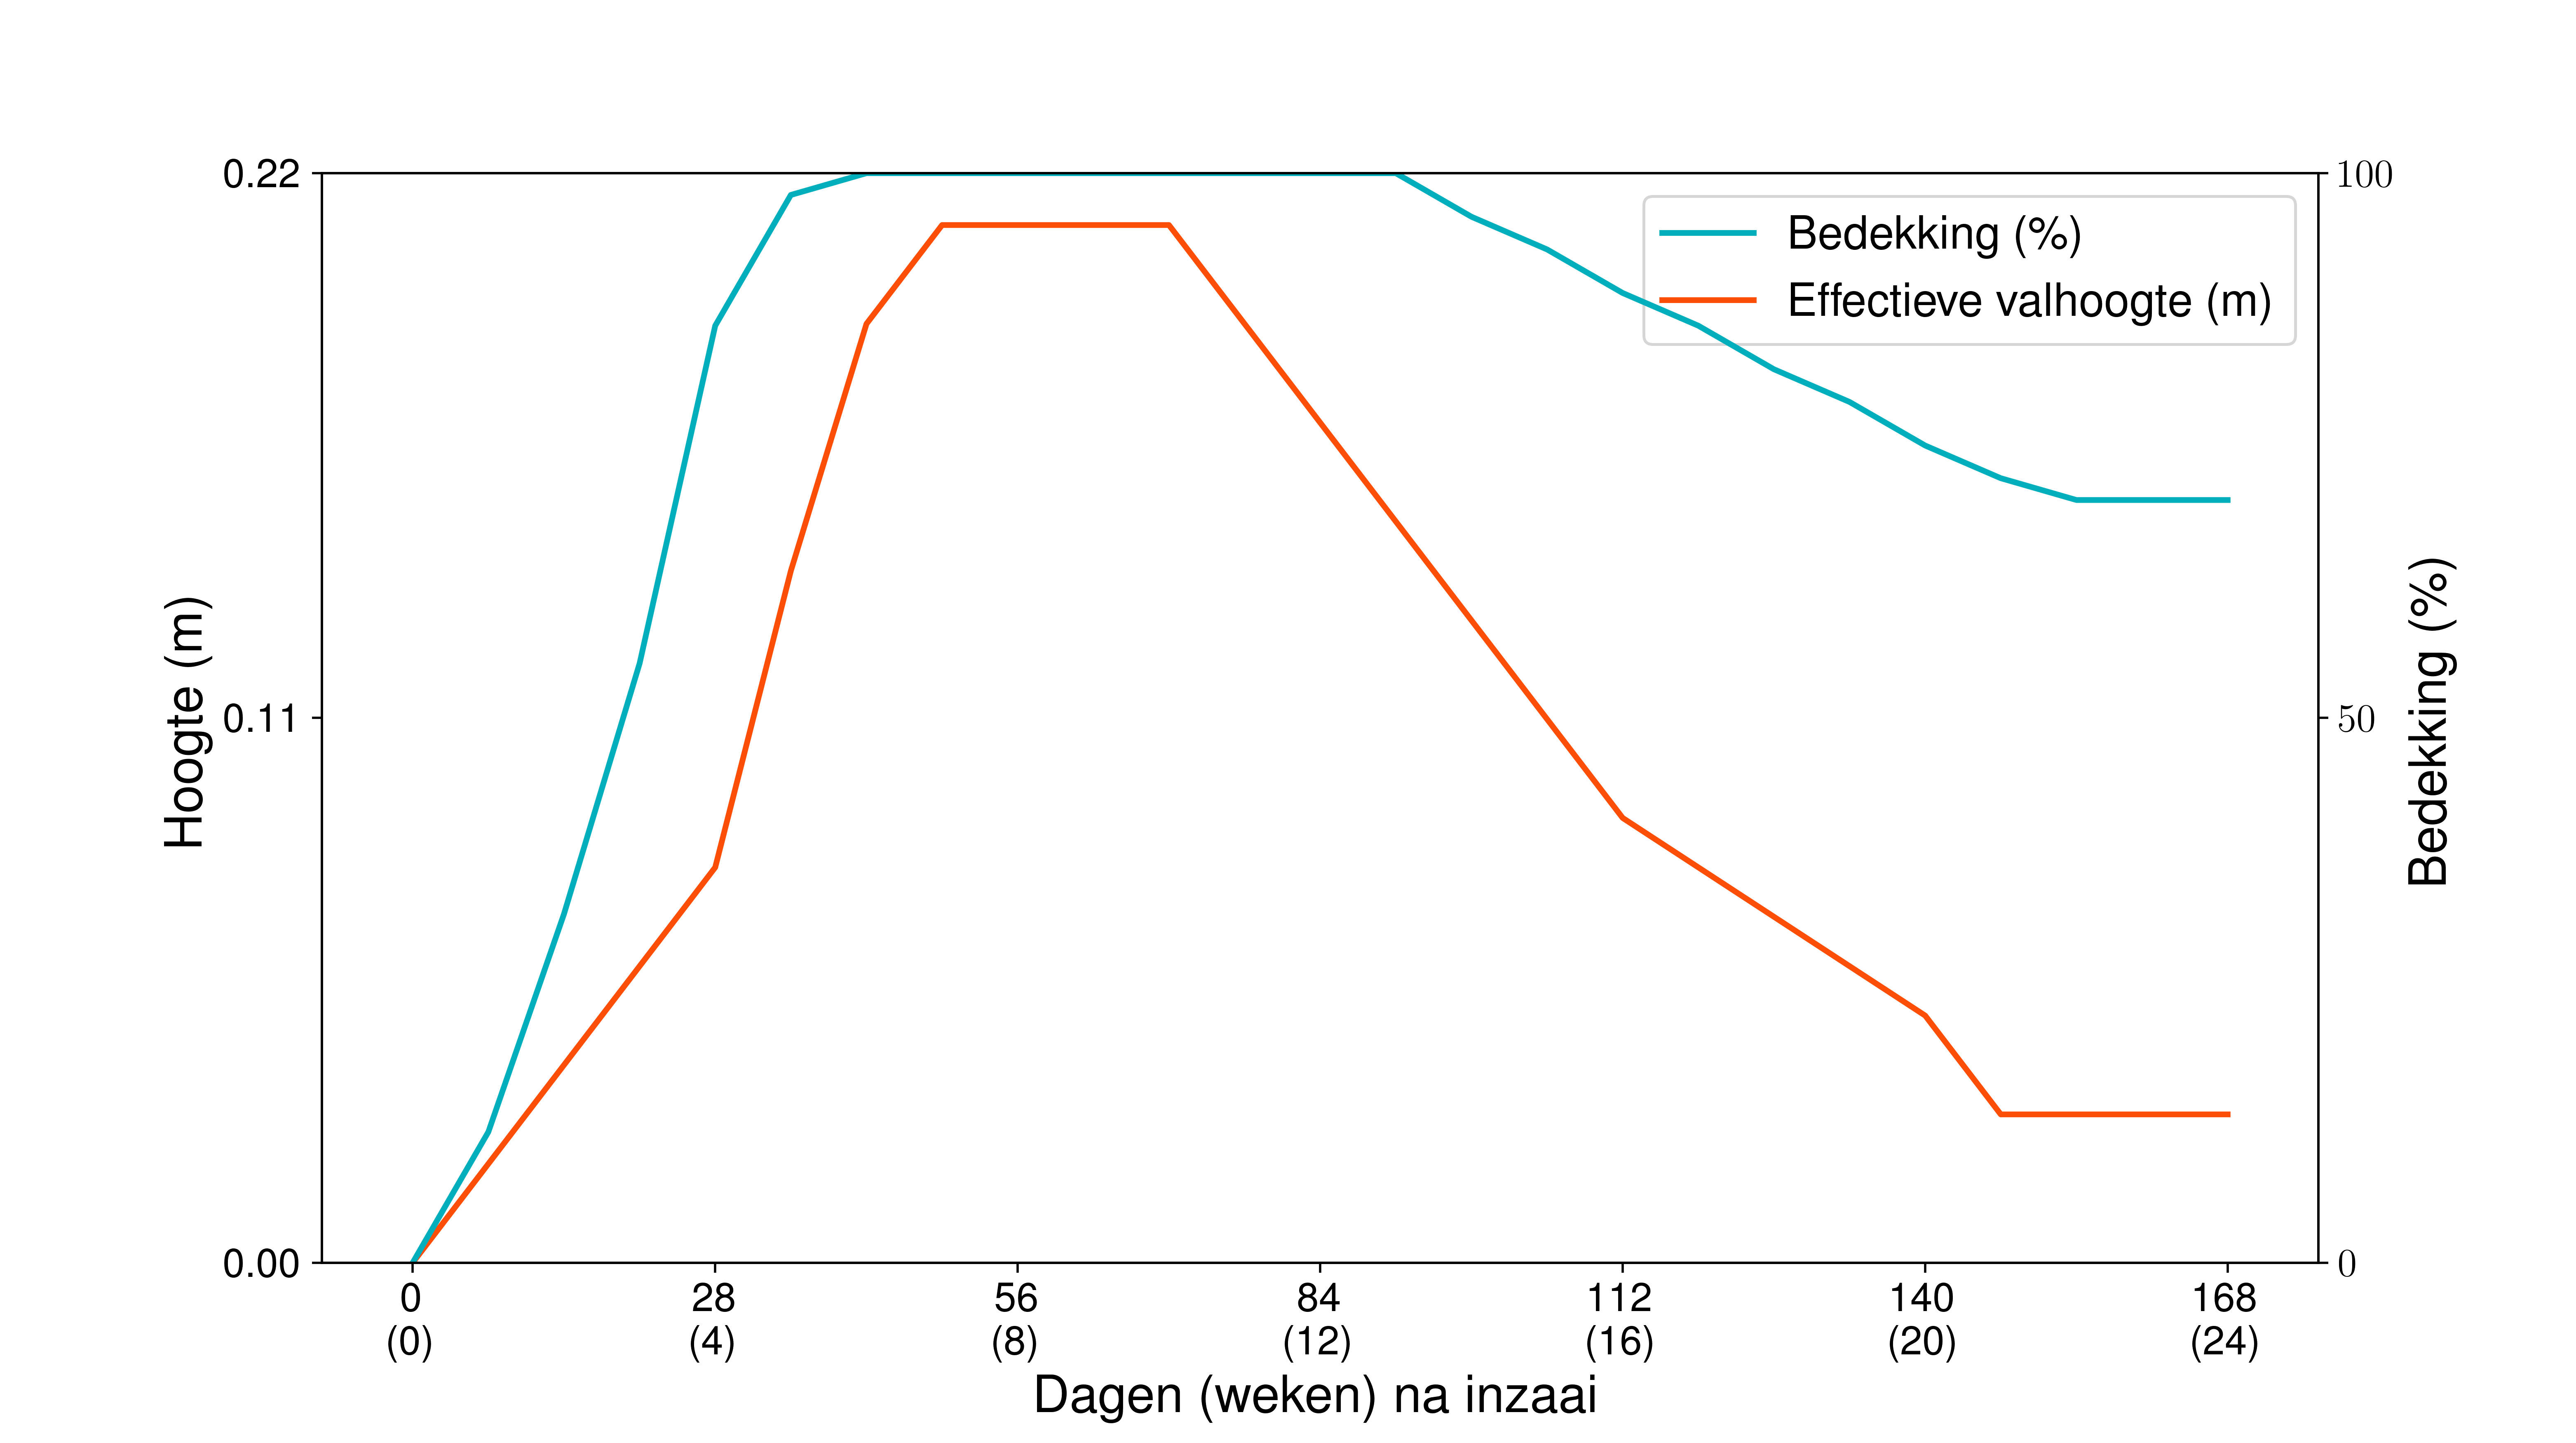
\includegraphics[width=12.5cm]{temp/1020.png} \end{figure} \end{center} 
  \textbf{Referenties:} KMI2003;RUSLE;ILVO2019 \vspace{0.10cm} \\ 
  \textbf{Opmerkingen?} geen \vspace{0.10cm} \\ 
 \newpage 
 \subsection{Hoofdteelt, voorteelt en nateelt (inzaaidatum=[0815,1231]) (subgroep\_id 2020)} 
  \textbf{Zaaidatum (dd/mm)}: 15/08  \vspace{0.10cm} \\ 
  \textbf{Oogstdatum (dd/mm)}: /9  \vspace{0.10cm} \\ 
  \textbf{Oogstresten} \vspace{0.05cm} \\ 
  \tab Initi\"{e}le hoeveelheid (kg ha$^{-1}$): 2000.00 \vspace{0.05cm} \\ 
  \tab Afbraakcoefficient (-): 0.05 \vspace{0.05cm} \\ 
  \tab Bodembedekking (m$^2$ kg$^{-1}$): 3.47 \vspace{0.05cm} \\ 
  \tab Initieel percentage bedekking (\%): 50 \vspace{0.05cm} \\ 
  \tab Halfwaarde tijd (dagen): 6 \vspace{0.05cm} \\ 
  \textbf{Initi\"{e}le bodemruwheid (mm)}: 7.60 \vspace{0.05cm} \\ 
  \textbf{Gewasgroeicurve subgroep\_id 2020:} 
 \begin{center} \begin{figure}[H] 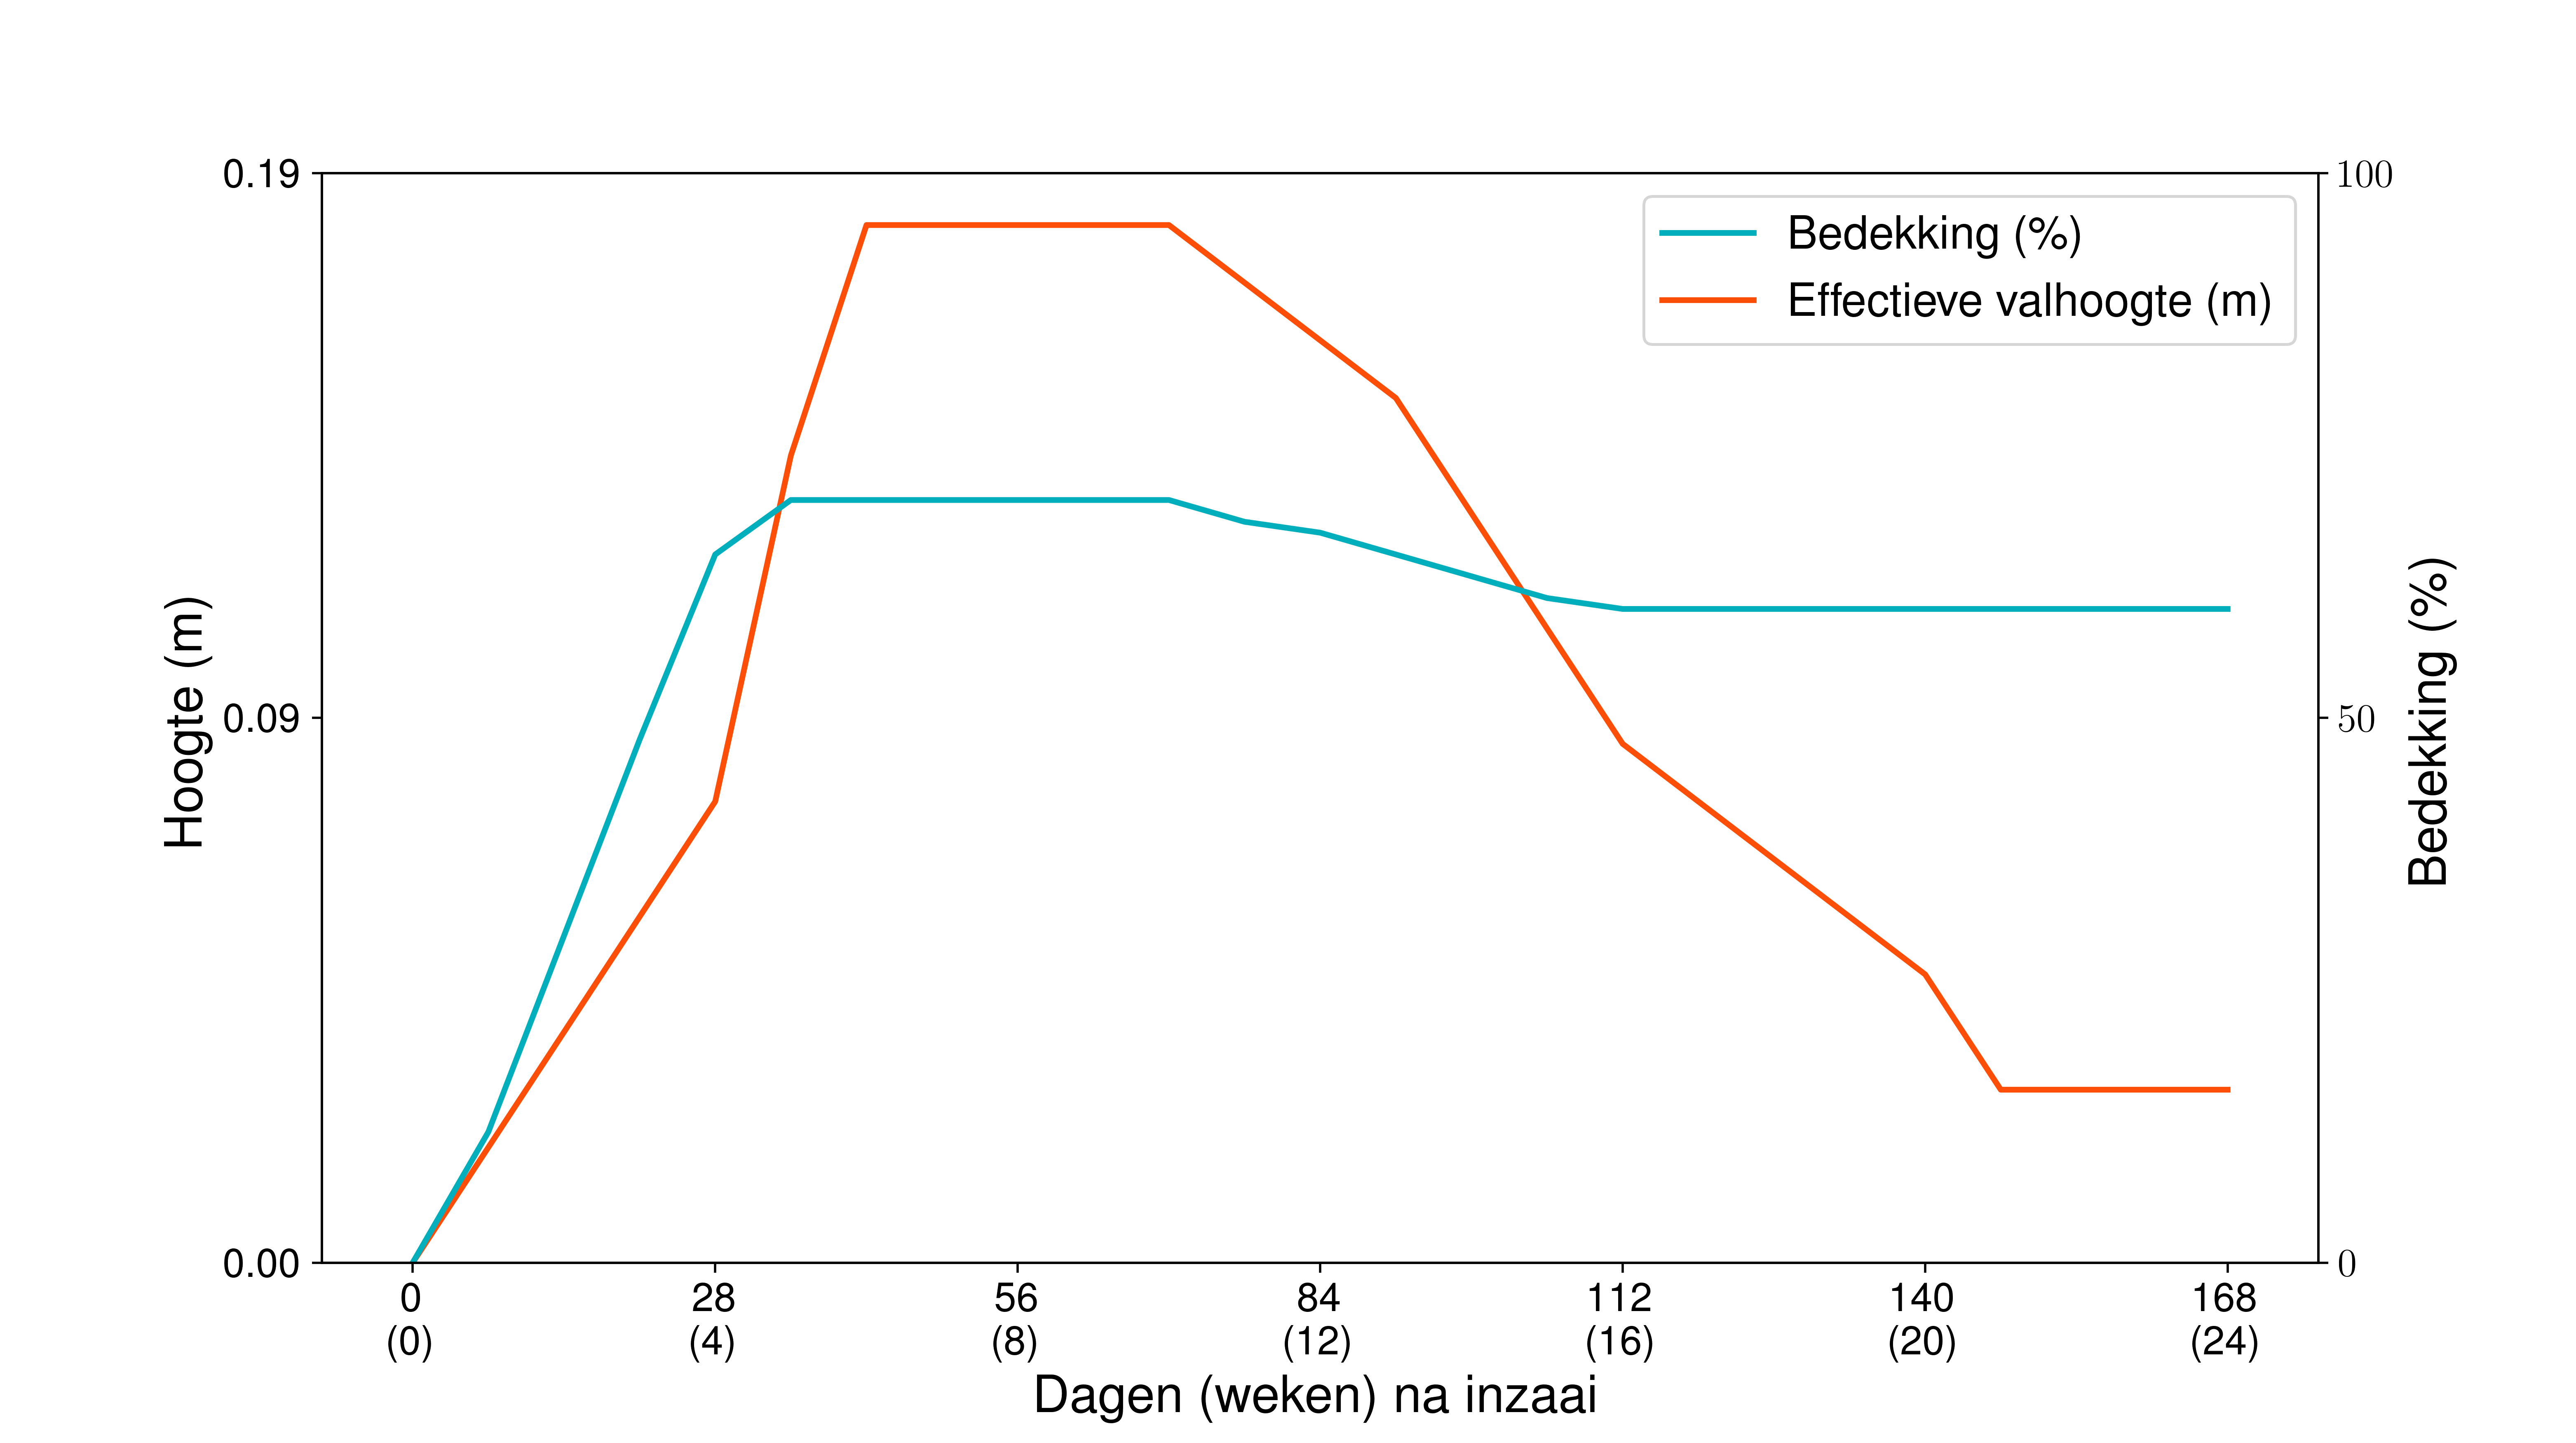
\includegraphics[width=12.5cm]{temp/2020.png} \end{figure} \end{center} 
  \textbf{Referenties:} KMI2003;RUSLE;ILVO2019 \vspace{0.10cm} \\ 
  \textbf{Opmerkingen?} geen \vspace{0.10cm} \\ 
 \newpage 
 \section{Ajuinen (groep\_id 25)} 
 \textbf{Van toepassing op gewasnamen (en codes):} Ajuinen (vroege) - industrie (8563) , Ajuinen (vroege) - vers (9563) 
 \begin{multicols}{3} \begin{itemize} \item[$\square$] Meerjarig \item[$\square$] Groenbedekker \item[$\boxtimes$] Groente \end{itemize} \end{multicols} 
  \textbf{Zaaidatum (dd/mm)}: 15/03  \vspace{0.10cm} \\ 
  \textbf{Oogstdatum (dd/mm)}: 15/08  \vspace{0.10cm} \\ 
  \textbf{Oogstresten} \vspace{0.05cm} \\ 
  \tab Initi\"{e}le hoeveelheid (kg ha$^{-1}$): 0.00 \vspace{0.05cm} \\ 
  \tab Afbraakcoefficient (-): 0.00 \vspace{0.05cm} \\ 
  \tab Bodembedekking (m$^2$ kg$^{-1}$): 0.00 \vspace{0.05cm} \\ 
  \tab Initieel percentage bedekking (\%): 0 \vspace{0.05cm} \\ 
  \tab Halfwaarde tijd (dagen): 0 \vspace{0.05cm} \\ 
  \textbf{Initi\"{e}le bodemruwheid (mm)}: 6.10 \vspace{0.05cm} \\ 
  \textbf{Gewasgroeicurve subgroep\_id 1025:} 
 \begin{center} \begin{figure}[H] 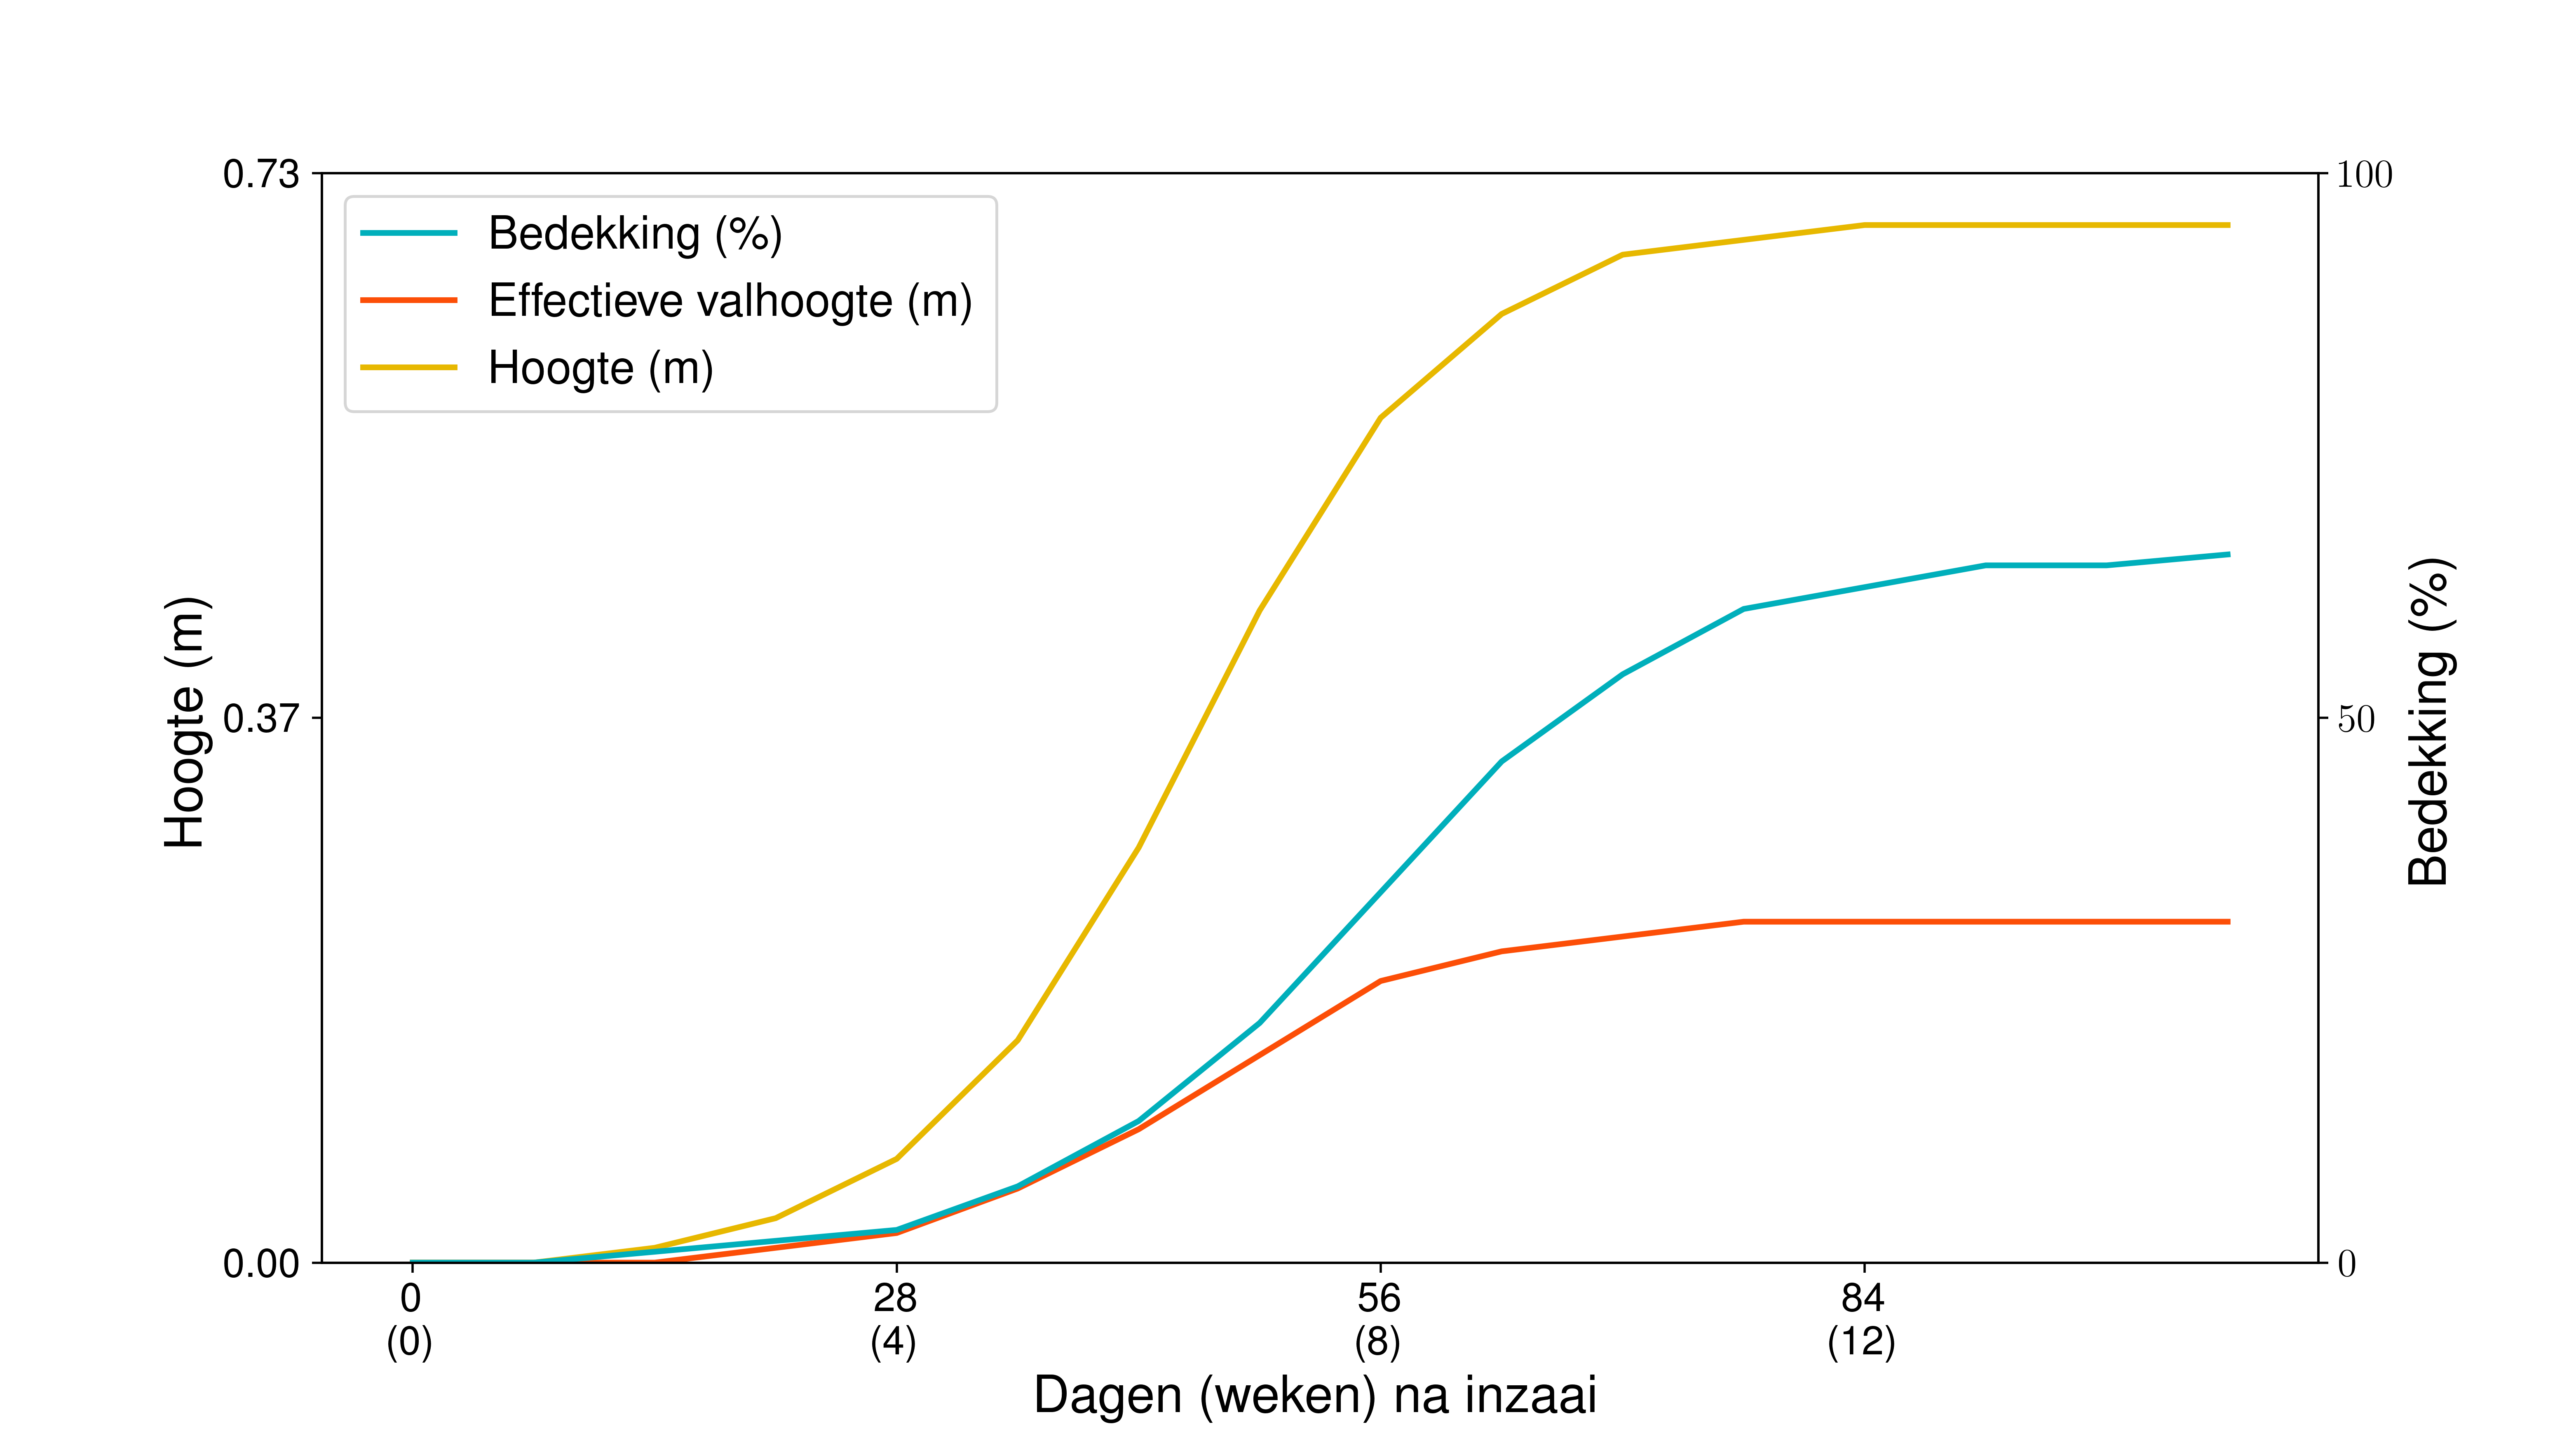
\includegraphics[width=12.5cm]{temp/1025.png} \end{figure} \end{center} 
  \textbf{Referenties:} ILVO2019.RUSLE \vspace{0.10cm} \\ 
  \textbf{Opmerkingen?} geen \vspace{0.10cm} \\ 
 \newpage 
 \section{Ajuinen (niet vroege) (groep\_id 26)} 
 \textbf{Van toepassing op gewasnamen (en codes):} Ajuinen (niet-vroege) - industrie (8514) , Ajuinen (niet vroege) - vers (9514) 
 \begin{multicols}{3} \begin{itemize} \item[$\square$] Meerjarig \item[$\square$] Groenbedekker \item[$\boxtimes$] Groente \end{itemize} \end{multicols} 
  \textbf{Zaaidatum (dd/mm)}: 01/04  \vspace{0.10cm} \\ 
  \textbf{Oogstdatum (dd/mm)}: 15/09  \vspace{0.10cm} \\ 
  \textbf{Oogstresten} \vspace{0.05cm} \\ 
  \tab Initi\"{e}le hoeveelheid (kg ha$^{-1}$): 0.00 \vspace{0.05cm} \\ 
  \tab Afbraakcoefficient (-): 0.00 \vspace{0.05cm} \\ 
  \tab Bodembedekking (m$^2$ kg$^{-1}$): 0.00 \vspace{0.05cm} \\ 
  \tab Initieel percentage bedekking (\%): 0 \vspace{0.05cm} \\ 
  \tab Halfwaarde tijd (dagen): 0 \vspace{0.05cm} \\ 
  \textbf{Initi\"{e}le bodemruwheid (mm)}: 6.10 \vspace{0.05cm} \\ 
  \textbf{Gewasgroeicurve subgroep\_id 1025:} 
 \begin{center} \begin{figure}[H] 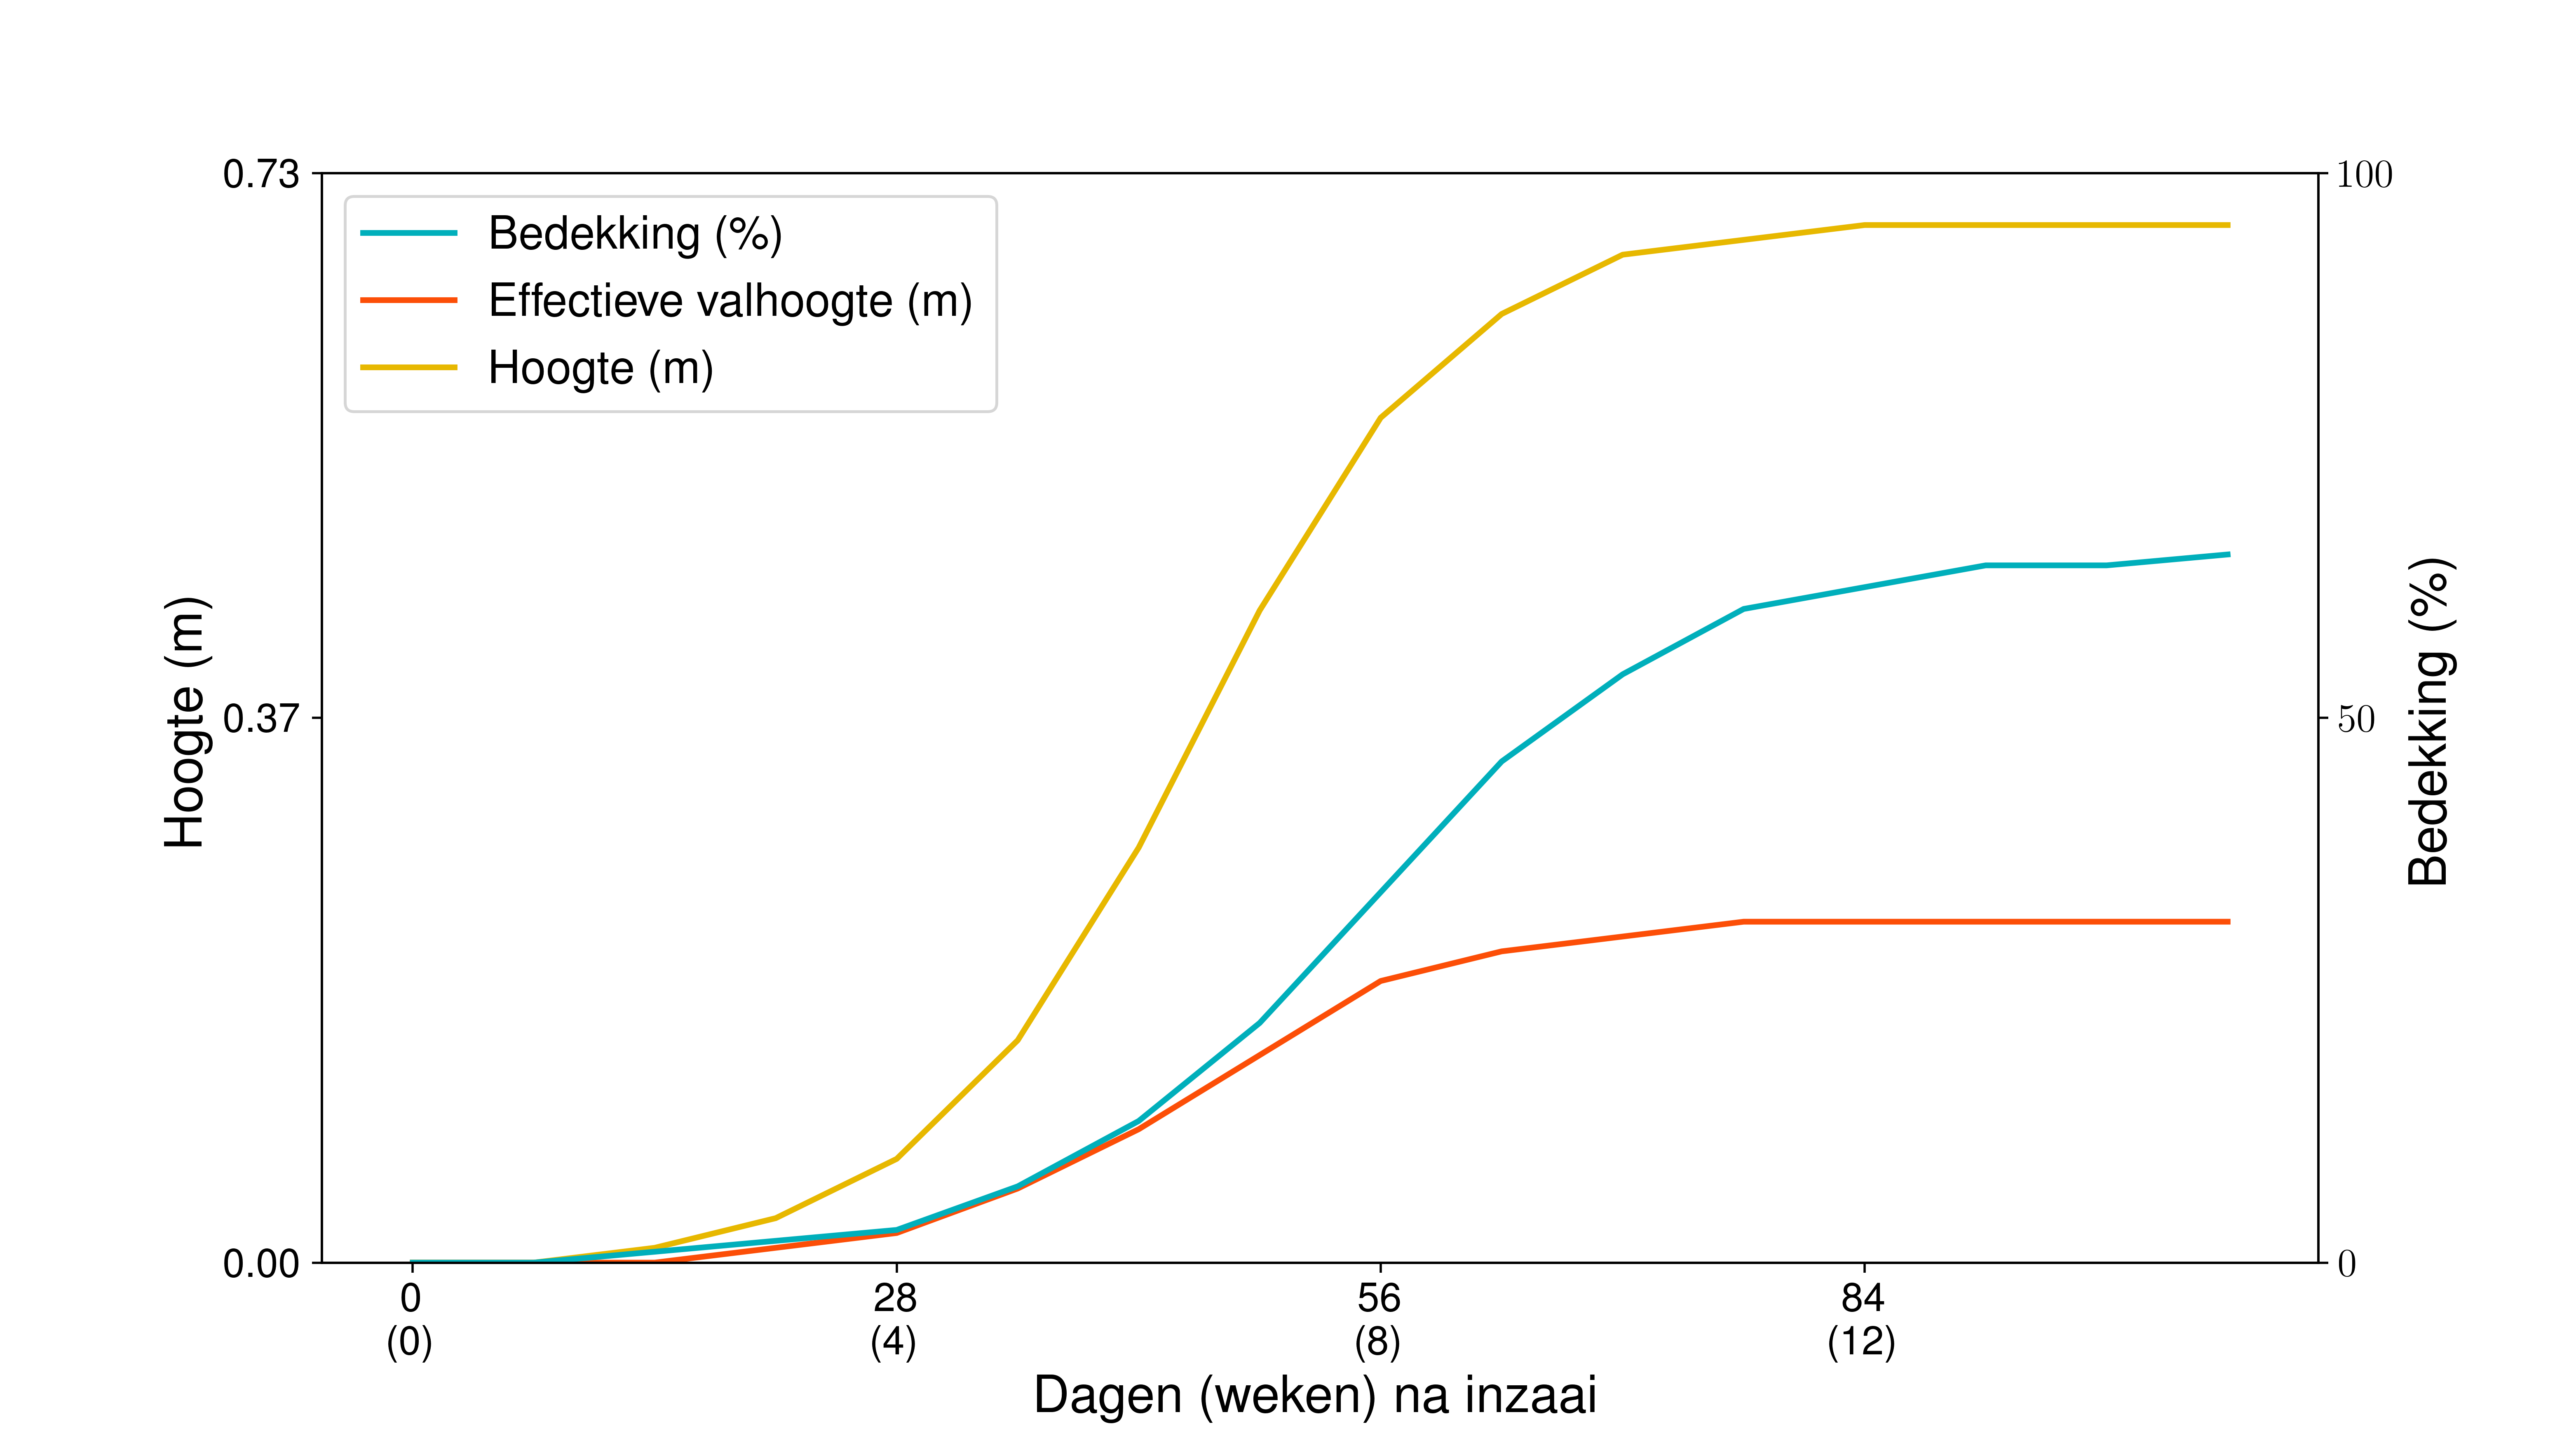
\includegraphics[width=12.5cm]{temp/1025.png} \end{figure} \end{center} 
  \textbf{Referenties:} ILVO2019.RUSLE \vspace{0.10cm} \\ 
  \textbf{Opmerkingen?} geen \vspace{0.10cm} \\ 
 \newpage 
 \section{Wortel (vroege) - industrie (groep\_id 27)} 
 \textbf{Van toepassing op gewasnamen (en codes):} Wortel (vroege) (consumptie) - industrie (8564) 
 \begin{multicols}{3} \begin{itemize} \item[$\square$] Meerjarig \item[$\square$] Groenbedekker \item[$\boxtimes$] Groente \end{itemize} \end{multicols} 
  \textbf{Zaaidatum (dd/mm)}: 15/04  \vspace{0.10cm} \\ 
  \textbf{Oogstdatum (dd/mm)}: 01/10  \vspace{0.10cm} \\ 
  \textbf{Oogstresten} \vspace{0.05cm} \\ 
  \tab Initi\"{e}le hoeveelheid (kg ha$^{-1}$): 2200.00 \vspace{0.05cm} \\ 
  \tab Afbraakcoefficient (-): 0.03 \vspace{0.05cm} \\ 
  \tab Bodembedekking (m$^2$ kg$^{-1}$): 4.18 \vspace{0.05cm} \\ 
  \tab Initieel percentage bedekking (\%): 60 \vspace{0.05cm} \\ 
  \tab Halfwaarde tijd (dagen): 10 \vspace{0.05cm} \\ 
  \textbf{Initi\"{e}le bodemruwheid (mm)}: 7.60 \vspace{0.05cm} \\ 
  \textbf{Gewasgroeicurve subgroep\_id 1027:} 
 \begin{center} \begin{figure}[H] 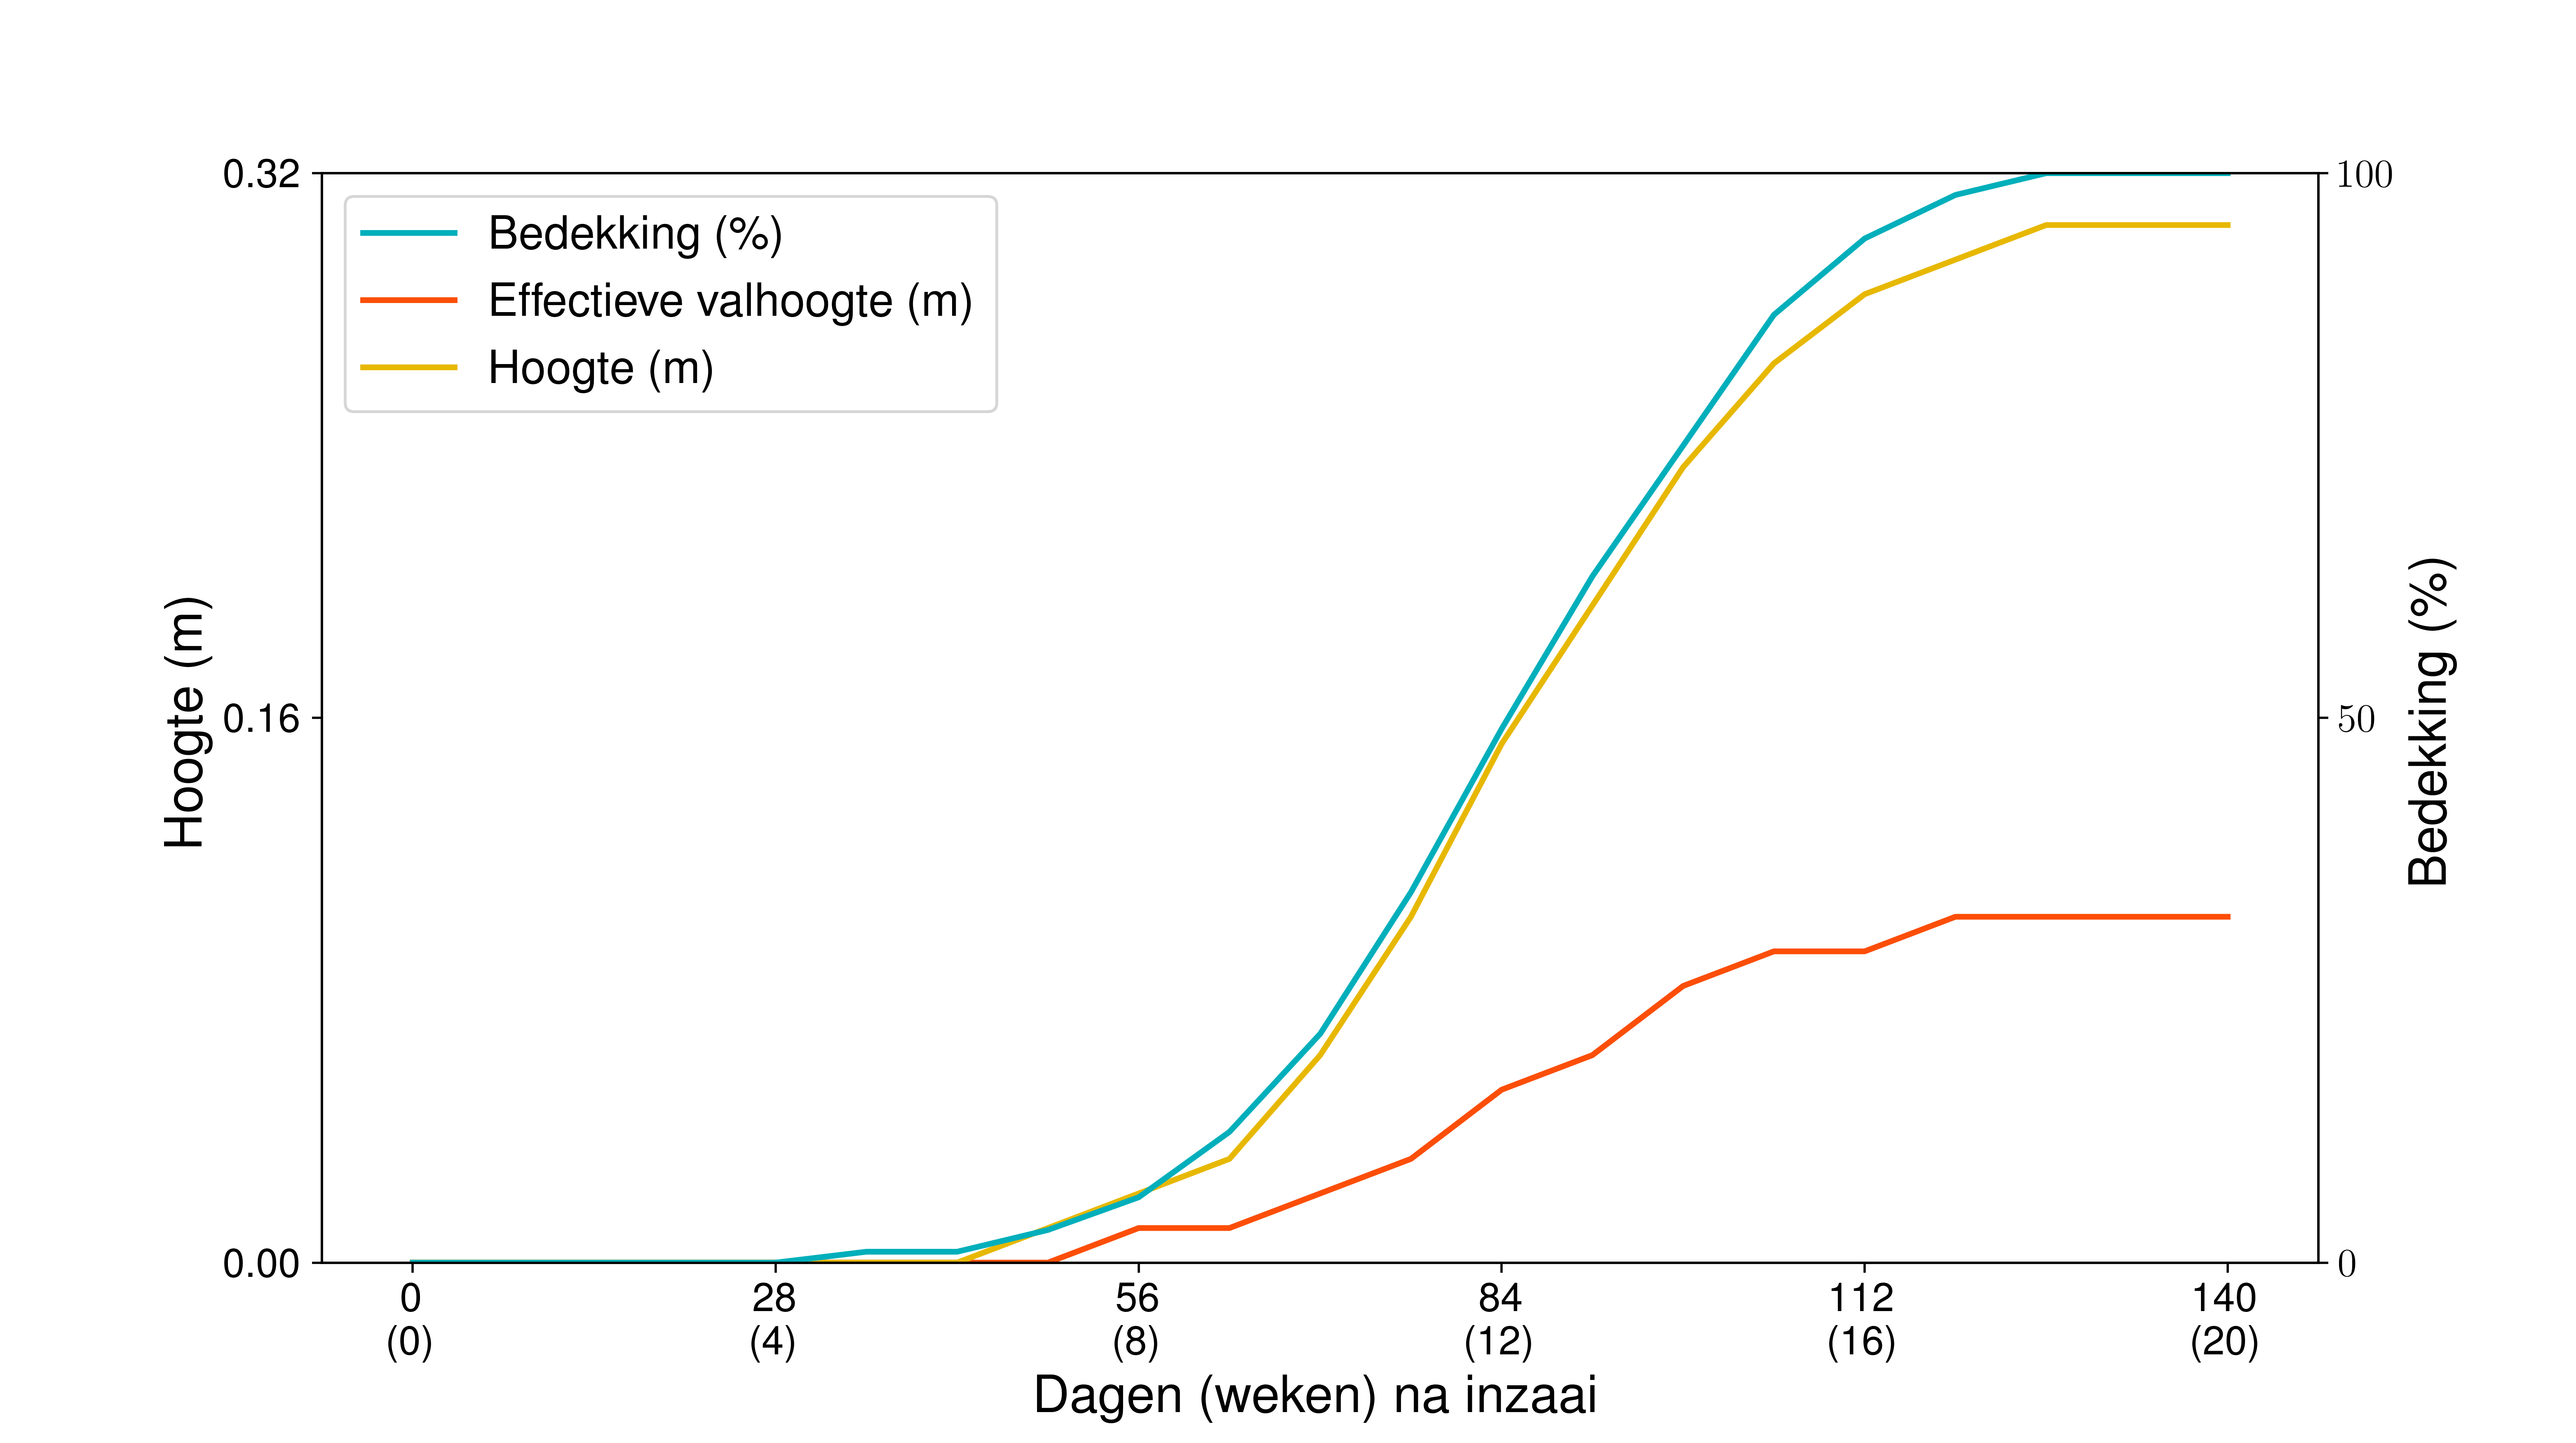
\includegraphics[width=12.5cm]{temp/1027.png} \end{figure} \end{center} 
  \textbf{Referenties:} ILVO2019;RUSLE \vspace{0.10cm} \\ 
  \textbf{Opmerkingen?} verloop gewasgroeicurves geinterpoleerd met cumulatieve stikstofopname curve geraporteerd in Coopman et al. (2013) \vspace{0.10cm} \\ 
 \newpage 
 \section{Wortel (vroege)  - vers (groep\_id 28)} 
 \textbf{Van toepassing op gewasnamen (en codes):} Wortel (vroege) (consumptie) - vers (9564) 
 \begin{multicols}{3} \begin{itemize} \item[$\square$] Meerjarig \item[$\square$] Groenbedekker \item[$\boxtimes$] Groente \end{itemize} \end{multicols} 
  \textbf{Zaaidatum (dd/mm)}: 25/02  \vspace{0.10cm} \\ 
  \textbf{Oogstdatum (dd/mm)}: 01/08  \vspace{0.10cm} \\ 
  \textbf{Oogstresten} \vspace{0.05cm} \\ 
  \tab Initi\"{e}le hoeveelheid (kg ha$^{-1}$): 2200.00 \vspace{0.05cm} \\ 
  \tab Afbraakcoefficient (-): 0.03 \vspace{0.05cm} \\ 
  \tab Bodembedekking (m$^2$ kg$^{-1}$): 4.18 \vspace{0.05cm} \\ 
  \tab Initieel percentage bedekking (\%): 60 \vspace{0.05cm} \\ 
  \tab Halfwaarde tijd (dagen): 10 \vspace{0.05cm} \\ 
  \textbf{Initi\"{e}le bodemruwheid (mm)}: 7.60 \vspace{0.05cm} \\ 
  \textbf{Gewasgroeicurve subgroep\_id 1027:} 
 \begin{center} \begin{figure}[H] 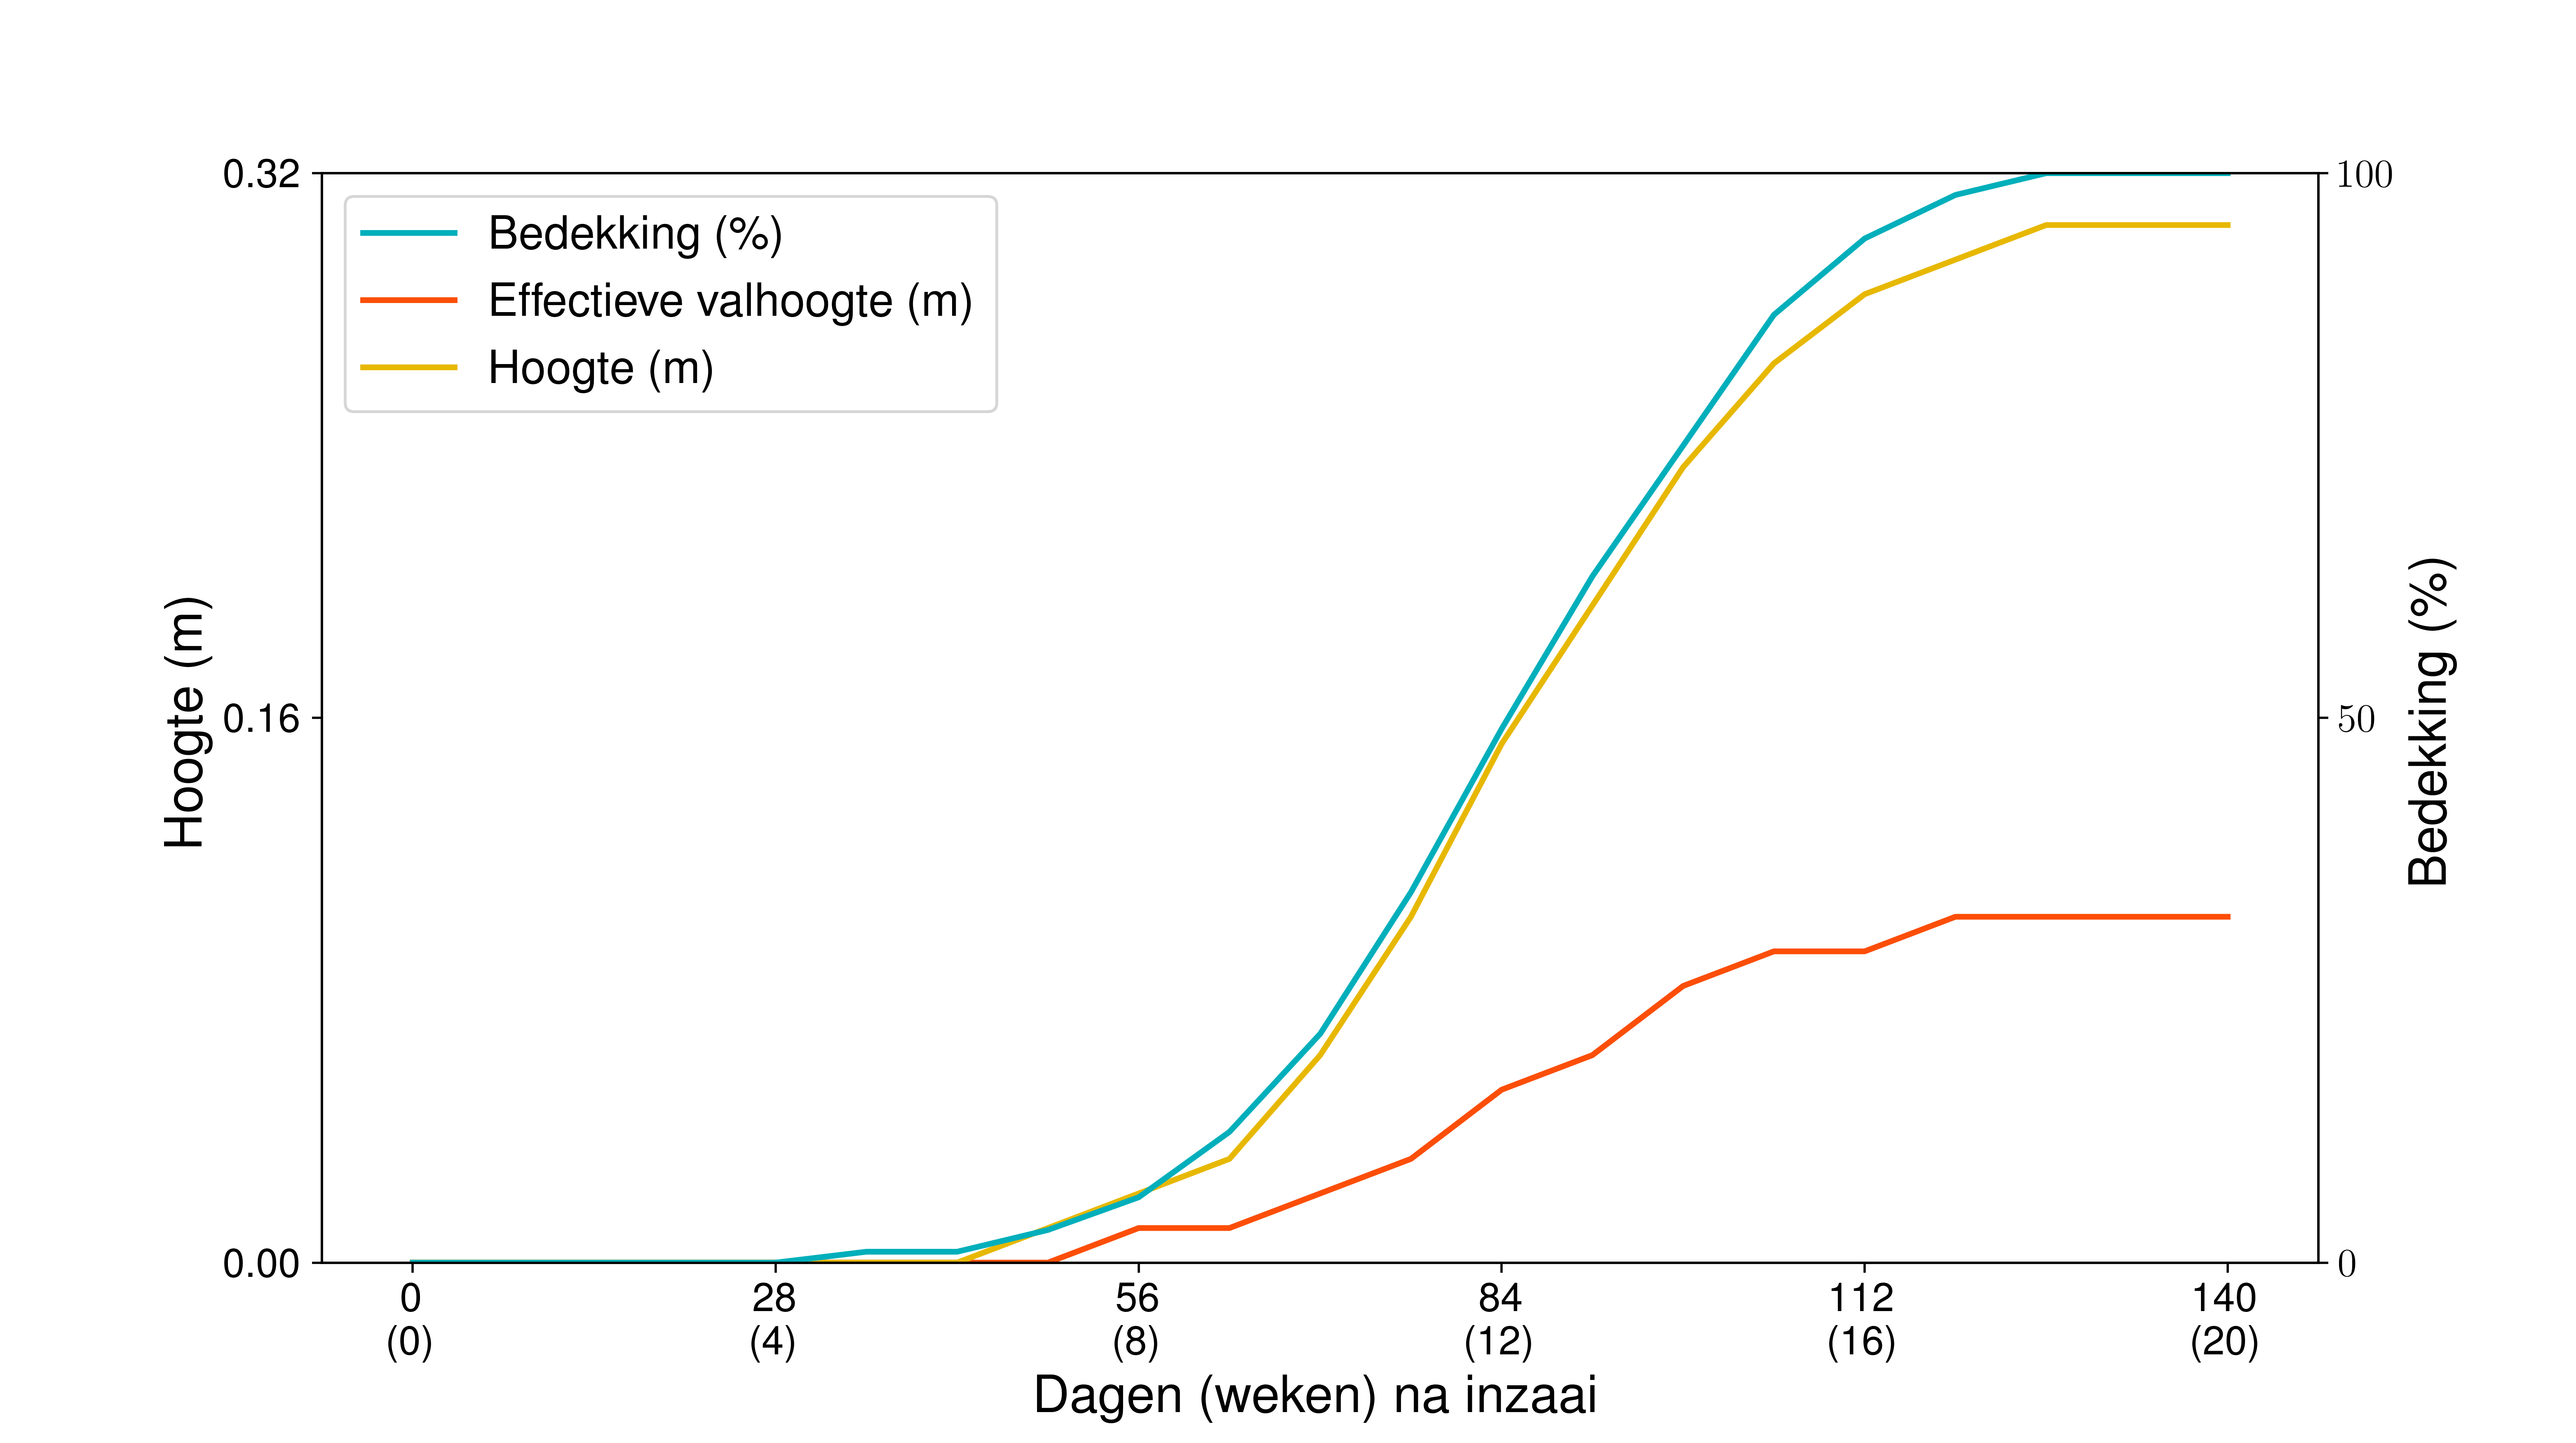
\includegraphics[width=12.5cm]{temp/1027.png} \end{figure} \end{center} 
  \textbf{Referenties:} ILVO2019;RUSLE \vspace{0.10cm} \\ 
  \textbf{Opmerkingen?} verloop gewasgroeicurves geinterpoleerd met cumulatieve stikstofopname curve geraporteerd in Coopman et al. (2013) \vspace{0.10cm} \\ 
 \newpage 
 \section{Wortel (niet-vroege) - industrie (groep\_id 29)} 
 \textbf{Van toepassing op gewasnamen (en codes):} Wortel (niet-vroege) (consumptie) - industrie (8535) 
 \begin{multicols}{3} \begin{itemize} \item[$\square$] Meerjarig \item[$\square$] Groenbedekker \item[$\boxtimes$] Groente \end{itemize} \end{multicols} 
  \textbf{Zaaidatum (dd/mm)}: 01/05  \vspace{0.10cm} \\ 
  \textbf{Oogstdatum (dd/mm)}: 15/11  \vspace{0.10cm} \\ 
  \textbf{Oogstresten} \vspace{0.05cm} \\ 
  \tab Initi\"{e}le hoeveelheid (kg ha$^{-1}$): 2200.00 \vspace{0.05cm} \\ 
  \tab Afbraakcoefficient (-): 0.03 \vspace{0.05cm} \\ 
  \tab Bodembedekking (m$^2$ kg$^{-1}$): 4.18 \vspace{0.05cm} \\ 
  \tab Initieel percentage bedekking (\%): 60 \vspace{0.05cm} \\ 
  \tab Halfwaarde tijd (dagen): 10 \vspace{0.05cm} \\ 
  \textbf{Initi\"{e}le bodemruwheid (mm)}: 7.60 \vspace{0.05cm} \\ 
  \textbf{Gewasgroeicurve subgroep\_id 1027:} 
 \begin{center} \begin{figure}[H] 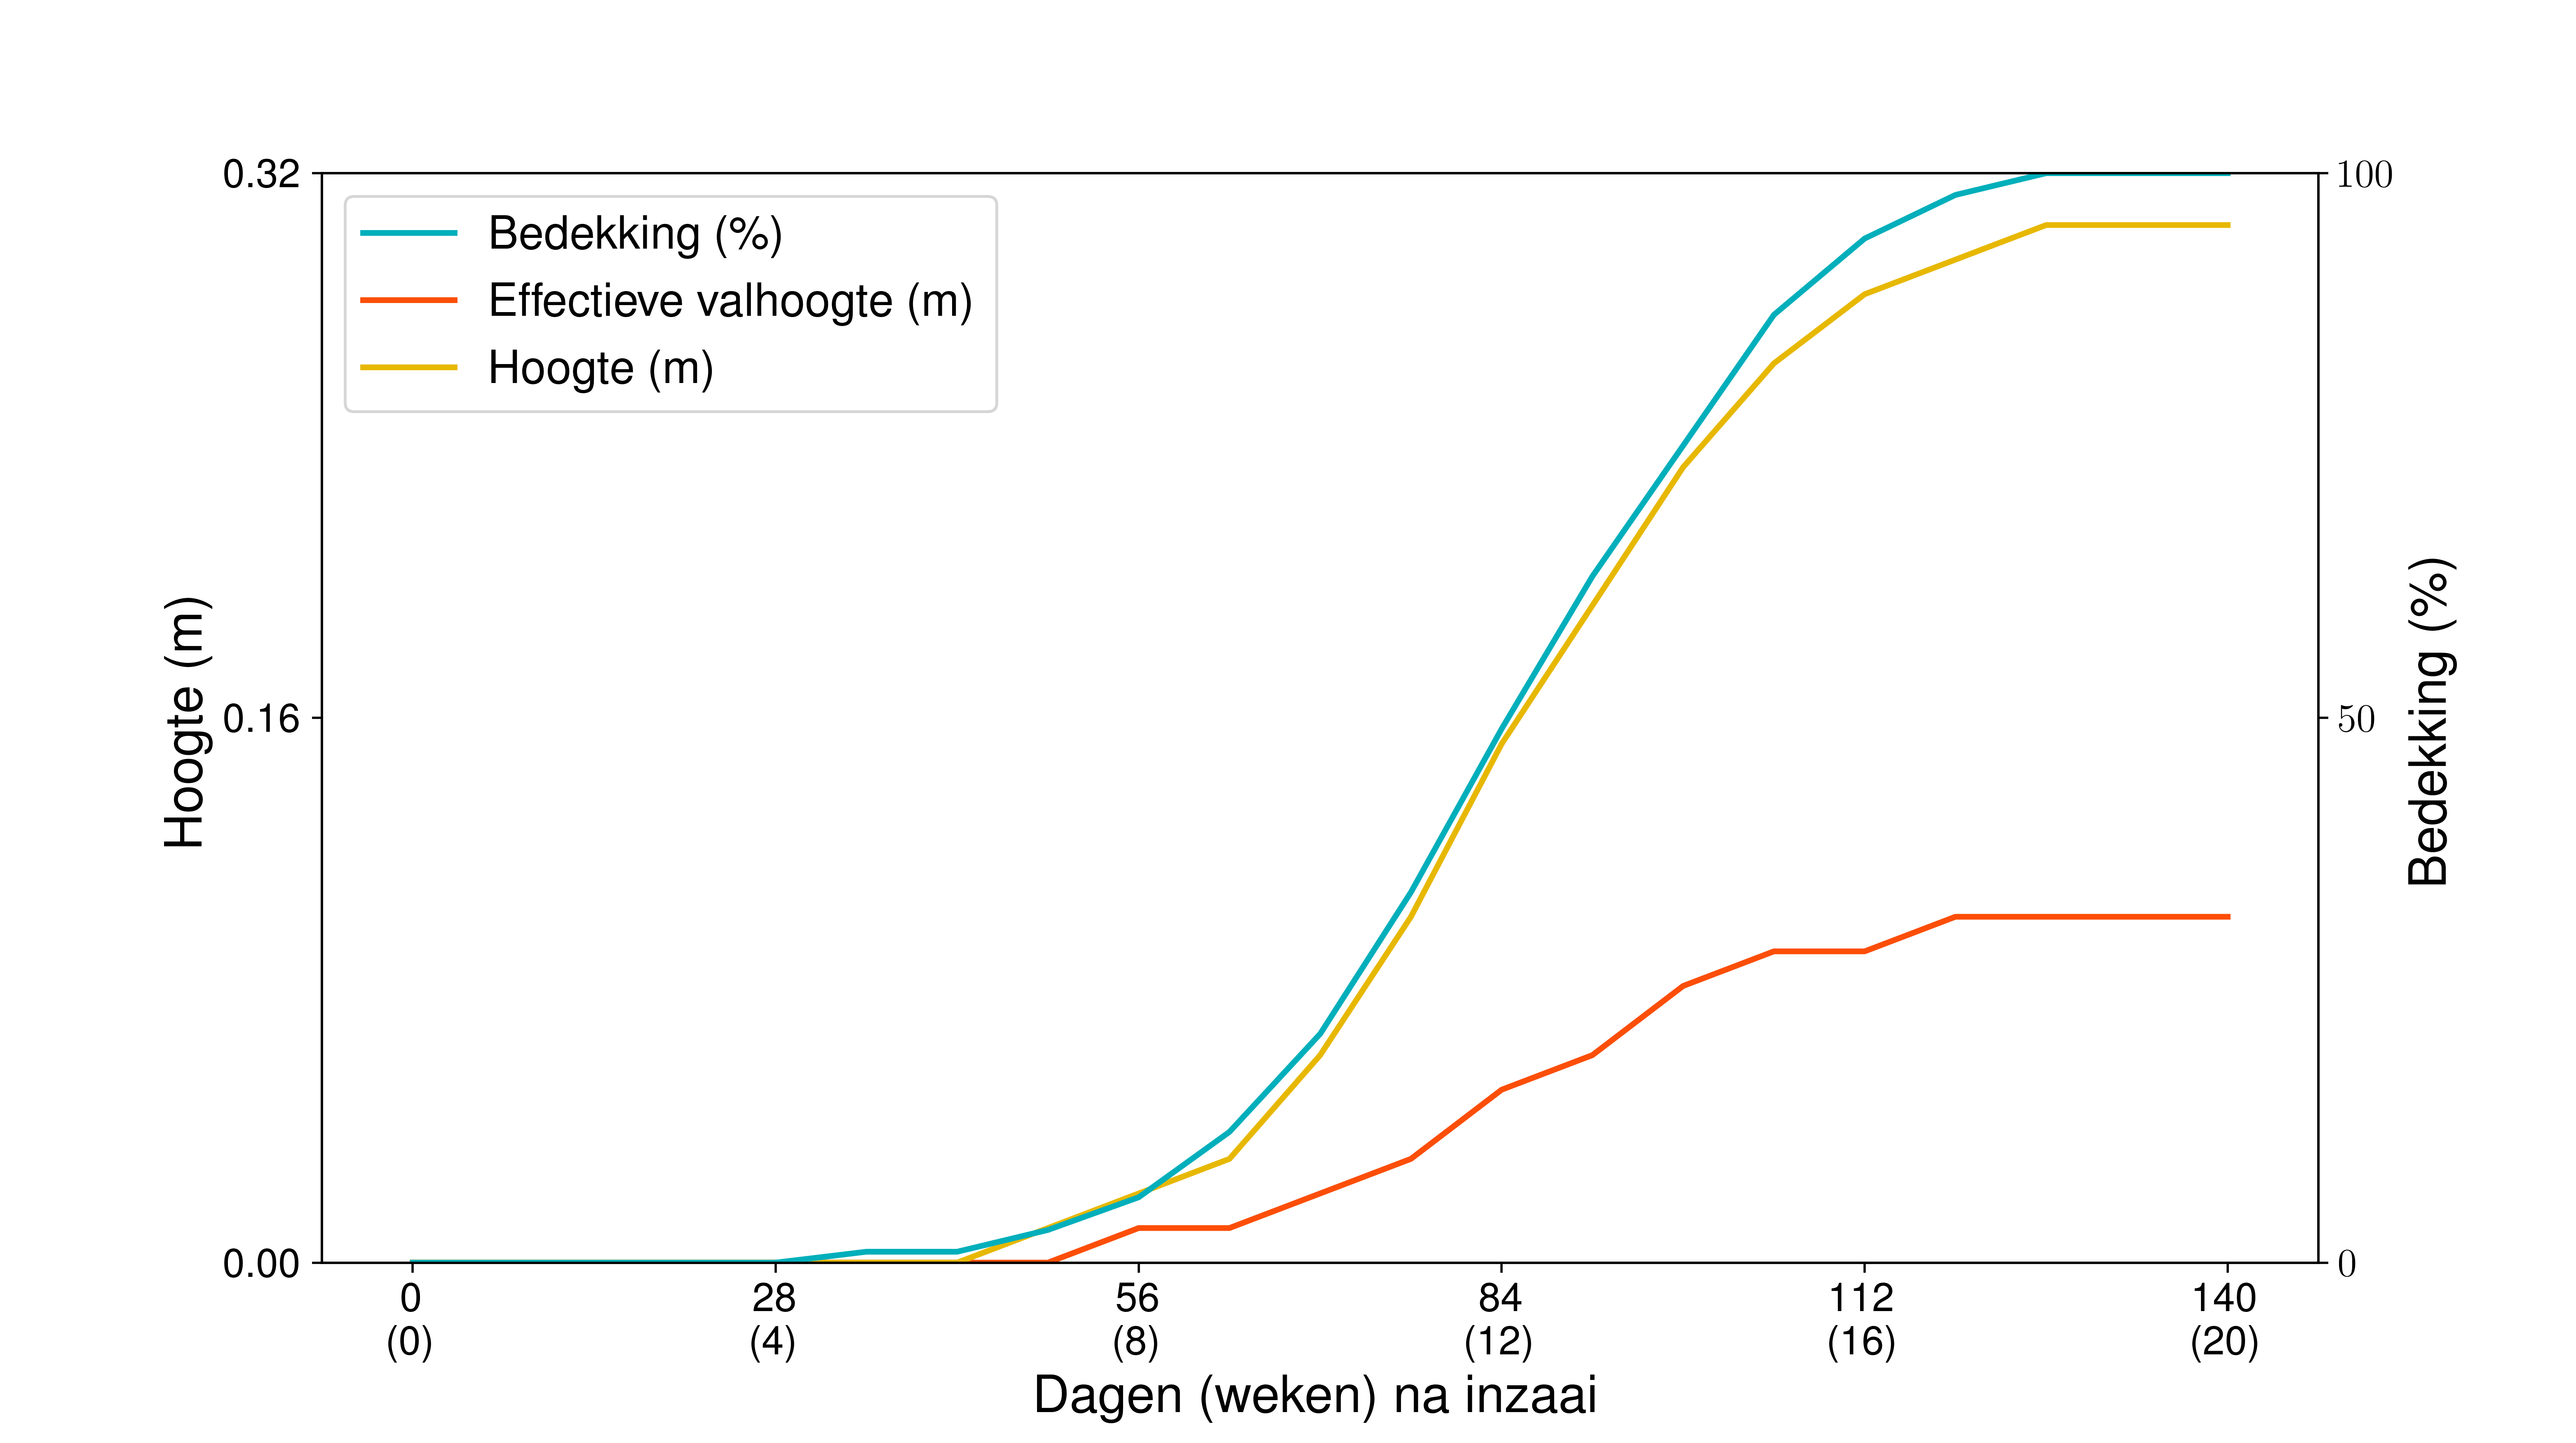
\includegraphics[width=12.5cm]{temp/1027.png} \end{figure} \end{center} 
  \textbf{Referenties:} ILVO2019;RUSLE \vspace{0.10cm} \\ 
  \textbf{Opmerkingen?} verloop gewasgroeicurves geinterpoleerd met cumulatieve stikstofopname curve geraporteerd in Coopman et al. (2013) \vspace{0.10cm} \\ 
 \newpage 
 \section{Wortel (niet-vroege) - vers (groep\_id 30)} 
 \textbf{Van toepassing op gewasnamen (en codes):} Wortel (niet-vroege) (consumptie) - vers (9535) 
 \begin{multicols}{3} \begin{itemize} \item[$\square$] Meerjarig \item[$\square$] Groenbedekker \item[$\boxtimes$] Groente \end{itemize} \end{multicols} 
  \textbf{Zaaidatum (dd/mm)}: 01/05  \vspace{0.10cm} \\ 
  \textbf{Oogstdatum (dd/mm)}: 25/10  \vspace{0.10cm} \\ 
  \textbf{Oogstresten} \vspace{0.05cm} \\ 
  \tab Initi\"{e}le hoeveelheid (kg ha$^{-1}$): 2200.00 \vspace{0.05cm} \\ 
  \tab Afbraakcoefficient (-): 0.03 \vspace{0.05cm} \\ 
  \tab Bodembedekking (m$^2$ kg$^{-1}$): 4.18 \vspace{0.05cm} \\ 
  \tab Initieel percentage bedekking (\%): 60 \vspace{0.05cm} \\ 
  \tab Halfwaarde tijd (dagen): 10 \vspace{0.05cm} \\ 
  \textbf{Initi\"{e}le bodemruwheid (mm)}: 7.60 \vspace{0.05cm} \\ 
  \textbf{Gewasgroeicurve subgroep\_id 1027:} 
 \begin{center} \begin{figure}[H] 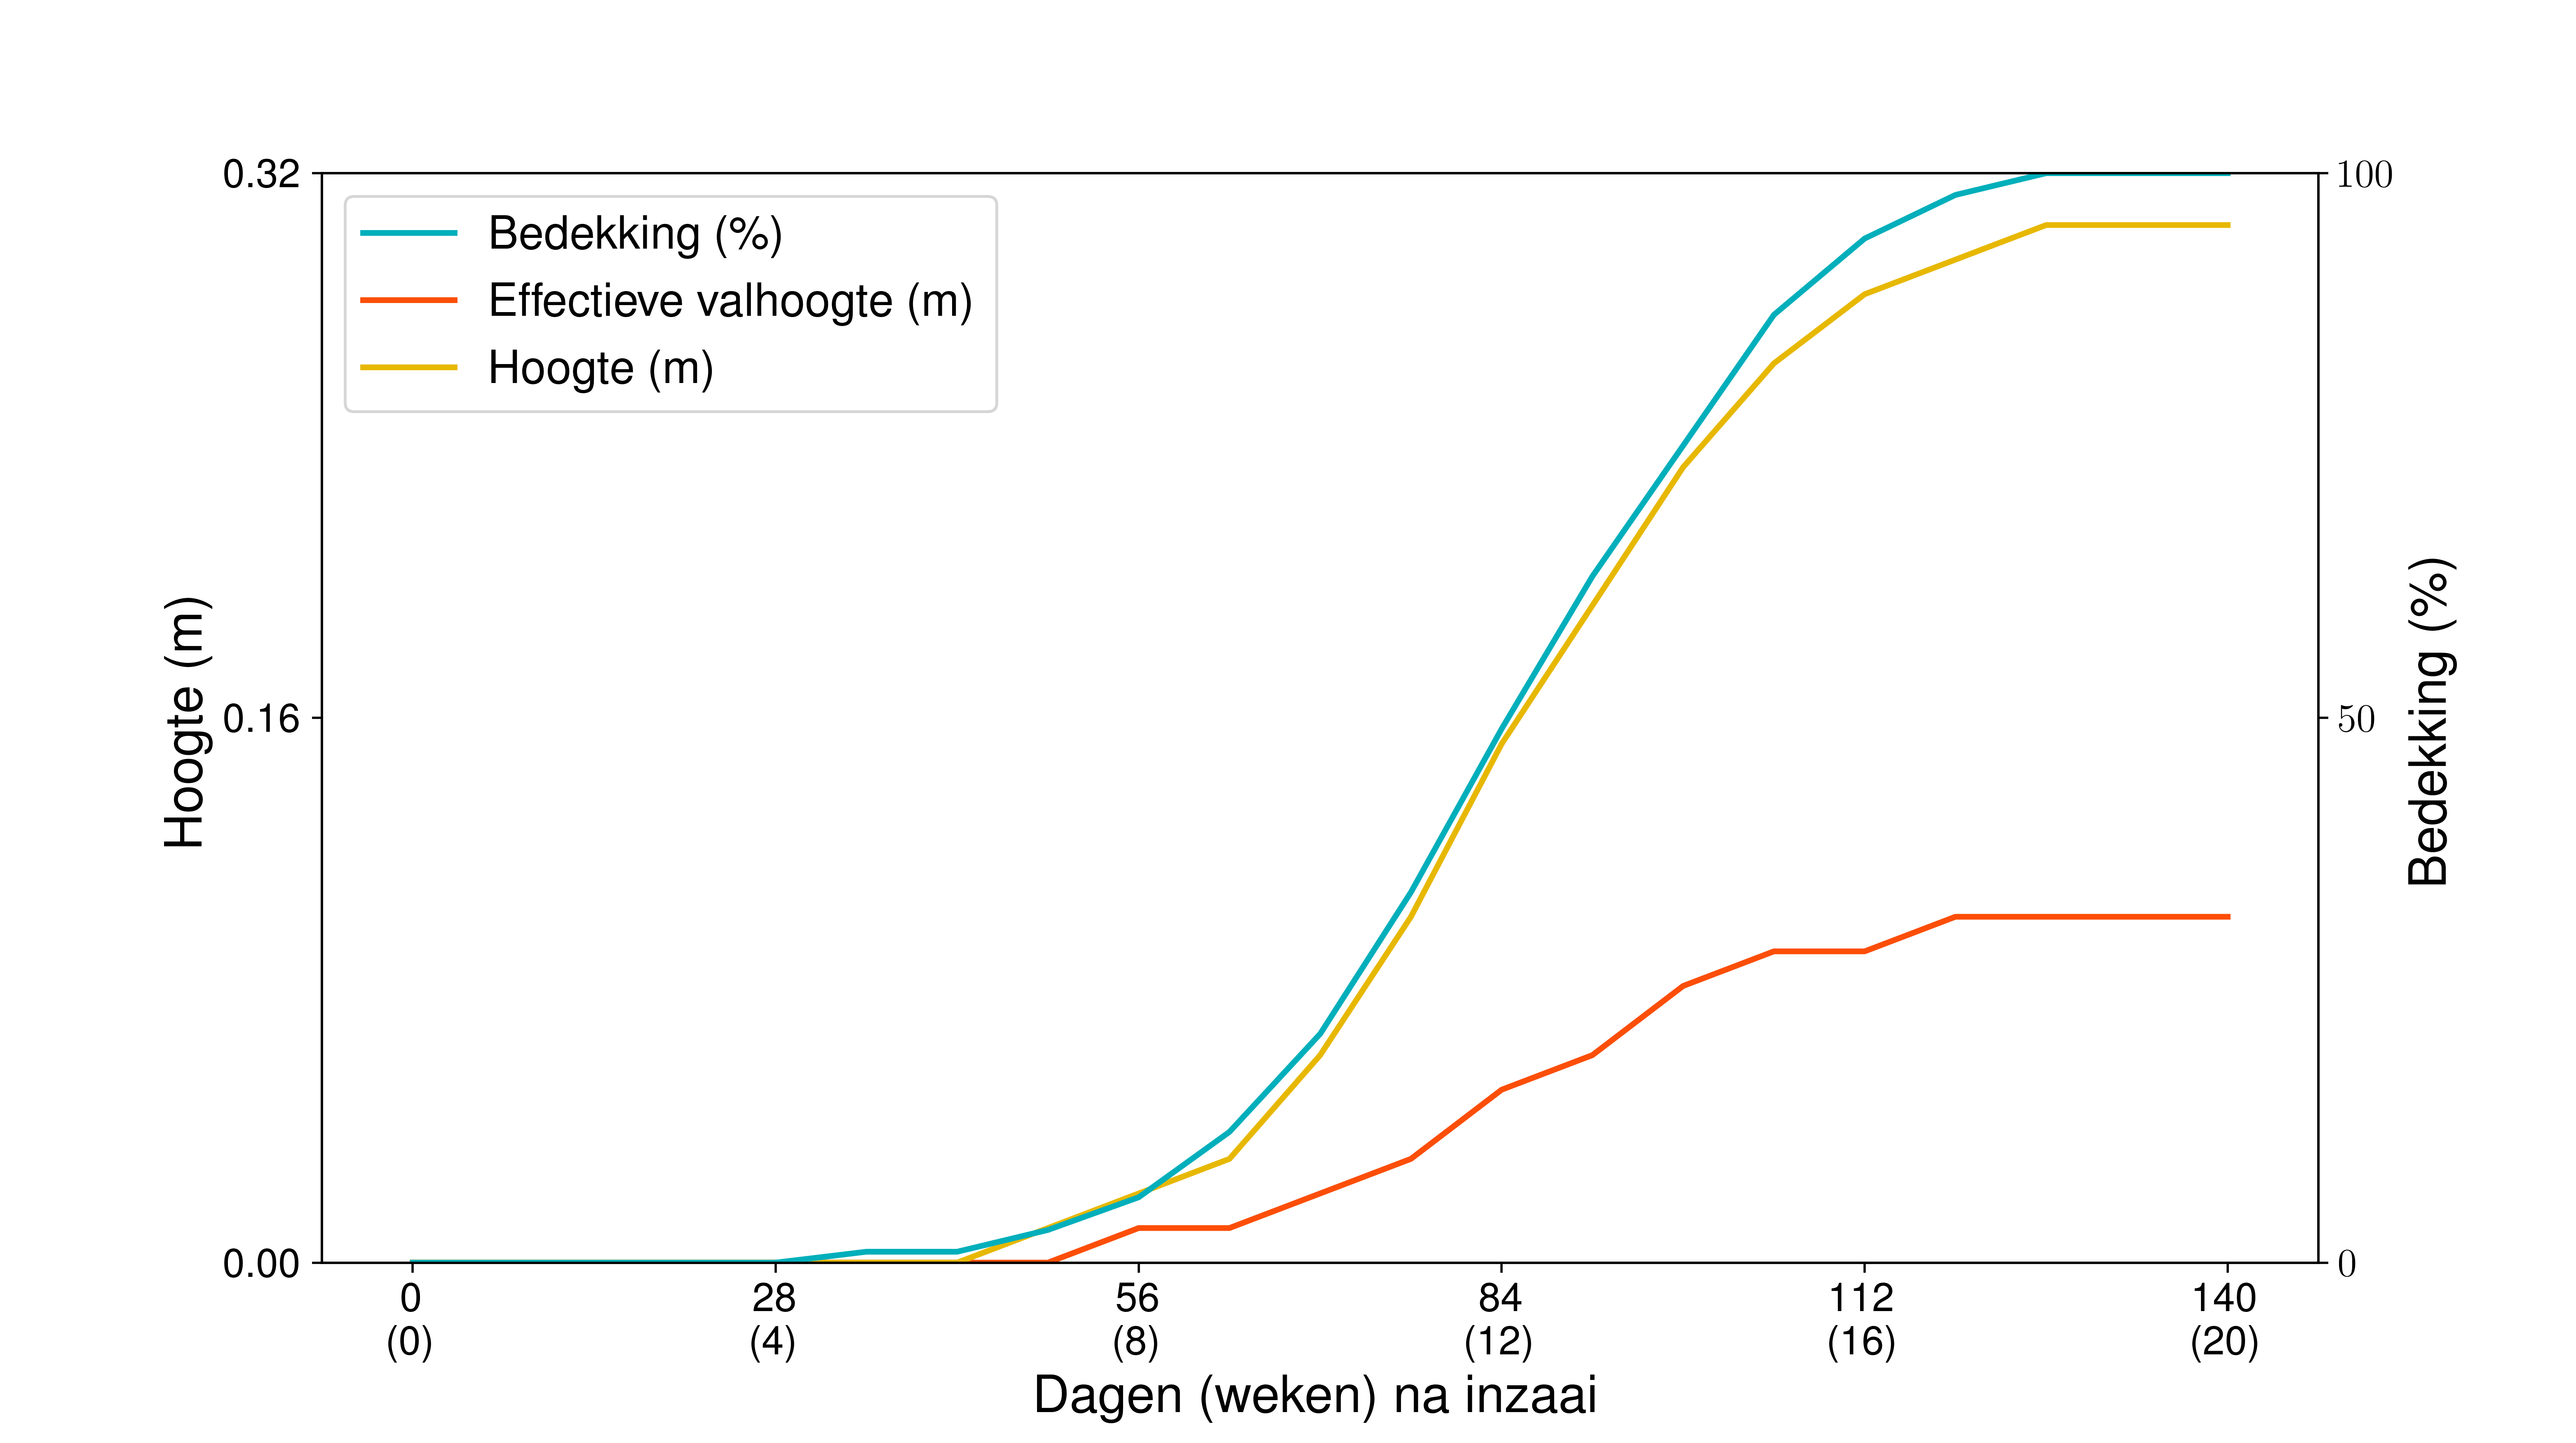
\includegraphics[width=12.5cm]{temp/1027.png} \end{figure} \end{center} 
  \textbf{Referenties:} ILVO2019;RUSLE \vspace{0.10cm} \\ 
  \textbf{Opmerkingen?} verloop gewasgroeicurves geinterpoleerd met cumulatieve stikstofopname curve geraporteerd in Coopman et al. (2013) \vspace{0.10cm} \\ 
 \newpage 
 \section{Cichorei (inuline) (groep\_id 31)} 
 \textbf{Van toepassing op gewasnamen (en codes):} Cichorei (inuline) (9811) 
 \begin{multicols}{3} \begin{itemize} \item[$\square$] Meerjarig \item[$\square$] Groenbedekker \item[$\boxtimes$] Groente \end{itemize} \end{multicols} 
  \textbf{Zaaidatum (dd/mm)}: 15/04  \vspace{0.10cm} \\ 
  \textbf{Oogstdatum (dd/mm)}: 15/10  \vspace{0.10cm} \\ 
  \textbf{Oogstresten} \vspace{0.05cm} \\ 
  \tab Initi\"{e}le hoeveelheid (kg ha$^{-1}$): 1000.00 \vspace{0.05cm} \\ 
  \tab Afbraakcoefficient (-): 0.03 \vspace{0.05cm} \\ 
  \tab Bodembedekking (m$^2$ kg$^{-1}$): 2.23 \vspace{0.05cm} \\ 
  \tab Initieel percentage bedekking (\%): 20 \vspace{0.05cm} \\ 
  \tab Halfwaarde tijd (dagen): 10 \vspace{0.05cm} \\ 
  \textbf{Initi\"{e}le bodemruwheid (mm)}: 6.10 \vspace{0.05cm} \\ 
  \textbf{Gewasgroeicurve subgroep\_id 1031:} 
 \begin{center} \begin{figure}[H] 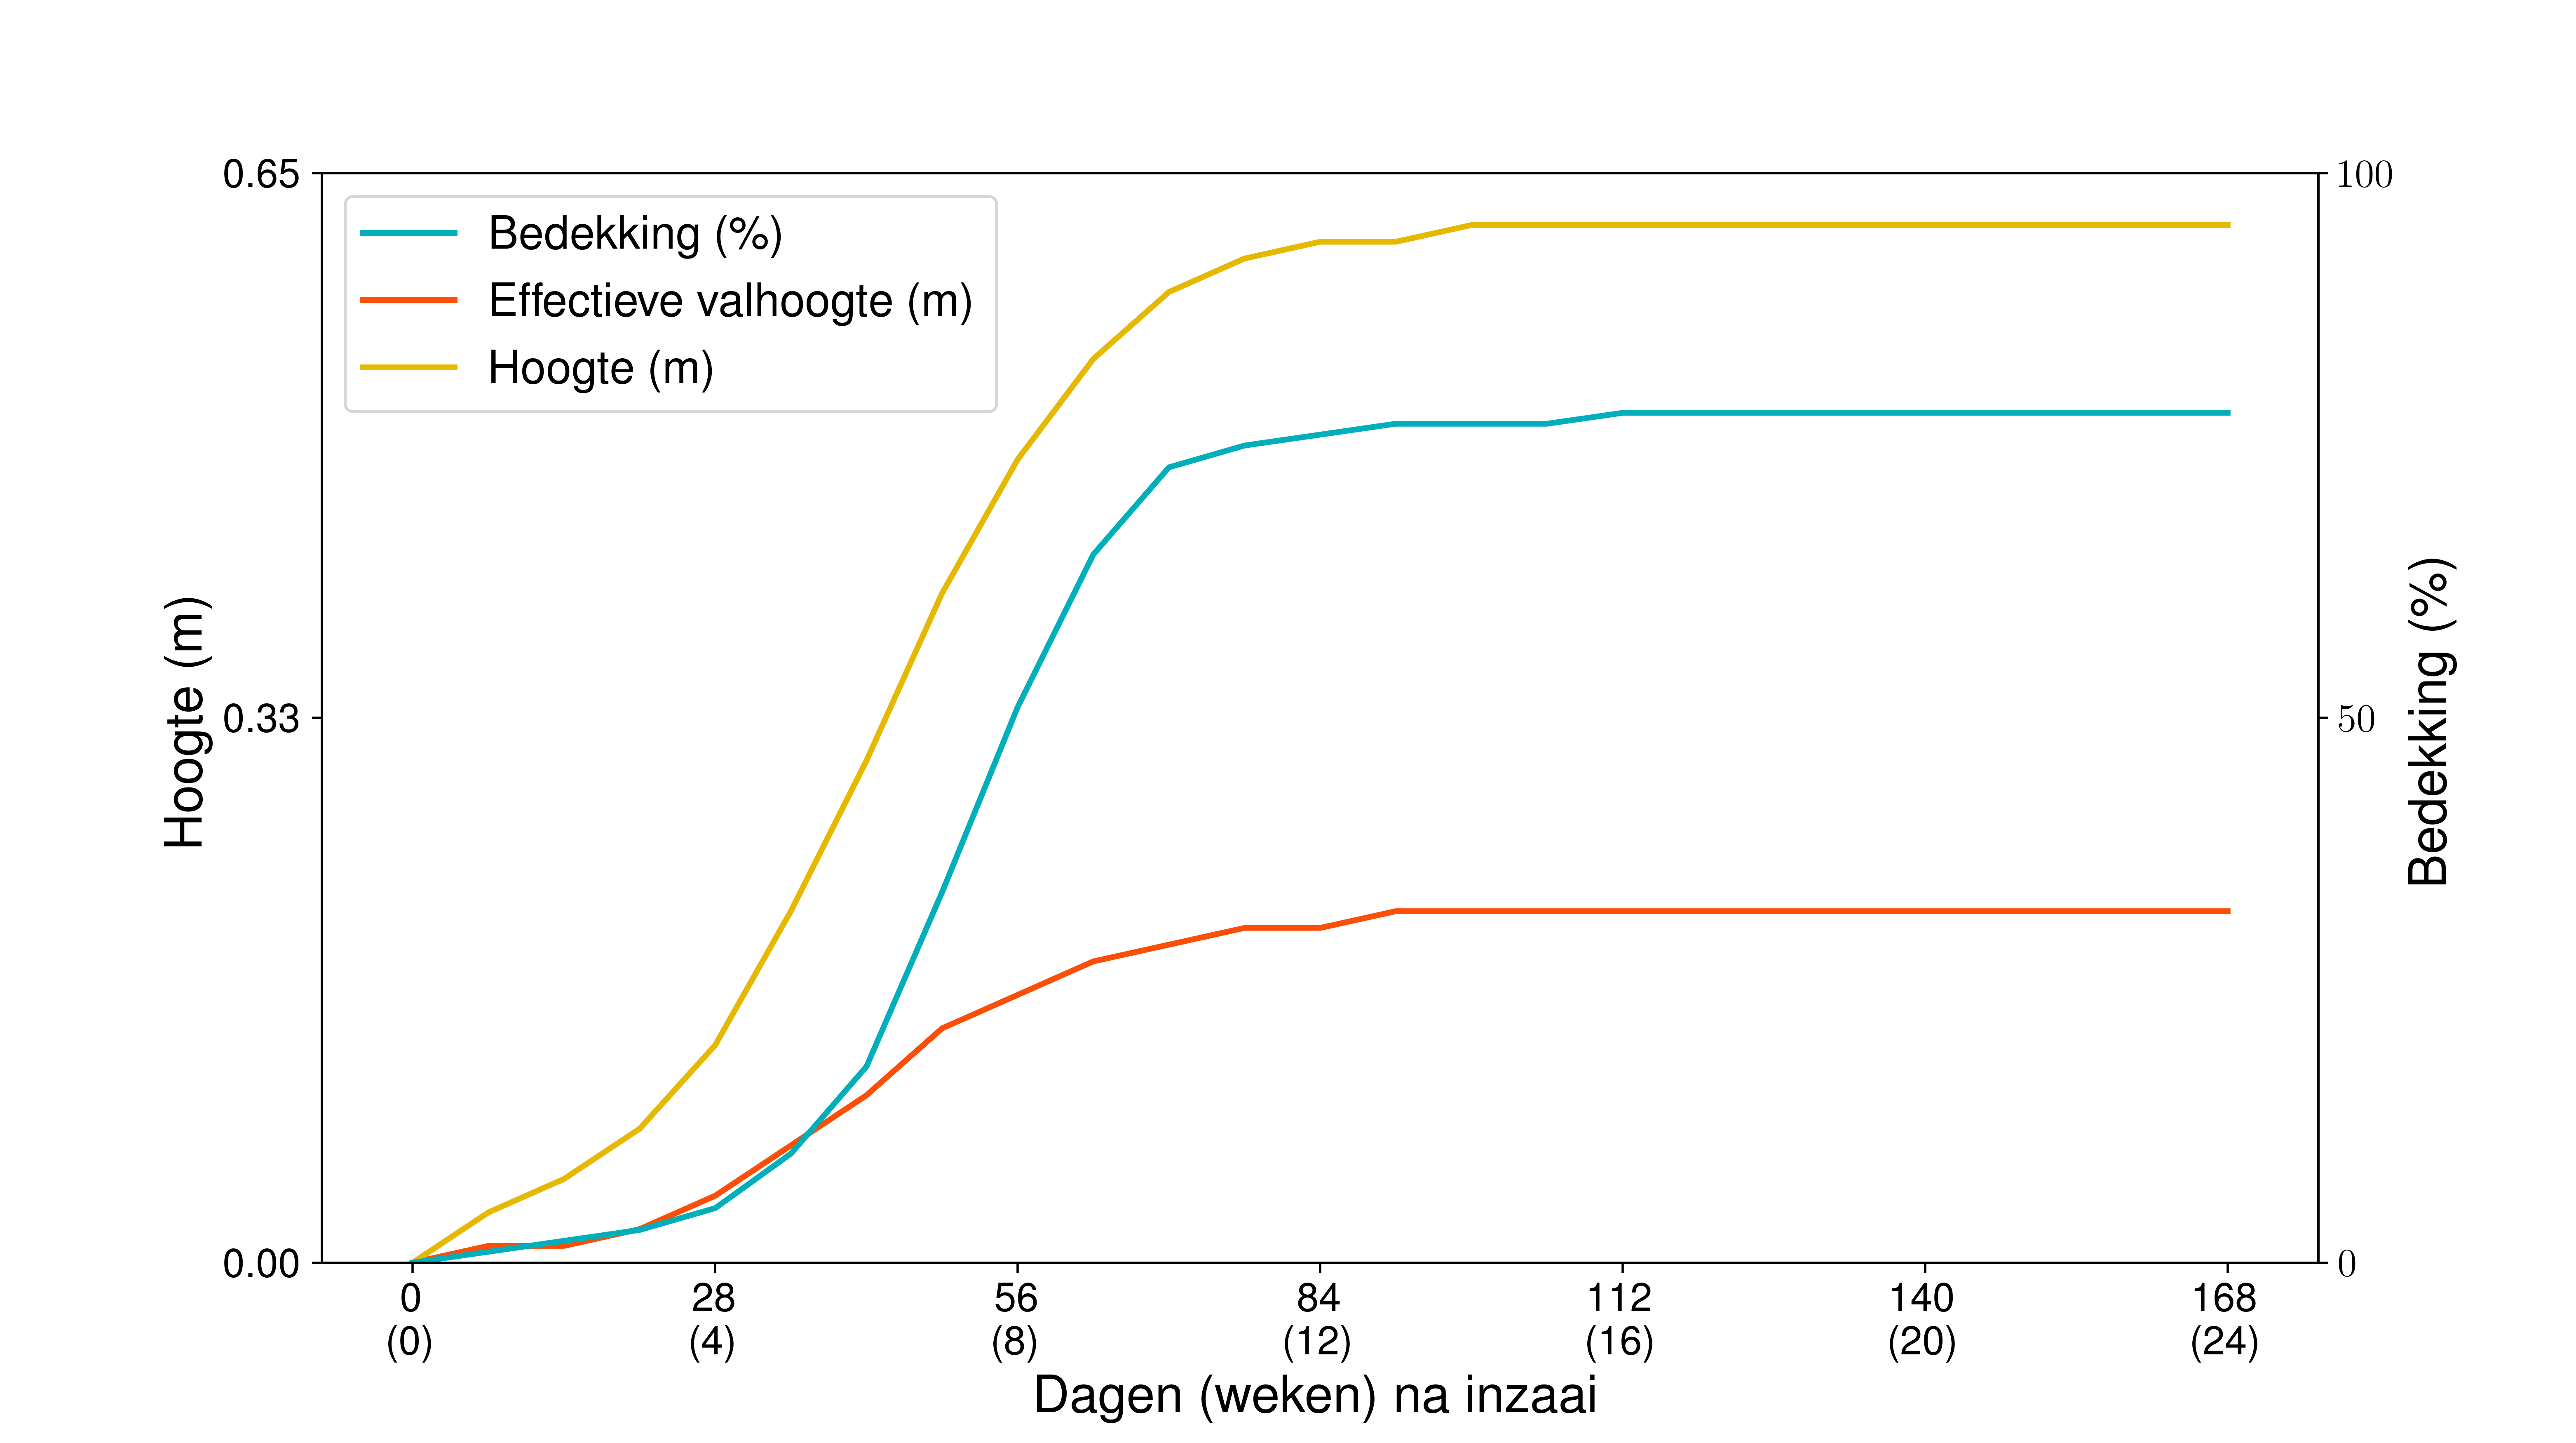
\includegraphics[width=12.5cm]{temp/1031.png} \end{figure} \end{center} 
  \textbf{Referenties:} ILVO2019 \vspace{0.10cm} \\ 
  \textbf{Opmerkingen?} geen \vspace{0.10cm} \\ 
 \newpage 
 \section{Witloofwortel (groep\_id 32)} 
 \textbf{Van toepassing op gewasnamen (en codes):} Witloofwortel (9561) 
 \begin{multicols}{3} \begin{itemize} \item[$\square$] Meerjarig \item[$\square$] Groenbedekker \item[$\boxtimes$] Groente \end{itemize} \end{multicols} 
  \textbf{Zaaidatum (dd/mm)}: 15/05  \vspace{0.10cm} \\ 
  \textbf{Oogstdatum (dd/mm)}: 25/10  \vspace{0.10cm} \\ 
  \textbf{Oogstresten} \vspace{0.05cm} \\ 
  \tab Initi\"{e}le hoeveelheid (kg ha$^{-1}$): 2019.00 \vspace{0.05cm} \\ 
  \tab Afbraakcoefficient (-): 0.01 \vspace{0.05cm} \\ 
  \tab Bodembedekking (m$^2$ kg$^{-1}$): 4.46 \vspace{0.05cm} \\ 
  \tab Initieel percentage bedekking (\%): 59 \vspace{0.05cm} \\ 
  \tab Halfwaarde tijd (dagen): 30 \vspace{0.05cm} \\ 
  \textbf{Initi\"{e}le bodemruwheid (mm)}: 7.60 \vspace{0.05cm} \\ 
  \textbf{Gewasgroeicurve subgroep\_id 1032:} 
 \begin{center} \begin{figure}[H] 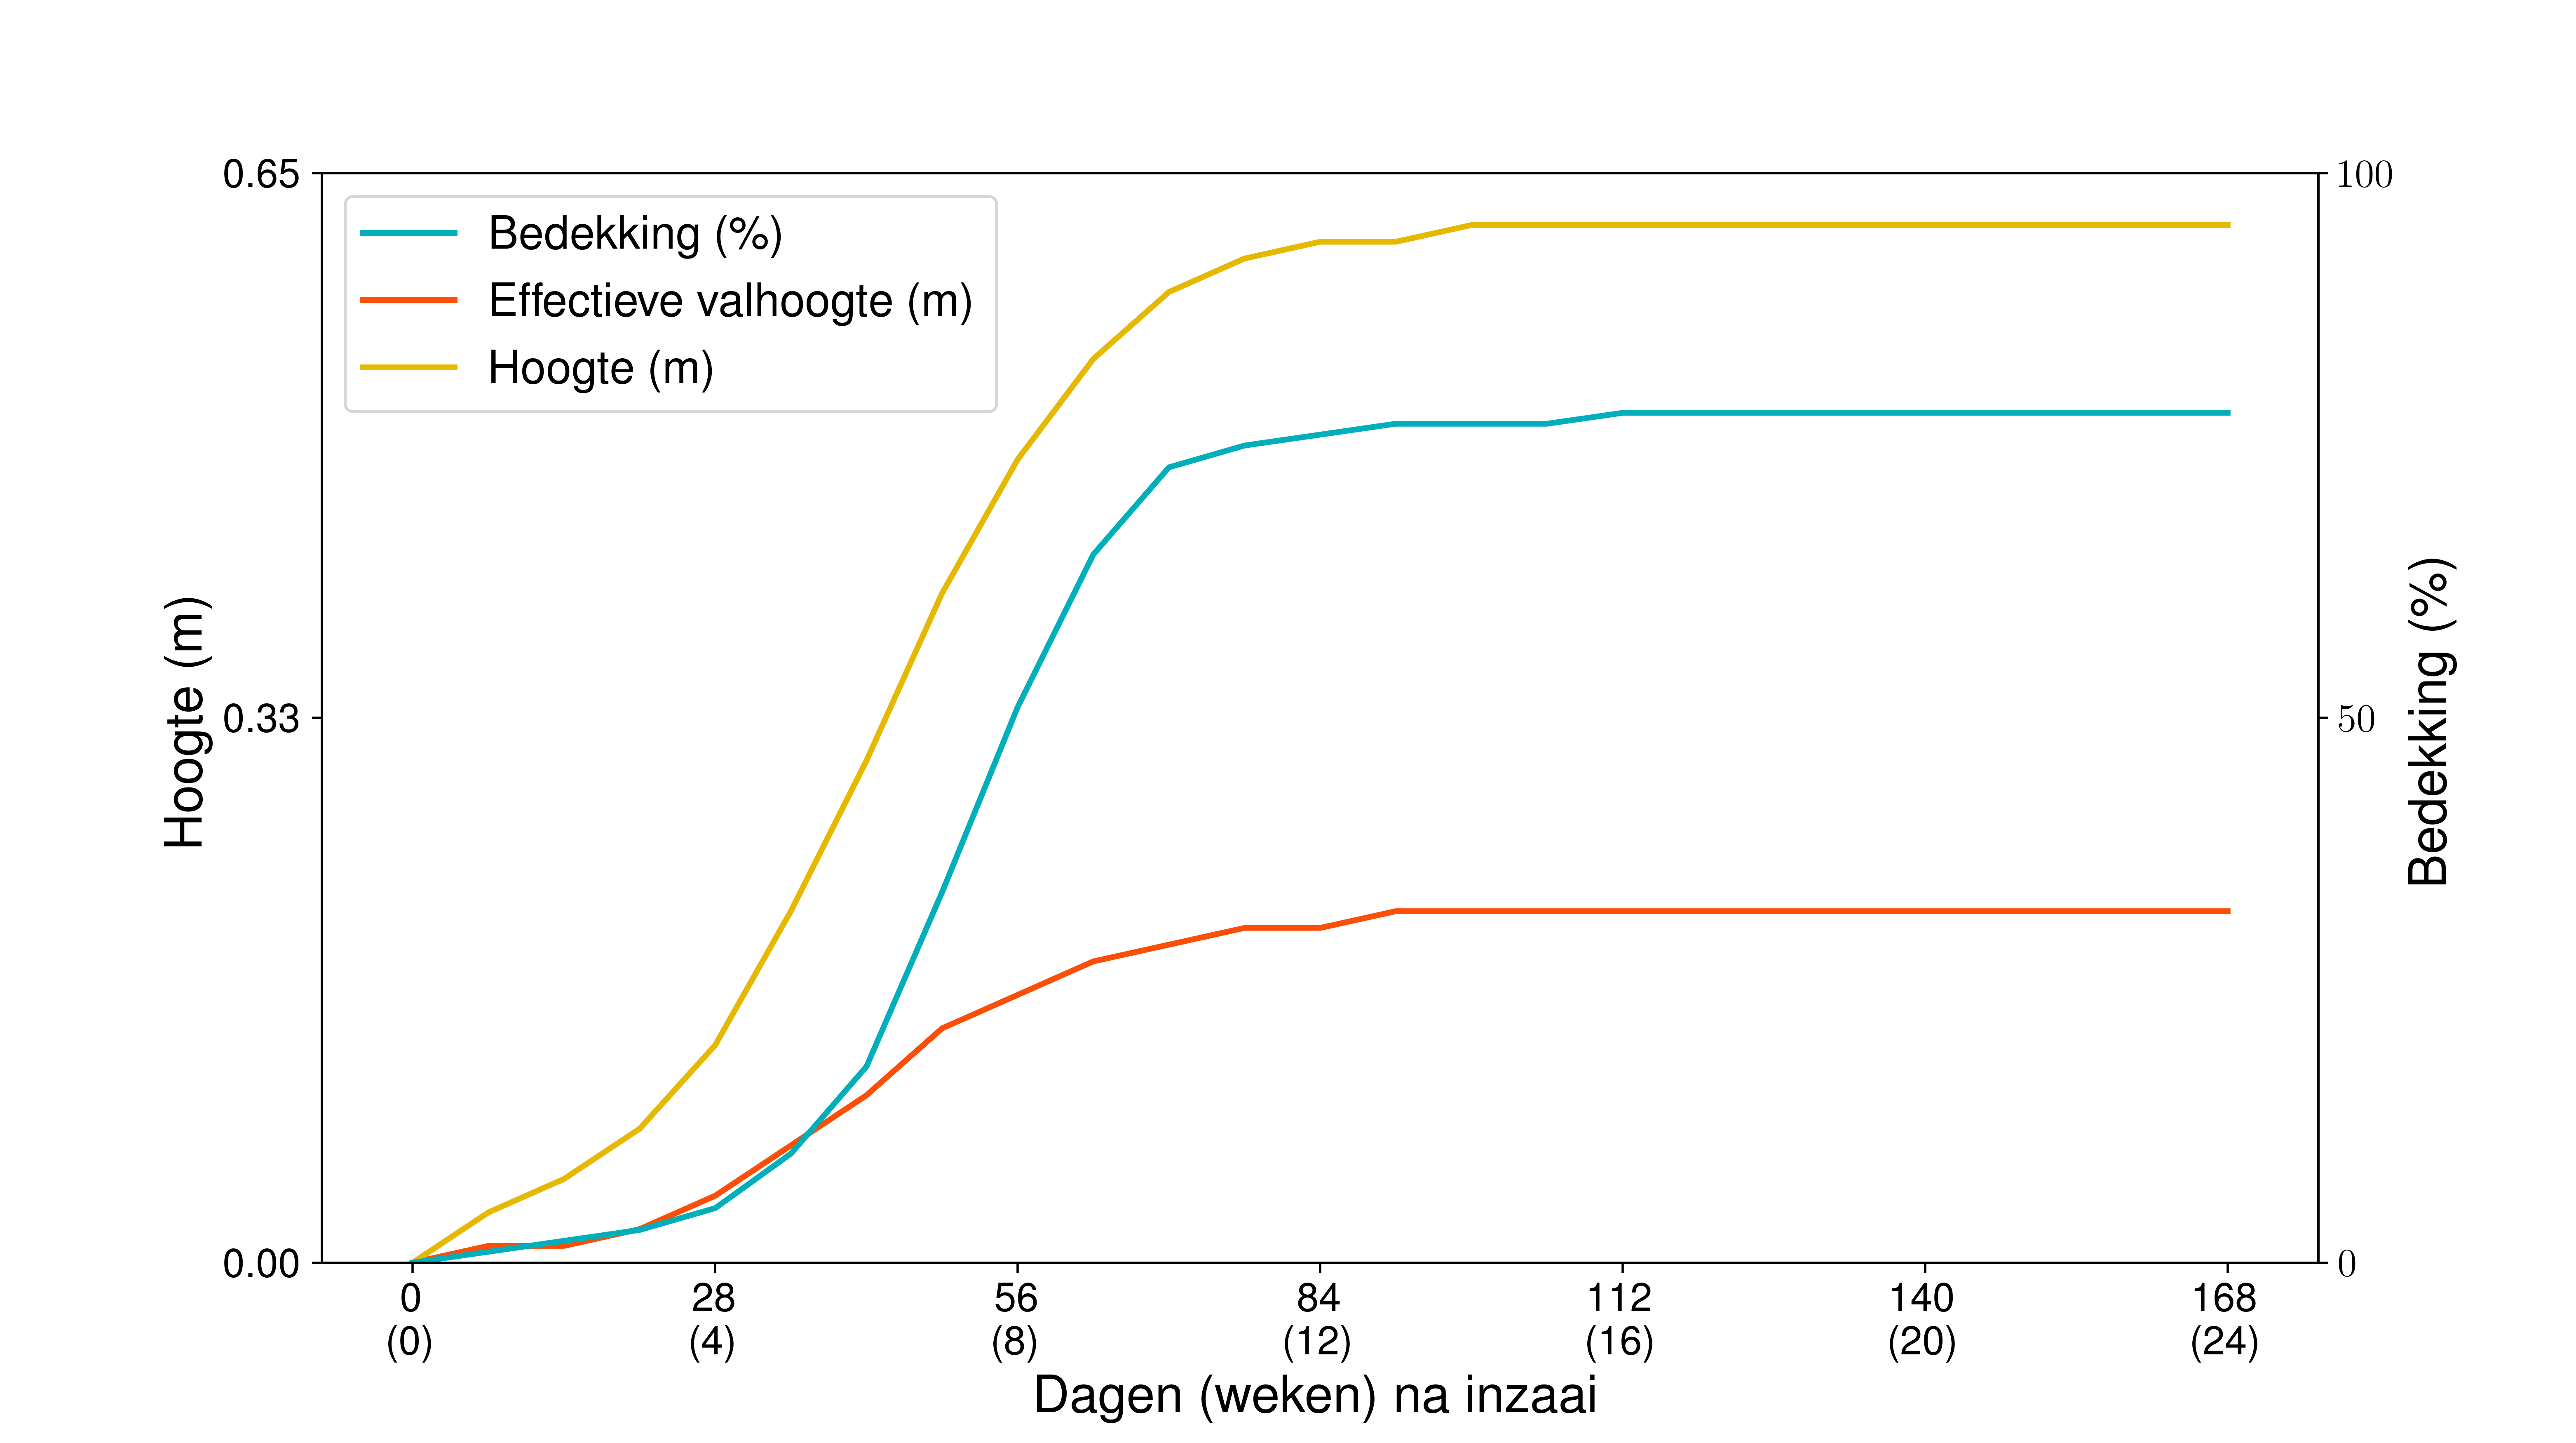
\includegraphics[width=12.5cm]{temp/1032.png} \end{figure} \end{center} 
  \textbf{Referenties:} Gabriels2003;ILVO2019 \vspace{0.10cm} \\ 
  \textbf{Opmerkingen?} geen \vspace{0.10cm} \\ 
 \newpage 
 \section{Prei (groep\_id 33)} 
 \textbf{Van toepassing op gewasnamen (en codes):} Prei - industrie (8538) , Prei - vers (9538) 
 \begin{multicols}{3} \begin{itemize} \item[$\square$] Meerjarig \item[$\square$] Groenbedekker \item[$\boxtimes$] Groente \end{itemize} \end{multicols} 
 \subsection{Voorteelt (subgroep\_id 1033)} 
  \textbf{Zaaidatum (dd/mm)}: 15/03  \vspace{0.10cm} \\ 
  \textbf{Oogstdatum (dd/mm)}: 15/07  \vspace{0.10cm} \\ 
  \textbf{Oogstresten} \vspace{0.05cm} \\ 
  \tab Initi\"{e}le hoeveelheid (kg ha$^{-1}$): 3500.00 \vspace{0.05cm} \\ 
  \tab Afbraakcoefficient (-): 0.03 \vspace{0.05cm} \\ 
  \tab Bodembedekking (m$^2$ kg$^{-1}$): 1.07 \vspace{0.05cm} \\ 
  \tab Initieel percentage bedekking (\%): 28 \vspace{0.05cm} \\ 
  \tab Halfwaarde tijd (dagen): 10 \vspace{0.05cm} \\ 
  \textbf{Initi\"{e}le bodemruwheid (mm)}: 6.10 \vspace{0.05cm} \\ 
  \textbf{Gewasgroeicurve subgroep\_id 1033:} 
 \begin{center} \begin{figure}[H] 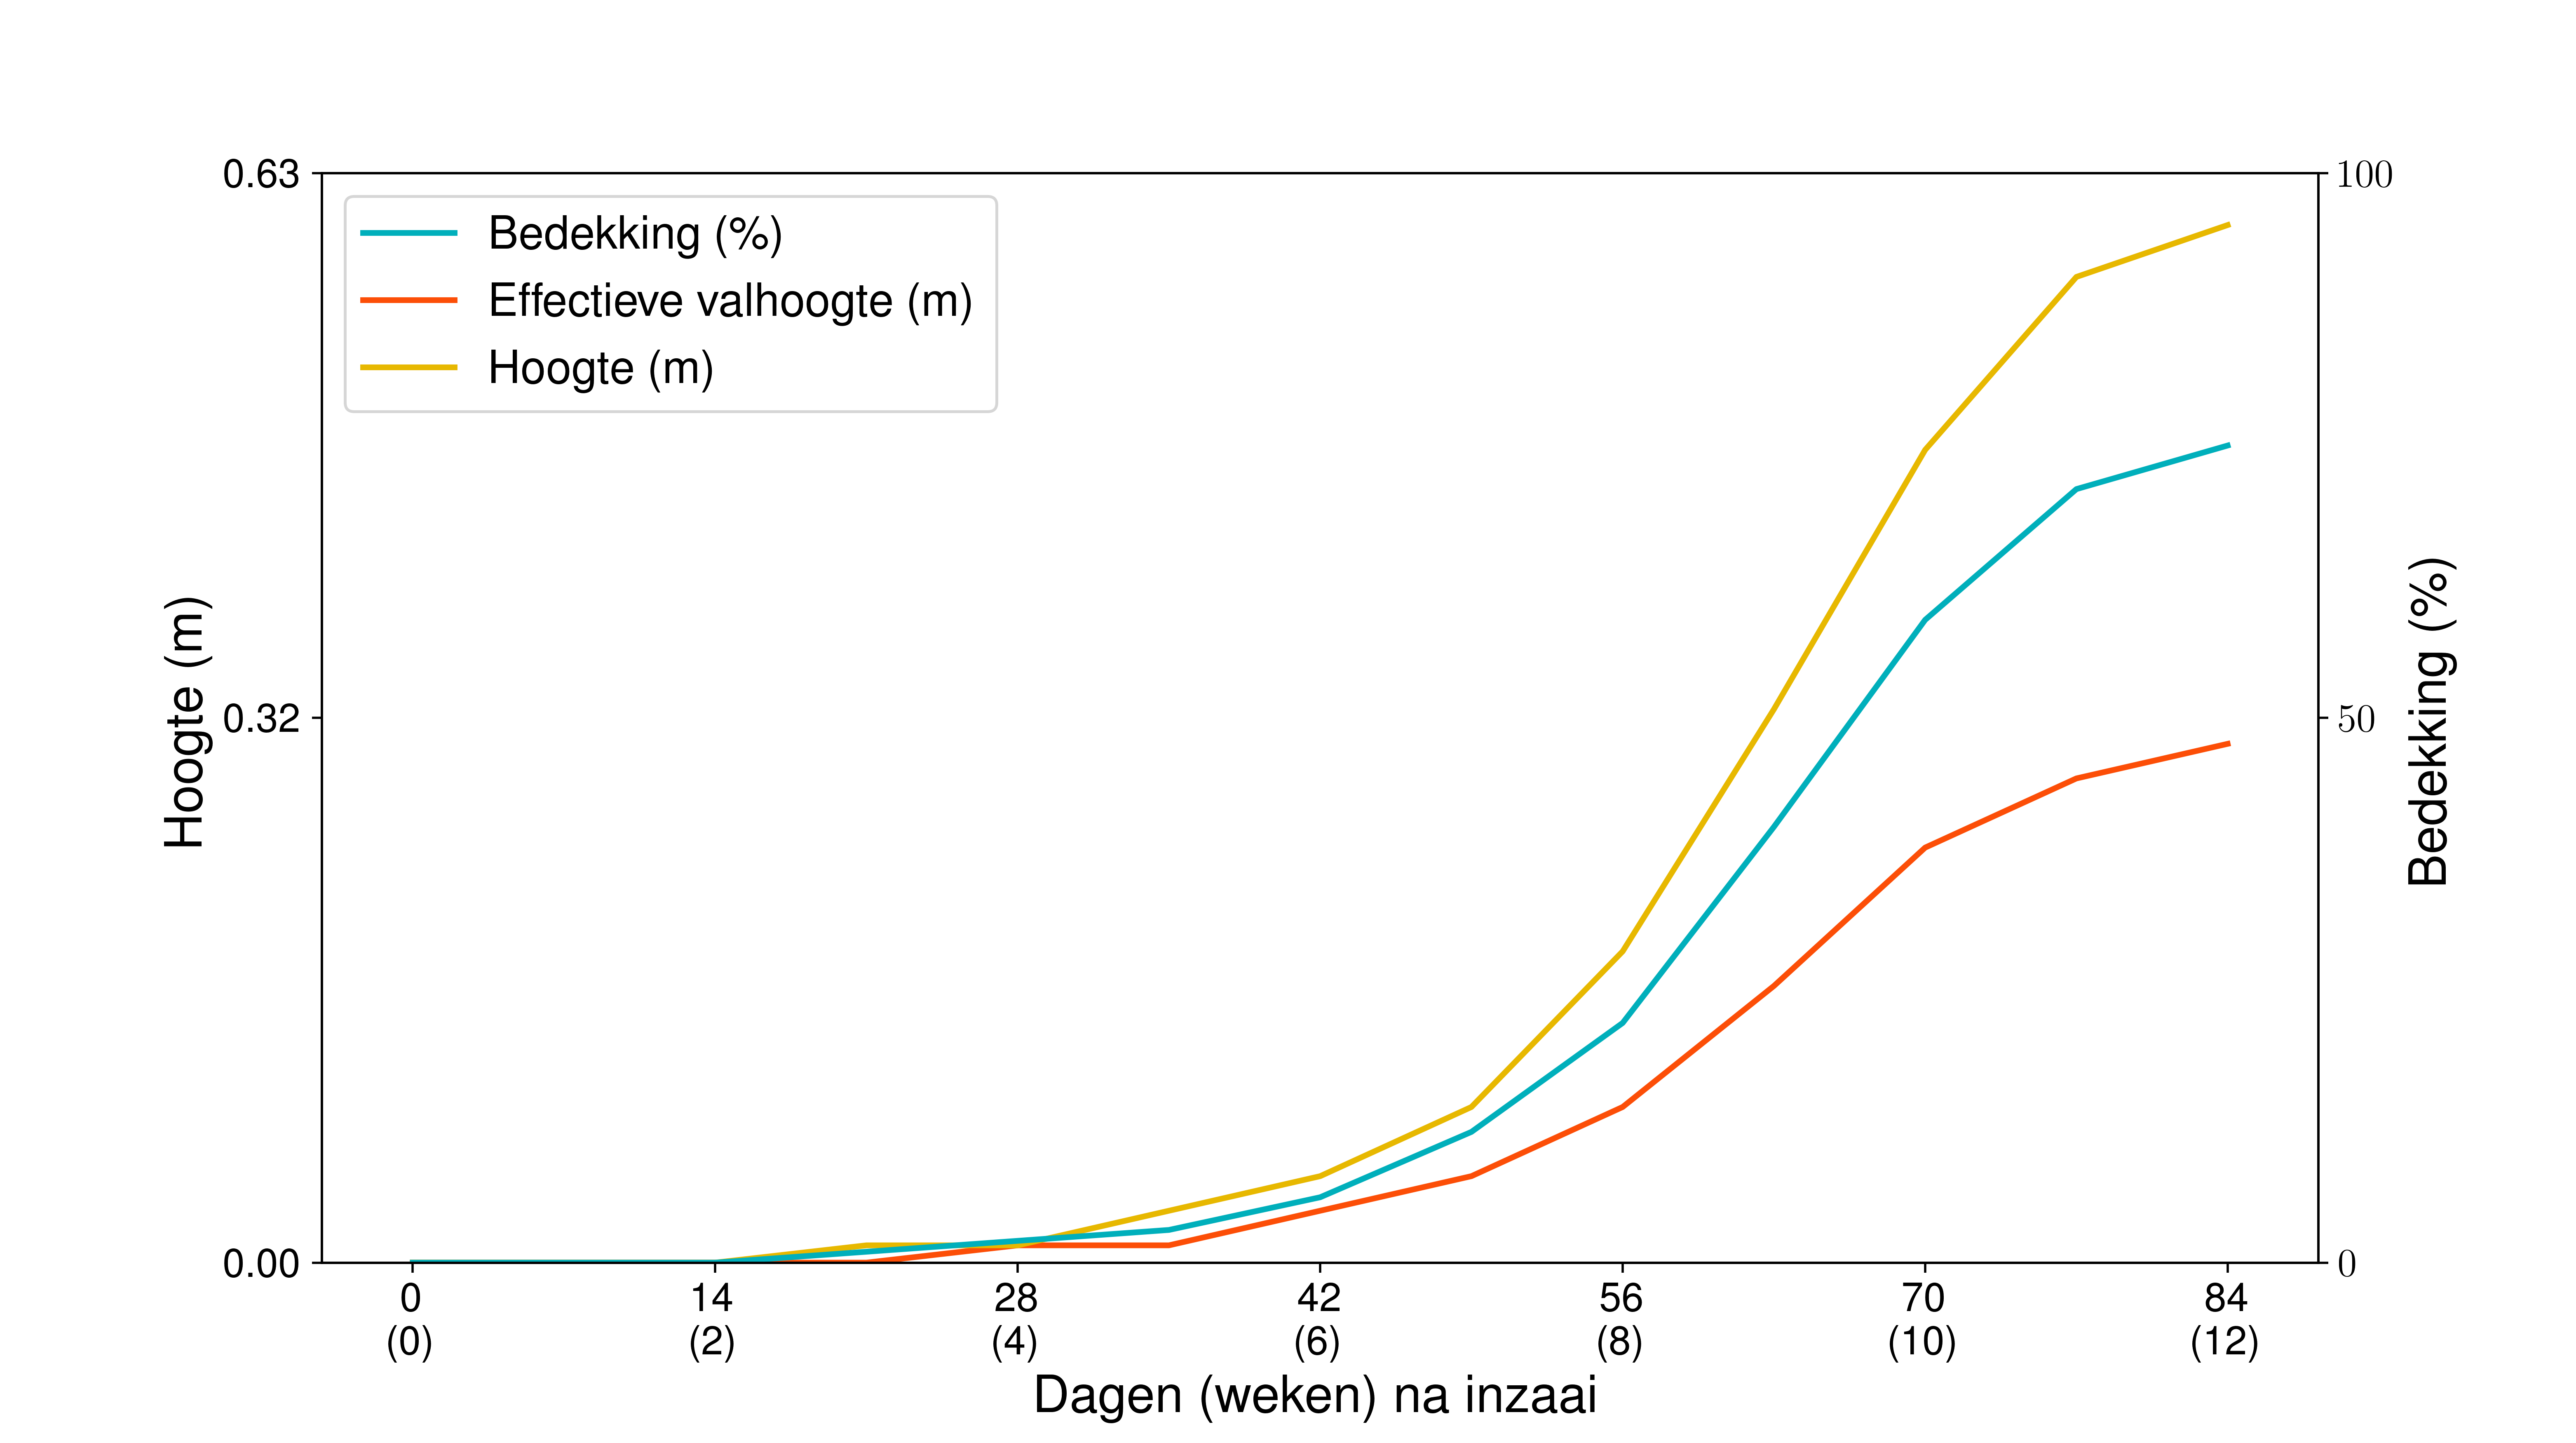
\includegraphics[width=12.5cm]{temp/1033.png} \end{figure} \end{center} 
  \textbf{Referenties:} Gabriels2003;ILVO2019;DeNeve2019 \vspace{0.10cm} \\ 
  \textbf{Opmerkingen?} verloop gewasgroeicurves geinterpoleerd met cumulatieve stikstofopname curve geraporteerd in Coopman et al. (2013) \vspace{0.10cm} \\ 
 \newpage 
 \subsection{Hoofdteelt (subgroep\_id 2033)} 
  \textbf{Zaaidatum (dd/mm)}: 15/06  \vspace{0.10cm} \\ 
  \textbf{Oogstdatum (dd/mm)}: 01/11  \vspace{0.10cm} \\ 
  \textbf{Oogstresten} \vspace{0.05cm} \\ 
  \tab Initi\"{e}le hoeveelheid (kg ha$^{-1}$): 3000.00 \vspace{0.05cm} \\ 
  \tab Afbraakcoefficient (-): 0.03 \vspace{0.05cm} \\ 
  \tab Bodembedekking (m$^2$ kg$^{-1}$): 1.07 \vspace{0.05cm} \\ 
  \tab Initieel percentage bedekking (\%): 28 \vspace{0.05cm} \\ 
  \tab Halfwaarde tijd (dagen): 10 \vspace{0.05cm} \\ 
  \textbf{Initi\"{e}le bodemruwheid (mm)}: 6.10 \vspace{0.05cm} \\ 
  \textbf{Gewasgroeicurve subgroep\_id 2033:} 
 \begin{center} \begin{figure}[H] 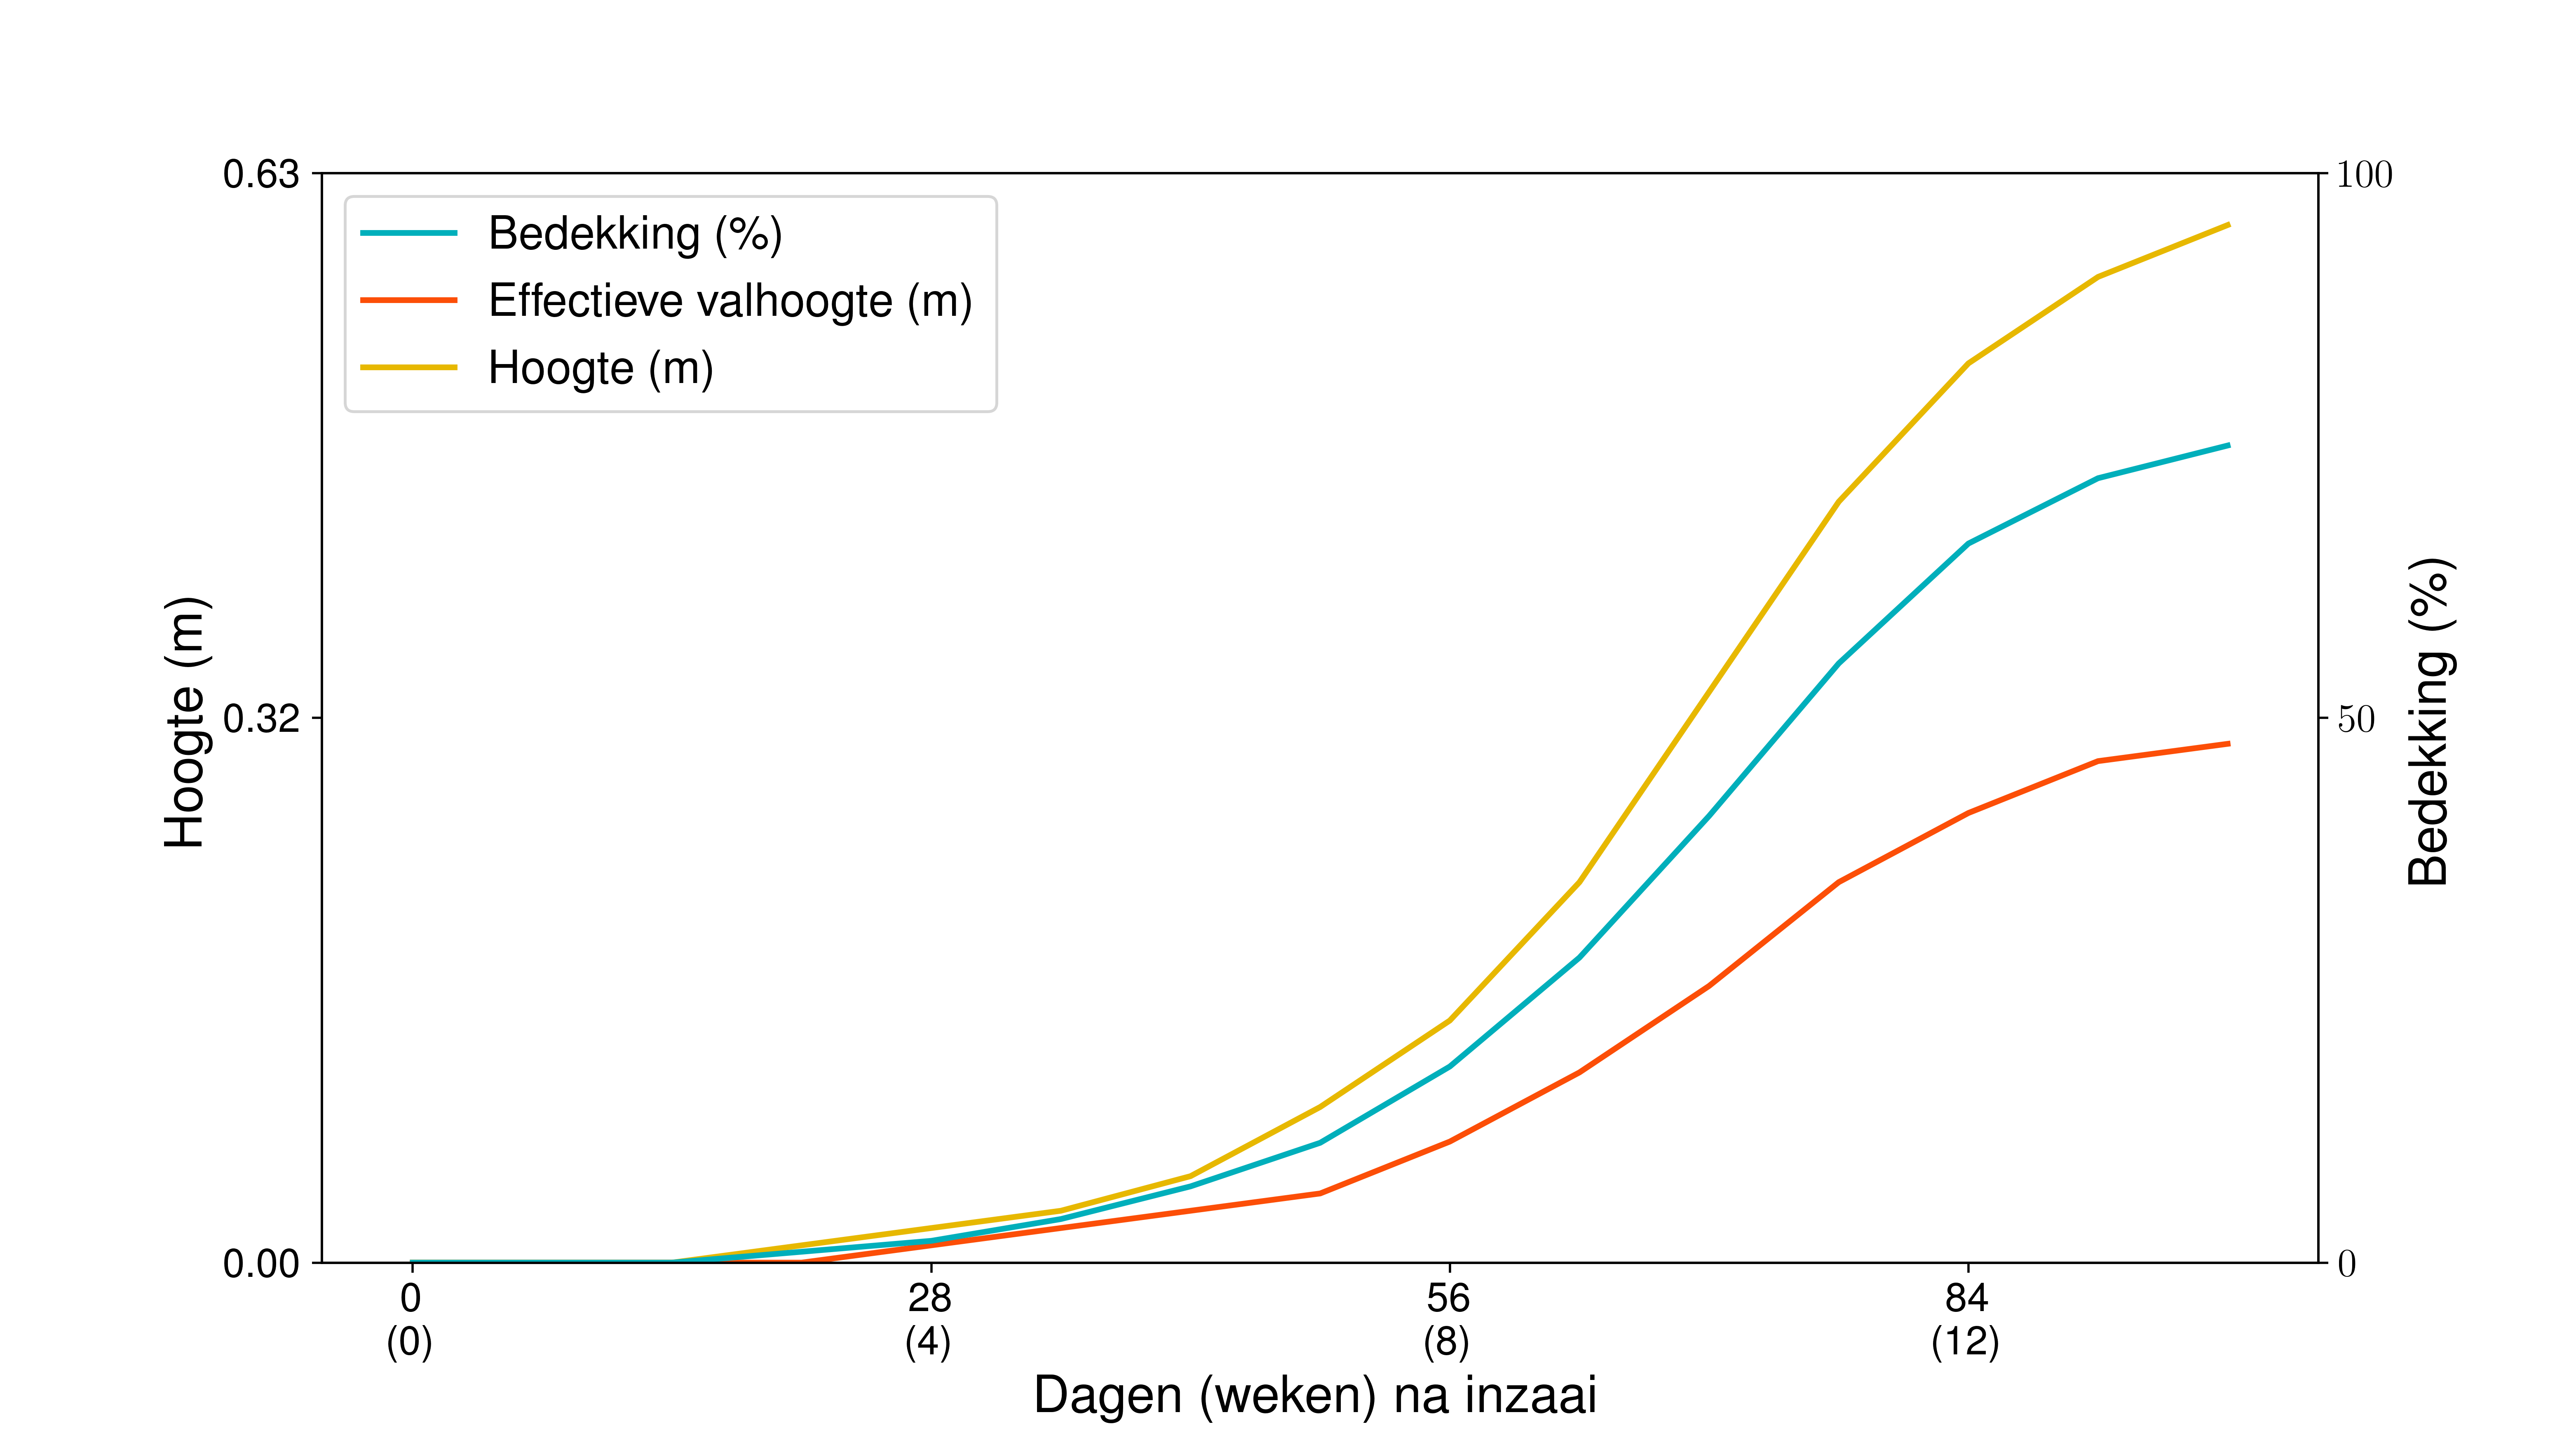
\includegraphics[width=12.5cm]{temp/2033.png} \end{figure} \end{center} 
  \textbf{Referenties:} Gabriels2003;ILVO2019;DeNeve2019 \vspace{0.10cm} \\ 
  \textbf{Opmerkingen?} verloop gewasgroeicurves geinterpoleerd met cumulatieve stikstofopname curve geraporteerd in Coopman et al. (2013) \vspace{0.10cm} \\ 
 \newpage 
 \subsection{Nateelt (subgroep\_id 3033)} 
  \textbf{Zaaidatum (dd/mm)}: 15/07  \vspace{0.10cm} \\ 
  \textbf{Oogstdatum (dd/mm)}: 15/01  \vspace{0.10cm} \\ 
  \textbf{Oogstresten} \vspace{0.05cm} \\ 
  \tab Initi\"{e}le hoeveelheid (kg ha$^{-1}$): 3000.00 \vspace{0.05cm} \\ 
  \tab Afbraakcoefficient (-): 0.03 \vspace{0.05cm} \\ 
  \tab Bodembedekking (m$^2$ kg$^{-1}$): 1.07 \vspace{0.05cm} \\ 
  \tab Initieel percentage bedekking (\%): 28 \vspace{0.05cm} \\ 
  \tab Halfwaarde tijd (dagen): 10 \vspace{0.05cm} \\ 
  \textbf{Initi\"{e}le bodemruwheid (mm)}: 6.10 \vspace{0.05cm} \\ 
  \textbf{Gewasgroeicurve subgroep\_id 3033:} 
 \begin{center} \begin{figure}[H] 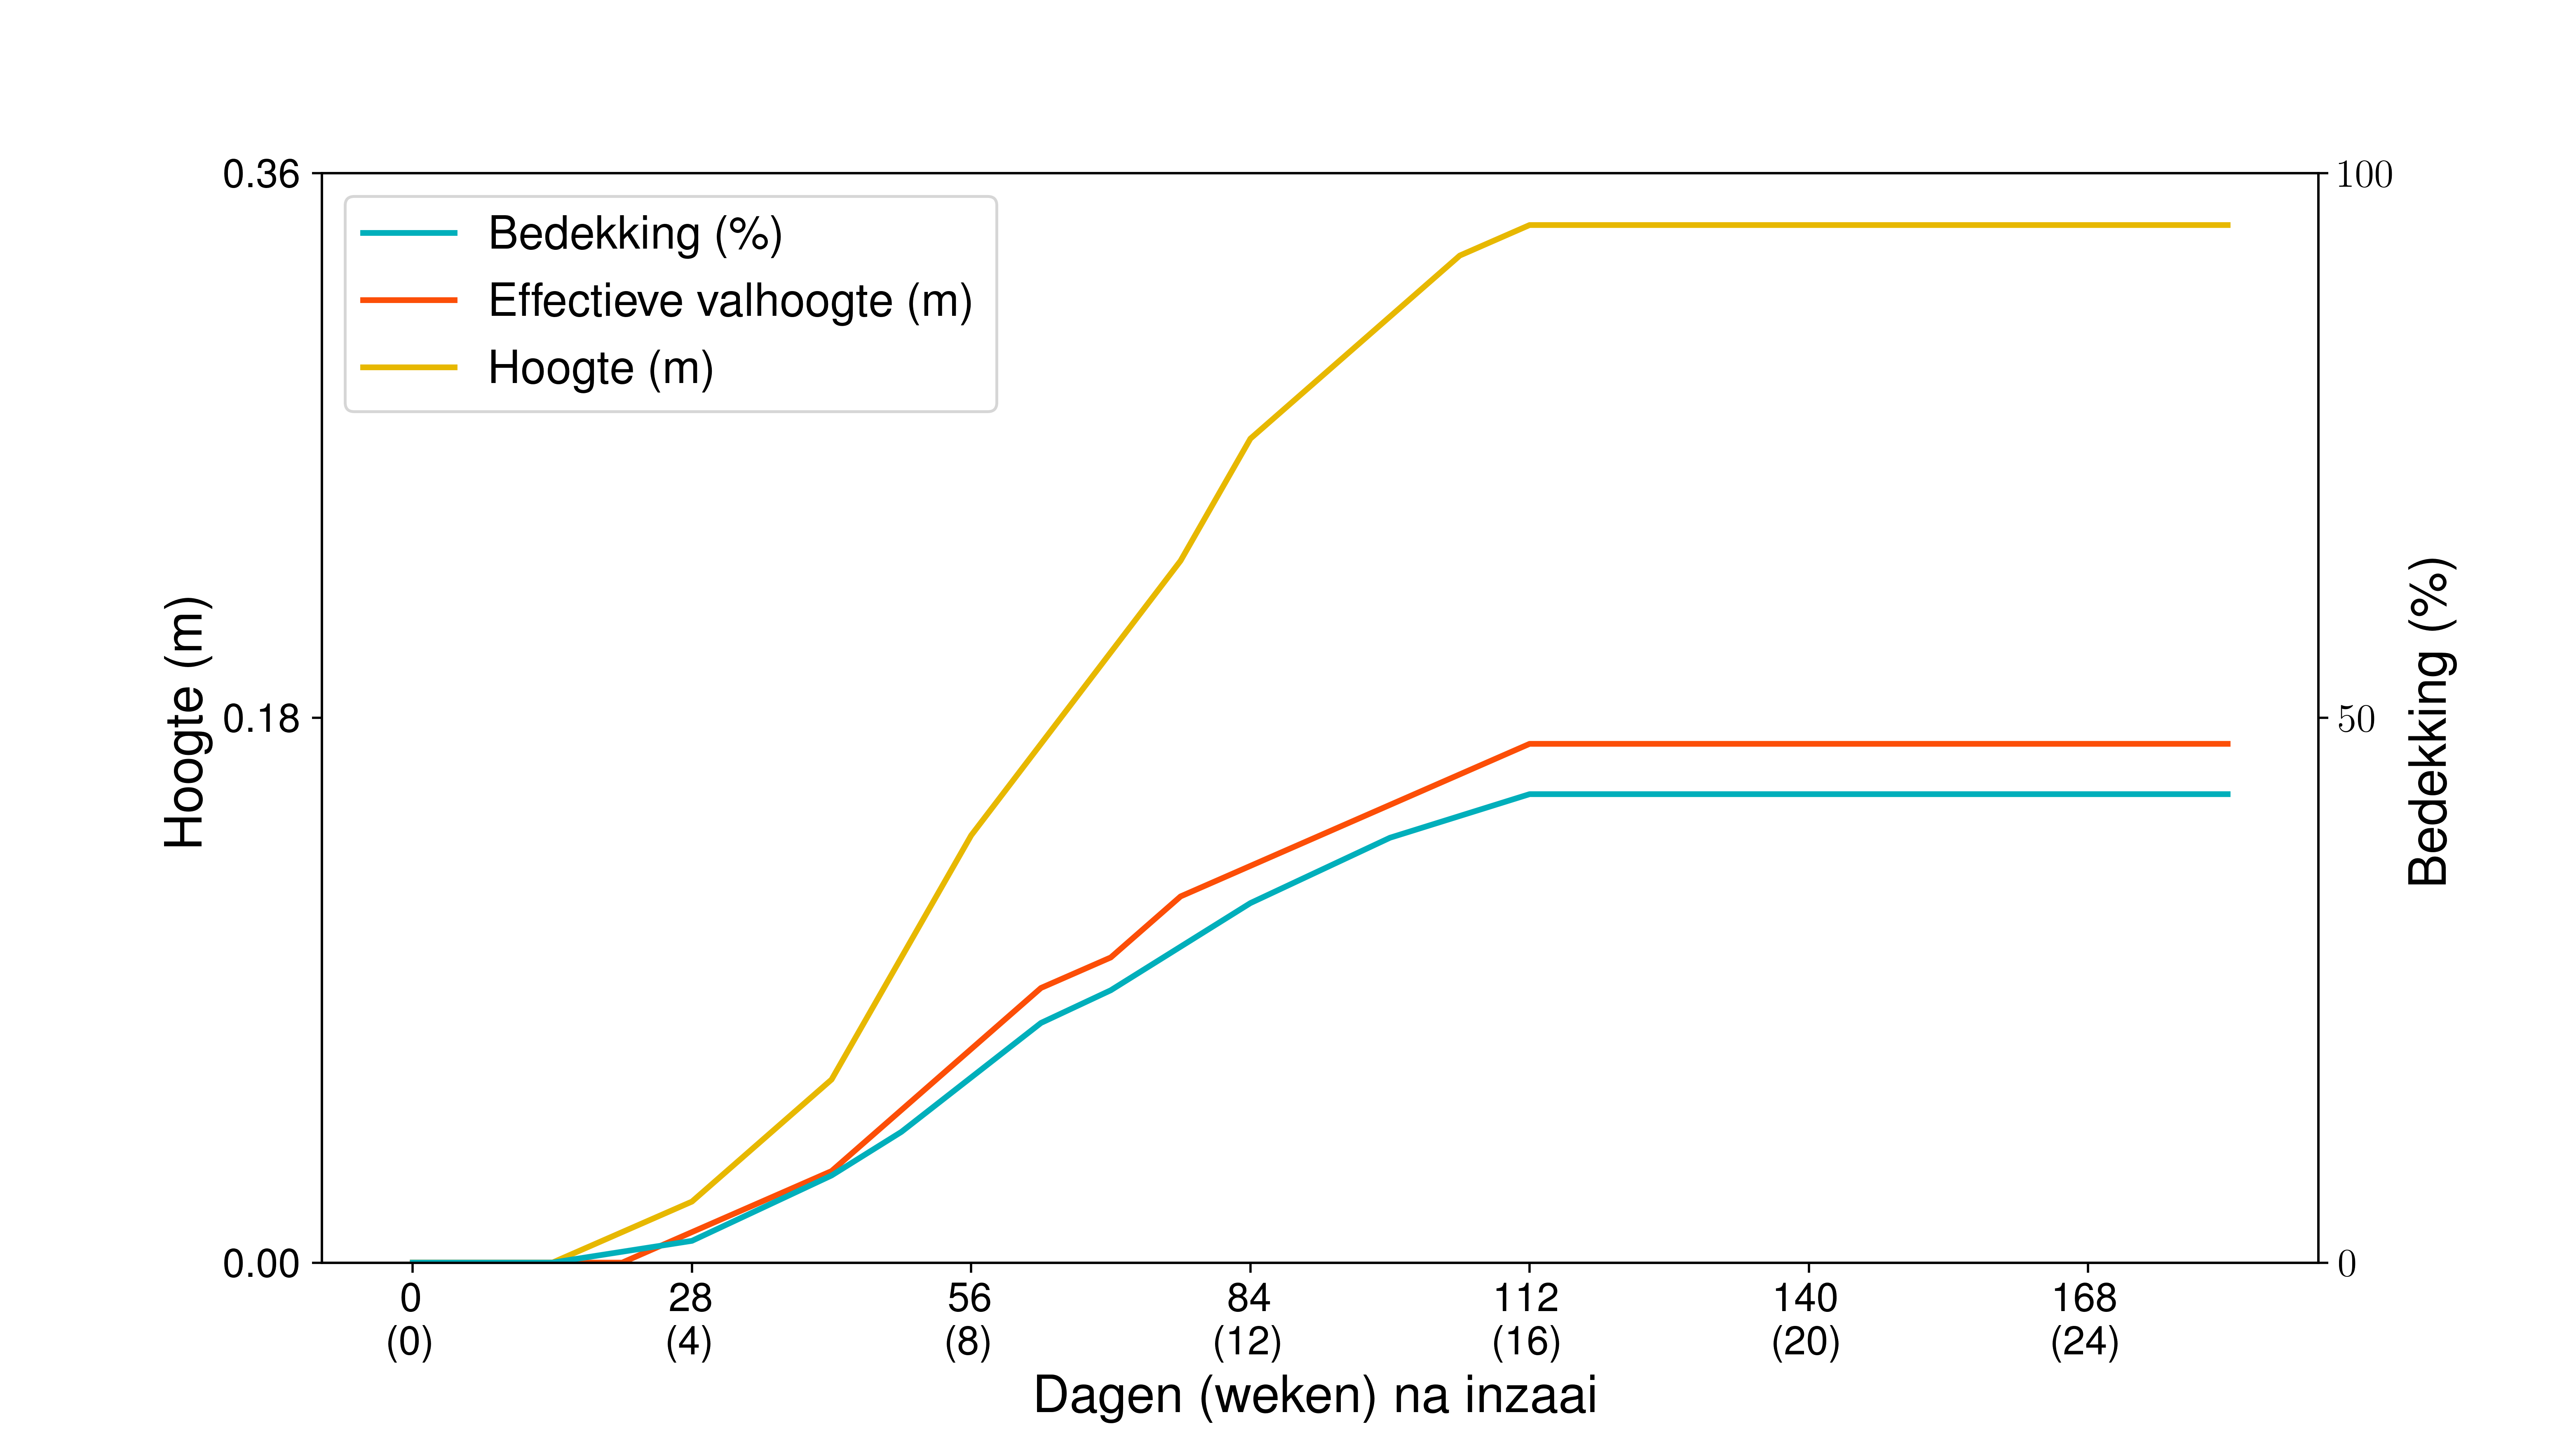
\includegraphics[width=12.5cm]{temp/3033.png} \end{figure} \end{center} 
  \textbf{Referenties:} Gabriels2003;ILVO2019;DeNeve2019 \vspace{0.10cm} \\ 
  \textbf{Opmerkingen?} verloop gewasgroeicurves geinterpoleerd met cumulatieve stikstofopname curve geraporteerd in Coopman et al. (2013) \vspace{0.10cm} \\ 
 \newpage 
 \section{Spinazie (groep\_id 34)} 
 \textbf{Van toepassing op gewasnamen (en codes):} Spinazie - industrie (8519) , Spinazie - vers (9519) 
 \begin{multicols}{3} \begin{itemize} \item[$\square$] Meerjarig \item[$\square$] Groenbedekker \item[$\boxtimes$] Groente \end{itemize} \end{multicols} 
 \subsection{Voorteelt (subgroep\_id 1034)} 
  \textbf{Zaaidatum (dd/mm)}: 01/04  \vspace{0.10cm} \\ 
  \textbf{Oogstdatum (dd/mm)}: 15/05  \vspace{0.10cm} \\ 
  \textbf{Oogstresten} \vspace{0.05cm} \\ 
  \tab Initi\"{e}le hoeveelheid (kg ha$^{-1}$): 0.00 \vspace{0.05cm} \\ 
  \tab Afbraakcoefficient (-): 0.00 \vspace{0.05cm} \\ 
  \tab Bodembedekking (m$^2$ kg$^{-1}$): 0.00 \vspace{0.05cm} \\ 
  \tab Initieel percentage bedekking (\%): 0 \vspace{0.05cm} \\ 
  \tab Halfwaarde tijd (dagen): 0 \vspace{0.05cm} \\ 
  \textbf{Initi\"{e}le bodemruwheid (mm)}: 7.60 \vspace{0.05cm} \\ 
  \textbf{Gewasgroeicurve subgroep\_id 1034:} 
 \begin{center} \begin{figure}[H] 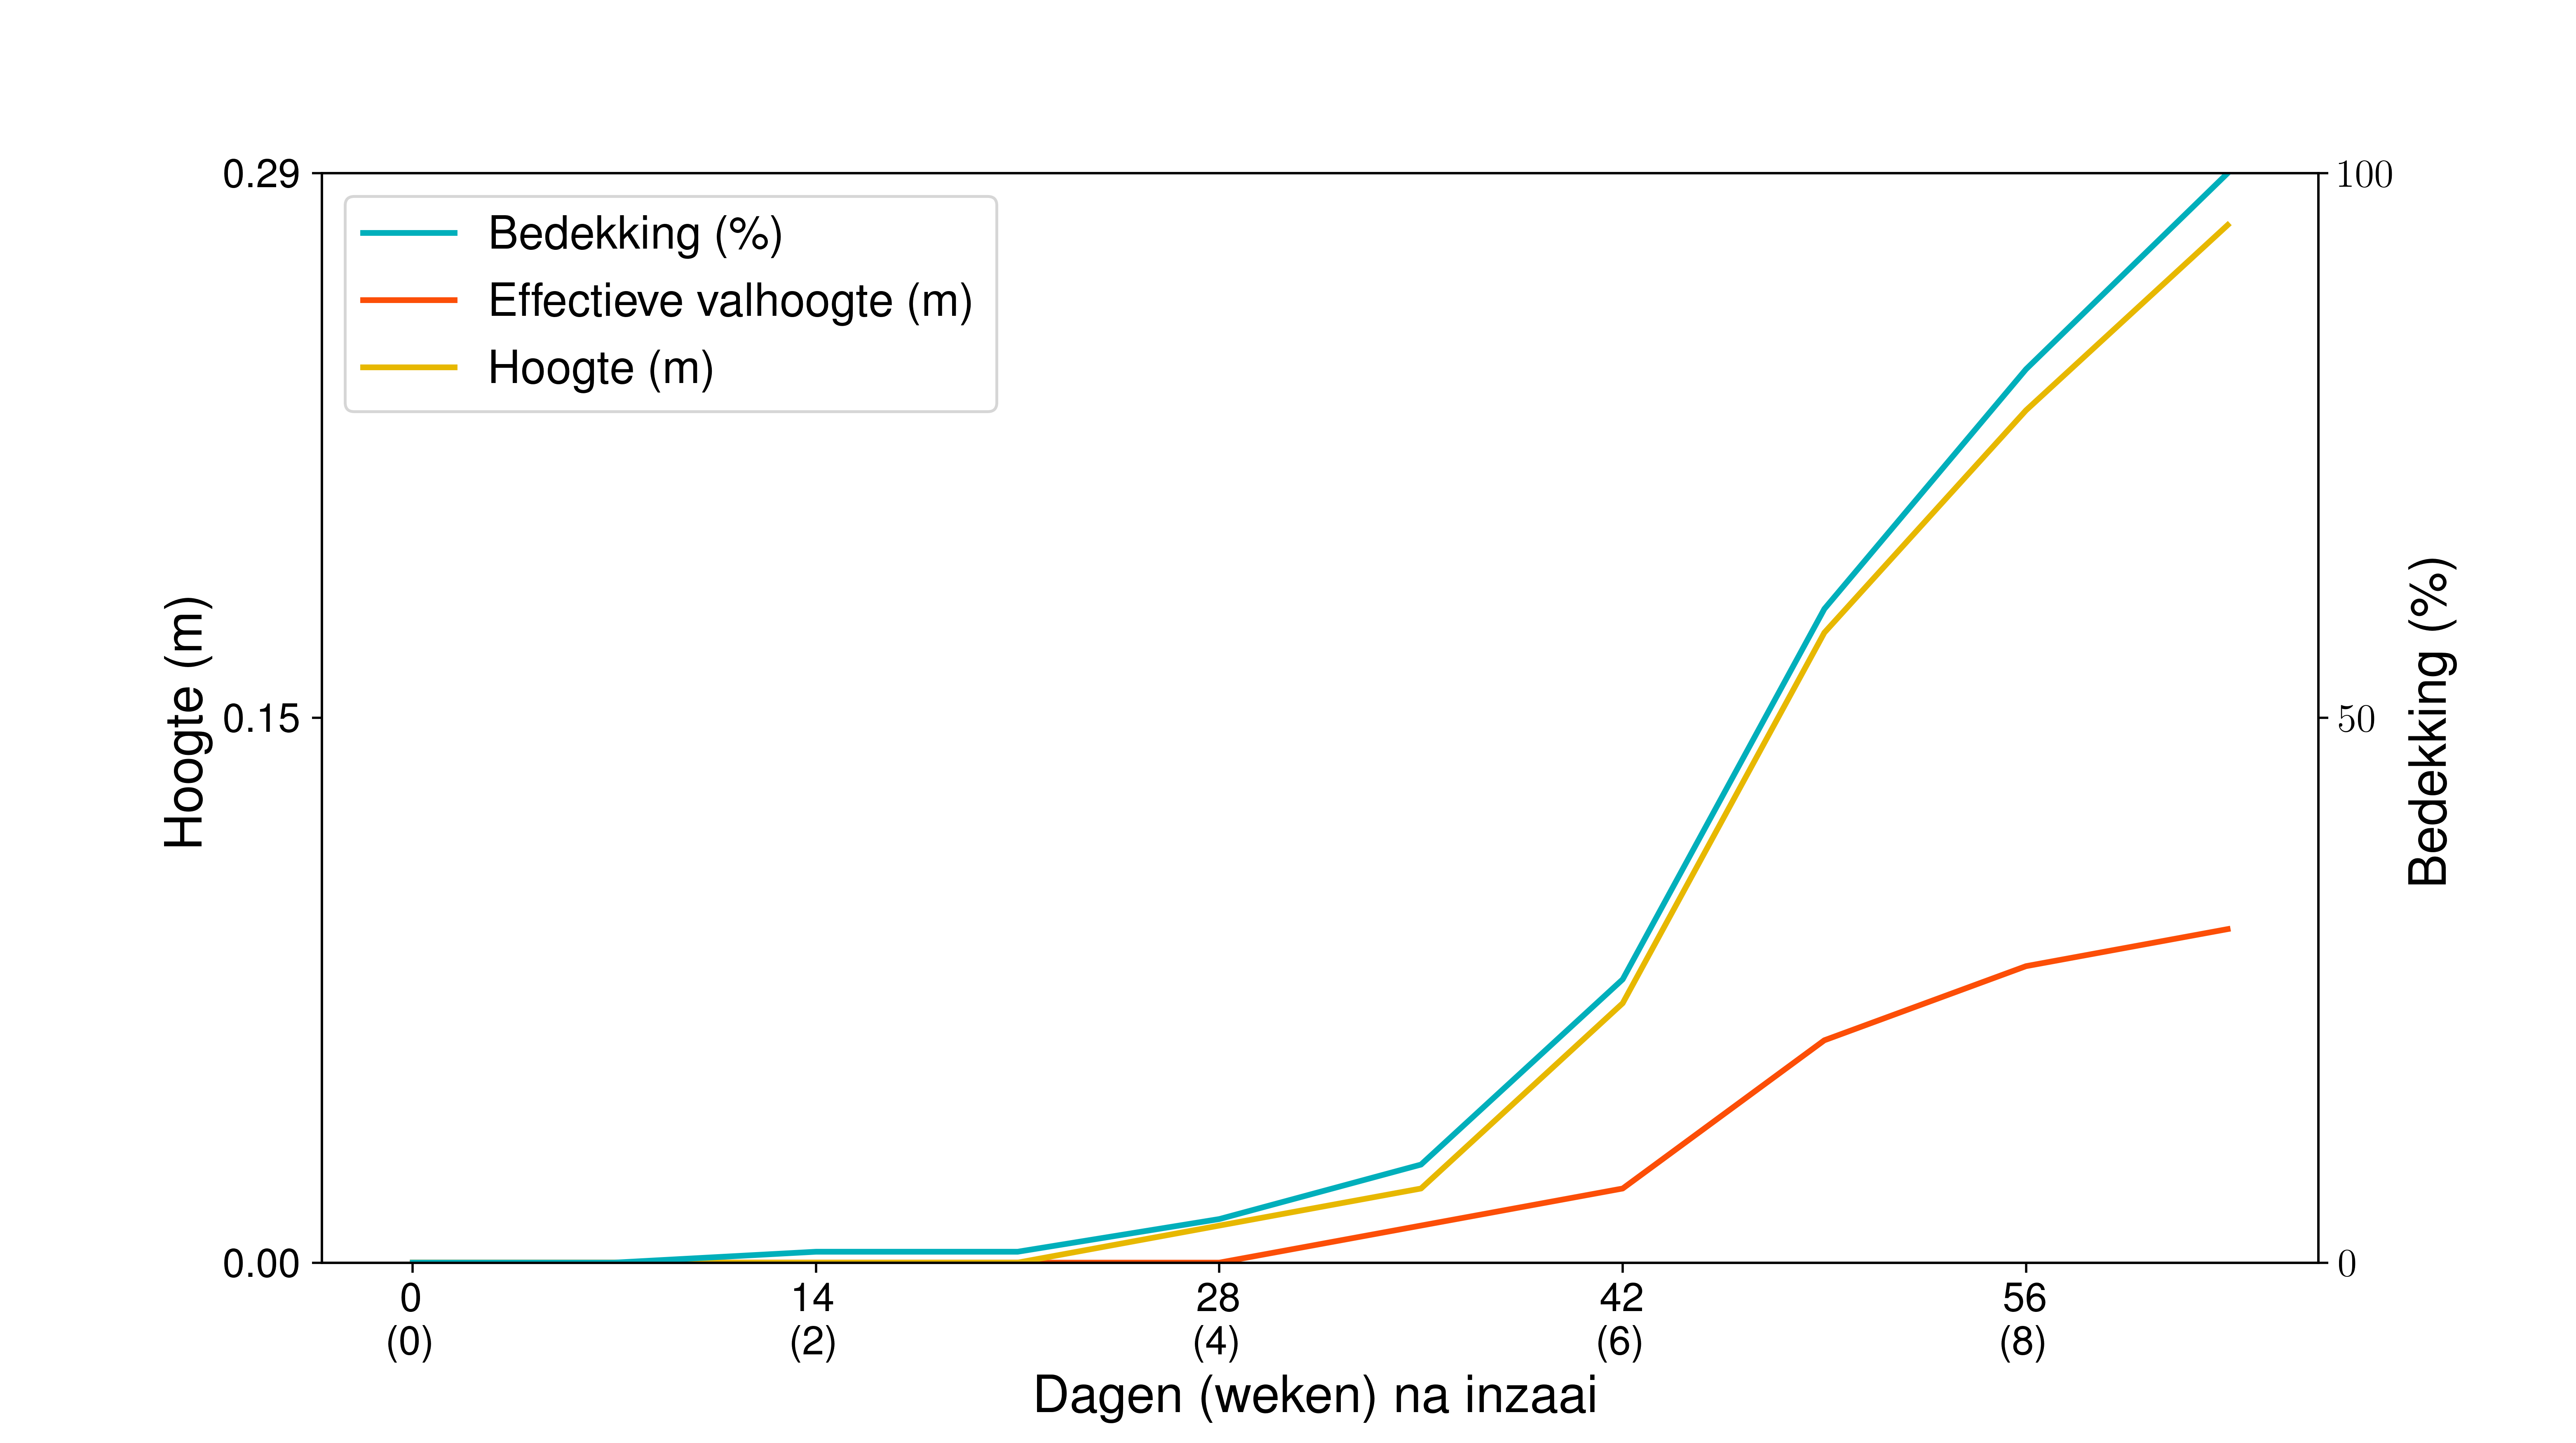
\includegraphics[width=12.5cm]{temp/1034.png} \end{figure} \end{center} 
  \textbf{Referenties:} ILVO2019 \vspace{0.10cm} \\ 
  \textbf{Opmerkingen?} geen \vspace{0.10cm} \\ 
 \newpage 
 \subsection{Hoofdteelt (subgroep\_id 2034)} 
  \textbf{Zaaidatum (dd/mm)}: 02/08  \vspace{0.10cm} \\ 
  \textbf{Oogstdatum (dd/mm)}: 12/10  \vspace{0.10cm} \\ 
  \textbf{Oogstresten} \vspace{0.05cm} \\ 
  \tab Initi\"{e}le hoeveelheid (kg ha$^{-1}$): 0.00 \vspace{0.05cm} \\ 
  \tab Afbraakcoefficient (-): 0.00 \vspace{0.05cm} \\ 
  \tab Bodembedekking (m$^2$ kg$^{-1}$): 0.00 \vspace{0.05cm} \\ 
  \tab Initieel percentage bedekking (\%): 0 \vspace{0.05cm} \\ 
  \tab Halfwaarde tijd (dagen): 0 \vspace{0.05cm} \\ 
  \textbf{Initi\"{e}le bodemruwheid (mm)}: 7.60 \vspace{0.05cm} \\ 
  \textbf{Gewasgroeicurve subgroep\_id 2034:} 
 \begin{center} \begin{figure}[H] 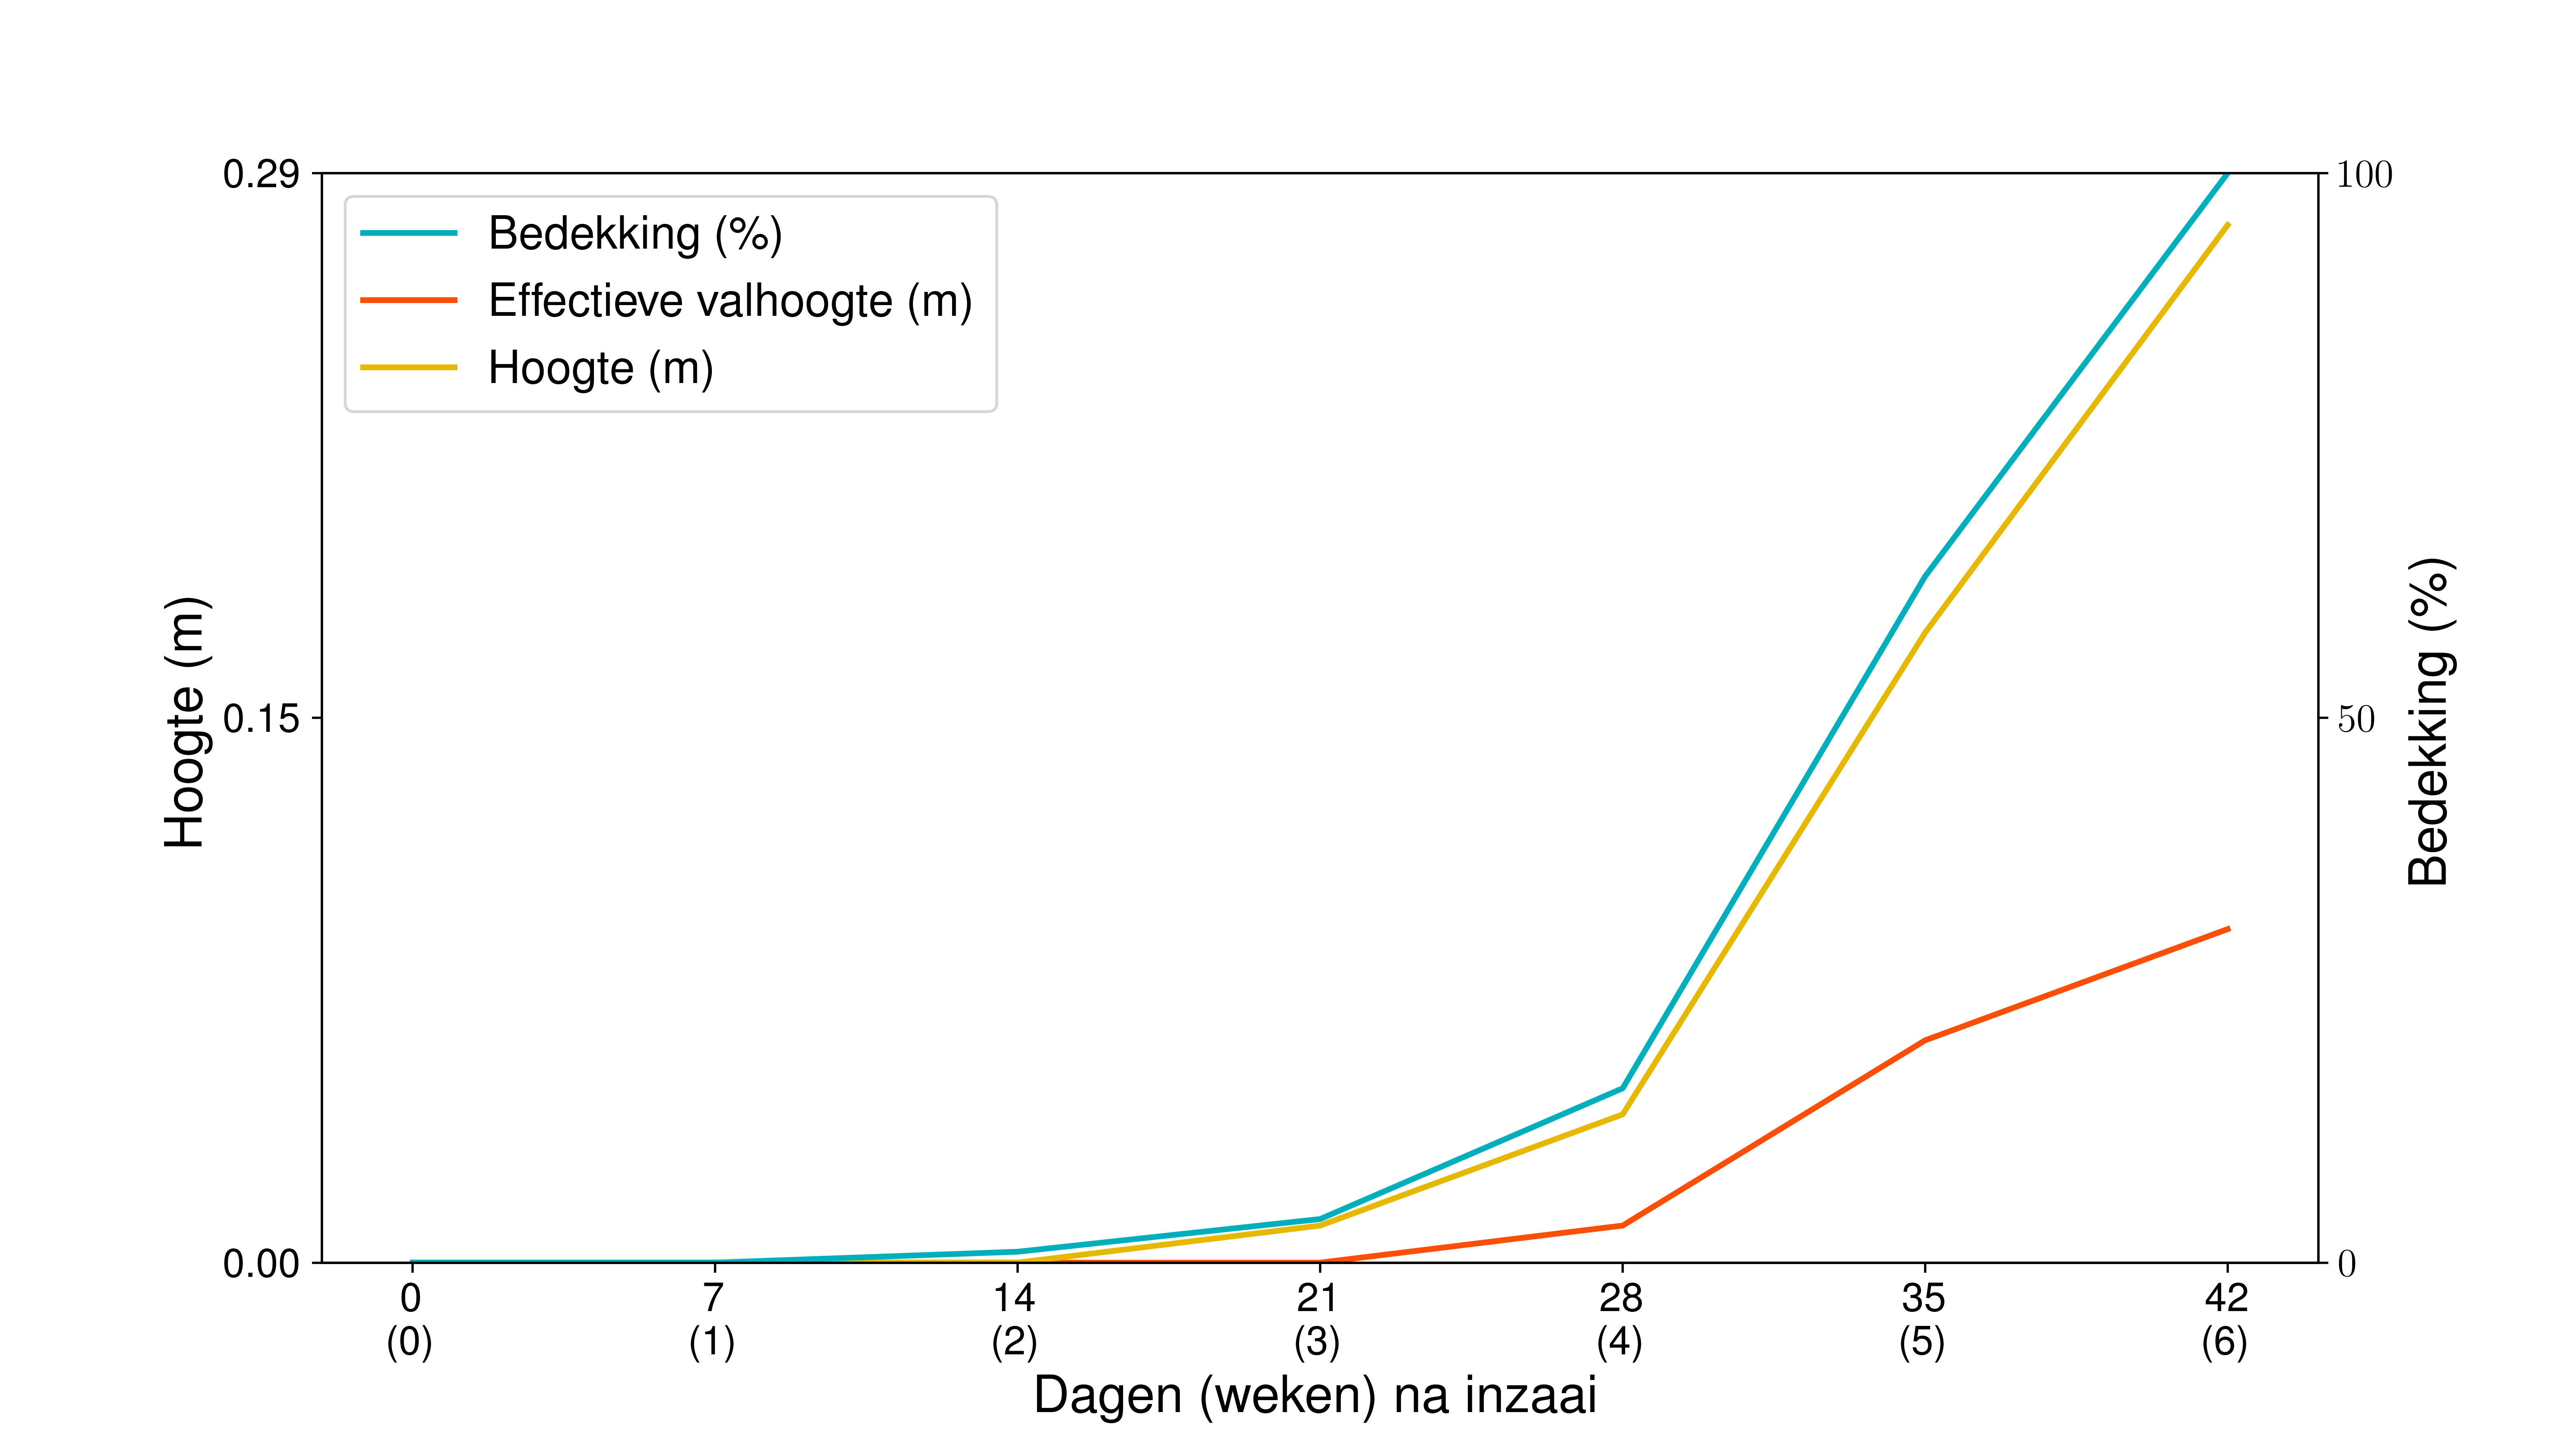
\includegraphics[width=12.5cm]{temp/2034.png} \end{figure} \end{center} 
  \textbf{Referenties:} ILVO2019 \vspace{0.10cm} \\ 
  \textbf{Opmerkingen?} geen \vspace{0.10cm} \\ 
 \newpage 
 \section{Bloemkool en broccoli - industrie (groep\_id 35)} 
 \textbf{Van toepassing op gewasnamen (en codes):} Bloemkool - industrie (8523) , Broccoli - industrie (8525) 
 \begin{multicols}{3} \begin{itemize} \item[$\square$] Meerjarig \item[$\square$] Groenbedekker \item[$\boxtimes$] Groente \end{itemize} \end{multicols} 
 \subsection{Voorteelt (subgroep\_id 1036)} 
  \textbf{Zaaidatum (dd/mm)}: 15/04  \vspace{0.10cm} \\ 
  \textbf{Oogstdatum (dd/mm)}: 01/07  \vspace{0.10cm} \\ 
  \textbf{Oogstresten} \vspace{0.05cm} \\ 
  \tab Initi\"{e}le hoeveelheid (kg ha$^{-1}$): 5000.00 \vspace{0.05cm} \\ 
  \tab Afbraakcoefficient (-): 0.05 \vspace{0.05cm} \\ 
  \tab Bodembedekking (m$^2$ kg$^{-1}$): 9.21 \vspace{0.05cm} \\ 
  \tab Initieel percentage bedekking (\%): 99 \vspace{0.05cm} \\ 
  \tab Halfwaarde tijd (dagen): 6 \vspace{0.05cm} \\ 
  \textbf{Initi\"{e}le bodemruwheid (mm)}: 10.20 \vspace{0.05cm} \\ 
  \textbf{Gewasgroeicurve subgroep\_id 1036:} 
 \begin{center} \begin{figure}[H] \includegraphics[width=12.5cm]{temp/1036.png} \end{figure} \end{center} 
  \textbf{Referenties:} ILVO2019;DeNeve2019 \vspace{0.10cm} \\ 
  \textbf{Opmerkingen?} geen \vspace{0.10cm} \\ 
 \newpage 
 \section{Bloemkool en broccoli - vers (groep\_id 36)} 
 \textbf{Van toepassing op gewasnamen (en codes):} Bloemkool - vers (9523) , Broccoli - vers (9525) 
 \begin{multicols}{3} \begin{itemize} \item[$\square$] Meerjarig \item[$\square$] Groenbedekker \item[$\boxtimes$] Groente \end{itemize} \end{multicols} 
  \textbf{Zaaidatum (dd/mm)}: 15/02  \vspace{0.10cm} \\ 
  \textbf{Oogstdatum (dd/mm)}: 15/12  \vspace{0.10cm} \\ 
  \textbf{Oogstresten} \vspace{0.05cm} \\ 
  \tab Initi\"{e}le hoeveelheid (kg ha$^{-1}$): 5000.00 \vspace{0.05cm} \\ 
  \tab Afbraakcoefficient (-): 0.05 \vspace{0.05cm} \\ 
  \tab Bodembedekking (m$^2$ kg$^{-1}$): 9.21 \vspace{0.05cm} \\ 
  \tab Initieel percentage bedekking (\%): 99 \vspace{0.05cm} \\ 
  \tab Halfwaarde tijd (dagen): 6 \vspace{0.05cm} \\ 
  \textbf{Initi\"{e}le bodemruwheid (mm)}: 10.20 \vspace{0.05cm} \\ 
  \textbf{Gewasgroeicurve subgroep\_id 1036:} 
 \begin{center} \begin{figure}[H] \includegraphics[width=12.5cm]{temp/1036.png} \end{figure} \end{center} 
  \textbf{Referenties:} ILVO2019;DeNeve2019 \vspace{0.10cm} \\ 
  \textbf{Opmerkingen?} geen \vspace{0.10cm} \\ 
 \newpage 
 \section{Spruitkool - industrie (groep\_id 37)} 
 \textbf{Van toepassing op gewasnamen (en codes):} Spruitkool - industrie (8512) 
 \begin{multicols}{3} \begin{itemize} \item[$\square$] Meerjarig \item[$\square$] Groenbedekker \item[$\boxtimes$] Groente \end{itemize} \end{multicols} 
  \textbf{Zaaidatum (dd/mm)}: 01/05  \vspace{0.10cm} \\ 
  \textbf{Oogstdatum (dd/mm)}: 01/12  \vspace{0.10cm} \\ 
  \textbf{Oogstresten} \vspace{0.05cm} \\ 
  \tab Initi\"{e}le hoeveelheid (kg ha$^{-1}$): 8000.00 \vspace{0.05cm} \\ 
  \tab Afbraakcoefficient (-): 0.05 \vspace{0.05cm} \\ 
  \tab Bodembedekking (m$^2$ kg$^{-1}$): 5.76 \vspace{0.05cm} \\ 
  \tab Initieel percentage bedekking (\%): 99 \vspace{0.05cm} \\ 
  \tab Halfwaarde tijd (dagen): 6 \vspace{0.05cm} \\ 
  \textbf{Initi\"{e}le bodemruwheid (mm)}: 10.20 \vspace{0.05cm} \\ 
  \textbf{Gewasgroeicurve subgroep\_id 1037:} 
 \begin{center} \begin{figure}[H] \includegraphics[width=12.5cm]{temp/1037.png} \end{figure} \end{center} 
  \textbf{Referenties:} ILVO2019 \vspace{0.10cm} \\ 
  \textbf{Opmerkingen?} geen \vspace{0.10cm} \\ 
 \newpage 
 \section{Spruitkolen - vers (groep\_id 38)} 
 \textbf{Van toepassing op gewasnamen (en codes):} Spruitkolen - vers (9512) 
 \begin{multicols}{3} \begin{itemize} \item[$\square$] Meerjarig \item[$\square$] Groenbedekker \item[$\boxtimes$] Groente \end{itemize} \end{multicols} 
  \textbf{Zaaidatum (dd/mm)}: 01/05  \vspace{0.10cm} \\ 
  \textbf{Oogstdatum (dd/mm)}: 01/12  \vspace{0.10cm} \\ 
  \textbf{Oogstresten} \vspace{0.05cm} \\ 
  \tab Initi\"{e}le hoeveelheid (kg ha$^{-1}$): 8000.00 \vspace{0.05cm} \\ 
  \tab Afbraakcoefficient (-): 0.05 \vspace{0.05cm} \\ 
  \tab Bodembedekking (m$^2$ kg$^{-1}$): 5.76 \vspace{0.05cm} \\ 
  \tab Initieel percentage bedekking (\%): 99 \vspace{0.05cm} \\ 
  \tab Halfwaarde tijd (dagen): 6 \vspace{0.05cm} \\ 
  \textbf{Initi\"{e}le bodemruwheid (mm)}: 10.20 \vspace{0.05cm} \\ 
  \textbf{Gewasgroeicurve subgroep\_id 1037:} 
 \begin{center} \begin{figure}[H] \includegraphics[width=12.5cm]{temp/1037.png} \end{figure} \end{center} 
  \textbf{Referenties:} ILVO2019 \vspace{0.10cm} \\ 
  \textbf{Opmerkingen?} geen \vspace{0.10cm} \\ 
 \newpage 
 \section{Kolen - industrie (groep\_id 39)} 
 \textbf{Van toepassing op gewasnamen (en codes):} Witte kool - industrie (8540) , Rode kool - industrie (8527) , Savooikool - industrie (8546) 
 \begin{multicols}{3} \begin{itemize} \item[$\square$] Meerjarig \item[$\square$] Groenbedekker \item[$\boxtimes$] Groente \end{itemize} \end{multicols} 
  \textbf{Zaaidatum (dd/mm)}: 15/05  \vspace{0.10cm} \\ 
  \textbf{Oogstdatum (dd/mm)}: 15/10  \vspace{0.10cm} \\ 
  \textbf{Oogstresten} \vspace{0.05cm} \\ 
  \tab Initi\"{e}le hoeveelheid (kg ha$^{-1}$): 7000.00 \vspace{0.05cm} \\ 
  \tab Afbraakcoefficient (-): 0.05 \vspace{0.05cm} \\ 
  \tab Bodembedekking (m$^2$ kg$^{-1}$): 6.58 \vspace{0.05cm} \\ 
  \tab Initieel percentage bedekking (\%): 99 \vspace{0.05cm} \\ 
  \tab Halfwaarde tijd (dagen): 6 \vspace{0.05cm} \\ 
  \textbf{Initi\"{e}le bodemruwheid (mm)}: 10.20 \vspace{0.05cm} \\ 
  \textbf{Gewasgroeicurve subgroep\_id 1039:} 
 \begin{center} \begin{figure}[H] \includegraphics[width=12.5cm]{temp/1039.png} \end{figure} \end{center} 
  \textbf{Referenties:} ILVO2019 \vspace{0.10cm} \\ 
  \textbf{Opmerkingen?} geen \vspace{0.10cm} \\ 
 \newpage 
 \section{Kolen - vers (groep\_id 40)} 
 \textbf{Van toepassing op gewasnamen (en codes):} Witte kool - vers (9540) , Rode kool - vers (9527) , Savooikool - vers (9546) 
 \begin{multicols}{3} \begin{itemize} \item[$\square$] Meerjarig \item[$\square$] Groenbedekker \item[$\boxtimes$] Groente \end{itemize} \end{multicols} 
  \textbf{Zaaidatum (dd/mm)}: 01/06  \vspace{0.10cm} \\ 
  \textbf{Oogstdatum (dd/mm)}: 15/10  \vspace{0.10cm} \\ 
  \textbf{Oogstresten} \vspace{0.05cm} \\ 
  \tab Initi\"{e}le hoeveelheid (kg ha$^{-1}$): 7000.00 \vspace{0.05cm} \\ 
  \tab Afbraakcoefficient (-): 0.05 \vspace{0.05cm} \\ 
  \tab Bodembedekking (m$^2$ kg$^{-1}$): 6.58 \vspace{0.05cm} \\ 
  \tab Initieel percentage bedekking (\%): 99 \vspace{0.05cm} \\ 
  \tab Halfwaarde tijd (dagen): 6 \vspace{0.05cm} \\ 
  \textbf{Initi\"{e}le bodemruwheid (mm)}: 10.20 \vspace{0.05cm} \\ 
  \textbf{Gewasgroeicurve subgroep\_id 1040:} 
 \begin{center} \begin{figure}[H] \includegraphics[width=12.5cm]{temp/1040.png} \end{figure} \end{center} 
  \textbf{Referenties:} ILVO2019 \vspace{0.10cm} \\ 
  \textbf{Opmerkingen?} geen \vspace{0.10cm} \\ 
 \newpage 
 \section{Knolselder - industrie (groep\_id 41)} 
 \textbf{Van toepassing op gewasnamen (en codes):} Knolselder - industrie (8543) 
 \begin{multicols}{3} \begin{itemize} \item[$\square$] Meerjarig \item[$\square$] Groenbedekker \item[$\boxtimes$] Groente \end{itemize} \end{multicols} 
  \textbf{Zaaidatum (dd/mm)}: 01/05  \vspace{0.10cm} \\ 
  \textbf{Oogstdatum (dd/mm)}: 01/12  \vspace{0.10cm} \\ 
  \textbf{Oogstresten} \vspace{0.05cm} \\ 
  \tab Initi\"{e}le hoeveelheid (kg ha$^{-1}$): 3000.00 \vspace{0.05cm} \\ 
  \tab Afbraakcoefficient (-): 0.05 \vspace{0.05cm} \\ 
  \tab Bodembedekking (m$^2$ kg$^{-1}$): 15.35 \vspace{0.05cm} \\ 
  \tab Initieel percentage bedekking (\%): 80 \vspace{0.05cm} \\ 
  \tab Halfwaarde tijd (dagen): 6 \vspace{0.05cm} \\ 
  \textbf{Initi\"{e}le bodemruwheid (mm)}: 10.20 \vspace{0.05cm} \\ 
  \textbf{Gewasgroeicurve subgroep\_id 1041:} 
 \begin{center} \begin{figure}[H] \includegraphics[width=12.5cm]{temp/1041.png} \end{figure} \end{center} 
  \textbf{Referenties:} ILVO2019 \vspace{0.10cm} \\ 
  \textbf{Opmerkingen?} verloop gewasgroeicurves geinterpoleerd met cumulatieve stikstofopname curve geraporteerd in Coopman et al. (2013) \vspace{0.10cm} \\ 
 \newpage 
 \section{Knolselder - vers (groep\_id 42)} 
 \textbf{Van toepassing op gewasnamen (en codes):} Knolselder - vers (9543) 
 \begin{multicols}{3} \begin{itemize} \item[$\square$] Meerjarig \item[$\square$] Groenbedekker \item[$\boxtimes$] Groente \end{itemize} \end{multicols} 
  \textbf{Zaaidatum (dd/mm)}: 01/03  \vspace{0.10cm} \\ 
  \textbf{Oogstdatum (dd/mm)}: 01/07  \vspace{0.10cm} \\ 
  \textbf{Oogstresten} \vspace{0.05cm} \\ 
  \tab Initi\"{e}le hoeveelheid (kg ha$^{-1}$): 3000.00 \vspace{0.05cm} \\ 
  \tab Afbraakcoefficient (-): 0.05 \vspace{0.05cm} \\ 
  \tab Bodembedekking (m$^2$ kg$^{-1}$): 15.35 \vspace{0.05cm} \\ 
  \tab Initieel percentage bedekking (\%): 80 \vspace{0.05cm} \\ 
  \tab Halfwaarde tijd (dagen): 6 \vspace{0.05cm} \\ 
  \textbf{Initi\"{e}le bodemruwheid (mm)}: 10.20 \vspace{0.05cm} \\ 
  \textbf{Gewasgroeicurve subgroep\_id 1041:} 
 \begin{center} \begin{figure}[H] \includegraphics[width=12.5cm]{temp/1041.png} \end{figure} \end{center} 
  \textbf{Referenties:} ILVO2019  \vspace{0.10cm} \\ 
  \textbf{Opmerkingen?} verloop gewasgroeicurves geinterpoleerd met cumulatieve stikstofopname curve geraporteerd in Coopman et al. (2013) \vspace{0.10cm} \\ 
 \newpage 
 \section{Pastinaak  (groep\_id 43)} 
 \textbf{Van toepassing op gewasnamen (en codes):} Pastinaak - industrie (8409) , Pastinaak - vers (9409) 
 \begin{multicols}{3} \begin{itemize} \item[$\square$] Meerjarig \item[$\square$] Groenbedekker \item[$\boxtimes$] Groente \end{itemize} \end{multicols} 
  \textbf{Zaaidatum (dd/mm)}: 01/05  \vspace{0.10cm} \\ 
  \textbf{Oogstdatum (dd/mm)}: 15/02  \vspace{0.10cm} \\ 
  \textbf{Oogstresten} \vspace{0.05cm} \\ 
  \tab Initi\"{e}le hoeveelheid (kg ha$^{-1}$): 0.00 \vspace{0.05cm} \\ 
  \tab Afbraakcoefficient (-): 0.00 \vspace{0.05cm} \\ 
  \tab Bodembedekking (m$^2$ kg$^{-1}$): 0.00 \vspace{0.05cm} \\ 
  \tab Initieel percentage bedekking (\%): 0 \vspace{0.05cm} \\ 
  \tab Halfwaarde tijd (dagen): 0 \vspace{0.05cm} \\ 
  \textbf{Initi\"{e}le bodemruwheid (mm)}: 6.10 \vspace{0.05cm} \\ 
  \textbf{Gewasgroeicurve subgroep\_id 1043:} 
 \begin{center} \begin{figure}[H] \includegraphics[width=12.5cm]{temp/1043.png} \end{figure} \end{center} 
  \textbf{Referenties:} ILVO2019 \vspace{0.10cm} \\ 
  \textbf{Opmerkingen?} geen \vspace{0.10cm} \\ 
 \newpage 
 \section{Schorseneer (groep\_id 44)} 
 \textbf{Van toepassing op gewasnamen (en codes):} Schorseneer - industrie (8533) , Schorseneer - vers (9533) 
 \begin{multicols}{3} \begin{itemize} \item[$\square$] Meerjarig \item[$\square$] Groenbedekker \item[$\boxtimes$] Groente \end{itemize} \end{multicols} 
  \textbf{Zaaidatum (dd/mm)}: 01/05  \vspace{0.10cm} \\ 
  \textbf{Oogstdatum (dd/mm)}: 15/02  \vspace{0.10cm} \\ 
  \textbf{Oogstresten} \vspace{0.05cm} \\ 
  \tab Initi\"{e}le hoeveelheid (kg ha$^{-1}$): 0.00 \vspace{0.05cm} \\ 
  \tab Afbraakcoefficient (-): 0.00 \vspace{0.05cm} \\ 
  \tab Bodembedekking (m$^2$ kg$^{-1}$): 0.00 \vspace{0.05cm} \\ 
  \tab Initieel percentage bedekking (\%): 0 \vspace{0.05cm} \\ 
  \tab Halfwaarde tijd (dagen): 0 \vspace{0.05cm} \\ 
  \textbf{Initi\"{e}le bodemruwheid (mm)}: 6.10 \vspace{0.05cm} \\ 
  \textbf{Gewasgroeicurve subgroep\_id 1044:} 
 \begin{center} \begin{figure}[H] \includegraphics[width=12.5cm]{temp/1044.png} \end{figure} \end{center} 
  \textbf{Referenties:} ILVO2019 \vspace{0.10cm} \\ 
  \textbf{Opmerkingen?} geen \vspace{0.10cm} \\ 
 \newpage 
 \section{Kropsla (groep\_id 45)} 
 \textbf{Van toepassing op gewasnamen (en codes):} Kropsla - industrie (8518) , Kropsla - vers (9518) 
 \begin{multicols}{3} \begin{itemize} \item[$\square$] Meerjarig \item[$\square$] Groenbedekker \item[$\boxtimes$] Groente \end{itemize} \end{multicols} 
  \textbf{Zaaidatum (dd/mm)}: 01/05  \vspace{0.10cm} \\ 
  \textbf{Oogstdatum (dd/mm)}: 15/09  \vspace{0.10cm} \\ 
  \textbf{Oogstresten} \vspace{0.05cm} \\ 
  \tab Initi\"{e}le hoeveelheid (kg ha$^{-1}$): 1500.00 \vspace{0.05cm} \\ 
  \tab Afbraakcoefficient (-): 0.00 \vspace{0.05cm} \\ 
  \tab Bodembedekking (m$^2$ kg$^{-1}$): 0.00 \vspace{0.05cm} \\ 
  \tab Initieel percentage bedekking (\%): 0 \vspace{0.05cm} \\ 
  \tab Halfwaarde tijd (dagen): 0 \vspace{0.05cm} \\ 
  \textbf{Initi\"{e}le bodemruwheid (mm)}: 7.60 \vspace{0.05cm} \\ 
  \textbf{Gewasgroeicurve subgroep\_id 1045:} 
 \begin{center} \begin{figure}[H] \includegraphics[width=12.5cm]{temp/1045.png} \end{figure} \end{center} 
  \textbf{Referenties:} ILVO2019 \vspace{0.10cm} \\ 
  \textbf{Opmerkingen?} verloop gewasgroeicurves geinterpoleerd met cumulatieve stikstofopname curve geraporteerd in Coopman et al. (2013) \vspace{0.10cm} \\ 
 \newpage 
 \section{Asperge (groep\_id 46)} 
 \textbf{Van toepassing op gewasnamen (en codes):} Asperge - industrie (8511) , Asperge - vers (9511) 
 \begin{multicols}{3} \begin{itemize} \item[$\square$] Meerjarig \item[$\square$] Groenbedekker \item[$\boxtimes$] Groente \end{itemize} \end{multicols} 
  \textbf{Zaaidatum (dd/mm)}: 15/06  \vspace{0.10cm} \\ 
  \textbf{Oogstdatum (dd/mm)}: 15/11  \vspace{0.10cm} \\ 
  \textbf{Oogstresten} \vspace{0.05cm} \\ 
  \tab Initi\"{e}le hoeveelheid (kg ha$^{-1}$): 0.00 \vspace{0.05cm} \\ 
  \tab Afbraakcoefficient (-): 0.00 \vspace{0.05cm} \\ 
  \tab Bodembedekking (m$^2$ kg$^{-1}$): 0.00 \vspace{0.05cm} \\ 
  \tab Initieel percentage bedekking (\%): 0 \vspace{0.05cm} \\ 
  \tab Halfwaarde tijd (dagen): 0 \vspace{0.05cm} \\ 
  \textbf{Initi\"{e}le bodemruwheid (mm)}: 7.60 \vspace{0.05cm} \\ 
  \textbf{Gewasgroeicurve subgroep\_id 1046:} 
 \begin{center} \begin{figure}[H] \includegraphics[width=12.5cm]{temp/1046.png} \end{figure} \end{center} 
  \textbf{Referenties:} ILVO2019 \vspace{0.10cm} \\ 
  \textbf{Opmerkingen?} geen \vspace{0.10cm} \\ 
 \newpage 
 \section{Courgettes - industrie (groep\_id 47)} 
 \textbf{Van toepassing op gewasnamen (en codes):} Courgettes - industrie (8541) 
 \begin{multicols}{3} \begin{itemize} \item[$\square$] Meerjarig \item[$\square$] Groenbedekker \item[$\boxtimes$] Groente \end{itemize} \end{multicols} 
  \textbf{Zaaidatum (dd/mm)}: 01/06  \vspace{0.10cm} \\ 
  \textbf{Oogstdatum (dd/mm)}: 01/10  \vspace{0.10cm} \\ 
  \textbf{Oogstresten} \vspace{0.05cm} \\ 
  \tab Initi\"{e}le hoeveelheid (kg ha$^{-1}$): 0.00 \vspace{0.05cm} \\ 
  \tab Afbraakcoefficient (-): 0.00 \vspace{0.05cm} \\ 
  \tab Bodembedekking (m$^2$ kg$^{-1}$): 0.00 \vspace{0.05cm} \\ 
  \tab Initieel percentage bedekking (\%): 0 \vspace{0.05cm} \\ 
  \tab Halfwaarde tijd (dagen): 0 \vspace{0.05cm} \\ 
  \textbf{Initi\"{e}le bodemruwheid (mm)}: 7.60 \vspace{0.05cm} \\ 
  \textbf{Gewasgroeicurve subgroep\_id 1047:} 
 \begin{center} \begin{figure}[H] \includegraphics[width=12.5cm]{temp/1047.png} \end{figure} \end{center} 
  \textbf{Referenties:} ILVO2019 \vspace{0.10cm} \\ 
  \textbf{Opmerkingen?} geen \vspace{0.10cm} \\ 
 \newpage 
 \section{Courgettes - vers (groep\_id 48)} 
 \textbf{Van toepassing op gewasnamen (en codes):} Courgettes - vers (9541) 
 \begin{multicols}{3} \begin{itemize} \item[$\square$] Meerjarig \item[$\square$] Groenbedekker \item[$\boxtimes$] Groente \end{itemize} \end{multicols} 
 \subsection{Voorteelt (subgroep\_id 1048)} 
  \textbf{Zaaidatum (dd/mm)}: 01/05  \vspace{0.10cm} \\ 
  \textbf{Oogstdatum (dd/mm)}: 15/09  \vspace{0.10cm} \\ 
  \textbf{Oogstresten} \vspace{0.05cm} \\ 
  \tab Initi\"{e}le hoeveelheid (kg ha$^{-1}$): 0.00 \vspace{0.05cm} \\ 
  \tab Afbraakcoefficient (-): 0.00 \vspace{0.05cm} \\ 
  \tab Bodembedekking (m$^2$ kg$^{-1}$): 0.00 \vspace{0.05cm} \\ 
  \tab Initieel percentage bedekking (\%): 0 \vspace{0.05cm} \\ 
  \tab Halfwaarde tijd (dagen): 0 \vspace{0.05cm} \\ 
  \textbf{Initi\"{e}le bodemruwheid (mm)}: 7.60 \vspace{0.05cm} \\ 
  \textbf{Gewasgroeicurve subgroep\_id 1048:} 
 \begin{center} \begin{figure}[H] \includegraphics[width=12.5cm]{temp/1048.png} \end{figure} \end{center} 
  \textbf{Referenties:} ILVO2019 \vspace{0.10cm} \\ 
  \textbf{Opmerkingen?} geen \vspace{0.10cm} \\ 
 \newpage 
 \section{Stamslabonen (groep\_id 49)} 
 \textbf{Van toepassing op gewasnamen (en codes):} Stamslabonen - industrie (8410) , Stamslabonen - vers (9410) 
 \begin{multicols}{3} \begin{itemize} \item[$\square$] Meerjarig \item[$\square$] Groenbedekker \item[$\boxtimes$] Groente \end{itemize} \end{multicols} 
  \textbf{Zaaidatum (dd/mm)}: 15/06  \vspace{0.10cm} \\ 
  \textbf{Oogstdatum (dd/mm)}: 01/09  \vspace{0.10cm} \\ 
  \textbf{Oogstresten} \vspace{0.05cm} \\ 
  \tab Initi\"{e}le hoeveelheid (kg ha$^{-1}$): 5000.00 \vspace{0.05cm} \\ 
  \tab Afbraakcoefficient (-): / \vspace{0.05cm} \\ 
  \tab Bodembedekking (m$^2$ kg$^{-1}$): 9.21 \vspace{0.05cm} \\ 
  \tab Initieel percentage bedekking (\%): 99 \vspace{0.05cm} \\ 
  \tab Halfwaarde tijd (dagen): / \vspace{0.05cm} \\ 
  \textbf{Initi\"{e}le bodemruwheid (mm)}: 7.60 \vspace{0.05cm} \\ 
  \textbf{Gewasgroeicurve subgroep\_id 1049:} 
 \begin{center} \begin{figure}[H] \includegraphics[width=12.5cm]{temp/1049.png} \end{figure} \end{center} 
  \textbf{Referenties:} ILVO2019 \vspace{0.10cm} \\ 
  \textbf{Opmerkingen?} geen \vspace{0.10cm} \\ 
 \newpage 
 \section{Tuin- en veldbonen (groep\_id 50)} 
 \textbf{Van toepassing op gewasnamen (en codes):} Tuin- en veldbonen (Vicia faba) - vers (832) , Tuin- en veldbonen (Vicia faba) - industrie (932) , Tuin- en veldbonen (droog geoogst) (52) 
 \begin{multicols}{3} \begin{itemize} \item[$\square$] Meerjarig \item[$\square$] Groenbedekker \item[$\boxtimes$] Groente \end{itemize} \end{multicols} 
 \subsection{Voorteelt (subgroep\_id 1050)} 
  \textbf{Zaaidatum (dd/mm)}: 25/03  \vspace{0.10cm} \\ 
  \textbf{Oogstdatum (dd/mm)}: 01/09  \vspace{0.10cm} \\ 
  \textbf{Oogstresten} \vspace{0.05cm} \\ 
  \tab Initi\"{e}le hoeveelheid (kg ha$^{-1}$): 2000.00 \vspace{0.05cm} \\ 
  \tab Afbraakcoefficient (-): 0.01 \vspace{0.05cm} \\ 
  \tab Bodembedekking (m$^2$ kg$^{-1}$): 23.03 \vspace{0.05cm} \\ 
  \tab Initieel percentage bedekking (\%): 99 \vspace{0.05cm} \\ 
  \tab Halfwaarde tijd (dagen): 30 \vspace{0.05cm} \\ 
  \textbf{Initi\"{e}le bodemruwheid (mm)}: 10.20 \vspace{0.05cm} \\ 
  \textbf{Gewasgroeicurve subgroep\_id 1050:} 
 \begin{center} \begin{figure}[H] \includegraphics[width=12.5cm]{temp/1050.png} \end{figure} \end{center} 
  \textbf{Referenties:} ILVO2019 \vspace{0.10cm} \\ 
  \textbf{Opmerkingen?} geen \vspace{0.10cm} \\ 
 \newpage 
 \subsection{Nateelt (subgroep\_id 2050)} 
  \textbf{Zaaidatum (dd/mm)}: 01/11  \vspace{0.10cm} \\ 
  \textbf{Oogstdatum (dd/mm)}: 01/08  \vspace{0.10cm} \\ 
  \textbf{Oogstresten} \vspace{0.05cm} \\ 
  \tab Initi\"{e}le hoeveelheid (kg ha$^{-1}$): 2000.00 \vspace{0.05cm} \\ 
  \tab Afbraakcoefficient (-): 0.01 \vspace{0.05cm} \\ 
  \tab Bodembedekking (m$^2$ kg$^{-1}$): 23.03 \vspace{0.05cm} \\ 
  \tab Initieel percentage bedekking (\%): 99 \vspace{0.05cm} \\ 
  \tab Halfwaarde tijd (dagen): 30 \vspace{0.05cm} \\ 
  \textbf{Initi\"{e}le bodemruwheid (mm)}: 10.20 \vspace{0.05cm} \\ 
  \textbf{Gewasgroeicurve subgroep\_id 2050:} 
 \begin{center} \begin{figure}[H] \includegraphics[width=12.5cm]{temp/2050.png} \end{figure} \end{center} 
  \textbf{Referenties:} ILVO2019 \vspace{0.10cm} \\ 
  \textbf{Opmerkingen?} geen \vspace{0.10cm} \\ 
 \newpage 
 \section{Voedererwten (groep\_id 51)} 
 \textbf{Van toepassing op gewasnamen (en codes):} Voedererwten (niet voor menselijke consumptie) (51) 
 \begin{multicols}{3} \begin{itemize} \item[$\square$] Meerjarig \item[$\square$] Groenbedekker \item[$\boxtimes$] Groente \end{itemize} \end{multicols} 
  \textbf{Zaaidatum (dd/mm)}: 01/04  \vspace{0.10cm} \\ 
  \textbf{Oogstdatum (dd/mm)}: 01/08  \vspace{0.10cm} \\ 
  \textbf{Oogstresten} \vspace{0.05cm} \\ 
  \tab Initi\"{e}le hoeveelheid (kg ha$^{-1}$): 0.00 \vspace{0.05cm} \\ 
  \tab Afbraakcoefficient (-): 0.00 \vspace{0.05cm} \\ 
  \tab Bodembedekking (m$^2$ kg$^{-1}$): 0.00 \vspace{0.05cm} \\ 
  \tab Initieel percentage bedekking (\%): 0 \vspace{0.05cm} \\ 
  \tab Halfwaarde tijd (dagen): 0 \vspace{0.05cm} \\ 
  \textbf{Initi\"{e}le bodemruwheid (mm)}: 10.20 \vspace{0.05cm} \\ 
  \textbf{Gewasgroeicurve subgroep\_id 1051:} 
 \begin{center} \begin{figure}[H] \includegraphics[width=12.5cm]{temp/1051.png} \end{figure} \end{center} 
  \textbf{Referenties:} ILVO2019 \vspace{0.10cm} \\ 
  \textbf{Opmerkingen?} geen \vspace{0.10cm} \\ 
 \newpage 
 \section{Erwten (groep\_id 52)} 
 \textbf{Van toepassing op gewasnamen (en codes):} Erwten (andere dan droog geoogst) - industrie (831) , Erwten (andere dan droog geoogst) - vers (931) 
 \begin{multicols}{3} \begin{itemize} \item[$\square$] Meerjarig \item[$\square$] Groenbedekker \item[$\boxtimes$] Groente \end{itemize} \end{multicols} 
  \textbf{Zaaidatum (dd/mm)}: 01/04  \vspace{0.10cm} \\ 
  \textbf{Oogstdatum (dd/mm)}: 01/07  \vspace{0.10cm} \\ 
  \textbf{Oogstresten} \vspace{0.05cm} \\ 
  \tab Initi\"{e}le hoeveelheid (kg ha$^{-1}$): 6020.00 \vspace{0.05cm} \\ 
  \tab Afbraakcoefficient (-): 0.03 \vspace{0.05cm} \\ 
  \tab Bodembedekking (m$^2$ kg$^{-1}$): 5.53 \vspace{0.05cm} \\ 
  \tab Initieel percentage bedekking (\%): 96 \vspace{0.05cm} \\ 
  \tab Halfwaarde tijd (dagen): 10 \vspace{0.05cm} \\ 
  \textbf{Initi\"{e}le bodemruwheid (mm)}: 6.10 \vspace{0.05cm} \\ 
  \textbf{Gewasgroeicurve subgroep\_id 1052:} 
 \begin{center} \begin{figure}[H] \includegraphics[width=12.5cm]{temp/1052.png} \end{figure} \end{center} 
  \textbf{Referenties:} ILVO2019;Verbist2004;RUSLE \vspace{0.10cm} \\ 
  \textbf{Opmerkingen?} geen \vspace{0.10cm} \\ 
 \newpage 
 \section{Meerjarige fruitteelten (groep\_id 53)} 
 \textbf{Van toepassing op gewasnamen (en codes):} Meerjarige fruitteelten (appel) (9710) , Meerjarige fruitteelten (peer) (9711) 
 \begin{multicols}{3} \begin{itemize} \item[$\boxtimes$] Meerjarig \item[$\square$] Groenbedekker \item[$\square$] Groente \end{itemize} \end{multicols} 
  \textbf{Zaaidatum (dd/mm)}: 16/11  \vspace{0.10cm} \\ 
  \textbf{Oogstdatum (dd/mm)}: /9  \vspace{0.10cm} \\ 
  \textbf{Oogstresten} \vspace{0.05cm} \\ 
  \tab Initi\"{e}le hoeveelheid (kg ha$^{-1}$): 0.00 \vspace{0.05cm} \\ 
  \tab Afbraakcoefficient (-): 0.00 \vspace{0.05cm} \\ 
  \tab Bodembedekking (m$^2$ kg$^{-1}$): 0.00 \vspace{0.05cm} \\ 
  \tab Initieel percentage bedekking (\%): 0 \vspace{0.05cm} \\ 
  \tab Halfwaarde tijd (dagen): 0 \vspace{0.05cm} \\ 
  \textbf{Initi\"{e}le bodemruwheid (mm)}: 10.20 \vspace{0.05cm} \\ 
  \textbf{Gewasgroeicurve subgroep\_id 1053:} 
 \begin{center} \begin{figure}[H] \includegraphics[width=12.5cm]{temp/1053.png} \end{figure} \end{center} 
  \textbf{Referenties:} ILVO2019 \vspace{0.10cm} \\ 
  \textbf{Opmerkingen?} geen \vspace{0.10cm} \\ 
 \newpage 
 \section{Wijnstokken (groep\_id 54)} 
 \textbf{Van toepassing op gewasnamen (en codes):} Wijnstokken (9716) 
 \begin{multicols}{3} \begin{itemize} \item[$\boxtimes$] Meerjarig \item[$\square$] Groenbedekker \item[$\square$] Groente \end{itemize} \end{multicols} 
  \textbf{Zaaidatum (dd/mm)}: 16/11  \vspace{0.10cm} \\ 
  \textbf{Oogstdatum (dd/mm)}: /9  \vspace{0.10cm} \\ 
  \textbf{Oogstresten} \vspace{0.05cm} \\ 
  \tab Initi\"{e}le hoeveelheid (kg ha$^{-1}$): 0.00 \vspace{0.05cm} \\ 
  \tab Afbraakcoefficient (-): 0.00 \vspace{0.05cm} \\ 
  \tab Bodembedekking (m$^2$ kg$^{-1}$): 0.00 \vspace{0.05cm} \\ 
  \tab Initieel percentage bedekking (\%): 0 \vspace{0.05cm} \\ 
  \tab Halfwaarde tijd (dagen): 0 \vspace{0.05cm} \\ 
  \textbf{Initi\"{e}le bodemruwheid (mm)}: 10.20 \vspace{0.05cm} \\ 
  \textbf{Gewasgroeicurve subgroep\_id 1054:} 
 \begin{center} \begin{figure}[H] \includegraphics[width=12.5cm]{temp/1054.png} \end{figure} \end{center} 
  \textbf{Referenties:} ILVO2019 \vspace{0.10cm} \\ 
  \textbf{Opmerkingen?} geen \vspace{0.10cm} \\ 
 \newpage 
 \section{Boomkweek - fruitplanten (groep\_id 55)} 
 \textbf{Van toepassing op gewasnamen (en codes):} Boomkweek - fruitplanten (9602) 
 \begin{multicols}{3} \begin{itemize} \item[$\boxtimes$] Meerjarig \item[$\square$] Groenbedekker \item[$\square$] Groente \end{itemize} \end{multicols} 
  \textbf{Zaaidatum (dd/mm)}: 15/04  \vspace{0.10cm} \\ 
  \textbf{Oogstdatum (dd/mm)}: /9  \vspace{0.10cm} \\ 
  \textbf{Oogstresten} \vspace{0.05cm} \\ 
  \tab Initi\"{e}le hoeveelheid (kg ha$^{-1}$): / \vspace{0.05cm} \\ 
  \tab Afbraakcoefficient (-): 0.04 \vspace{0.05cm} \\ 
  \tab Bodembedekking (m$^2$ kg$^{-1}$): / \vspace{0.05cm} \\ 
  \tab Initieel percentage bedekking (\%): 0 \vspace{0.05cm} \\ 
  \tab Halfwaarde tijd (dagen): 7 \vspace{0.05cm} \\ 
  \textbf{Initi\"{e}le bodemruwheid (mm)}: 7.60 \vspace{0.05cm} \\ 
  \textbf{Gewasgroeicurve subgroep\_id 1055:} 
 \begin{center} \begin{figure}[H] \includegraphics[width=12.5cm]{temp/1055.png} \end{figure} \end{center} 
  \textbf{Referenties:} ILVO2019 \vspace{0.10cm} \\ 
  \textbf{Opmerkingen?} geen \vspace{0.10cm} \\ 
 \newpage 
 \section{Boomkweek - bosplanten (groep\_id 56)} 
 \textbf{Van toepassing op gewasnamen (en codes):} Boomkweek - bosplanten (9560) 
 \begin{multicols}{3} \begin{itemize} \item[$\boxtimes$] Meerjarig \item[$\square$] Groenbedekker \item[$\square$] Groente \end{itemize} \end{multicols} 
  \textbf{Zaaidatum (dd/mm)}: 15/04  \vspace{0.10cm} \\ 
  \textbf{Oogstdatum (dd/mm)}: /9  \vspace{0.10cm} \\ 
  \textbf{Oogstresten} \vspace{0.05cm} \\ 
  \tab Initi\"{e}le hoeveelheid (kg ha$^{-1}$): 0.00 \vspace{0.05cm} \\ 
  \tab Afbraakcoefficient (-): 0.00 \vspace{0.05cm} \\ 
  \tab Bodembedekking (m$^2$ kg$^{-1}$): 0.00 \vspace{0.05cm} \\ 
  \tab Initieel percentage bedekking (\%): 0 \vspace{0.05cm} \\ 
  \tab Halfwaarde tijd (dagen): 0 \vspace{0.05cm} \\ 
  \textbf{Initi\"{e}le bodemruwheid (mm)}: 7.60 \vspace{0.05cm} \\ 
  \textbf{Gewasgroeicurve subgroep\_id 1056:} 
 \begin{center} \begin{figure}[H] \includegraphics[width=12.5cm]{temp/1056.png} \end{figure} \end{center} 
  \textbf{Referenties:} ILVO2019 \vspace{0.10cm} \\ 
  \textbf{Opmerkingen?} geen \vspace{0.10cm} \\ 
 \newpage 
 \section{Boomkweek - sierplanten (groep\_id 57)} 
 \textbf{Van toepassing op gewasnamen (en codes):} Boomkweek - sierplanten (9603) 
 \begin{multicols}{3} \begin{itemize} \item[$\boxtimes$] Meerjarig \item[$\square$] Groenbedekker \item[$\square$] Groente \end{itemize} \end{multicols} 
  \textbf{Zaaidatum (dd/mm)}: 15/04  \vspace{0.10cm} \\ 
  \textbf{Oogstdatum (dd/mm)}: /9  \vspace{0.10cm} \\ 
  \textbf{Oogstresten} \vspace{0.05cm} \\ 
  \tab Initi\"{e}le hoeveelheid (kg ha$^{-1}$): 0.00 \vspace{0.05cm} \\ 
  \tab Afbraakcoefficient (-): 0.00 \vspace{0.05cm} \\ 
  \tab Bodembedekking (m$^2$ kg$^{-1}$): 0.00 \vspace{0.05cm} \\ 
  \tab Initieel percentage bedekking (\%): 0 \vspace{0.05cm} \\ 
  \tab Halfwaarde tijd (dagen): 0 \vspace{0.05cm} \\ 
  \textbf{Initi\"{e}le bodemruwheid (mm)}: 10.20 \vspace{0.05cm} \\ 
  \textbf{Gewasgroeicurve subgroep\_id 1056:} 
 \begin{center} \begin{figure}[H] \includegraphics[width=12.5cm]{temp/1056.png} \end{figure} \end{center} 
  \textbf{Referenties:} ILVO2019 \vspace{0.10cm} \\ 
  \textbf{Opmerkingen?} geen \vspace{0.10cm} \\ 
 \newpage 
 \section{Chrysanten (groep\_id 58)} 
 \textbf{Van toepassing op gewasnamen (en codes):} Chrysanten (9547) 
 \begin{multicols}{3} \begin{itemize} \item[$\square$] Meerjarig \item[$\square$] Groenbedekker \item[$\square$] Groente \end{itemize} \end{multicols} 
  \textbf{Zaaidatum (dd/mm)}: 15/06  \vspace{0.10cm} \\ 
  \textbf{Oogstdatum (dd/mm)}: 15/10  \vspace{0.10cm} \\ 
  \textbf{Oogstresten} \vspace{0.05cm} \\ 
  \tab Initi\"{e}le hoeveelheid (kg ha$^{-1}$): 0.00 \vspace{0.05cm} \\ 
  \tab Afbraakcoefficient (-): 0.00 \vspace{0.05cm} \\ 
  \tab Bodembedekking (m$^2$ kg$^{-1}$): 0.00 \vspace{0.05cm} \\ 
  \tab Initieel percentage bedekking (\%): 0 \vspace{0.05cm} \\ 
  \tab Halfwaarde tijd (dagen): 0 \vspace{0.05cm} \\ 
  \textbf{Initi\"{e}le bodemruwheid (mm)}: 10.20 \vspace{0.05cm} \\ 
  \textbf{Gewasgroeicurve subgroep\_id 1058:} 
 \begin{center} \begin{figure}[H] \includegraphics[width=12.5cm]{temp/1058.png} \end{figure} \end{center} 
  \textbf{Referenties:} ILVO2019 \vspace{0.10cm} \\ 
  \textbf{Opmerkingen?} geen \vspace{0.10cm} \\ 
 \newpage 
 \section{Aardbeien (groep\_id 59)} 
 \textbf{Van toepassing op gewasnamen (en codes):} Aardbeien (9516) 
 \begin{multicols}{3} \begin{itemize} \item[$\square$] Meerjarig \item[$\square$] Groenbedekker \item[$\square$] Groente \end{itemize} \end{multicols} 
  \textbf{Zaaidatum (dd/mm)}: 31/08  \vspace{0.10cm} \\ 
  \textbf{Oogstdatum (dd/mm)}: 15/06  \vspace{0.10cm} \\ 
  \textbf{Oogstresten} \vspace{0.05cm} \\ 
  \tab Initi\"{e}le hoeveelheid (kg ha$^{-1}$): 0.00 \vspace{0.05cm} \\ 
  \tab Afbraakcoefficient (-): 0.00 \vspace{0.05cm} \\ 
  \tab Bodembedekking (m$^2$ kg$^{-1}$): 0.00 \vspace{0.05cm} \\ 
  \tab Initieel percentage bedekking (\%): 0 \vspace{0.05cm} \\ 
  \tab Halfwaarde tijd (dagen): 0 \vspace{0.05cm} \\ 
  \textbf{Initi\"{e}le bodemruwheid (mm)}: 0.00 \vspace{0.05cm} \\ 
  \textbf{Gewasgroeicurve subgroep\_id 1059:} 
 \begin{center} \begin{figure}[H] \includegraphics[width=12.5cm]{temp/1059.png} \end{figure} \end{center} 
  \textbf{Referenties:} RUSLE;ILVO2019 \vspace{0.10cm} \\ 
  \textbf{Opmerkingen?} worst-case scenario, overgrote areaal plastiek koker over aardbeien, gewasgroei en resten gelijk aan 0 geplaatst! \vspace{0.10cm} \\ 
 \newpage 
 \section{Rode bessen (groep\_id 60)} 
 \textbf{Van toepassing op gewasnamen (en codes):} Rode bessen (9718) 
 \begin{multicols}{3} \begin{itemize} \item[$\boxtimes$] Meerjarig \item[$\square$] Groenbedekker \item[$\square$] Groente \end{itemize} \end{multicols} 
  \textbf{Zaaidatum (dd/mm)}: 15/11  \vspace{0.10cm} \\ 
  \textbf{Oogstdatum (dd/mm)}: /9  \vspace{0.10cm} \\ 
  \textbf{Oogstresten} \vspace{0.05cm} \\ 
  \tab Initi\"{e}le hoeveelheid (kg ha$^{-1}$): 1000.00 \vspace{0.05cm} \\ 
  \tab Afbraakcoefficient (-): / \vspace{0.05cm} \\ 
  \tab Bodembedekking (m$^2$ kg$^{-1}$): / \vspace{0.05cm} \\ 
  \tab Initieel percentage bedekking (\%): 0 \vspace{0.05cm} \\ 
  \tab Halfwaarde tijd (dagen): / \vspace{0.05cm} \\ 
  \textbf{Initi\"{e}le bodemruwheid (mm)}: 10.20 \vspace{0.05cm} \\ 
  \textbf{Gewasgroeicurve subgroep\_id 1060:} 
 \begin{center} \begin{figure}[H] \includegraphics[width=12.5cm]{temp/1060.png} \end{figure} \end{center} 
  \textbf{Referenties:} ILVO2019 \vspace{0.10cm} \\ 
  \textbf{Opmerkingen?} geen \vspace{0.10cm} \\ 
 \newpage 
 \section{Blauwe bessen (groep\_id 61)} 
 \textbf{Van toepassing op gewasnamen (en codes):} Blauwe bessen (9722) 
 \begin{multicols}{3} \begin{itemize} \item[$\boxtimes$] Meerjarig \item[$\square$] Groenbedekker \item[$\square$] Groente \end{itemize} \end{multicols} 
  \textbf{Zaaidatum (dd/mm)}: 15/11  \vspace{0.10cm} \\ 
  \textbf{Oogstdatum (dd/mm)}: /9  \vspace{0.10cm} \\ 
  \textbf{Oogstresten} \vspace{0.05cm} \\ 
  \tab Initi\"{e}le hoeveelheid (kg ha$^{-1}$): 0.00 \vspace{0.05cm} \\ 
  \tab Afbraakcoefficient (-): 0.00 \vspace{0.05cm} \\ 
  \tab Bodembedekking (m$^2$ kg$^{-1}$): 0.00 \vspace{0.05cm} \\ 
  \tab Initieel percentage bedekking (\%): 0 \vspace{0.05cm} \\ 
  \tab Halfwaarde tijd (dagen): 0 \vspace{0.05cm} \\ 
  \textbf{Initi\"{e}le bodemruwheid (mm)}: 10.20 \vspace{0.05cm} \\ 
  \textbf{Gewasgroeicurve subgroep\_id 1060:} 
 \begin{center} \begin{figure}[H] \includegraphics[width=12.5cm]{temp/1060.png} \end{figure} \end{center} 
  \textbf{Referenties:} ILVO2019 \vspace{0.10cm} \\ 
  \textbf{Opmerkingen?} geen \vspace{0.10cm} \\ 
 \newpage 
 \section{Tabak (groep\_id 62)} 
 \textbf{Van toepassing op gewasnamen (en codes):} Tabak (9821) 
 \begin{multicols}{3} \begin{itemize} \item[$\square$] Meerjarig \item[$\square$] Groenbedekker \item[$\square$] Groente \end{itemize} \end{multicols} 
  \textbf{Zaaidatum (dd/mm)}: 05/05  \vspace{0.10cm} \\ 
  \textbf{Oogstdatum (dd/mm)}: 15/09  \vspace{0.10cm} \\ 
  \textbf{Oogstresten} \vspace{0.05cm} \\ 
  \tab Initi\"{e}le hoeveelheid (kg ha$^{-1}$): 376.00 \vspace{0.05cm} \\ 
  \tab Afbraakcoefficient (-): 0.01 \vspace{0.05cm} \\ 
  \tab Bodembedekking (m$^2$ kg$^{-1}$): 2.55 \vspace{0.05cm} \\ 
  \tab Initieel percentage bedekking (\%): 10 \vspace{0.05cm} \\ 
  \tab Halfwaarde tijd (dagen): 30 \vspace{0.05cm} \\ 
  \textbf{Initi\"{e}le bodemruwheid (mm)}: 7.60 \vspace{0.05cm} \\ 
  \textbf{Gewasgroeicurve subgroep\_id 1062:} 
 \begin{center} \begin{figure}[H] \includegraphics[width=12.5cm]{temp/1062.png} \end{figure} \end{center} 
  \textbf{Referenties:} ILVO2019;RUSLE \vspace{0.10cm} \\ 
  \textbf{Opmerkingen?} geen \vspace{0.10cm} \\ 
 \newpage 
 \section{Gemengde groenten (groep\_id 63)} 
 \textbf{Van toepassing op gewasnamen (en codes):} gemengde groenten (-1000) 
 \begin{multicols}{3} \begin{itemize} \item[$\square$] Meerjarig \item[$\square$] Groenbedekker \item[$\boxtimes$] Groente \end{itemize} \end{multicols} 
  \textbf{Zaaidatum (dd/mm)}: 20/04  \vspace{0.10cm} \\ 
  \textbf{Oogstdatum (dd/mm)}: 25/08  \vspace{0.10cm} \\ 
  \textbf{Oogstresten} \vspace{0.05cm} \\ 
  \tab Initi\"{e}le hoeveelheid (kg ha$^{-1}$): / \vspace{0.05cm} \\ 
  \tab Afbraakcoefficient (-): / \vspace{0.05cm} \\ 
  \tab Bodembedekking (m$^2$ kg$^{-1}$): / \vspace{0.05cm} \\ 
  \tab Initieel percentage bedekking (\%): 0 \vspace{0.05cm} \\ 
  \tab Halfwaarde tijd (dagen): / \vspace{0.05cm} \\ 
  \tab Initi\"{e}le bodemruwheid (mm): / \vspace{0.05cm} \\ 
  \textbf{Gewasgroeicurve subgroep\_id 1063:} 
 \begin{center} \begin{figure}[H] \includegraphics[width=12.5cm]{temp/1063.png} \end{figure} \end{center} 
  \textbf{Referenties:} ILVO2019 \vspace{0.10cm} \\ 
  \textbf{Opmerkingen?} geen \vspace{0.10cm} \\ 
 \newpage 
 \end{document} \n 
 